% Plantilla para ICR propuesta por Beatriz A. González Beltrán para ICR de la Maestría en Ciencias de la Computación
% Realizada el 21/08/24
%

\documentclass[spanish,12pt,letterpaper]{book}

\usepackage[spanish,mexico]{babel}
\usepackage[utf8]{inputenc}
\usepackage[T1]{fontenc}
\usepackage{graphicx}
\usepackage{fancyhdr}
\usepackage[numbers]{natbib}
\usepackage[hidelinks]{hyperref}
\usepackage[table]{xcolor}
\usepackage{adjustbox}  % AÑADIDO para escalar tablas
\usepackage{multirow}
\usepackage{tikz}
\usepackage{pgfplots}

\definecolor{UAMPurple}{RGB}{102, 0, 102}
\definecolor{HeaderBlue}{RGB}{70, 130, 180}
\definecolor{ProfessionalGray}{RGB}{245, 245, 245}
\definecolor{LightBlue}{RGB}{230, 240, 250}
\definecolor{LightGreen}{RGB}{240, 250, 240}
\definecolor{LightCoral}{RGB}{250, 240, 240}
\definecolor{LightGold}{RGB}{252, 250, 240}
\definecolor{LightPink}{RGB}{250, 245, 248}
\definecolor{LightGray}{RGB}{245, 245, 245}
\definecolor{LightYellow}{RGB}{255, 255, 224}
\definecolor{LightOrange}{RGB}{255, 200, 150}

%% Es para poner los márgenes en una impresión
%% a ambas caras de la hoja
\voffset=-36pt
\marginparsep=20pt
\textwidth 6.0in
\textheight 8.75in
\setlength{\headheight}{15pt}
\oddsidemargin 0.4in
\evensidemargin 0in

\decimalpoint

\renewcommand{\tablename}{Tabla}

\graphicspath{ {./Imagenes/} }

\usepackage[automake,nonumberlist,nogroupskip,xindy]{glossaries-extra}
\makeglossaries
\loadglsentries{Glosario/Glosario}

\begin{document}

\frontmatter
%!TEX root = ../ICR.tex
\thispagestyle{empty}

\begin{minipage}{0.18\textwidth}
	
\includegraphics[width=0.9\textwidth]{./Imagenes/uam.png}
\end{minipage}%
\begin{minipage}{0.82\textwidth}
\begin{center}
	\large \sc Universidad Autónoma Metropolitana
\end{center}
\end{minipage}

\vspace{0.5cm}
\centerline{\Large \bf Unidad Azcapotzalco}
\vspace{0.5cm}
\centerline{\Large \bf División de Ciencias Básicas e Ingeniería}

\vspace*{\stretch{0.5}}
\begin{center}
\Large \bf
Calibración de Hiper-Parámetros en Algoritmos Metaheurísticos y Modelos de Lenguaje para la Detección de Noticias Falsas
\end{center}
\vspace*{\stretch{0.5}}

\centerline{\Large \bf Idónea Comunicación de Resultados}

\vspace{0.8cm}
\centerline{\large \bf que presenta el:}
\vspace{0.3cm}
\centerline{\Large \bf Ing. Gabriel Hurtado Avilés}
\vspace{0.5cm}
\centerline{\large \bf para obtener el grado de:}
\vspace{0.3cm}
\centerline{\Large \bf Maestro en Ciencias de la Computación}
\vspace{1.2cm}
\centerline{\Large \bf Directores:}
\vspace{0.5cm}
\centerline{\Large \bf Dr. José Alejandro Reyes Ortiz}
\vspace{0.3cm}
\centerline{\Large \bf Dr. Román Anselmo Mora Gutiérrez}
 
\vspace{1.2cm}
{\large \bf Ciudad de México \hfill Septiembre 2025}
%!TEX root = ../ICR.tex
\thispagestyle{plain}  
\vspace{0.9cm}
\textbf{{\Large Resumen}}
\vspace{0.9cm}

Este proyecto aborda el desafío de la detección de fraude digital y noticias falsas en español mediante la aplicación y comparación de dos metodologías de inteligencia artificial. La primera explora el uso de algoritmos metaheurísticos, incluyendo Recocido Multiarranque (MSA), Búsqueda Dispersa (SS), Búsqueda en Vecindades Variables (VNS), Algoritmo Genético (GA) y Optimización por Enjambre de Partículas (PSO), sobre una representación de Bolsa de Palabras (BoW). La segunda, adoptada tras los hallazgos iniciales, se basa en el ajuste fino (fine-tuning) de un modelo de lenguaje Transformer pre-entrenado (DistilBERT). Para el entrenamiento, se construyó un corpus unificando cuatro datasets públicos en español y datos extraídos mediante web scraping del portal satírico "El Deforma", resultando en más de 61,000 noticias. Se implementó un cuidadoso proceso de calibración de hiperparámetros para ambos enfoques, utilizando una división de datos estratificada de 70\% para entrenamiento, 10\% para validación y 20\% para pruebas. El rendimiento fue evaluado con métricas como Exactitud, Precisión, Exhaustividad y F1-Score. Finalmente, el modelo Transformer, que demostró una eficacia superior, fue integrado en una aplicación web funcional desarrollada con Flask y contenerizada con Docker, capaz de analizar URLs en tiempo real. Los resultados validan la metodología de ajuste fino como una solución de vanguardia para combatir la desinformación, superando a los enfoques metaheurísticos en esta tarea.

\vspace{0.9cm}
\textbf{Palabras clave:} Detección de noticias falsas, fraude digital, modelos de lenguaje, Transformers, DistilBERT, algoritmos metaheurísticos, procesamiento de lenguaje natural.

\shipout\null
\newpage

\thispagestyle{plain}  
\vspace{0.9cm}
\textbf{{\Large Abstract}}
\vspace{0.9cm}

This project addresses the challenge of digital fraud and fake news detection in Spanish through the application and comparison of two artificial intelligence methodologies. The first explores the use of metaheuristic algorithms, including Multi-Start Simulated Annealing (MSA), Scatter Search (SS), Variable Neighborhood Search (VNS), Genetic Algorithm (GA), and Particle Swarm Optimization (PSO), applied to a Bag-of-Words (BoW) representation. The second, adopted following initial findings, is based on fine-tuning a pre-trained Transformer language model (DistilBERT). For training, a corpus was constructed by unifying four public Spanish datasets and data extracted through web scraping from the satirical portal "El Deforma", resulting in over 61,000 news articles. A careful hyperparameter calibration process was implemented for both approaches, using a stratified data split of 70\% for training, 10\% for validation, and 20\% for testing. Performance was evaluated using metrics such as Accuracy, Precision, Recall, and F1-Score. Finally, the Transformer model, which demonstrated superior efficacy, was integrated into a functional web application developed with Flask and containerized with Docker, capable of analyzing URLs in real-time. The results validate the fine-tuning methodology as a state-of-the-art solution for combating misinformation, outperforming metaheuristic approaches in this task.

\vspace{0.9cm}
\textbf{Keywords:} Fake news detection, digital fraud, language models, Transformers, DistilBERT, metaheuristic algorithms, natural language processing.

\shipout\null

%!TEX root = ../ICR.tex
\chapter*{Dedicatoria}
\begin{center}
    \thispagestyle{empty}
    \vspace*{\fill}
// Esta sección se presenta en la versión final de su ICR. Son frases cuyo objetivo es otorgar una mención especial a las personas que te han motivado durante tu ICR.
    \vspace*{\fill}
\end{center}
%!TEX root = ../ICR.tex
\chapter*{Agradecimientos}
\begin{center}
    \thispagestyle{empty}
    \vspace*{\fill}
// Esta sección se presenta en la versión final de su ICR. Son frases cuyo objetivo es plasmar el apoyo moral, físico, económico y/o emocional que recibió de las personas o instituciones durante la elaboración de todo su proyecto.
    \vspace*{\fill}
\end{center}

\cleardoublepage
\phantomsection
\addcontentsline{toc}{chapter}{Índice general}
\tableofcontents

\cleardoublepage
\phantomsection
\addcontentsline{toc}{chapter}{Índice de figuras}
\listoffigures

\cleardoublepage
\phantomsection  
\addcontentsline{toc}{chapter}{Índice de tablas}
\listoftables

% Glosario - sin agregar manualmente al TOC porque glossaries-extra lo hace automáticamente
\cleardoublepage
\phantomsection
\printglossary[type=\acronymtype,title={Acrónimos}]

\cleardoublepage
\phantomsection
\printglossary[type=main,title={Glosario}]
\mainmatter
\pagestyle{fancy}

\renewcommand{\chaptermark}[1]{\markboth{\it\ #1}{}}
\renewcommand{\sectionmark}[1]{\markright{\chaptername \ \thechapter}{}}
\fancyhead[LO,RE]{}
\fancyhead[LE]{{\bfseries\thepage} \ \ \rightmark}
\fancyhead[RO]{\leftmark \ \ {\bfseries\thepage}}
\fancyfoot[LO,LE]{Universidad Autónoma Metropolitana}
\fancyfoot[CO,CE]{}

\fancyfoot[RO,RE]{Departamento de Sistemas}
\renewcommand{\headrulewidth}{0.4pt}
\renewcommand{\footrulewidth}{0.4pt}

%!TEX root = ../ICR.tex
\chapter{Introducción \label{cap:Introduccion}}

\section{Planteamiento del problema}

En la era de la información digital, la interconexión global ha traído consigo un desafío sin precedentes: la propagación masiva de \gls{desinformacion} y fraude digital. Este fenómeno, que abarca desde \glspl{noticiafalsa} (\textit{fake news}) hasta complejas estafas en línea, representa una amenaza significativa para la estabilidad social, económica y democrática a nivel mundial.

Las \glspl{noticiafalsa}, definidas como información deliberadamente engañosa disfrazada de periodismo auténtico \cite{bondielli2019survey}, se difunden a través de redes sociales y medios digitales con el fin de manipular la opinión pública y el comportamiento de los individuos. La gravedad de esta problemática se ha intensificado exponencialmente con la sofisticación de los actores maliciosos, la democratización de herramientas de generación de contenido mediante \gls{ia} \cite{hu2024bad}, y la velocidad sin precedentes con la que la información se viraliza en el ecosistema digital.

La investigación reciente ha documentado el impacto multidimensional de la desinformación, que va desde la distorsión de procesos democráticos \cite{ali2020posttruth} hasta la creación de pánico público durante crisis sanitarias como la pandemia de COVID-19 \cite{perez2020fake}. Paralelamente, el fraude digital ha evolucionado hacia formas cada vez más sofisticadas, aprovechando tanto vulnerabilidades técnicas como sesgos cognitivos humanos \cite{ali2021fake}.

El fraude digital contemporáneo se manifiesta a través de múltiples modalidades con un impacto significativo en individuos, empresas y sociedades, como se ilustra en la Figura \ref{fig:mapa_problema}:

\begin{itemize}
    \item \textbf{Noticias falsas generadas por \gls{ia}:} Contenido sintético creado por Grandes Modelos de Lenguaje (\glspl{gpt}) que imita el estilo periodístico legítimo \cite{su2023fake}
    \item \textbf{Desinformación política dirigida:} Campañas coordinadas para influir en procesos electorales y opinión pública \cite{carcamo2021fake}
    \item \textbf{Fraude financiero digital:} Esquemas que explotan plataformas digitales y criptomonedas \cite{cao2020corporate}
    \item \textbf{Fraude laboral en línea:} Ofertas de empleo falsas que buscan obtener información personal o financiera \cite{nasser2021online}
    \item \textbf{Estafas de ingeniería social:} Técnicas sofisticadas que combinan información personal extraída de redes sociales con narrativas convincentes
    \item \textbf{Desinformación en salud:} Información médica falsa que puede tener consecuencias directas en la salud pública \cite{pulido2020new}
    \item \textbf{\Glspl{deepfake}:} Contenido multimedia manipulado mediante técnicas de \gls{dl}
    \item \textbf{\Glspl{bulo}:} Información falsa que se propaga viralmente en redes sociales
\end{itemize}

\begin{figure}[h!]
    \centering
    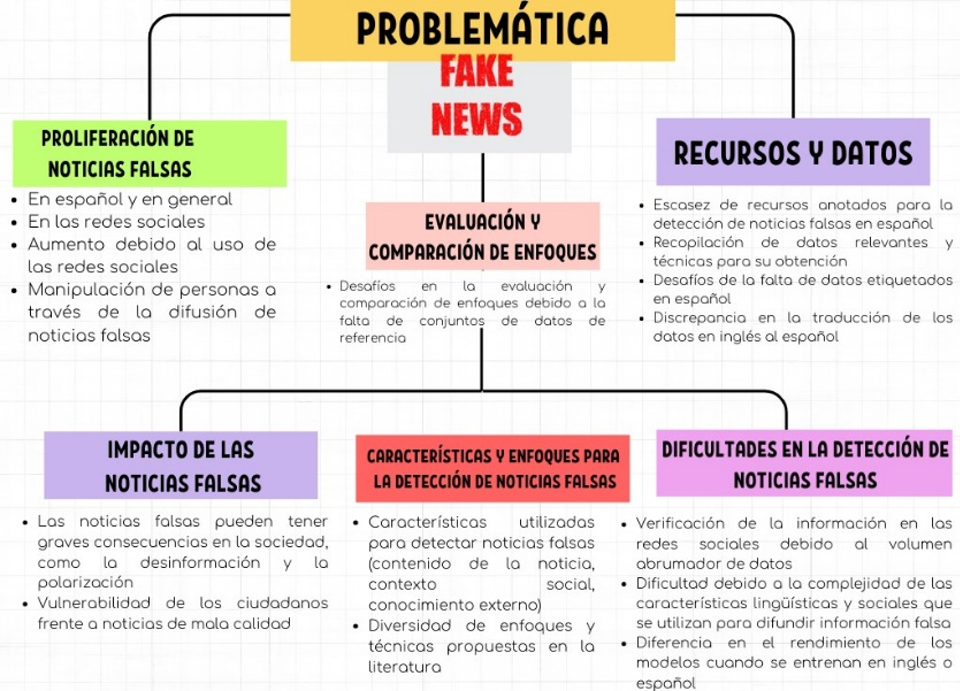
\includegraphics[width=\textwidth]{Imagenes/mapaConceptual1.png}
    \caption{Mapa Conceptual 1: Taxonomía del problema de desinformación y fraude digital en la era de la IA.}
    \label{fig:mapa_problema}
\end{figure}

\subsection{El Desafío Específico del Español}

El español, como la cuarta lengua más hablada del mundo con más de 500 millones de hablantes nativos \cite{acosta2019construccion}, presenta desafíos únicos para la detección automatizada de desinformación. A pesar de su importancia demográfica y económica, existe una notable escasez de recursos computacionales especializados para la detección de noticias falsas en español, en comparación con los abundantes recursos disponibles para el inglés \cite{posadas2019detection}.

Esta brecha de recursos se manifiesta en:
\begin{itemize}
    \item \textbf{Escasez de corpus etiquetados:} Limitados conjuntos de datos de entrenamiento en español para modelos de detección
    \item \textbf{Variabilidad dialectal:} La diversidad regional del español presenta desafíos adicionales para modelos generalizables
    \item \textbf{Contexto cultural específico:} Los patrones de desinformación varían según el contexto sociocultural hispanoamericano
    \item \textbf{Herramientas de detección limitadas:} Pocas soluciones tecnológicas disponibles para comunidades hispanohablantes
\end{itemize}

\subsection{La Complejidad Técnica del Problema}

La detección automatizada de \glspl{noticiafalsa} constituye un problema técnico multifacético que requiere la integración de múltiples disciplinas. Como documenta la literatura reciente \cite{singh2023comprehensive}, los desafíos incluyen:

\begin{itemize}
    \item \textbf{Análisis semántico profundo:} Necesidad de comprender el contexto y las implicaciones sutiles del contenido mediante técnicas de \gls{pln}
    \item \textbf{Detección de patrones estilométricos:} Identificación de características lingüísticas que indiquen autoría maliciosa \cite{tsai2023stylometric}
    \item \textbf{Procesamiento en tiempo real:} Capacidad de analizar el volumen masivo de contenido generado diariamente usando \gls{ml}
    \item \textbf{Adaptación a contenido sintético:} Detección de texto generado por modelos de \gls{ia} cada vez más sofisticados \cite{su2023adapting}
    \item \textbf{Robustez ante ataques adversariales:} Resistencia a intentos deliberados de evadir la detección
    \item \textbf{Optimización de \glspl{hiperparametro}:} Calibración de parámetros del modelo para maximizar el rendimiento
\end{itemize}

Dada la sofisticación de estas amenazas, se requieren soluciones tecnológicas igualmente avanzadas para combatir el fraude digital, como se esquematiza en la Figura \ref{fig:mapa_soluciones}. Este trabajo se centra en el desarrollo de tales soluciones, con un enfoque particular en el idioma español y la comparación sistemática de paradigmas tecnológicos complementarios.

\begin{figure}[h!]
    \centering
    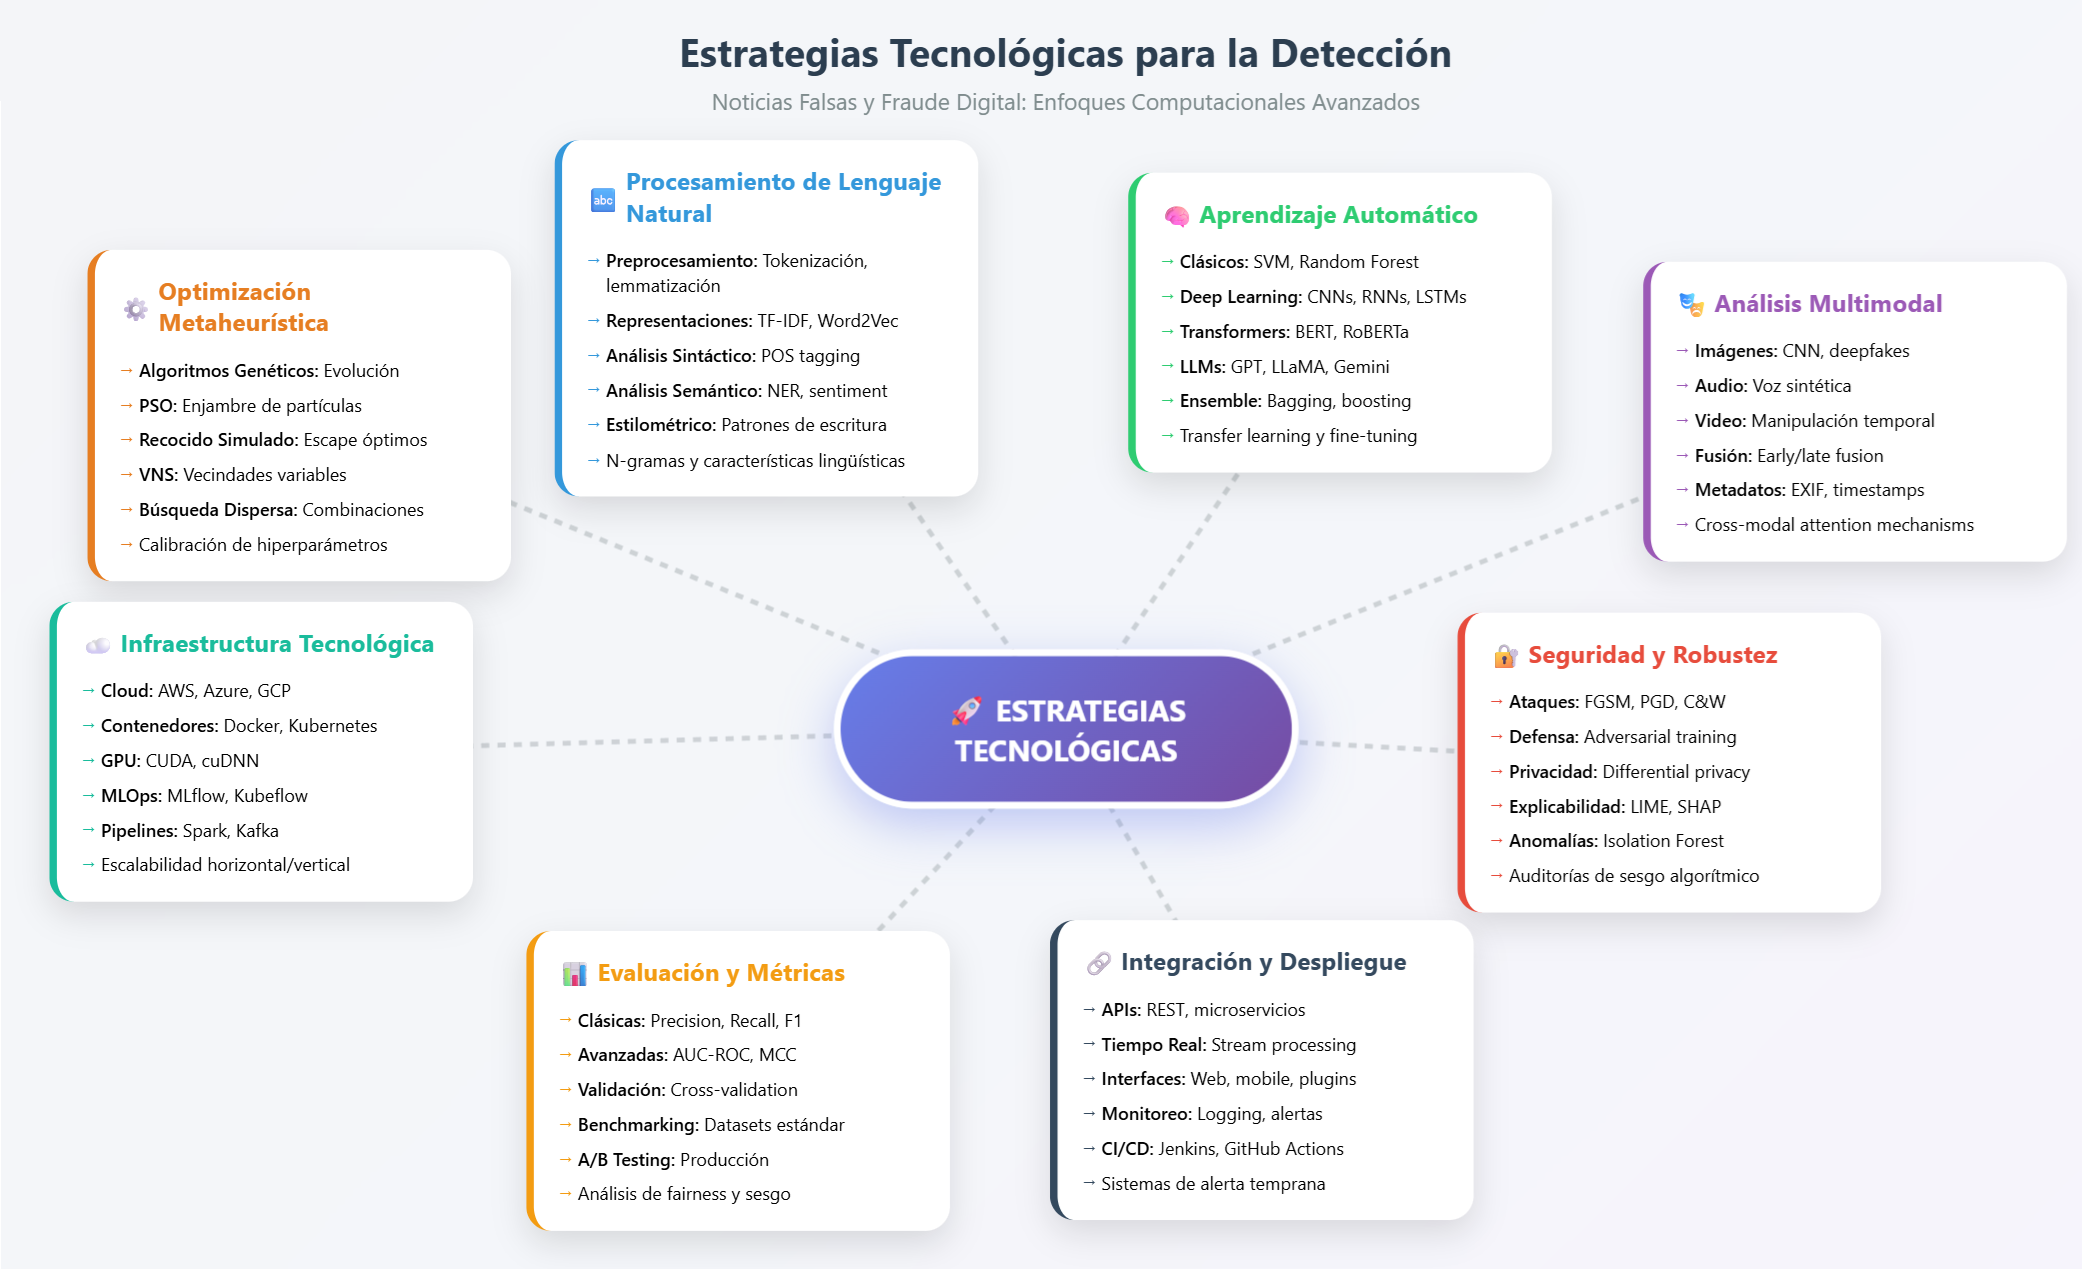
\includegraphics[width=\textwidth]{Imagenes/mapaConceptual2.png}
    \caption{Mapa Conceptual 2: Estrategias tecnológicas para la detección de fraude digital.}
    \label{fig:mapa_soluciones}
\end{figure}

\section{Motivación}

La motivación para llevar a cabo esta investigación se fundamenta en una combinación de experiencias personales observadas y la identificación de una brecha crítica en la protección tecnológica de las comunidades hispanohablantes.

\subsection{Impacto Personal y Social Observado}

Durante el desarrollo de esta investigación, se observaron múltiples casos en el entorno cercano donde personas fueron víctimas de fraude digital sofisticado. Estos casos incluyeron desde estafas de inversión disfrazadas de noticias financieras legítimas, hasta esquemas de phishing que aprovechaban eventos noticiosos actuales para parecer creíbles. Las víctimas, frecuentemente personas de edad avanzada o con menor exposición a tecnología digital, sufrieron no solo pérdidas económicas significativas, sino también impacto psicológico profundo, incluyendo sentimientos de vergüenza, ansiedad y pérdida de confianza en medios digitales.

\subsection{Vulnerabilidad de Poblaciones Específicas}

La investigación en psicología cognitiva aplicada a la desinformación \cite{ali2021fake} ha demostrado que ciertos grupos demográficos son particularmente vulnerables:

\begin{itemize}
    \item \textbf{Adultos mayores:} Mayor susceptibilidad a heurísticas de credibilidad basadas en autoridad percibida
    \item \textbf{Poblaciones con menor alfabetización digital:} Limitada capacidad para evaluar la legitimidad de fuentes online
    \item \textbf{Comunidades con acceso limitado a información:} Mayor dependencia de redes sociales como fuente primaria de noticias
    \item \textbf{Hablantes nativos de español:} Menor disponibilidad de herramientas de verificación en su idioma nativo
\end{itemize}

\subsection{Urgencia Tecnológica}

El rápido avance en modelos generativos de IA, como GPT-3 \cite{brown2020language} y sus sucesores, ha reducido significativamente las barreras técnicas para la creación de contenido falso convincente. Esta democratización de la capacidad de generar desinformación \cite{su2023fake} crea una urgencia imperativa para desarrollar defensas tecnológicas igualmente sofisticadas.

Impulsado por la necesidad de crear defensas tecnológicas más robustas y específicamente adaptadas para la comunidad hispanohablante, el presente trabajo se centra en desarrollar, comparar y validar métodos computacionales avanzados para la detección y prevención del fraude digital, con el objetivo final de contribuir a la protección de las poblaciones más vulnerables frente a estas amenazas emergentes.

\section{Justificación}

Esta investigación se justifica desde múltiples perspectivas: la brecha tecnológica existente, la novedad metodológica del enfoque, y la necesidad social de herramientas especializadas para el español.

\subsection{Brecha Tecnológica en Recursos para el Español}

El español, con más de 500 millones de hablantes nativos distribuidos en 21 países, representa un vasto ecosistema digital que ha sido históricamente subatendido en términos de herramientas especializadas para la detección de desinformación. Mientras que para el inglés existen múltiples datasets de gran escala como LIAR, FakeNewsNet, y CREDBANK \cite{hu2022deep}, los recursos equivalentes en español son limitados y fragmentados.

El estado del arte actual en español se basa principalmente en cuatro corpus principales:
\begin{itemize}
    \item \textbf{Corpus de Acosta (2019):} 598 noticias \cite{acosta2019construccion}
    \item \textbf{Spanish Fake News Corpus:} 971 noticias \cite{posadas2019detection}
    \item \textbf{Corpus de Tretiakov (2022):} 1,958 noticias \cite{tretiakov2022detection}
    \item \textbf{Spanish Political Fake News:} 57,000+ noticias \cite{blanco2024enhancing}
\end{itemize}

Esta fragmentación crea una barrera significativa para el desarrollo de modelos robustos y generalizables.

\subsection{Novedad Metodológica: Enfoque Evolutivo Comparativo}

La novedad principal de esta investigación radica en su enfoque evolutivo que compara sistemáticamente dos paradigmas fundamentalmente diferentes de la Inteligencia Artificial en el mismo contexto aplicado:

\subsubsection{Paradigma Clásico Optimizado}
\begin{itemize}
    \item \textbf{Representación textual:} Bolsa de Palabras (BoW) con ponderación TF-IDF
    \item \textbf{Optimización:} Algoritmos metaheurísticos para calibración de hiperparámetros
    \item \textbf{Clasificador:} Máquina de Vectores de Soporte (SVM) optimizada
    \item \textbf{Ventajas:} Eficiencia computacional, interpretabilidad, menor dependencia de hardware especializado
\end{itemize}

\subsubsection{Paradigma de Deep Learning}
\begin{itemize}
    \item \textbf{Representación textual:} Embeddings contextuales dinámicos
    \item \textbf{Modelo base:} DistilBERT pre-entrenado \cite{sanh2019distilbert}
    \item \textbf{Técnica:} Fine-tuning con optimización de hiperparámetros
    \item \textbf{Ventajas:} Comprensión semántica profunda, captura de relaciones contextuales complejas
\end{itemize}

\subsection{Contribución Científica Multidimensional}

Esta investigación ofrece contribuciones en múltiples dimensiones:

\subsubsection{Contribución a Recursos Lingüísticos}
\begin{itemize}
    \item \textbf{Corpus unificado:} Integración y estandarización de los principales corpus en español
    \item \textbf{Metodología de unificación:} Protocolo replicable para integrar datasets heterogéneos
    \item \textbf{Benchmarking:} Establecimiento de líneas base comparativas para futura investigación
\end{itemize}

\subsubsection{Contribución Metodológica}
\begin{itemize}
    \item \textbf{Optimización metaheurística:} Aplicación sistemática de algoritmos bio-inspirados para calibración de hiperparámetros en ambos paradigmas
    \item \textbf{Análisis comparativo riguroso:} Evaluación exhaustiva usando métricas múltiples y validación cruzada
    \item \textbf{Transferencia tecnológica:} Implementación práctica en aplicaciones web containerizadas
\end{itemize}

\subsubsection{Contribución Aplicada}
\begin{itemize}
    \item \textbf{Herramientas funcionales:} Aplicaciones web deployables para análisis en tiempo real
    \item \textbf{Código abierto:} Disponibilidad pública de implementaciones para reproducibilidad
    \item \textbf{Impacto social directo:} Herramientas utilizables por comunidades hispanohablantes
\end{itemize}

\subsection{Relevancia en el Contexto de LLMs}

Con el advenimiento de Grandes Modelos de Lenguaje como GPT-3 \cite{brown2020language}, LLaMA \cite{touvron2023llama}, y Gemini \cite{gemini2023family}, la generación de contenido sintético convincente se ha democratizado significativamente. Esta evolución hace que la investigación en detección sea más urgente y relevante, particularmente para idiomas como el español que han recibido menor atención en el desarrollo de contramedidas tecnológicas.

\section{Objetivos}

\subsection*{Objetivo General}
Desarrollar un método computacional basado en algoritmos metaheurísticos y modelos de lenguaje para detectar noticias falsas y fraude digital en español.

\subsection*{Objetivos Específicos}

\begin{itemize}
    \item Recopilar y procesar un conjunto de datos diverso a partir de múltiples corpus en español, y enriquecerlo mediante técnicas de \textit{web scraping} para entrenar y evaluar los sistemas de detección.
    
    \item Implementar un sistema de detección inicial que utilice técnicas de Procesamiento del Lenguaje Natural (Bolsa de Palabras) y algoritmos metaheurísticos.
    
    \item Desarrollar un sistema de detección avanzado mediante el ajuste fino (\textit{fine-tuning}) de un modelo de lenguaje profundo (\texttt{DistilBERT}), optimizando su rendimiento a través de la calibración de hiperparámetros.
    
    \item Realizar un análisis comparativo del rendimiento entre el enfoque metaheurístico y el modelo de lenguaje, utilizando un conjunto completo de métricas de evaluación (Exactitud, Precisión, Exhaustividad y F1-Score).
    
    \item Desarrollar un prototipo de aplicación web funcional, contenerizada con \texttt{Docker}, para demostrar la aplicabilidad práctica del modelo de mayor rendimiento en el análisis de URLs para categorizar contenido digital como fraudulento o legítimo.
\end{itemize}

\section{Alcance y Limitaciones}

\subsection{Alcance}

\subsubsection{Alcance Lingüístico y Cultural}
\begin{itemize}
    \item \textbf{Idioma objetivo:} El proyecto se centra exclusivamente en textos en español, abarcando múltiples variedades regionales representadas en los corpus utilizados
    \item \textbf{Dominio de aplicación:} Detección de noticias falsas como caso de uso principal, con extensibilidad demostrada hacia otros tipos de fraude digital
    \item \textbf{Contexto geográfico:} Cobertura de múltiples países hispanohablantes a través de los corpus integrados
\end{itemize}

\subsubsection{Alcance Técnico}
\begin{itemize}
    \item \textbf{Modalidad de datos:} Procesamiento exclusivo de contenido textual (no multimodal)
    \item \textbf{Tipo de clasificación:} Clasificación binaria supervisada (FALSO/REAL)
    \item \textbf{Arquitecturas evaluadas:} Comparación sistemática entre enfoques clásicos optimizados y modelos Transformer
    \item \textbf{Implementación práctica:} Desarrollo de aplicaciones web funcionales y containerizadas
\end{itemize}

\subsubsection{Alcance Metodológico}
\begin{itemize}
    \item \textbf{Optimización metaheurística:} Aplicación de tres algoritmos bio-inspirados para calibración de hiperparámetros
    \item \textbf{Validación experimental:} Uso de validación cruzada estratificada y métricas múltiples
    \item \textbf{Reproducibilidad:} Documentación completa y código fuente disponible
\end{itemize}

\subsection{Limitaciones}

\subsubsection{Limitaciones de Datos}
\begin{itemize}
    \item \textbf{Dependencia de corpus existentes:} El rendimiento está condicionado por la calidad y representatividad de los corpus disponibles en español
    \item \textbf{Sesgos inherentes:} Posibles sesgos temporales, temáticos o geográficos presentes en las fuentes originales
    \item \textbf{Evolución del lenguaje:} Los modelos pueden no capturar patrones emergentes en desinformación generada por IA más reciente
    \item \textbf{Etiquetado ground truth:} Dependencia de la calidad del etiquetado manual en los corpus originales
\end{itemize}

\subsubsection{Limitaciones Técnicas}
\begin{itemize}
    \item \textbf{Recursos computacionales:} El entrenamiento de modelos Transformer requiere hardware especializado (GPU) y tiempos de cómputo extensos (12-72+ horas)
    \item \textbf{Escalabilidad en tiempo real:} Los prototipos funcionan bajo demanda, no están optimizados para procesamiento de streams masivos
    \item \textbf{Generalización cross-domain:} Los modelos están específicamente entrenados para noticias, la efectividad en otros tipos de fraude digital es inferencial
    \item \textbf{Robustez adversarial:} No se evalúa específicamente la resistencia a ataques de evasión intencionales
\end{itemize}

\subsubsection{Limitaciones Operacionales}
\begin{itemize}
    \item \textbf{Herramienta de apoyo:} Los sistemas desarrollados son herramientas de apoyo a la decisión, no reemplazan el juicio humano experto
    \item \textbf{Verificación absoluta:} La determinación definitiva de veracidad puede requerir investigación periodística especializada
    \item \textbf{Contexto dinámico:} Los patrones de desinformación evolucionan constantemente, requiriendo actualización periódica de los modelos
    \item \textbf{Consideraciones éticas:} No se abordan explícitamente implicaciones de sesgo algorítmico o impacto en libertad de expresión
\end{itemize}

\subsubsection{Limitaciones de Evaluación}
\begin{itemize}
    \item \textbf{Métricas tradicionales:} La evaluación se basa en métricas estándar que pueden no capturar completamente la complejidad del problema
    \item \textbf{Validación temporal:} No se realiza validación temporal explícita con datos de períodos posteriores al entrenamiento
    \item \textbf{Análisis de errores:} El análisis cualitativo de errores es limitado debido al volumen de datos procesado
\end{itemize}

\section{Contribuciones Esperadas}

\subsection{Contribuciones Teóricas}
\begin{itemize}
    \item \textbf{Metodología comparativa:} Marco sistemático para comparar paradigmas clásicos y modernos en detección de desinformación
    \item \textbf{Optimización metaheurística:} Aplicación novedosa de algoritmos bio-inspirados para calibración de modelos Transformer
    \item \textbf{Análisis de trade-offs:} Caracterización cuantitativa de compromisos entre eficiencia computacional y rendimiento predictivo
\end{itemize}

\subsection{Contribuciones Prácticas}
\begin{itemize}
    \item \textbf{Corpus unificado:} Recurso consolidado para investigación futura en español
    \item \textbf{Herramientas funcionales:} Aplicaciones deployables para uso comunitario
    \item \textbf{Código abierto:} Implementaciones reproducibles y extensibles
\end{itemize}

\subsection{Contribuciones Sociales}
\begin{itemize}
    \item \textbf{Protección comunitaria:} Herramientas accesibles para comunidades hispanohablantes
    \item \textbf{Democratización tecnológica:} Reducción de la brecha digital en herramientas de verificación
    \item \textbf{Capacitación y concientización:} Contribución a la alfabetización digital en detección de desinformación
\end{itemize}

\section{Organización del Documento}

Este documento se estructura de manera lógica y progresiva para guiar al lector a través del proceso completo de investigación, desarrollo y evaluación:

\begin{itemize}
    \item \textbf{Capítulo 2 - Marco Teórico:} Establece los fundamentos teóricos que sustentan ambas metodologías, desde técnicas clásicas de representación textual hasta arquitecturas Transformer modernas, incluyendo principios de optimización metaheurística.

    \item \textbf{Capítulo 3 - Estado del Arte:} Presenta una revisión comprehensiva y organizada temáticamente de la literatura relevante, identificando brechas de conocimiento y posicionando esta investigación en el contexto científico actual.

    \item \textbf{Capítulo 4 - Metodología:} Detalla la metodología evolutiva seguida, desde la construcción del corpus unificado hasta la implementación y optimización de ambos paradigmas de detección.

    \item \textbf{Capítulo 5 - Análisis de Resultados:} Presenta y compara exhaustivamente los resultados obtenidos por ambas metodologías, incluyendo análisis estadístico, métricas de rendimiento y discusión de fortalezas y limitaciones.

    \item \textbf{Capítulo 6 - Implementación de Prototipo:} Describe la arquitectura, desarrollo y despliegue de las aplicaciones web funcionales que demuestran la viabilidad práctica de los modelos desarrollados.

    \item \textbf{Capítulo 7 - Conclusiones y Trabajo Futuro:} Sintetiza los hallazgos principales, evalúa el cumplimiento de objetivos, y propone direcciones específicas para investigación futura en el campo.
\end{itemize}

Cada capítulo se construye sobre los anteriores, manteniendo coherencia narrativa y técnica a lo largo del documento, mientras proporciona la profundidad analítica necesaria para validar las contribuciones científicas y prácticas de esta investigación.
%!TEX root = ../ICR.tex
\chapter{Marco Teórico \label{cap:MarcoTeorico}}

En esta sección se describen las bases teóricas y los conceptos fundamentales que sustentan las dos metodologías de detección de noticias falsas desarrolladas en este proyecto de investigación. Aunque las técnicas son aplicables a diferentes tipos de fraude digital, el enfoque específico se centra en la detección de desinformación periodística. Se abordan desde las técnicas clásicas de representación de texto y optimización metaheurística, hasta los paradigmas de aprendizaje profundo que definen el estado del arte actual.

\section{Detección de Noticias Falsas: Fundamentos y Extensibilidad}
\label{sec:deteccion_noticias_falsas}

La detección de noticias falsas constituye un problema multifacético que requiere un enfoque interdisciplinario, con metodologías que pueden extenderse a otros tipos de fraude digital. La desinformación se caracteriza por ser información deliberadamente falsa o engañosa que se presenta como noticia legítima \cite{bondielli2019survey}. Esta problemática ha evolucionado significativamente con el advenimiento de las redes sociales y los medios digitales, donde la velocidad de propagación supera ampliamente la capacidad de verificación tradicional.

En el contexto de la detección automatizada, se han explorado diferentes enfoques y técnicas. Das et al. \cite{das2022heuristic} propusieron un marco de ensamblaje basado en incertidumbre e impulsado por heurísticas para la detección de noticias falsas en tuits y artículos de noticias. Este enfoque parte de la premisa de que diferentes modelos pueden tener distintas fortalezas y debilidades, y que la combinación inteligente de múltiples predictores puede superar las limitaciones individuales.

El equipo de la Southern Methodist University presentó una solución pionera utilizando procesamiento de lenguaje natural y aprendizaje profundo para analizar tanto titulares como el contenido completo de las noticias \cite{thota2018fake}. Su trabajo estableció un precedente importante al demostrar la viabilidad de la vectorización TF-IDF combinada con redes neuronales densas.

Complementariamente, se ha propuesto un enfoque basado en análisis estilométrico utilizando Procesamiento del Lenguaje Natural (PLN) y Reconocimiento de Entidades Nombradas (NER) para identificar patrones lingüísticos que sugieran baja veracidad de la información \cite{tsai2023stylometric}. Este enfoque aprovecha la hipótesis de que los autores de contenido falso pueden exhibir patrones de escritura distintivos.

\subsection{Impacto Social y Desafíos de la Desinformación}

La rápida propagación de las noticias falsas a través de las redes sociales puede tener graves consecuencias en la sociedad. Como documentan Ali y Zain-Ul-Abdin \cite{ali2020posttruth}, la desinformación puede:

\begin{itemize}
    \item \textbf{Distorsionar la realidad:} Alterando la percepción pública de eventos y hechos
    \item \textbf{Manipular la opinión pública:} Influenciando procesos democráticos y decisiones sociales
    \item \textbf{Incitar a la violencia:} Promoviendo comportamientos agresivos basados en información errónea
    \item \textbf{Difundir propaganda política:} Siendo utilizada como herramienta de influencia partidista
    \item \textbf{Fomentar el odio:} Exacerbando divisiones sociales y promoviendo discriminación
    \item \textbf{Provocar pánico:} Especialmente en contextos de crisis sanitarias como la pandemia de COVID-19 \cite{perez2020fake}
\end{itemize}

\subsection{El Problema de las Heurísticas Cognitivas}

La investigación de Ali et al. \cite{ali2021fake} ha demostrado que las heurísticas cognitivas humanas, como la popularidad social (número de "me gusta" o compartidos), influyen significativamente en la percepción de credibilidad. Este fenómeno complica la detección, ya que el contenido falso puede volverse viral precisamente por aprovechar estos sesgos cognitivos.

\subsection{Diferenciación Técnica y Transferibilidad: Noticias Falsas vs. Fraude Digital}

Es crucial establecer una distinción técnica clara entre los dominios de aplicación, ya que aunque comparten características computacionales, representan problemas con diferentes objetivos, audiencias y patrones:

\subsubsection{Características Distintivas por Dominio}

\begin{table}[htbp]
\centering
\adjustbox{width=\textwidth,center}{%
\small
\begin{tabular}{|l|l|l|}
\hline
\rowcolor{UAMPurple!20}
\textbf{Aspecto} & \textbf{Noticias Falsas} & \textbf{Fraude Digital} \\
\hline
\textbf{Objetivo primario} & 
\begin{tabular}[t]{@{}l@{}}Manipulación de opinión pública,\\influencia política/social\end{tabular} & 
\begin{tabular}[t]{@{}l@{}}Beneficio económico ilícito,\\acceso no autorizado a recursos\end{tabular} \\
\hline
\textbf{Formato típico} & 
\begin{tabular}[t]{@{}l@{}}Artículos periodísticos,\\imitando medios legítimos\end{tabular} & 
\begin{tabular}[t]{@{}l@{}}Emails de phishing, anuncios\\de inversión, ofertas comerciales\end{tabular} \\
\hline
\textbf{Audiencia objetivo} & 
\begin{tabular}[t]{@{}l@{}}Consumidores de noticias, votantes,\\opinión pública general\end{tabular} & 
\begin{tabular}[t]{@{}l@{}}Potenciales víctimas económicas,\\usuarios con activos digitales\end{tabular} \\
\hline
\textbf{Métrica de éxito} & 
\begin{tabular}[t]{@{}l@{}}Viralidad, alcance,\\influencia en opinión\end{tabular} & 
\begin{tabular}[t]{@{}l@{}}Cantidad de dinero/\\información obtenida\end{tabular} \\
\hline
\textbf{Indicadores lingüísticos} & 
\begin{tabular}[t]{@{}l@{}}Imitación de estilo periodístico,\\fuentes falsas, sensacionalismo político\end{tabular} & 
\begin{tabular}[t]{@{}l@{}}Urgencia económica, ofertas "limitadas",\\solicitudes de información personal\end{tabular} \\
\hline
\textbf{Temporalidad} & 
\begin{tabular}[t]{@{}l@{}}Eventos actuales,\\ciclos noticiosos\end{tabular} & 
\begin{tabular}[t]{@{}l@{}}Atemporales, aprovechan\\tendencias económicas\end{tabular} \\
\hline
\end{tabular}
}
\caption{Diferencias técnicas entre dominios de desinformación}
\label{tab:diferencias_dominios}
\end{table}

\subsubsection{Fundamentos de la Transferibilidad Metodológica}

A pesar de sus diferencias conceptuales, ambos dominios comparten características computacionales fundamentales que justifican la transferibilidad de la metodología desarrollada:

\begin{itemize}
    \item \textbf{Naturaleza textual primaria}: Ambos dominios se basan en contenido textual como vector principal de engaño
    \item \textbf{Problema de clasificación binaria}: Se reducen a problemas de clasificación legítimo/malicioso
    \item \textbf{Características estilométricas}: Ambos pueden exhibir patrones lingüísticos distintivos detectables
    \item \textbf{Optimización de hiperparámetros}: Ambos se benefician de técnicas de calibración metaheurística
    \item \textbf{Evaluación mediante métricas estándar}: Utilizan las mismas métricas de clasificación (precisión, recall, F1-Score)
\end{itemize}

\subsubsection{Protocolo de Transferencia Metodológica}

Para aplicar la metodología desarrollada a detección de fraude digital, se requiere el siguiente protocolo de adaptación:

\begin{enumerate}
    \item \textbf{Construcción de corpus específico}: Recopilar y etiquetar datos representativos del tipo de fraude digital objetivo
    \item \textbf{Ajuste de preprocesamiento}: Adaptar técnicas de limpieza según las características del nuevo dominio (emails vs. artículos)
    \item \textbf{Re-calibración de hiperparámetros}: Aplicar los mismos algoritmos metaheurísticos pero re-optimizar para el nuevo corpus
    \item \textbf{Incorporación de características específicas}: Añadir features relevantes al nuevo dominio (URLs sospechosas, patrones de solicitud de información)
    \item \textbf{Validación cross-domain}: Evaluar la transferencia utilizando métricas de generalización
\end{enumerate}

\textbf{Enfoque de esta investigación}: Este proyecto desarrolla y valida la metodología en el dominio de noticias falsas en español, estableciendo las bases técnicas para su posterior transferencia a otros tipos de fraude digital. La elección de noticias falsas como dominio inicial se justifica por: (1) disponibilidad de corpus etiquetados, (2) relevancia social en comunidades hispanohablantes, y (3) menor complejidad técnica que permite validar la metodología base antes de extensiones más complejas.

\section{Representación de Texto: Desde BoW hasta Embeddings Contextuales}
\label{sec:representacion_texto}

La evolución de las técnicas de representación textual ha sido fundamental para el progreso en PLN. Esta sección aborda desde los métodos clásicos hasta las representaciones más sofisticadas utilizadas en esta tesis.

\subsection{Bolsa de Palabras (Bag-of-Words - BoW)}

El modelo de Bolsa de Palabras (BoW) constituye una de las técnicas más fundamentales para la representación de texto. A pesar de su simplicidad, sigue siendo relevante como línea base y componente en sistemas híbridos. El proceso implica:

\begin{enumerate}
    \item \textbf{Construcción del vocabulario:} Creación de un diccionario con todas las palabras únicas presentes en el corpus de documentos
    \item \textbf{Vectorización:} Representación de cada documento como un vector disperso, donde cada dimensión corresponde a una palabra del vocabulario y su valor representa la frecuencia de aparición
\end{enumerate}

Aunque este método ignora la gramática y el orden de las palabras, ha demostrado ser efectivo como base para métodos más sofisticados y fue fundamental en los primeros trabajos de clasificación de noticias en español \cite{acosta2019construccion}.

\subsection{Ponderación TF-IDF (Term Frequency-Inverse Document Frequency)}

La técnica TF-IDF mejora significativamente la representación BoW al introducir ponderación semántica. Se calcula como el producto de dos componentes:

\begin{equation}
\text{TF-IDF}(t,d,D) = \text{TF}(t,d) \times \text{IDF}(t,D)
\end{equation}

Donde:
\begin{itemize}
    \item \textbf{Frecuencia de Término (TF):} $\text{TF}(t,d) = \frac{f_{t,d}}{\sum_{t' \in d} f_{t',d}}$ - frecuencia relativa del término $t$ en el documento $d$
    \item \textbf{Frecuencia Inversa de Documento (IDF):} $\text{IDF}(t,D) = \log\frac{|D|}{|\{d \in D : t \in d\}|}$ - importancia global del término en la colección
\end{itemize}

Esta ponderación asigna mayor peso a términos que son frecuentes en un documento específico pero raros en el corpus general, mejorando la capacidad discriminativa del modelo \cite{thota2018fake}.

\subsection{Limitaciones de los Métodos Clásicos}

Los enfoques basados en BoW y TF-IDF presentan limitaciones fundamentales:
\begin{itemize}
    \item \textbf{Pérdida de información secuencial:} No capturan el orden ni la estructura sintáctica
    \item \textbf{Problema de dispersidad:} Generan representaciones muy dispersas en vocabularios grandes
    \item \textbf{Ausencia de semántica:} No modelan relaciones semánticas entre palabras
    \item \textbf{Falta de contexto:} Una palabra tiene la misma representación independientemente del contexto
\end{itemize}

\section{La Revolución Transformer y los Modelos de Lenguaje Modernos}
\label{sec:transformers_modelos_lenguaje}

\subsection{La Arquitectura Transformer: Fundamentos}

La arquitectura Transformer, introducida por Vaswani et al. \cite{vaswani2017attention} en el trabajo seminal "Attention Is All You Need", revolucionó el campo del PLN. Su innovación principal radica en el mecanismo de \textbf{auto-atención (self-attention)}, que permite al modelo calcular representaciones ponderando dinámicamente la importancia de cada elemento en una secuencia con respecto a todos los demás elementos.

\subsubsection{Mecanismo de Atención Multi-Cabeza}

El mecanismo de atención se define matemáticamente como:

\begin{equation}
\text{Attention}(Q,K,V) = \text{softmax}\left(\frac{QK^T}{\sqrt{d_k}}\right)V
\end{equation}

Donde $Q$, $K$, y $V$ representan las matrices de consultas (queries), claves (keys) y valores (values), respectivamente. La atención multi-cabeza extiende este concepto:

\begin{equation}
\text{MultiHead}(Q,K,V) = \text{Concat}(\text{head}_1, ..., \text{head}_h)W^O
\end{equation}

Esta arquitectura permite capturar diferentes tipos de relaciones lingüísticas simultáneamente, superando las limitaciones de los modelos secuenciales previos como RNNs y LSTMs.

\subsection{BERT y la Era del Pre-entrenamiento Bidireccional}

BERT (Bidirectional Encoder Representations from Transformers) \cite{devlin2018bert} introdujo el paradigma de pre-entrenamiento bidireccional, entrenando el modelo para predecir palabras enmascaradas considerando tanto el contexto izquierdo como el derecho. Este enfoque genera representaciones contextuales más ricas que los modelos unidireccionales previos.

\subsubsection{Variantes de BERT para Eficiencia}

El éxito de BERT motivó el desarrollo de variantes más eficientes:
\begin{itemize}
    \item \textbf{DistilBERT} \cite{sanh2019distilbert}: Utiliza destilación de conocimiento para reducir el tamaño del modelo en un 40\% manteniendo el 97\% del rendimiento
    \item \textbf{TinyBERT} \cite{jiao2019tinybert}: Aplica destilación a nivel de transformador y predicción para crear modelos aún más compactos
\end{itemize}

\subsection{Aplicaciones en Detección de Noticias Falsas en Español}

Para el español específicamente, se han desarrollado modelos especializados y evaluaciones:
\begin{itemize}
    \item Martínez-Gallego et al. \cite{martinez2021fake} exploraron la aplicación de BERT y BETO (BERT en español), estableciendo líneas base importantes
    \item Blanco-Fernández et al. \cite{blanco2024enhancing} compararon sistemáticamente BERT y RoBERTa para detección de desinformación política
    \item Shushkevich et al. \cite{shushkevich2023improving} investigaron la mejora de clasificación multiclase usando datos aumentados con ChatGPT
\end{itemize}

\subsection{Grandes Modelos de Lenguaje (LLMs) y Nuevos Paradigmas}

\subsubsection{GPT-3 y el Paradigma Few-Shot}

GPT-3 \cite{brown2020language} marcó un hito al demostrar capacidades emergentes de few-shot learning. Con 175 mil millones de parámetros, mostró que los modelos de gran escala pueden realizar tareas sin ajuste fino específico, solo con ejemplos en el prompt.

\subsubsection{LLaMA y la Democratización de LLMs}

LLaMA \cite{touvron2023llama} representa el esfuerzo por democratizar el acceso a modelos de gran escala, proporcionando alternativas open-source a modelos propietarios. Su arquitectura optimizada permite un rendimiento competitivo con menor costo computacional.

\subsubsection{Modelos Multimodales: Gemini}

Gemini \cite{gemini2023family} introduce capacidades multimodales nativas, procesando texto, imágenes y audio de forma integrada. Esta capacidad es relevante para la detección de desinformación que cada vez más incorpora elementos multimedia.

\subsubsection{IA Constitucional}

El trabajo de Bai et al. \cite{bai2022constitutional} sobre IA Constitucional aborda la alineación y seguridad de los LLMs, estableciendo principios para entrenar modelos más seguros y alineados con valores humanos. Este enfoque es crucial cuando los LLMs se utilizan para tareas de detección de desinformación.

\subsection{El Doble Rol de los LLMs en Detección}

La investigación reciente ha revelado que los LLMs presentan un doble rol:
\begin{itemize}
    \item \textbf{Como "Buenos Consejeros":} Pueden ser fine-tuned para detectar noticias falsas con alta precisión \cite{hu2024bad}
    \item \textbf{Como "Malos Actores":} Pueden generar desinformación convincente, complicando la detección \cite{su2023fake}
    \item \textbf{Adaptación Necesaria:} Los sistemas de detección deben adaptarse a la era de LLMs \cite{su2023adapting}
\end{itemize}

\section{Optimización Metaheurística en Detección de Fraude}
\label{sec:optimizacion_metaheuristica}

\subsection{Fundamentos de las Metaheurísticas}

Las metaheurísticas son estrategias de optimización de alto nivel que guían procesos de búsqueda para encontrar soluciones de alta calidad en espacios de búsqueda complejos. A diferencia de los algoritmos exactos, las metaheurísticas buscan soluciones "suficientemente buenas" en tiempo computacional razonable \cite{anselmo2013diseno}.

\subsubsection{Justificación del Uso de Metaheurísticas en Detección de Noticias Falsas}

La aplicación de metaheurísticas en este dominio se justifica por las siguientes características del problema:

\begin{itemize}
    \item \textbf{Espacio de hiperparámetros complejo:} Los modelos de clasificación (SVM, redes neuronales) tienen múltiples hiperparámetros interdependientes
    \item \textbf{Función objetivo no convexa:} Las métricas de rendimiento (F1-Score, precisión) no son funciones continuas y diferenciables
    \item \textbf{Interacciones no lineales:} Los hiperparámetros interactúan de manera compleja, haciendo ineficaces los métodos de optimización tradicionales
    \item \textbf{Múltiples óptimos locales:} El espacio de búsqueda presenta numerosos máximos locales que pueden atrapar algoritmos determinísticos
    \item \textbf{Eficiencia computacional:} Las metaheurísticas exploran el espacio de forma más inteligente que métodos exhaustivos como grid search
\end{itemize}

\subsubsection{Arquitectura General del Sistema Metaheurístico}

El framework metaheurístico desarrollado sigue una arquitectura modular que permite la intercambiabilidad de algoritmos:

\begin{equation}
\text{Sistema} = \{D, P, A, F, E\}
\end{equation}

Donde:
\begin{itemize}
    \item \textbf{D}: Dataset de noticias preprocesado
    \item \textbf{P}: Pipeline de preprocesamiento (tokenización, TF-IDF)
    \item \textbf{A}: Algoritmo metaheurístico (GA, PSO, SA, VNS, SS)
    \item \textbf{F}: Función objetivo (F1-Score en validación cruzada)
    \item \textbf{E}: Evaluador final en conjunto de prueba
\end{itemize}

\subsubsection{Entradas del Sistema Metaheurístico}

\textbf{1. Datos de Entrada:}
\begin{itemize}
    \item \textbf{Corpus textual:} Noticias en español con etiquetas binarias (REAL/FALSO)
    \item \textbf{División de datos:} 70\% entrenamiento, 10\% validación, 20\% prueba (estratificada)
    \item \textbf{Representación BoW:} Matriz dispersa TF-IDF de dimensión $n \times v$ donde $n$ es el número de documentos y $v$ el tamaño del vocabulario
\end{itemize}

\textbf{2. Espacio de Hiperparámetros:}

Para SVM con kernel RBF:
\begin{align}
C &\in [10^{-3}, 10^{3}] \text{ (parámetro de regularización)} \\
\gamma &\in [10^{-4}, 10^{1}] \text{ (parámetro del kernel RBF)} \\
\text{class\_weight} &\in \{\text{None}, \text{balanced}\} \text{ (balanceado de clases)}
\end{align}

Para TF-IDF:
\begin{align}
\text{max\_features} &\in [1000, 50000] \text{ (tamaño del vocabulario)} \\
\text{min\_df} &\in [1, 10] \text{ (frecuencia mínima de documento)} \\
\text{max\_df} &\in [0.7, 1.0] \text{ (frecuencia máxima de documento)} \\
\text{ngram\_range} &\in \{(1,1), (1,2), (1,3)\} \text{ (rango de n-gramas)}
\end{align}

\subsubsection{Preprocesamiento y Pipeline}

\textbf{Etapa 1: Limpieza Textual}
\begin{enumerate}
    \item \textbf{Normalización de caracteres:} Conversión a minúsculas, eliminación de acentos
    \item \textbf{Filtrado de contenido:} Eliminación de URLs, menciones (@), hashtags
    \item \textbf{Tokenización:} División en tokens usando expresiones regulares
    \item \textbf{Eliminación de stopwords:} Filtrado de palabras vacías en español
    \item \textbf{Validación de longitud:} Exclusión de textos demasiado cortos ($<$ 10 tokens)
\end{enumerate}

\textbf{Etapa 2: Vectorización TF-IDF}
\begin{equation}
\text{TF-IDF}(t,d) = \text{TF}(t,d) \times \log\left(\frac{N}{|\{d' : t \in d'\}|}\right)
\end{equation}

Donde $t$ es un término, $d$ un documento, $N$ el total de documentos, y el denominador cuenta documentos que contienen $t$.

\textbf{Etapa 3: Normalización}
Aplicación de normalización L2 para estabilizar el entrenamiento:
\begin{equation}
\mathbf{x}_{\text{norm}} = \frac{\mathbf{x}}{||\mathbf{x}||_2}
\end{equation}

\subsubsection{Algoritmos Metaheurísticos Implementados}

\textbf{1. Algoritmo Genético (GA)}

\textit{Inspiración biológica:} Evolución natural y selección de especies

\textit{Representación:} Cada individuo es un vector de hiperparámetros codificados
\begin{equation}
\text{Individuo} = [C, \gamma, \text{max\_features}, \text{min\_df}, \text{max\_df}, \text{ngram}]
\end{equation}

\textit{Operadores genéticos:}
\begin{itemize}
    \item \textbf{Selección:} Torneo de tamaño 3
    \item \textbf{Cruce:} Cruce uniforme con probabilidad 0.8
    \item \textbf{Mutación:} Mutación gaussiana con probabilidad 0.1
    \item \textbf{Elitismo:} Preservación del 10\% mejores individuos
\end{itemize}

\textit{Parámetros:}
\begin{align}
\text{Tamaño población} &= 30 \\
\text{Generaciones} &= 50 \\
\text{Tasa cruce} &= 0.8 \\
\text{Tasa mutación} &= 0.1
\end{align}

\textbf{2. Optimización por Enjambre de Partículas (PSO)}

\textit{Inspiración biológica:} Comportamiento de bandadas de aves y cardúmenes

\textit{Ecuaciones de movimiento:}
\begin{align}
v_{i}^{t+1} &= w \cdot v_{i}^{t} + c_1 \cdot r_1 \cdot (p_{i} - x_{i}^{t}) + c_2 \cdot r_2 \cdot (g - x_{i}^{t}) \\
x_{i}^{t+1} &= x_{i}^{t} + v_{i}^{t+1}
\end{align}

Donde:
\begin{itemize}
    \item $v_i^t$: velocidad de la partícula $i$ en iteración $t$
    \item $x_i^t$: posición de la partícula $i$ en iteración $t$
    \item $p_i$: mejor posición personal de la partícula $i$
    \item $g$: mejor posición global del enjambre
    \item $w$: factor de inercia ($w = 0.9$)
    \item $c_1, c_2$: factores de aceleración ($c_1 = c_2 = 2.0$)
    \item $r_1, r_2$: números aleatorios $\in [0,1]$
\end{itemize}

\textit{Parámetros:}
\begin{align}
\text{Tamaño enjambre} &= 30 \\
\text{Iteraciones} &= 50 \\
\text{Factor inercia} &= 0.9 \\
\text{Factores aceleración} &= 2.0
\end{align}

\textbf{3. Recocido Simulado Multi-arranque (MSA)}

\textit{Inspiración física:} Proceso de enfriamiento controlado en metalurgia

\textit{Criterio de aceptación:}
\begin{equation}
P(\text{aceptar}) = \begin{cases}
1 & \text{si } \Delta f \geq 0 \\
e^{\frac{\Delta f}{T}} & \text{si } \Delta f < 0
\end{cases}
\end{equation}

Donde $\Delta f = f(\text{nueva}) - f(\text{actual})$ y $T$ es la temperatura.

\textit{Esquema de enfriamiento:}
\begin{equation}
T_{k+1} = \alpha \cdot T_k, \quad \alpha = 0.95
\end{equation}

\textit{Parámetros:}
\begin{align}
\text{Temperatura inicial} &= 100.0 \\
\text{Temperatura final} &= 0.01 \\
\text{Factor enfriamiento} &= 0.95 \\
\text{Iteraciones por temperatura} &= 10 \\
\text{Número de arranques} &= 5
\end{align}

\textbf{4. Búsqueda en Vecindades Variables (VNS)}

\textit{Principio:} Cambio sistemático de estructuras de vecindad para escapar de óptimos locales

\textit{Estructuras de vecindad:}
\begin{itemize}
    \item $N_1$: Perturbación de un hiperparámetro aleatorio
    \item $N_2$: Perturbación de dos hiperparámetros aleatorios
    \item $N_3$: Perturbación de todos los hiperparámetros
\end{itemize}

\textit{Algoritmo general:}
\begin{enumerate}
    \item Inicializar solución $x$
    \item Para cada vecindad $k = 1, 2, 3$:
    \item \quad Generar $x'$ en $N_k(x)$
    \item \quad Aplicar búsqueda local desde $x'$ → $x''$
    \item \quad Si $f(x'') > f(x)$: $x = x''$, $k = 1$
    \item \quad Sino: $k = k + 1$
    \item Repetir hasta criterio de parada
\end{enumerate}

\textbf{5. Búsqueda Dispersa (SS)}

\textit{Principio:} Combinar soluciones de calidad y diversas para generar nuevas soluciones

\textit{Componentes principales:}
\begin{itemize}
    \item \textbf{Conjunto de referencia:} 10 soluciones (5 de calidad + 5 diversas)
    \item \textbf{Generación de subconjuntos:} Todas las combinaciones de tamaño 2
    \item \textbf{Método de combinación:} Promedio ponderado por fitness
    \item \textbf{Mejora:} Búsqueda local en nuevas soluciones
    \item \textbf{Actualización:} Reemplazo de peores soluciones
\end{itemize}

\subsubsection{Función Objetivo y Evaluación}

\textbf{Función objetivo principal:}
\begin{equation}
f(\theta) = \text{F1-Score}_{CV}(\theta)
\end{equation}

Donde $\theta$ representa el vector de hiperparámetros y $\text{F1-Score}_{CV}$ es el F1-Score promedio en validación cruzada estratificada de 5 pliegues.

\textbf{Métricas de evaluación secundarias:}
\begin{align}
\text{Precisión} &= \frac{TP}{TP + FP} \\
\text{Recall} &= \frac{TP}{TP + FN} \\
\text{F1-Score} &= \frac{2 \times \text{Precisión} \times \text{Recall}}{\text{Precisión} + \text{Recall}} \\
\text{Exactitud} &= \frac{TP + TN}{TP + TN + FP + FN}
\end{align}

\subsubsection{Etapas del Proceso Metaheurístico}

\textbf{Etapa 1: Inicialización}
\begin{enumerate}
    \item Cargar y dividir el dataset
    \item Definir espacios de búsqueda para hiperparámetros
    \item Inicializar población/enjambre según el algoritmo
    \item Configurar parámetros del algoritmo metaheurístico
\end{enumerate}

\textbf{Etapa 2: Evaluación de Fitness}
\begin{enumerate}
    \item Para cada configuración de hiperparámetros:
    \item \quad Construir pipeline TF-IDF + SVM
    \item \quad Entrenar en conjunto de entrenamiento
    \item \quad Evaluar en validación cruzada 5-fold
    \item \quad Calcular F1-Score promedio como fitness
\end{enumerate}

\textbf{Etapa 3: Evolución/Optimización}
\begin{enumerate}
    \item Aplicar operadores específicos del algoritmo
    \item Generar nuevas configuraciones candidatas
    \item Evaluar fitness de nuevas configuraciones
    \item Actualizar población/enjambre según criterios del algoritmo
    \item Verificar criterios de convergencia
\end{enumerate}

\textbf{Etapa 4: Selección Final}
\begin{enumerate}
    \item Identificar la mejor configuración encontrada
    \item Re-entrenar modelo con configuración óptima
    \item Evaluar en conjunto de prueba independiente
    \item Reportar métricas finales
\end{enumerate}

\subsubsection{Salidas del Sistema Metaheurístico}

\textbf{1. Configuración Óptima de Hiperparámetros:}
\begin{itemize}
    \item Valores óptimos para cada hiperparámetro del modelo
    \item Historia de convergencia del algoritmo
    \item Número de evaluaciones realizadas
    \item Tiempo total de optimización
\end{itemize}

\textbf{2. Modelo Entrenado Optimizado:}
\begin{itemize}
    \item Vectorizador TF-IDF configurado
    \item Clasificador SVM entrenado
    \item Pipeline completo listo para predicción
\end{itemize}

\textbf{3. Métricas de Rendimiento:}
\begin{itemize}
    \item F1-Score, Precisión, Recall, Exactitud en conjunto de prueba
    \item Matriz de confusión
    \item Curvas de convergencia
    \item Análisis de importancia de hiperparámetros
\end{itemize}

\textbf{4. Análisis Comparativo:}
\begin{itemize}
    \item Comparación entre algoritmos metaheurísticos
    \item Análisis de eficiencia computacional
    \item Estudio de robustez y estabilidad
\end{itemize}

En el contexto de la detección de noticias falsas, las metaheurísticas abordan varios problemas de optimización, con metodologías transferibles a otros tipos de fraude digital:
\begin{itemize}
    \item \textbf{Calibración de hiperparámetros:} Optimización de parámetros de modelos de ML/DL
    \item \textbf{Selección de características:} Identificación de subconjuntos óptimos de variables
    \item \textbf{Arquitectura neural:} Diseño automático de topologías de red
    \item \textbf{Balanceado de datos:} Optimización de técnicas de muestreo
\end{itemize}

\subsubsection{Comparación de Algoritmos Metaheurísticos}

La Tabla \ref{tab:comparacion_metaheuristicas} presenta una comparación sistemática de los cinco algoritmos implementados, destacando sus características distintivas, ventajas y limitaciones en el contexto de optimización de hiperparámetros para detección de noticias falsas.

\begin{table}[htbp]
\centering
\adjustbox{width=\textwidth,center}{%
\small
\begin{tabular}{|l|l|l|l|l|}
\hline
\rowcolor{UAMPurple!20}
\textbf{Algoritmo} & \textbf{Inspiración} & \textbf{Fortalezas} & \textbf{Limitaciones} & \textbf{Parámetros Clave} \\
\hline
\textbf{GA} & Evolución biológica & 
\begin{tabular}[t]{@{}l@{}}Exploración global robusta\\Paralelización natural\\Buena diversidad poblacional\end{tabular} & 
\begin{tabular}[t]{@{}l@{}}Convergencia lenta\\Muchos parámetros a ajustar\\Puede estancarse prematuramente\end{tabular} & 
\begin{tabular}[t]{@{}l@{}}Población: 30\\Generaciones: 50\\Cruce: 0.8\\Mutación: 0.1\end{tabular} \\
\hline
\textbf{PSO} & 
\begin{tabular}[t]{@{}l@{}}Comportamiento\\de enjambre\end{tabular} & 
\begin{tabular}[t]{@{}l@{}}Convergencia rápida\\Pocos parámetros\\Fácil implementación\end{tabular} & 
\begin{tabular}[t]{@{}l@{}}Puede convergir prematuramente\\Sensible a parámetros\\Exploración limitada\end{tabular} & 
\begin{tabular}[t]{@{}l@{}}Partículas: 30\\Iteraciones: 50\\Inercia: 0.9\\Aceleración: 2.0\end{tabular} \\
\hline
\textbf{SA/MSA} & 
\begin{tabular}[t]{@{}l@{}}Recocido\\de metales\end{tabular} & 
\begin{tabular}[t]{@{}l@{}}Escape de óptimos locales\\Base teórica sólida\\Múltiples arranques\end{tabular} & 
\begin{tabular}[t]{@{}l@{}}Esquema de enfriamiento crítico\\Búsqueda individual\\Muchas evaluaciones\end{tabular} & 
\begin{tabular}[t]{@{}l@{}}T inicial: 100\\T final: 0.01\\Enfriamiento: 0.95\\Arranques: 5\end{tabular} \\
\hline
\textbf{VNS} & 
\begin{tabular}[t]{@{}l@{}}Cambio sistemático\\de vecindades\end{tabular} & 
\begin{tabular}[t]{@{}l@{}}Escape sistemático de óptimos\\Combinación exploración/explotación\\Flexibilidad en vecindades\end{tabular} & 
\begin{tabular}[t]{@{}l@{}}Dependiente de definición de vecindades\\Puede ser costoso computacionalmente\\Diseño específico del problema\end{tabular} & 
\begin{tabular}[t]{@{}l@{}}Vecindades: 3\\Iteraciones: 100\\Búsqueda local: Hill climbing\end{tabular} \\
\hline
\textbf{SS} & 
\begin{tabular}[t]{@{}l@{}}Combinación de\\soluciones de calidad\end{tabular} & 
\begin{tabular}[t]{@{}l@{}}Balance calidad-diversidad\\Intensificación y diversificación\\Memoria adaptativa\end{tabular} & 
\begin{tabular}[t]{@{}l@{}}Complejo de implementar\\Muchos componentes\\Sensible a tamaño de referencia\end{tabular} & 
\begin{tabular}[t]{@{}l@{}}Ref. Set: 10\\Combinaciones: todas\\Mejora: local search\\Actualizaciones: dinámicas\end{tabular} \\
\hline
\end{tabular}
}
\caption{Comparación de algoritmos metaheurísticos implementados}
\label{tab:comparacion_metaheuristicas}
\end{table}

\subsubsection{Criterios de Selección y Justificación}

La selección de estos cinco algoritmos metaheurísticos se basó en criterios específicos de idoneidad para el problema de optimización de hiperparámetros en detección de noticias falsas:

\begin{enumerate}
    \item \textbf{Diversidad de paradigmas:} Se incluyeron representantes de las principales familias de metaheurísticas (evolutivas, de enjambre, basadas en trayectoria, de memoria)
    
    \item \textbf{Eficiencia computacional:} Algoritmos con balance adecuado entre calidad de solución y tiempo de cómputo
    
    \item \textbf{Robustez empírica:} Métodos con evidencia documentada de efectividad en problemas de optimización de ML
    
    \item \textbf{Implementación práctica:} Algoritmos con parámetros bien establecidos y implementaciones estables
    
    \item \textbf{Complementariedad:} Enfoques que exploran el espacio de búsqueda de maneras fundamentalmente diferentes
\end{enumerate}

Esta selección permite una evaluación comprehensiva de diferentes estrategias de optimización, proporcionando insights sobre qué características algorítmicas son más efectivas para el problema específico de calibración de detectores de noticias falsas.

\subsubsection{Justificación Frente a Métodos Alternativos}

\textbf{Comparación con Grid Search:}
\begin{itemize}
    \item \textbf{Eficiencia:} Grid search requiere $O(n^k)$ evaluaciones donde $n$ es el número de valores por parámetro y $k$ el número de parámetros. Para este problema: $10^6$ evaluaciones vs. 1,500 de metaheurísticas
    \item \textbf{Escalabilidad:} Grid search se vuelve impracticable con espacios de alta dimensión
    \item \textbf{Optimización continua:} Las metaheurísticas manejan parámetros continuos naturalmente
\end{itemize}

\textbf{Comparación con Random Search:}
\begin{itemize}
    \item \textbf{Inteligencia dirigida:} Las metaheurísticas aprenden del histórico de evaluaciones
    \item \textbf{Convergencia:} Random search no garantiza convergencia hacia regiones prometedoras
    \item \textbf{Explotación vs. Exploración:} Las metaheurísticas balancean sistemáticamente ambos aspectos
\end{itemize}

\textbf{Comparación con Optimización Bayesiana:}
\begin{itemize}
    \item \textbf{Asunciones del modelo:} Bayesian optimization asume suavidad que puede no cumplirse en métricas de ML
    \item \textbf{Costo computacional:} El cálculo de la función de adquisición puede ser costoso
    \item \textbf{Flexibilidad:} Las metaheurísticas son más flexibles para restricciones complejas
\end{itemize}

\textbf{Comparación con Gradient-based Methods:}
\begin{itemize}
    \item \textbf{Diferenciabilidad:} Las métricas de clasificación (F1-Score) no son diferenciables
    \item \textbf{Naturaleza discreta:} Algunos hiperparámetros son categóricos o discretos
    \item \textbf{Robustez:} Los métodos basados en gradiente son sensibles a óptimos locales
\end{itemize}

\subsubsection{Flujo del Proceso Metaheurístico}

La Figura \ref{fig:flujo_metaheuristicas} ilustra el flujo completo del proceso de optimización metaheurística aplicado a la detección de noticias falsas, desde la entrada de datos hasta la obtención del modelo optimizado final.

\begin{figure}[h!]
    \centering
    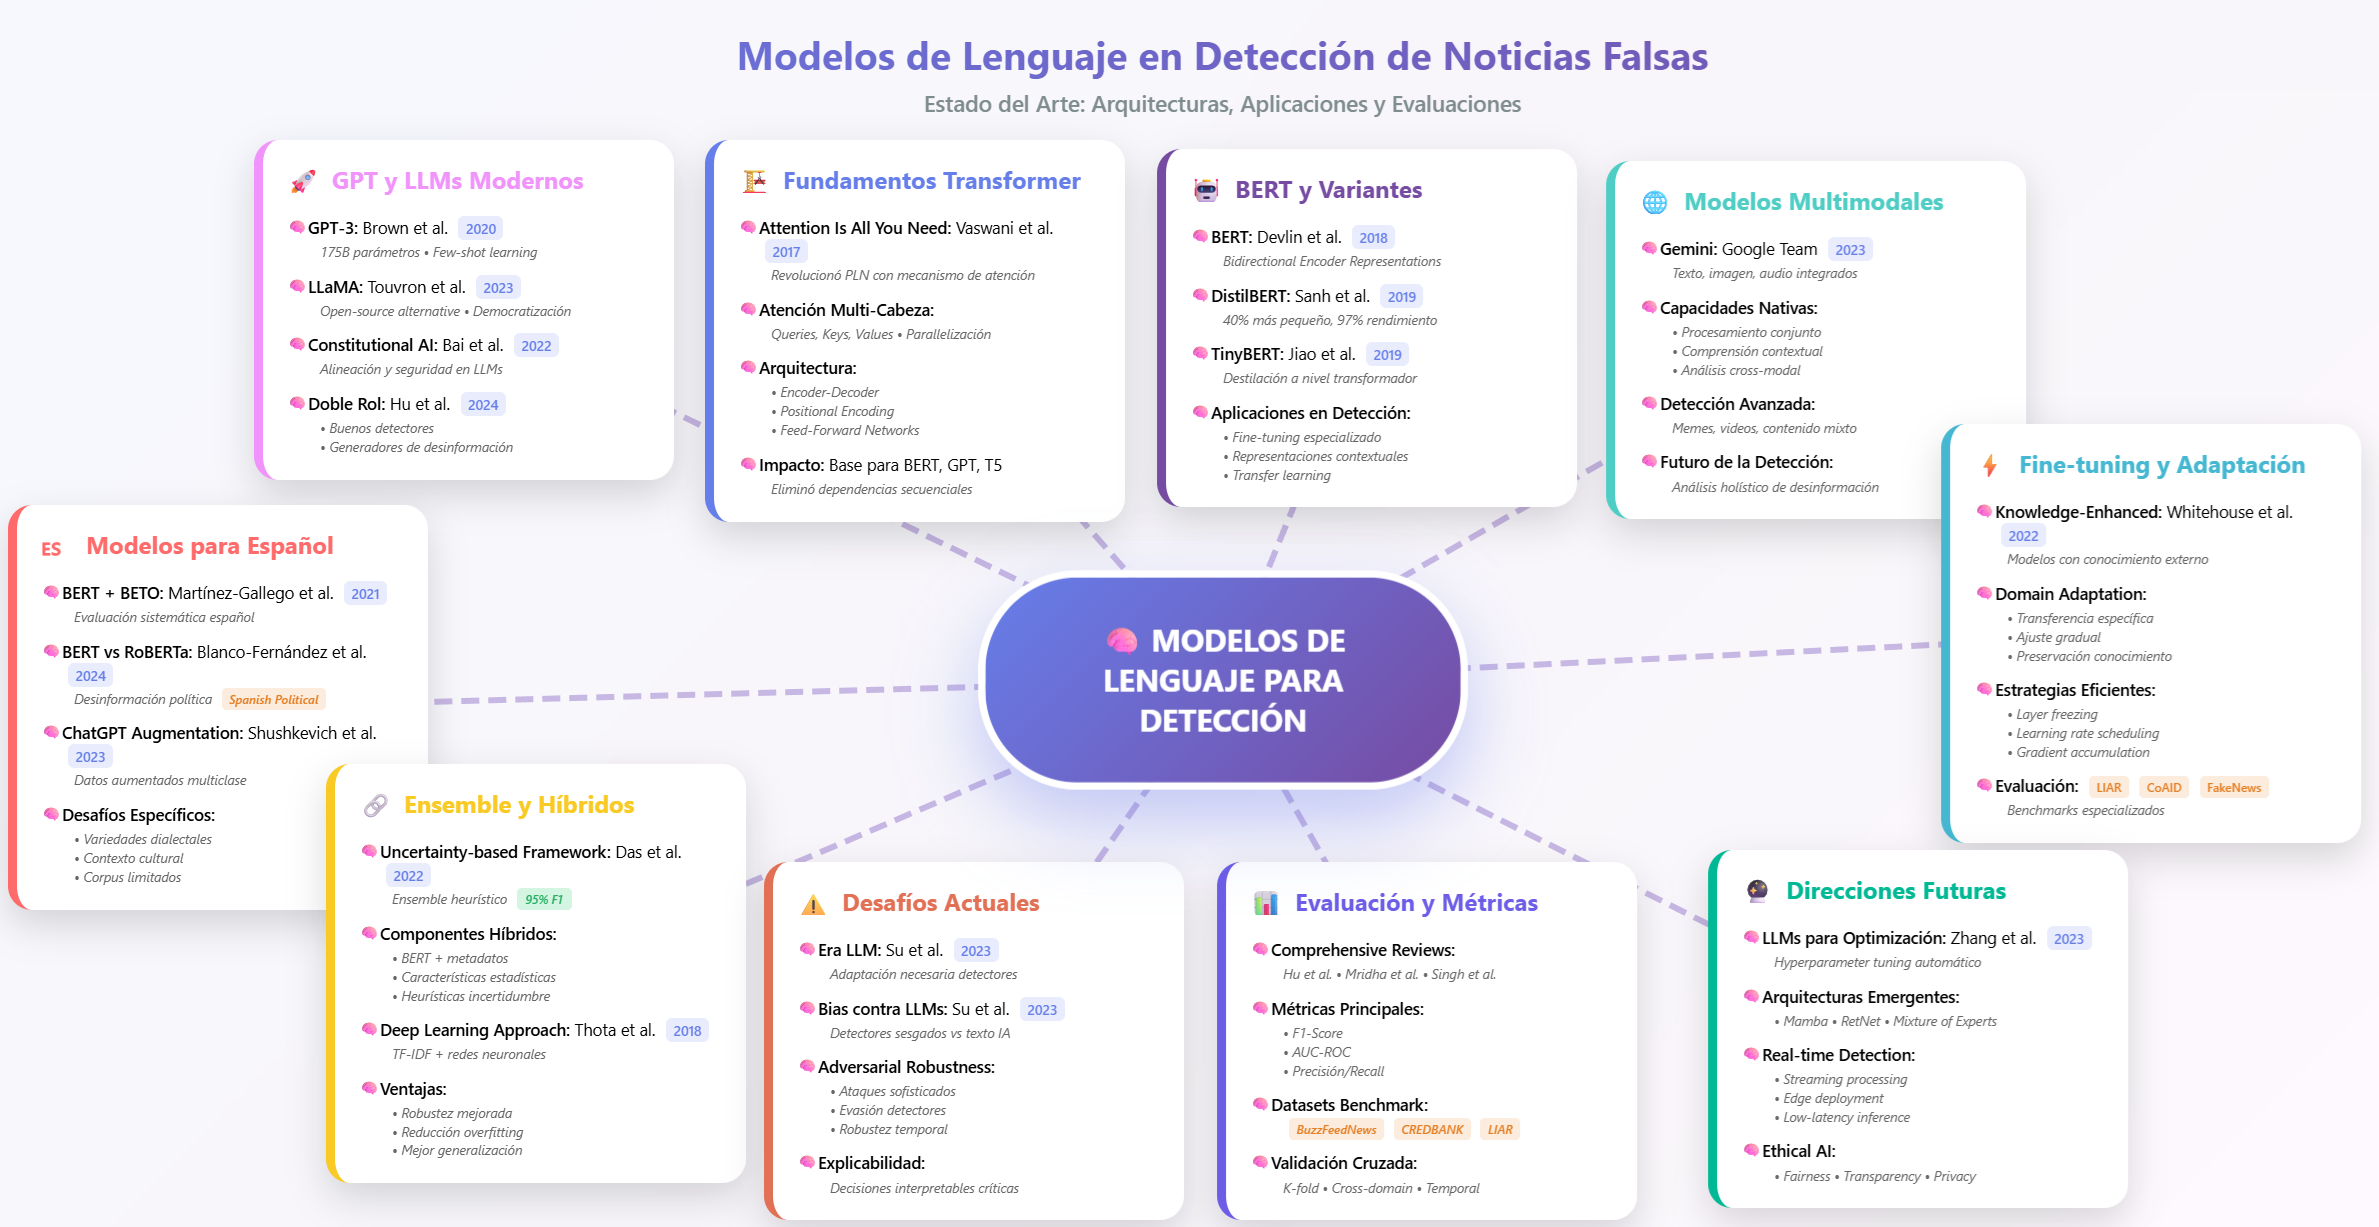
\includegraphics[width=\textwidth]{Imagenes/mapaConceptual3.png}
    \caption{Flujo del proceso de optimización metaheurística para detección de noticias falsas. Se muestra la transformación desde datos textuales hasta el modelo optimizado final, pasando por las etapas de preprocesamiento, optimización y evaluación.}
    \label{fig:flujo_metaheuristicas}
\end{figure}

Este flujo garantiza:
\begin{itemize}
    \item \textbf{Reproducibilidad:} Cada etapa está claramente definida con parámetros específicos
    \item \textbf{Escalabilidad:} El proceso puede aplicarse a corpus de diferentes tamaños
    \item \textbf{Transferibilidad:} La metodología es aplicable a otros problemas de clasificación textual
    \item \textbf{Transparencia:} Cada decisión algorítmica está justificada y documentada
\end{itemize}

\subsubsection{Consideraciones de Implementación}

\textbf{Manejo de Memoria:}
\begin{itemize}
    \item Uso de matrices dispersas (scipy.sparse) para representaciones TF-IDF
    \item Liberación explícita de memoria entre evaluaciones
    \item Procesamiento por lotes para corpus grandes
\end{itemize}

\textbf{Paralelización:}
\begin{itemize}
    \item Evaluación paralela de individuos en GA
    \item Vectorización de operaciones en PSO
    \item Múltiples arranques independientes en SA
\end{itemize}

\textbf{Validación y Robustez:}
\begin{itemize}
    \item Validación cruzada estratificada para preservar distribución de clases
    \item Múltiples ejecuciones independientes para análisis estadístico
    \item Manejo de casos extremos y configuraciones inválidas
\end{itemize}

\subsubsection{Métricas de Monitoreo del Proceso}

Durante la ejecución de cada algoritmo metaheurístico, se monitorizan las siguientes métricas:

\begin{enumerate}
    \item \textbf{Convergencia:} Evolución del mejor fitness a lo largo de las iteraciones
    \item \textbf{Diversidad:} Medida de dispersión en la población/enjambre
    \item \textbf{Estagnación:} Número de iteraciones sin mejora significativa
    \item \textbf{Eficiencia:} Número de evaluaciones para alcanzar convergencia
    \item \textbf{Estabilidad:} Variabilidad entre ejecuciones independientes
\end{enumerate}

Estas métricas permiten:
\begin{itemize}
    \item Ajustar parámetros de los algoritmos dinámicamente
    \item Detectar convergencia prematura o estagnación
    \item Comparar objetivamente el rendimiento de diferentes metaheurísticas
    \item Identificar configuraciones problemáticas o excepcionales
\end{itemize}

\subsection{Aplicaciones en Detección de Noticias Falsas}

\subsubsection{Modelado como Problema de Scheduling}

Aqil y Lahby \cite{aqil2021modeling} propusieron una perspectiva innovadora, modelando la detección de noticias falsas como un problema de Job Shop Scheduling. Compararon tres metaheurísticas:
\begin{itemize}
    \item \textbf{Algoritmo Genético (GA):} Evolución de soluciones mediante selección, cruce y mutación
    \item \textbf{Optimización por Enjambre de Partículas (PSO):} Búsqueda inspirada en comportamiento de bandadas
    \item \textbf{Colonia de Abejas Artificiales (ABC):} Algoritmo basado en comportamiento de forrajeo de abejas
\end{itemize}

Sus resultados mostraron que el algoritmo Iterated Greedy (IG) superó a las metaheurísticas bioinspiradas en este contexto específico.

\subsubsection{Optimización de Hiperparámetros en Deep Learning}

Bacanin et al. \cite{bacanin2023benefits} demostraron los beneficios de usar metaheurísticas para la calibración de hiperparámetros en modelos de deep learning. Su investigación mostró mejoras significativas sobre métodos tradicionales como grid search y random search:

\begin{itemize}
    \item \textbf{Eficiencia computacional:} Exploración más inteligente del espacio de hiperparámetros
    \item \textbf{Evitación de óptimos locales:} Capacidad de escape de configuraciones subóptimas
    \item \textbf{Adaptabilidad:} Ajuste dinámico según el comportamiento del modelo
\end{itemize}

La investigación que publiqué en \cite{hurtado2024calibracion} específicamente aborda la calibración de hiperparámetros en algoritmos metaheurísticos para detección de noticias falsas (como caso específico de fraude digital), proporcionando un marco metodológico relevante para esta tesis.

\subsubsection{Frameworks de Ensemble Heurístico}

Das et al. \cite{das2022heuristic} desarrollaron un marco de ensemble que combina:
\begin{itemize}
    \item \textbf{Modelos pre-entrenados:} BERT y similares para captura semántica
    \item \textbf{Características estadísticas:} Metadatos como URL, autor, timestamp
    \item \textbf{Heurísticas de incertidumbre:} Medidas de confianza para ponderación de predictores
\end{itemize}

Este enfoque híbrido logró F1-scores superiores al 95% en conjuntos de datos de referencia.

\subsection{Metaheurísticas para Detección de Fraude Financiero}

\subsubsection{Optimización Multi-objetivo}

Hidayattullah et al. \cite{hidayattullah2020financial} aplicaron metaheurísticas para optimizar la detección de fraude en estados financieros. Su enfoque multi-objetivo consideró:
\begin{itemize}
    \item \textbf{Precisión de clasificación:} Maximización de métricas de rendimiento
    \item \textbf{Eficiencia computacional:} Minimización de tiempo de entrenamiento
    \item \textbf{Robustez:} Estabilidad ante variaciones en los datos
\end{itemize}

Los resultados mostraron que SVM optimizado con Algoritmo Genético alcanzó 96.15\% de precisión, superando significativamente a métodos tradicionales.

\subsubsection{Optimización de Procesos Gaussianos}

Horak y Sabek \cite{horak2023gaussian} exploraron la optimización de hiperparámetros en Gaussian Process Regression para predicción de dificultades financieras. Su trabajo destaca la importancia de la calibración metaheurística en modelos probabilísticos.

\subsection{Algoritmos Híbridos Modernos}

\subsubsection{Enfoques Multi-thread}

Yildirim \cite{yildirim2023novel} propuso un enfoque metaheurístico híbrido multi-thread que optimiza simultáneamente:
\begin{itemize}
    \item Selección de características
    \item Parámetros del algoritmo de clasificación
    \item Arquitectura del ensemble
\end{itemize}

\subsubsection{PSO Adaptativo}

Deshai y Bhaskara Rao \cite{deshai2023unmasking} desarrollaron un enfoque CNN con PSO adaptativo para detectar reseñas falsas online. Su algoritmo PSO adaptativo ajusta dinámicamente los parámetros de velocidad e inercia basándose en el rendimiento de la iteración actual.

\section{Integración de Enfoques: Hacia Sistemas Híbridos}
\label{sec:integracion_enfoques}

\subsection{Combinación de Representaciones Clásicas y Modernas}

La tendencia actual en detección de noticias falsas favorece sistemas híbridos que combinan (principios aplicables a otros tipos de fraude digital):
\begin{itemize}
    \item \textbf{Características lingüísticas tradicionales:} TF-IDF, n-gramas, métricas de legibilidad
    \item \textbf{Embeddings contextuales:} Representaciones de BERT y similares
    \item \textbf{Metadatos estructurales:} Información temporal, de red social, y fuente
    \item \textbf{Características estilométricas:} Patrones de puntuación, longitud de oraciones, complejidad sintáctica
\end{itemize}

\subsection{Arquitecturas de Ensemble Optimizadas}

Las arquitecturas modernas emplean:
\begin{itemize}
    \item \textbf{Ensemble de modelos heterogéneos:} Combinación de clasificadores tradicionales y deep learning
    \item \textbf{Ponderación adaptativa:} Pesos dinámicos basados en confianza y rendimiento
    \item \textbf{Fusión de decisiones:} Estrategias sofisticadas para combinar predicciones múltiples
\end{itemize}

\subsection{Optimización End-to-End}

Zhang et al. \cite{zhang2023using} exploraron el uso de LLMs para optimización de hiperparámetros, abriendo nuevas posibilidades para la optimización automática de pipelines completos de detección.

\section{Desafíos y Direcciones Futuras}
\label{sec:desafios_direcciones}

\subsection{Desafíos Técnicos}

\begin{itemize}
    \item \textbf{Adaptación multilingüe:} Desarrollo de modelos robustos para múltiples idiomas
    \item \textbf{Detección en tiempo real:} Optimización para procesamiento de streams de alta velocidad
    \item \textbf{Robustez adversarial:} Resistencia a ataques de evasión sofisticados
    \item \textbf{Explicabilidad:} Desarrollo de modelos interpretables para decisiones críticas
\end{itemize}

\subsection{Consideraciones Éticas y Sociales}

\begin{itemize}
    \item \textbf{Sesgos algorítmicos:} Mitigación de discriminación en sistemas de detección
    \item \textbf{Privacidad:} Protección de datos personales en análisis de contenido
    \item \textbf{Transparencia:} Apertura en metodologías y criterios de detección
    \item \textbf{Impacto social:} Consideración de efectos en libertad de expresión y democracia
\end{itemize}

\section{Síntesis del Marco Teórico}
\label{sec:sintesis_marco}

Este marco teórico establece los fundamentos para las dos metodologías desarrolladas en esta tesis:

\begin{enumerate}
    \item \textbf{Enfoque Clásico Optimizado:} Utiliza representaciones TF-IDF con optimización metaheurística de hiperparámetros, proporcionando una línea base sólida y computacionalmente eficiente
    
    \item \textbf{Enfoque de Deep Learning:} Emplea modelos Transformer pre-entrenados con fine-tuning, aprovechando representaciones contextuales sofisticadas
\end{enumerate}

La combinación de ambos enfoques, sustentada en la literatura revisada, permite abordar el problema de detección de noticias falsas desde múltiples perspectivas, maximizando tanto la efectividad como la eficiencia computacional del sistema propuesto. La metodología desarrollada establece principios transferibles para abordar otros tipos de fraude digital con las adaptaciones correspondientes.

El marco establece también la base teórica para la contribución metodológica principal de esta tesis: la aplicación sistemática de técnicas metaheurísticas para la optimización de hiperparámetros en ambos paradigmas, desde clasificadores tradicionales hasta modelos de deep learning, en el contexto específico de textos en español.
\chapter{Estado del arte \label{cap:EstadoDelArte}}

La detección automatizada de noticias falsas ha emergido como una de las preocupaciones más apremiantes en la sociedad digital contemporánea, convirtiéndose en un campo de investigación multidisciplinario que abarca desde la ciencia de la computación hasta la psicología cognitiva. Durante la última década, investigadores de múltiples disciplinas han desarrollado enfoques innovadores que van desde técnicas tradicionales de procesamiento de lenguaje natural hasta modelos de lenguaje pre-entrenados de última generación, respondiendo a la creciente sofisticación de las campañas de desinformación y la velocidad sin precedentes con la que se propagan en las redes sociales.

En el contexto hispanohablante, esta problemática adquiere características particulares debido a las especificidades lingüísticas y culturales del español, incluyendo variaciones regionales, modismos locales, y patrones discursivos específicos que requieren enfoques metodológicos adaptados. La complejidad del español, con sus múltiples variantes geográficas y sus ricas estructuras sintácticas, presenta desafíos únicos para los sistemas automatizados de detección que tradicionalmente han sido desarrollados y entrenados principalmente en inglés.

Este capítulo examina las principales contribuciones científicas en el campo de la detección de desinformación, con especial énfasis en las aproximaciones que combinan técnicas de optimización metaheurística con modelos de aprendizaje automático. Se analiza también la evolución de los enfoques metodológicos, desde los primeros sistemas basados en características lingüísticas superficiales hasta los desarrollos más recientes que incorporan arquitecturas transformer y algoritmos de optimización bioinspirados, proporcionando las bases para entender tanto los avances logrados como los desafíos pendientes en este campo dinámico.

\section{Metodología de Búsqueda Bibliográfica}
\label{sec:busqueda_literatura}

Para garantizar una revisión lo más completa y actualizada posible de la literatura científica en el campo de la detección de noticias falsas, se diseñó una estrategia de búsqueda consultando múltiples bases de datos académicas reconocidas internacionalmente. El proceso de búsqueda se llevó a cabo entre agosto de 2023 y agosto de 2025, utilizando una combinación de términos clave específicos y operadores booleanos para maximizar la relevancia de los resultados.

Las bases de datos consultadas incluyeron repositorios académicos como Google Scholar, Semantic Scholar, Nature Digital Libraries, IOPscience, MDPI, Web of Science (WoS) y repositorios especializados como arXiv. La selección de estas fuentes se basó en su cobertura disciplinaria, calidad editorial, y relevancia específica para el campo de procesamiento de lenguaje natural y detección de desinformación. Adicionalmente, se incluyeron conferencias especializadas como ACL, EMNLP, y talleres específicos como CheckThat! para capturar los desarrollos más recientes en el área.

La búsqueda se estructuró en torno a combinaciones específicas de términos que reflejan las dimensiones principales de esta investigación, utilizando operadores booleanos para mejorar los resultados:

\begin{itemize}
    \item \textit{Spanish fake news detection} -- para capturar trabajos específicos del idioma español, incluyendo variaciones como ``detección de noticias falsas en español''
    \item \textit{Fake news detection language models} -- para incluir enfoques basados en modelos de lenguaje, cubriendo términos como BERT, RoBERTa, y transformer
    \item \textit{Metaheuristic hyperparameter optimization} -- para identificar aplicaciones de optimización metaheurística en aprendizaje automático
    \item \textit{Employment fraud detection} -- para abarcar el dominio del fraude laboral y su detección automatizada
    \item \textit{Simulated annealing fake news} y \textit{Genetic algorithm text classification} -- para enfoques específicos de optimización aplicados a clasificación textual
    \item \textit{Social media misinformation detection} -- para capturar trabajos enfocados en plataformas sociales
    \item \textit{Cross-lingual fake news} y \textit{multilingual misinformation} -- para incluir enfoques multilingües
\end{itemize}

El proceso de selección aplicó diferentes criterios de relevancia temática, calidad metodológica y actualidad temporal. Se priorizaron publicaciones de los últimos cinco años (2020-2025) sin excluir trabajos fundamentales para el campo que, aunque anteriores, establecieron bases teóricas o metodológicas esenciales. Los criterios de inclusión incluyeron: (1) contribuciones metodológicas originales, (2) validación empírica, (3) relevancia directa para la detección de desinformación, y (4) calidad de la revisión por pares. Los criterios de exclusión abarcaron: (1) trabajos puramente teóricos sin validación, (2) estudios con muestras insuficientes, (3) publicaciones en idiomas distintos al inglés o español, y (4) trabajos duplicados o versiones preliminares de conferencias posteriormente publicadas en revistas.

Como resultado de este proceso , se identificaron 80 trabajos que constituyen el núcleo de esta revisión, organizados temáticamente para facilitar el análisis comparativo y la identificación de tendencias emergentes en el campo.

\section{Panorama de la Investigación en Detección de Noticias Falsas}
\label{sec:panorama_investigacion}

El campo de la detección automatizada de desinformación ha experimentado una evolución notable y acelerada, caracterizada por una transición paradigmática desde enfoques tradicionales basados en características estadísticas simples hacia sistemas sofisticados que integran múltiples modalidades, técnicas de optimización avanzadas, y conocimiento contextual profundo. Esta evolución refleja tanto los avances tecnológicos en inteligencia artificial como la creciente sofisticación de las técnicas de desinformación empleadas por actores maliciosos.

La progresión temporal del campo puede dividirse en tres fases principales: (1) la era pioneera (2010-2016), caracterizada por enfoques basados en características lingüísticas superficiales y métodos de aprendizaje automático tradicionales; (2) la era de los modelos profundos (2017-2020), marcada por la adopción masiva de redes neuronales profundas y arquitecturas transformer; y (3) la era contemporánea (2021-presente), dominada por modelos de lenguaje de gran escala y enfoques híbridos que combinan múltiples técnicas de optimización.

\subsection{Fundamentos Metodológicos y Construcción de Corpus}

La disponibilidad de conjuntos de datos de alta calidad constituye el fundamento sobre el cual se construye cualquier sistema de detección eficaz, y representa uno de los mayores desafíos en el desarrollo de tecnologías de detección de desinformación. En el contexto hispanohablante, esta necesidad se vuelve particularmente crítica debido a la relativa escasez de recursos comparado con el inglés, donde la mayoría de la investigación se ha concentrado históricamente.

Los trabajos pioneros en esta dirección han establecido las bases metodológicas para la construcción y evaluación de corpus especializados, desarrollando protocolos de anotación, criterios de calidad, y marcos de evaluación que han influido significativamente en el desarrollo del campo. Acosta \cite{acosta2019construccion} desarrolló uno de los primeros marcos sistemáticos para la construcción de conjuntos de datos de noticias en español, estableciendo criterios rigurosos de calidad y protocolos de etiquetado manual que han influido significativamente en trabajos posteriores. Su metodología, centrada en la extracción automatizada seguida de verificación manual, demostró la viabilidad de crear recursos lingüísticos de gran escala para el español mientras mantenía estándares de calidad comparables a los corpus en inglés. El trabajo incluye un análisis detallado de las fuentes de noticias, criterios de selección temporal, y metodologías de validación cruzada entre anotadores.

El trabajo de Posadas-Durán et al. \cite{posadas2019detection} complementó estos esfuerzos al proponer un nuevo corpus específicamente diseñado para la detección de noticias falsas en español, incorporando características estilométricas innovadoras que capturan patrones lingüísticos sutiles pero significativos para la identificación de contenido desinformativo. Este enfoque pionero en el análisis del estilo de escritura como indicador de veracidad abrió nuevas líneas de investigación que han sido extensamente exploradas en trabajos posteriores. Su corpus incluye anotaciones multinivel que abarcan desde características superficiales del texto hasta análisis semánticos profundos, proporcionando un recurso invaluable para investigaciones subsequentes.

La comunidad científica internacional ha reconocido la importancia crítica de esta área a través de iniciativas competitivas sistemáticas que han proporcionado marcos estandarizados para la evaluación y comparación de sistemas. Los talleres CheckThat! organizados en el marco de CLEF \cite{alam2023overview, barron2023clef} han proporcionado marcos estandarizados para la evaluación comparativa de sistemas de detección, estableciendo métricas unificadas, protocolos de evaluación rigurosos, y conjuntos de datos de referencia que han contribuido significativamente a la maduración metodológica del campo. Estos talleres han evolucionado para incluir tareas cada vez más sofisticadas, desde la verificación de hechos básica hasta la detección de sesgo político y la evaluación de credibilidad en contenido multimodal.

\textbf{Un desafío fundamental en este campo es que no todos los corpus disponibles son equivalentes en términos de propósito, metodología de construcción, o calidad de anotación}. Esta heterogeneidad refleja la evolución natural del campo, donde diferentes grupos de investigación han abordado aspectos específicos del problema con enfoques metodológicos diversos. Algunos corpus se enfocan en análisis estilométrico, otros en detección política, y otros en evaluación de modelos específicos, lo que genera un ecosistema rico pero complejo de recursos disponibles.

En el contexto iberoamericano específicamente, las competiciones IberLEF han jugado un papel fundamental en el desarrollo de recursos y metodologías adaptadas a las particularidades del español. Aragón et al. \cite{aragon2020overview} documentaron los primeros esfuerzos sistemáticos para abordar la detección de noticias falsas en español mexicano, estableciendo metricas específicas para variantes regionales del idioma y desarrollando métricas de evaluación culturalmente sensibles. \textbf{Crucialmente, estos trabajos establecieron F1-Score como la métrica principal de comparación entre sistemas, junto con precisión y recall como métricas complementarias para análisis detallado del rendimiento}. Paralelamente, Gómez-Adorno et al. \cite{gomez2021overview} consolidaron estos esfuerzos en el marco de FakeDeS, estableciendo un referente duradero para la evaluación de sistemas en español que incluye tanto aspectos técnicos como consideraciones socioculturales.

\textbf{La estandarización de métricas de evaluación ha sido fundamental para el progreso del campo}. Los marcos CheckThat! \cite{barron2023clef} han establecido que las métricas fundamentales para clasificación binaria en detección de noticias falsas deben incluir: (1) \textit{Precisión} para medir la confiabilidad de las detecciones positivas, (2) \textit{Recall} (exhaustividad) para evaluar la cobertura de casos positivos reales, (3) \textit{F1-Score} como balance armónico entre ambas, y (4) \textit{Exactitud} para rendimiento general en datasets balanceados. Esta estandarización permite la comparación directa entre sistemas desarrollados por diferentes grupos de investigación y garantiza la reproducibilidad de los resultados.

La evolución hacia recursos más sofisticados se refleja en iniciativas recientes como el Spanish Fake News Corpus Version 2.0 \cite{ramirez2021spanish}, que incorpora anotaciones multinivel y metadatos enriquecidos que permiten análisis más profundos de los patrones de desinformación. Este corpus de segunda generación incluye información contextual sobre fuentes, temas, y patrones temporales de propagación, proporcionando un recurso muy valioso para la investigación en detección automatizada.

\begin{table}[htbp]
\centering
\adjustbox{width=\textwidth,center}{%
\small
\begin{tabular}{|l|l|l|c|c|}
\hline
\rowcolor{UAMPurple!20}
\textbf{Contribución Principal} & \textbf{Autores} & \textbf{Publicación} & \textbf{Año} & \textbf{Ref.} \\
\hline
\begin{tabular}[t]{@{}l@{}}Marco metodológico para construcción\\de conjuntos de datos de noticias en español\end{tabular} & Acosta, F. A. Z. & U. Politécnica de Madrid & 2019 & \cite{acosta2019construccion} \\
\hline
\begin{tabular}[t]{@{}l@{}}Evaluación multimodal y multigenre\\para verificación de contenido\end{tabular} & Alam, F., et al. & CEUR Workshop Proc. & 2023 & \cite{alam2023overview} \\
\hline
\begin{tabular}[t]{@{}l@{}}Análisis de agresividad y desinformación\\en español mexicano\end{tabular} & Aragón, M. E., et al. & IberLEF Workshop & 2020 & \cite{aragon2020overview} \\
\hline
\begin{tabular}[t]{@{}l@{}}Marco estandardizado CheckThat!\\para evaluación de sistemas\end{tabular} & Barrón-Cedeño, A., et al. & ECIR 2023 & 2023 & \cite{barron2023clef} \\
\hline
\begin{tabular}[t]{@{}l@{}}Consolidación de métricas FakeDeS\\para detección en español\end{tabular} & Gómez-Adorno, H., et al. & Procesamiento del Lenguaje Natural & 2021 & \cite{gomez2021overview} \\
\hline
\begin{tabular}[t]{@{}l@{}}Corpus pionero con características\\estilométricas para español\end{tabular} & Posadas-Durán, J. P., et al. & J. of Intelligent and Fuzzy Systems & 2019 & \cite{posadas2019detection} \\
\hline
\begin{tabular}[t]{@{}l@{}}Corpus enriquecido con anotaciones\\multinivel versión 2.0\end{tabular} & Ramírez Cruz, J. M., et al. & GitHub Repository & 2021 & \cite{ramirez2021spanish} \\
\hline
\begin{tabular}[t]{@{}l@{}}Técnicas de aprendizaje automático\\aplicadas al español\end{tabular} & Tretiakov, A., et al. & Springer & 2022 & \cite{tretiakov2022detection} \\
\hline
\end{tabular}
}
\caption{Contribuciones fundamentales en metodología y construcción de corpus para español.}
\label{tab:articulos_metodologia}
\end{table}

Esta base metodológica en constante evolución ha permitido el desarrollo de aproximaciones cada vez más sofisticadas que integran múltiples tipos de evidencia, técnicas de análisis avanzadas, y conocimiento contextual, estableciendo el terreno base para los desarrollos contemporáneos en modelos de lenguaje de gran escala y optimización metaheurística que se analizan en las siguientes secciones.

\subsection{Evolución de los Modelos de Lenguaje en Detección de Desinformación}

La irrupción de los modelos de lenguaje pre-entrenados ha revolucionado completamente el panorama de la detección automatizada de noticias falsas, representando un cambio paradigmático fundamental en cómo conceptualizamos y abordamos la comprensión automatizada de texto. Esta transformación se caracteriza por una progresión clara y acelerada desde arquitecturas básicas hacia sistemas cada vez más sofisticados que integran conocimiento contextual profundo, capacidades de razonamiento complejo, y comprensión semántica avanzada.

El punto de inflexión histórico llegó con la introducción de BERT \cite{devlin2018bert}, cuya arquitectura bidireccional revolucionaria permitió capturar dependencias contextuales de manera más efectiva que los enfoques secuenciales previos basados en LSTM o GRU. La capacidad fundamental de BERT para entender el contexto completo de una oración de manera simultánea, en lugar de procesarla secuencialmente de izquierda a derecha como los modelos anteriores, representó un avance fundamental que ha sido extensamente aplicado y adaptado en la detección de desinformación. Esta arquitectura bidireccional permite al modelo capturar relaciones complejas entre palabras que pueden estar distantes en el texto pero semánticamente relacionadas, una característica crucial para identificar inconsistencias sutiles y patrones desinformativos sofisticados.

La necesidad imperativa de modelos más eficientes computacionalmente, especialmente para aplicaciones en tiempo real y dispositivos con recursos limitados, llevó al desarrollo de variantes optimizadas como DistilBERT \cite{sanh2019distilbert}, que mantiene aproximadamente el $97\%$ del rendimiento de BERT con solo el $60\%$ de sus parámetros mediante técnicas innovadoras de destilación de conocimiento. Esta línea de investigación, que incluye también desarrollos como TinyBERT \cite{jiao2019tinybert}, ha demostrado ser crucial para aplicaciones prácticas de detección en tiempo real donde los recursos computacionales son limitados pero la precisión no puede comprometerse significativamente.

En el contexto específico y culturalmente relevante del español, el trabajo de Martínez-Gallego et al. \cite{martinez2021fake} exploró la aplicación de técnicas de aprendizaje profundo, incluyendo tanto BERT como BETO (la variante específicamente pre-entrenada en español), para la detección de noticias falsas. Sus resultados demostraron de manera convincente que los modelos específicamente pre-entrenados en español superan consistentemente a las versiones multilingües genéricas, subrayando la importancia de la especialización lingüística y cultural en el desarrollo de sistemas de detección efectivos. Este hallazgo tiene implicaciones profundas para el desarrollo de sistemas de detección en idiomas distintos al inglés.

Blanco-Fernández et al. \cite{blanco2024enhancing} extendieron significativamente esta línea de investigación al comparar sistemáticamente BERT y RoBERTa en tareas específicas de detección de desinformación en español, proporcionando evidencia empírica detallada sobre las ventajas relativas de diferentes arquitecturas transformer para este dominio específico. Su trabajo demostró que RoBERTa, con su entrenamiento más extenso y metodología de enmascaramiento optimizada, puede ofrecer mejoras significativas en la detección de patrones sutiles de desinformación, especialmente en textos que emplean técnicas de manipulación sofisticadas.

El surgimiento explosivo de modelos generativos de gran escala ha introducido dimensiones completamente nuevas y complejas al problema de detección. Brown et al. \cite{brown2020language} establecieron con GPT-3 las bases conceptuales y técnicas de los modelos de lenguaje de gran escala, cuyas capacidades avanzadas de generación de texto han complicado paradójicamente el problema de detección al crear contenido sintético cada vez más indistinguible del contenido humano auténtico. El equipo de Gemini \cite{gemini2023family} ha continuado esta evolución hacia modelos multimodales que pueden procesar y generar simultáneamente texto, imágenes y otros tipos de información, ampliando el alcance y la complejidad de los desafíos de detección.

Esta evolución acelerada ha generado nuevos desafíos metodológicos y éticos que requieren enfoques innovadores. Su et al. \cite{su2023adapting} analizaron cómo la era de los modelos de lenguaje grandes requiere adaptaciones fundamentales en las técnicas de detección tradicionales, incluyendo nuevos marcos teóricos y metodológicos para abordar contenido generado artificialmente. Complementariamente, en otro de sus trabajos \cite{su2023fake} reveló que los detectores existentes muestran sesgos sistemáticos significativos contra texto generado por LLMs, planteando cuestiones fundamentales sobre la generalización, robustez, y equidad de los sistemas de detección contemporáneos.

El enfoque hacia la mejora continua y la adaptación de estos sistemas se refleja en trabajos innovadores como el de Shushkevich et al. \cite{shushkevich2023improving}, que exploraron la combinación sinérgica de modelos BERT con datos aumentados mediante ChatGPT, demostrando cómo los propios LLMs pueden utilizarse estratégicamente para mejorar la detección de contenido falso mediante técnicas de augmentación de datos y transferencia de conocimiento.

Una perspectiva particularmente interesante e importante emerge del trabajo de Hu et al. \cite{hu2024bad}, que examina el papel dual y paradójico de los modelos de lenguaje grandes como potenciales generadores de desinformación y, simultáneamente, como herramientas para su detección. Esta dualidad fundamental refleja la complejidad creciente del panorama tecnológico actual y plantea cuestiones éticas y prácticas importantes sobre el desarrollo responsable de tecnologías de IA.

\begin{table}[htbp]
\centering
\adjustbox{width=\textwidth,center}{%
\small
\begin{tabular}{|l|l|l|c|c|}
\hline
\rowcolor{UAMPurple!20}
\textbf{Innovación Principal} & \textbf{Autores} & \textbf{Publicación} & \textbf{Año} & \textbf{Ref.} \\
\hline
\begin{tabular}[t]{@{}l@{}}Arquitectura bidireccional para\\comprensión contextual profunda\end{tabular} & Devlin, J., et al. & arXiv & 2018 & \cite{devlin2018bert} \\
\hline
\begin{tabular}[t]{@{}l@{}}Destilación de conocimiento para\\modelos eficientes\end{tabular} & Sanh, V., et al. & arXiv & 2019 & \cite{sanh2019distilbert} \\
\hline
\begin{tabular}[t]{@{}l@{}}Optimización extrema con\\TinyBERT\end{tabular} & Jiao, X., et al. & arXiv & 2019 & \cite{jiao2019tinybert} \\
\hline
\begin{tabular}[t]{@{}l@{}}Aplicación sistemática de transformers\\en español\end{tabular} & Martínez-Gallego, K., et al. & arXiv & 2021 & \cite{martinez2021fake} \\
\hline
\begin{tabular}[t]{@{}l@{}}Comparación BERT vs RoBERTa\\para español\end{tabular} & Blanco-Fernández, Y., et al. & Applied Sciences & 2024 & \cite{blanco2024enhancing} \\
\hline
\begin{tabular}[t]{@{}l@{}}Capacidades emergentes en\\modelos de gran escala\end{tabular} & Brown, T. B., et al. & arXiv & 2020 & \cite{brown2020language} \\
\hline
\begin{tabular}[t]{@{}l@{}}Modelos multimodales de\\próxima generación\end{tabular} & Gemini Team, Google & arXiv & 2023 & \cite{gemini2023family} \\
\hline
\begin{tabular}[t]{@{}l@{}}Adaptación para la era\\de LLMs\end{tabular} & Su, J., et al. & arXiv & 2023 & \cite{su2023adapting} \\
\hline
\end{tabular}
}
\caption{Evolución de modelos de lenguaje aplicados a detección de desinformación.}
\label{tab:modelos_lenguaje}
\end{table}

\subsection{Técnicas de Optimización Metaheurística en Detección de Desinformación}

La aplicación de algoritmos metaheurísticos a la detección de noticias falsas representa una forma innovadora entre dos áreas de investigación que han madurado de manera independiente pero complementaria durante las últimas décadas. Por un lado, las metaheurísticas han demostrado repetidamente su eficacia excepcional en la resolución de problemas de optimización complejos, no lineales, y multimodales en múltiples dominios científicos y de ingeniería. Por otro lado, la detección de desinformación enfrenta desafíos inherentes y crecientes de optimización, particularmente en la calibración precisa de hiperparámetros, la selección inteligente de características relevantes, y la optimización de arquitecturas de modelos complejos.

Una aproximación innovadora consiste en formular la detección de noticias falsas como un problema de optimización combinatorial. Esta perspectiva tiene ventajas tanto teóricas como prácticas, ya que permite aplicar décadas de investigación en optimización metaheurística a un problema social actual y relevante. 

Aqil y Lahby \cite{aqil2021modeling} fueron pioneros en modelar esta tarea como un problema de planificación de tareas (Job Shop Scheduling). En su enfoque, diferentes algoritmos de procesamiento de texto deben ejecutarse de manera óptima considerando restricciones de tiempo, recursos computacionales y calidad de resultados. Los autores evaluaron tres metaheurísticas principales: Iterated Greedy, Algoritmos Genéticos y Artificial Bee Colony. Sus resultados mostraron que Iterated Greedy superaba consistentemente a las otras alternativas tanto en eficiencia computacional como en calidad de soluciones, estableciendo un precedente metodológico importante para investigaciones posteriores.

En el ámbito específico y técnicamente desafiante de la detección de reseñas falsas, que comparte muchas características con la detección de noticias falsas, Deshai y Rao \cite{deshai2023unmasking} desarrollaron un enfoque innovador y técnicamente sofisticado que combina redes neuronales convolucionales (CNN) con Optimización por Enjambre de Partículas adaptativo (PSO). Su contribución principal radica en la demostración empírica y teórica de que PSO puede optimizar efectivamente los hiperparámetros complejos de redes CNN, superando métodos tradicionales como Grid Search y Random Search en términos de eficiencia computacional, convergencia, y calidad de resultados finales. El trabajo incluye un análisis detallado de la superficie de respuesta del espacio de hiperparámetros y demuestra cómo PSO puede navegar eficientemente estos espacios multidimensionales complejos.

Bacanin et al. \cite{bacanin2023benefits} investigaron la aplicación de metaheurísticas para optimizar hiperparámetros en modelos de aprendizaje profundo, enfocándose originalmente en predicción de cargas energéticas. Sus resultados con Algoritmos Genéticos Binarios, PSO y Recocido Simulado para modelos LSTM demuestran mejoras consistentes sobre métodos tradicionales de optimización. El trabajo presenta comparaciones rigurosas con técnicas baseline y análisis estadísticos que validan la efectividad de estas aproximaciones metaheurísticas, ofreciendo insights valiosos que se extienden más allá del dominio energético hacia aplicaciones de procesamiento de texto y análisis de sentimientos.

Das et al. \cite{das2022heuristic} desarrollaron un marco de trabajo basado en técnicas heurísticas para manejar la incertidumbre en la clasificación de tweets y artículos de noticias. Su enfoque reconoce que la detección de desinformación requiere el manejo sofisticado de múltiples fuentes de evidencia y contextos sociales complejos, más allá de la clasificación binaria tradicional. El marco de trabajo incluye mecanismos para cuantificar y propagar incertidumbre a través de las diferentes etapas del pipeline de detección.

Yildirim \cite{yildirim2023novel} propuso un enfoque multi-hilo que combina múltiples metaheurísticas para la detección multimodal de noticias falsas. Esta aproximación reconoce que los sistemas de desinformación contemporáneos integran múltiples modalidades (texto, imágenes, videos, metadatos) que requieren estrategias de optimización coordinadas para lograr detección efectiva.

\begin{table}[htbp]
\centering
\adjustbox{width=\textwidth,center}{%
\small
\begin{tabular}{|l|l|l|c|c|}
\hline
\rowcolor{UAMPurple!20}
\textbf{Contribución Metodológica} & \textbf{Autores} & \textbf{Publicación} & \textbf{Año} & \textbf{Ref.} \\
\hline
\begin{tabular}[t]{@{}l@{}}Formulación como problema de\\planificación de tareas\end{tabular} & Aqil, S., \& Lahby, M. & Studies in Comp. Intelligence & 2021 & \cite{aqil2021modeling} \\
\hline
\begin{tabular}[t]{@{}l@{}}PSO adaptativo para optimización\\de CNN en detección de reseñas\end{tabular} & Deshai, N., \& Rao, B. B. & Soft Computing & 2023 & \cite{deshai2023unmasking} \\
\hline
\begin{tabular}[t]{@{}l@{}}Evidencia sistemática de beneficios\\en modelos de aprendizaje profundo\end{tabular} & Bacanin, N., et al. & Energies & 2023 & \cite{bacanin2023benefits} \\
\hline
\begin{tabular}[t]{@{}l@{}}Marco ensemble para manejo\\de incertidumbre\end{tabular} & Das, S. D., et al. & Neurocomputing & 2022 & \cite{das2022heuristic} \\
\hline
\begin{tabular}[t]{@{}l@{}}Aplicación específica para\\español y fraude digital\end{tabular} & Hurtado Avilés, G., et al. & BUAP & 2024 & \cite{hurtado2024calibracion} \\
\hline
\begin{tabular}[t]{@{}l@{}}Enfoque multi-hilo para\\detección multimodal\end{tabular} & Yildirim, G. & Applied Intelligence & 2023 & \cite{yildirim2023novel} \\
\hline
\begin{tabular}[t]{@{}l@{}}Combinación K-Means y SVM\\para selección de características\end{tabular} & Yazdi, K. M., et al. & WASET & 2020 & \cite{yazdi2020improving} \\
\hline
\begin{tabular}[t]{@{}l@{}}Optimización de ensemble\\con metaheurísticas\end{tabular} & Yasmin, A., et al. & PLOS ONE & 2024 & \cite{yasmin2024ensemble} \\
\hline
\end{tabular}
}
\caption{Contribuciones metodológicas en optimización metaheurística para detección.}
\label{tab:articulos_metaheuristicas}
\end{table}

La diversificación creciente hacia enfoques híbridos se observa claramente en estudios metodológicamente innovadores como el de Yazdi et al. \cite{yazdi2020improving}, que combina técnicas de clustering K-Means con máquinas de vectores de soporte (SVM) para optimizar la selección de características en espacios de alta dimensionalidad. Su contribución demuestra que la integración inteligente de metaheurísticas con técnicas de preprocesamiento puede mejorar significativamente la eficacia de detectores convencionales, especialmente en escenarios donde la dimensionalidad de los datos presenta desafíos computacionales significativos.

Finalmente, el trabajo de Yasmin et al. \cite{yasmin2024ensemble} avanza decididamente hacia la optimización completa y sistemática de sistemas ensemble, donde múltiples metaheurísticas colaboran de manera coordinada en la calibración simultánea de pesos, hiperparámetros, y arquitecturas de diferentes clasificadores base. Este enfoque representa la frontera actual más avanzada en la aplicación de optimización metaheurística a problemas de detección complejos y establece precedentes importantes para desarrollos futuros en el campo.

\section{Algoritmos Metaheurísticos: Fundamentos Teóricos y Aplicaciones Prácticas}
\label{sec:algoritmos_metaheuristicos}

Los algoritmos metaheurísticos representan una clase fundamental y versátil de técnicas de optimización que han demostrado ser especialmente efectivas para resolver problemas complejos de optimización no lineal, no convexos, y multimodales, incluyendo específicamente la calibración de hiperparámetros en modelos de aprendizaje automático y la optimización de arquitecturas de redes neuronales. Esta sección presenta los fundamentos teóricos, principios operativos, y aplicaciones prácticas de los principales algoritmos metaheurísticos utilizados en la detección de noticias falsas y optimización de modelos.

\subsection{Algoritmos Genéticos (GA): Evolución Artificial para Optimización}

Los Algoritmos Genéticos, introducidos por Holland \cite{holland1992adaptation} en su investigación original sobre adaptación en sistemas naturales y artificiales, están inspirados profundamente en la teoría de la evolución de Darwin y los principios fundamentales de la genética molecular. Estos algoritmos mantienen una población diversa de soluciones candidatas que evolucionan iterativamente a través de operadores genéticos cuidadosamente diseñados como selección, cruzamiento (crossover), y mutación, replicando los procesos evolutivos naturales pero aplicados a espacios de soluciones abstractos.

El trabajo fundamental de Holland estableció no solo las bases teóricas para esta clase de algoritmos bioinspirados, sino también demostraciones formales de su capacidad para explorar eficientemente espacios de búsqueda complejos y multimodales mediante un balance inteligente entre exploración (búsqueda global) y explotación (refinamiento local). La teoría de los esquemas (schema theory) desarrollada por Holland proporciona fundamentos matemáticos sólidos para entender cómo estos algoritmos pueden converger hacia regiones óptimas del espacio de búsqueda.

El funcionamiento básico de los algoritmos genéticos involucra una secuencia iterativa de operaciones: (1) evaluación de la aptitud (fitness) de cada individuo en la población usando una función objetivo específica del problema, (2) selección probabilística de los mejores candidatos para reproducción basada en su fitness relativo, (3) generación de nuevas soluciones mediante operadores de cruzamiento que combinan información genética de padres seleccionados, y (4) aplicación de mutación para introducir diversidad genética y evitar convergencia prematura. Este proceso iterativo permite la convergencia gradual hacia soluciones óptimas o cercanas al óptimo global.

En el contexto específico de la detección de noticias falsas, los algoritmos genéticos han demostrado particular efectividad en la optimización simultánea de múltiples hiperparámetros de modelos complejos, la selección automática de características relevantes desde espacios de alta dimensionalidad, y la evolución de arquitecturas de redes neuronales que maximizan el rendimiento de detección.

\subsection{Optimización por Enjambre de Partículas (PSO): Inteligencia Colectiva}

La Optimización por Enjambre de Partículas fue desarrollada independientemente por Kennedy y Eberhart \cite{kennedy1995particle}, inspirándose en observaciones detalladas del comportamiento social emergente de bandadas de pájaros, bancos de peces, y otros sistemas biológicos que exhiben inteligencia colectiva. Una formulación alternativa pero complementaria fue presentada por Eberhart y Kennedy \cite{eberhart1995particle} en el mismo período, consolidando esta técnica como una de las metaheurísticas más utilizadas y estudiadas en optimización global.

En PSO, cada partícula individual representa una solución potencial completa que se mueve dinámicamente a través del espacio de búsqueda multidimensional siguiendo una combinación ponderada de su propia experiencia histórica (mejor posición personal encontrada, pbest) y la experiencia colectiva del enjambre (mejor posición global encontrada por cualquier partícula, gbest). La velocidad y posición de cada partícula se actualizan dinámicamente en cada iteración usando ecuaciones de movimiento que incorporan componentes de inercia, atracción cognitiva (hacia pbest), y atracción social (hacia gbest).

Esta formulación matemática permite un equilibrio natural entre exploración y explotación del espacio de soluciones: la inercia mantiene la dirección de búsqueda previa, la atracción cognitiva favorece la explotación de regiones prometedoras encontradas por cada partícula, y la atracción social facilita el intercambio de información entre partículas y la convergencia hacia regiones globalmente prometedoras.

En aplicaciones de detección de desinformación, PSO ha demostrado particular efectividad en la calibración de hiperparámetros de redes neuronales convolucionales y transformers, donde el espacio de búsqueda es continuo y las evaluaciones de aptitud son computacionalmente costosas.

\subsection{Recocido Simulado: Física Estadística para Optimización}

El Recocido Simulado, propuesto originalmente por Kirkpatrick, Gelatt y Vecchi \cite{kirkpatrick1983optimization}, se basa en el proceso físico de enfriamiento controlado de metales (annealing) utilizado en metalurgia para obtener estructuras cristalinas de mínima energía. Este algoritmo permite escapar inteligentemente de óptimos locales mediante la aceptación probabilística de soluciones temporalmente peores, con una probabilidad que disminuye gradualmente según un esquema de enfriamiento cuidadosamente diseñado.

La analogía con la física estadística es profunda: la función objetivo corresponde a la energía del sistema, la variable de control (temperatura) determina la probabilidad de aceptar soluciones subóptimas, y el esquema de enfriamiento dicta cómo esta probabilidad decrece a lo largo del tiempo. La aceptación probabilística se basa en la distribución de Boltzmann, permitiendo que el algoritmo escape de mínimos locales cuando la temperatura es alta y converja hacia soluciones de alta calidad cuando la temperatura es baja.

Los métodos Multi-arranque, formalizados por Martí, Resende y Pardalos \cite{marti2018multistart}, consisten en ejecutar múltiples corridas independientes de un algoritmo de búsqueda local desde diferentes puntos de inicio cuidadosamente seleccionados. La combinación de Recocido Simulado con estrategias Multi-arranque (MSA) permite aprovechar sinérgicamente las ventajas de ambos enfoques: la capacidad de escape de óptimos locales del primero y la diversificación exhaustiva del espacio de búsqueda del segundo.

\subsection{Búsqueda Dispersa (Scatter Search): Combinación Determinística}

La Búsqueda Dispersa, desarrollada por Glover \cite{glover1998template} como parte de su marco más amplio de metaheurísticas basadas en memoria, utiliza estrategias sistemáticas y determinísticas para combinar soluciones de referencia de alta calidad y generar nuevas soluciones prometedoras. A diferencia de otros métodos que dependen predominantemente de procesos aleatorios, SS emplea combinaciones determinísticas cuidadosamente diseñadas y diversificación controlada basada en medidas de distancia en el espacio de soluciones.

El algoritmo mantiene un conjunto pequeño pero diverso de soluciones de referencia de alta calidad, utilizando métodos de combinación específicos del problema para generar nuevas soluciones candidatas. La selección de soluciones de referencia se basa en criterios que balancean calidad (fitness) y diversidad (distancia en el espacio de soluciones), asegurando que el conjunto de referencia capture diferentes regiones prometedoras del espacio de búsqueda.

Esta aproximación ha demostrado ser particularmente efectiva en problemas de optimización combinatorial donde la estructura del problema permite el diseño de operadores de combinación inteligentes que preservan características deseables de las soluciones padre.

\subsection{Búsqueda en Vecindades Variables (VNS): Exploración Sistemática}

La Búsqueda en Vecindades Variables, introducida por Mladenović y Hansen \cite{mladenovic1997variable}, se basa en el principio fundamental de cambio sistemático de estructuras de vecindad durante el proceso de búsqueda local. Esta técnica es especialmente efectiva para escapar de óptimos locales explorando diferentes definiciones de vecindad que capturan aspectos diversos de la estructura del problema.

VNS alterna sistemáticamente entre fases de diversificación (mediante la exploración de vecindades más amplias que permiten movimientos grandes en el espacio de soluciones) y intensificación (búsqueda local en vecindades más restringidas que refinan soluciones prometedoras), proporcionando un marco flexible y adaptable para la optimización que puede personalizarse a diferentes tipos de problemas y estructuras de espacio de búsqueda.

El principio central de VNS es que diferentes estructuras de vecindad proporcionan diferentes perspectivas del paisaje de optimización, y que el cambio sistemático entre estas perspectivas puede revelar regiones prometedoras que permanecerían ocultas usando una sola definición de vecindad.

\begin{table}[htbp]
\centering
\adjustbox{width=\textwidth,center}{%
\small
\begin{tabular}{|l|l|l|l|c|}
\hline
\rowcolor{UAMPurple!20}
\textbf{Algoritmo} & \textbf{Inspiración} & \textbf{Características Principales} & \textbf{Aplicaciones en Detección} & \textbf{Ref.} \\
\hline
\begin{tabular}[t]{@{}l@{}}Algoritmos Genéticos\\(GA)\end{tabular} & \begin{tabular}[t]{@{}l@{}}Evolución biológica\\y genética molecular\end{tabular} & \begin{tabular}[t]{@{}l@{}}Población de soluciones,\\operadores genéticos,\\selección natural,\\teoría de esquemas\end{tabular} & \begin{tabular}[t]{@{}l@{}}Optimización de hiperparámetros,\\selección de características,\\evolución de arquitecturas\\de redes neuronales\end{tabular} & \cite{holland1992adaptation} \\
\hline
\begin{tabular}[t]{@{}l@{}}Optimización por\\Enjambre de Partículas\\(PSO)\end{tabular} & \begin{tabular}[t]{@{}l@{}}Comportamiento\\social de bandadas\\y enjambres\end{tabular} & \begin{tabular}[t]{@{}l@{}}Partículas con velocidad\\y posición, memoria\\personal y social,\\inteligencia colectiva\end{tabular} & \begin{tabular}[t]{@{}l@{}}Calibración de pesos en redes,\\optimización de parámetros\\de modelos de lenguaje,\\ajuste de transformers\end{tabular} & \cite{kennedy1995particle} \\
\hline
\begin{tabular}[t]{@{}l@{}}Recocido Simulado\\(SA)\end{tabular} & \begin{tabular}[t]{@{}l@{}}Proceso físico de\\enfriamiento de metales\\y mecánica estadística\end{tabular} & \begin{tabular}[t]{@{}l@{}}Aceptación probabilística,\\esquema de enfriamiento,\\escape de óptimos locales,\\distribución de Boltzmann\end{tabular} & \begin{tabular}[t]{@{}l@{}}Optimización de arquitecturas\\profundas, ajuste fino\\de modelos complejos,\\calibración no convexa\end{tabular} & \cite{kirkpatrick1983optimization} \\
\hline
\begin{tabular}[t]{@{}l@{}}Multi-arranque\\(Multi-start)\end{tabular} & \begin{tabular}[t]{@{}l@{}}Diversificación\\de puntos de inicio\\y exploración global\end{tabular} & \begin{tabular}[t]{@{}l@{}}Múltiples ejecuciones\\independientes, exploración\\global del espacio,\\robustez estadística\end{tabular} & \begin{tabular}[t]{@{}l@{}}Inicialización robusta\\de modelos, validación\\cruzada optimizada,\\ensemble de optimizadores\end{tabular} & \cite{marti2018multistart} \\
\hline
\begin{tabular}[t]{@{}l@{}}Búsqueda Dispersa\\(SS)\end{tabular} & \begin{tabular}[t]{@{}l@{}}Combinación sistemática\\de soluciones diversas\\y métodos determinísticos\end{tabular} & \begin{tabular}[t]{@{}l@{}}Conjunto de referencia,\\combinaciones determinísticas,\\diversificación controlada,\\memoria adaptativa\end{tabular} & \begin{tabular}[t]{@{}l@{}}Ensemble de modelos,\\combinación de características,\\optimización de pipelines,\\fusión de arquitecturas\end{tabular} & \cite{glover1998template} \\
\hline
\begin{tabular}[t]{@{}l@{}}Búsqueda en Vecindades\\Variables (VNS)\end{tabular} & \begin{tabular}[t]{@{}l@{}}Cambio sistemático\\de estructuras de\\vecindad y perspectivas\\múltiples\end{tabular} & \begin{tabular}[t]{@{}l@{}}Múltiples definiciones\\de vecindad, alternancia\\entre diversificación\\e intensificación\end{tabular} & \begin{tabular}[t]{@{}l@{}}Exploración de espacios\\de hiperparámetros,\\optimización de topologías\\de red, búsqueda adaptativa\end{tabular} & \cite{mladenovic1997variable} \\
\hline
\end{tabular}
}
\caption{Algoritmos metaheurísticos: características fundamentales y aplicaciones en detección de noticias falsas.}
\label{tab:algoritmos_metaheuristicos}
\end{table}

Estos algoritmos han demostrado ser especialmente valiosos en el contexto complejo y multifacético de la detección de noticias falsas, donde los espacios de búsqueda de hiperparámetros son intrínsecamente complejos, multidimensionales, y frecuentemente multimodales. Su capacidad probada para balancear exploración y explotación los convierte en herramientas ideales para optimizar el rendimiento de modelos de aprendizaje automático en tareas de clasificación textual, especialmente cuando se enfrentan a conjuntos de datos desbalanceados, ruidosos, o de alta dimensionalidad que son característicos en aplicaciones de detección de desinformación.

\section{Hiperparámetros en Modelos de Aprendizaje Automático: Fundamentos y Optimización}
\label{sec:hiperparametros}

\subsection{Naturaleza y Definición de Hiperparámetros}

Para explicar este concepto fundamental de manera accesible pero técnicamente precisa, utilizaremos una analogía culinaria extendida que captura las complejidades inherentes del proceso de entrenamiento de modelos de aprendizaje automático.

Imagina que estás desarrollando y entrenando un modelo de aprendizaje automático, que podemos conceptualizar como el proceso complejo de crear un pastel sofisticado con múltiples capas y componentes interconectados.

Los \textbf{parámetros} del modelo son los elementos que el algoritmo de aprendizaje automático aprende y ajusta automáticamente durante el proceso de entrenamiento iterativo. En nuestra analogía culinaria, estos corresponden a cómo se combinan y transforman los ingredientes dentro del horno durante la cocción: las reacciones químicas entre la harina y el azúcar, la formación de la estructura del gluten, y las transformaciones moleculares que ocurren naturalmente sin intervención directa del cocinero. En una red neuronal, estos son específicamente los pesos (weights) y sesgos (biases) de las neuronas individuales, los parámetros de las capas de convolución, y los elementos de las matrices de transformación. Estos valores se ajustan automáticamente a partir de los datos de entrenamiento mediante algoritmos de optimización como el descenso de gradiente estocástico.

Los \textbf{hiperparámetros}, en contraste fundamental, son las decisiones críticas y configuraciones que tú, como científico de datos o ingeniero de aprendizaje automático, debes especificar y fijar antes de iniciar el proceso de entrenamiento. Son los ajustes o ``perillas de control'' de la receta algorítmica que determinan cómo el modelo aprenderá, pero que el propio modelo no puede ajustar automáticamente. En nuestra analogía culinaria extendida:

\begin{itemize}
    \item \textbf{La temperatura del horno} → tasa de aprendizaje (learning rate): controla qué tan grandes son los pasos de actualización de parámetros
    \item \textbf{El tiempo total de cocción} → número de épocas: cuántas veces el modelo verá todo el conjunto de datos de entrenamiento
    \item \textbf{La cantidad y proporción de cada ingrediente principal} → número de capas ocultas, número de neuronas por capa, dimensiones de embeddings
    \item \textbf{El tipo y forma del molde} → arquitectura fundamental del modelo (CNN, RNN, Transformer)
    \item \textbf{El tamaño de las porciones procesadas simultáneamente} → tamaño del batch
    \item \textbf{Técnicas especiales de horneado} → métodos de regularización (dropout, weight decay)
\end{itemize}

Si eliges inadecuadamente estos ajustes críticos, tu modelo puede experimentar varios problemas graves: sobreajuste (overfitting) donde memoriza los datos de entrenamiento pero no generaliza, subajuste (underfitting) donde no captura patrones importantes en los datos, convergencia lenta o inestable, o simplemente rendimiento subóptimo en la tarea objetivo.

\subsection{Importancia Crítica en la Detección de Noticias Falsas}

En el contexto específicamente desafiante de la detección de noticias falsas, la selección y optimización de hiperparámetros adquiere una importancia crítica debido a múltiples factores que hacen esta tarea particularmente compleja:

\begin{itemize}
    \item \textbf{Especificidades lingüísticas y culturales}: Los textos en español poseen características lingüísticas específicas y complejas que requieren configuraciones de modelo particularmente adaptadas, incluyendo variaciones regionales en vocabulario, estructuras sintácticas diversas, y patrones discursivos culturalmente específicos
    \item \textbf{Sutileza de patrones desinformativos}: Los patrones de desinformación contemporánea pueden ser extremadamente sutiles y sofisticados, requiriendo modelos finamente calibrados que puedan distinguir entre información legítima y manipulación sutil sin generar demasiados falsos positivos
    \item \textbf{Desbalance de clases}: Los conjuntos de datos de noticias falsas frecuentemente exhiben desbalance significativo entre clases, requiriendo técnicas especializadas de muestreo y ajustes específicos de hiperparámetros para manejar esta asimetría
    \item \textbf{Complejidad contextual}: Una configuración inadecuada puede hacer que el modelo confunda elementos legítimos como sarcasmo, ironía, o crítica constructiva con falsedad, o que no detecte técnicas de desinformación sofisticadas como medias verdades o manipulación de contexto
    \item \textbf{Evolución temporal}: Las técnicas de desinformación evolucionan constantemente, requiriendo modelos que puedan adaptarse y mantenerse efectivos ante nuevas estrategias de manipulación
\end{itemize}

\subsection{Desafíos en la Búsqueda de Configuración Óptima}

Tradicionalmente, los científicos de datos han abordado el problema de optimización de hiperparámetros mediante enfoques que frecuentemente resultan inadecuados para la complejidad del problema:

\begin{itemize}
    \item \textbf{Búsqueda en grilla (Grid Search)}: Explora sistemáticamente todas las combinaciones posibles de un conjunto predefinido de valores de hiperparámetros. Aunque exhaustiva dentro del espacio discretizado, esta aproximación es computacionalmente prohibitiva para espacios de alta dimensionalidad y no considera interacciones complejas entre hiperparámetros.
    \item \textbf{Búsqueda aleatoria (Random Search)}: Muestrea aleatoriamente combinaciones de hiperparámetros desde distribuciones predefinidas. Aunque más eficiente que grid search para espacios de alta dimensionalidad, carece de dirección inteligente y puede desperdiciar evaluaciones en regiones subóptimas del espacio de búsqueda.
    \item \textbf{Optimización Bayesiana}: Utiliza un modelo probabilístico (típicamente un proceso Gaussiano) para modelar la función objetivo y guiar la búsqueda hacia regiones prometedoras. Aunque más sofisticada, puede ser computacionalmente costosa y tender hacia óptimos locales en paisajes de optimización complejos.
\end{itemize}

Aquí es donde los algoritmos metaheurísticos emergen como ``optimizadores inteligentes'' que aprenden de cada evaluación de modelo para mejorar sistemáticamente las siguientes configuraciones de hiperparámetros, utilizando principios de exploración inteligente, explotación de regiones prometedoras, y escape de óptimos locales.

\subsection{Herramientas Modernas: Keras Tuner y Automatización}

En el ecosistema contemporáneo de TensorFlow y aprendizaje profundo, Keras Tuner \cite{omalley2020hyperparameter} ha emergido como una herramienta fundamental y versátil para automatizar la búsqueda de configuraciones óptimas de hiperparámetros. Desarrollado por el equipo de Keras y respaldado por Google, esta biblioteca proporciona una interfaz unificada y elegante que permite al sistema explorar automáticamente diferentes ``recetas'' de configuración y identificar sistemáticamente la configuración que maximiza el rendimiento para una tarea específica.

Keras Tuner facilita múltiples aspectos críticos del proceso de optimización:

\begin{itemize}
    \item \textbf{Definición declarativa de espacios de búsqueda}: Permite especificar fácil e intuitivamente qué hiperparámetros optimizar y sus rangos válidos usando una sintaxis Python natural
    \item \textbf{Paralelización eficiente}: Soporta la evaluación simultánea de múltiples configuraciones en paralelo, aprovechando recursos computacionales distribuidos
    \item \textbf{Monitoreo en tiempo real}: Proporciona dashboards informativos para visualizar el progreso de la optimización y identificar tendencias emergentes
    \item \textbf{Persistencia de resultados}: Guarda automáticamente configuraciones prometedoras y permite recuperar los mejores modelos para análisis posterior
    \item \textbf{Estrategias de búsqueda avanzadas}: Incluye implementaciones de Random Search, Hyperband, y Bayesian Optimization como opciones incorporadas
\end{itemize}

\subsection{Ventajas Sinérgicas: Modelos de Lenguaje y Herramientas de Optimización}

Los modelos de lenguaje modernos como DistilBERT, cuando se combinan inteligentemente con herramientas como Keras Tuner y algoritmos metaheurísticos, crean sistemas de optimización extraordinariamente poderosos que operan como sistemas inteligentes adaptativos:

\begin{itemize}
    \item \textbf{Representaciones semánticas complejas}: Los transformers pre-entrenados capturan representaciones semánticas sofisticadas del texto que van más allá de características superficiales, proporcionando una base rica para la detección de patrones desinformativos sutiles
    \item \textbf{Optimización automática y eficiente}: La integración con herramientas de optimización permite encontrar configuraciones óptimas de manera más eficiente y sistemática que los métodos manuales tradicionales
    \item \textbf{Balance exploración-explotación}: Estos sistemas pueden balancear inteligentemente entre el aprendizaje de características profundas (exploración de representaciones semánticas) y el ajuste fino de parámetros específicos (explotación de configuraciones prometedoras)
    \item \textbf{Adaptabilidad temporal}: Los sistemas optimizados pueden adaptarse más efectivamente a cambios en patrones de desinformación y nuevas técnicas de manipulación
    \item \textbf{Robustez estadística}: La optimización sistemática produce modelos más robustos que generalizan mejor a datos no vistos y mantienen rendimiento estable en diferentes contextos
\end{itemize}

En contraste notable, la búsqueda de parámetros en los algoritmos metaheurísticos se realiza de manera más tradicional y controlada, donde cada algoritmo implementa su propia estrategia específica de exploración del espacio de hiperparámetros sin depender de herramientas de automatización externas, proporcionando control granular sobre el proceso de optimización y permitiendo la incorporación de conocimiento específico del dominio.

Esta combinación sinérgica es especialmente poderosa para la detección de noticias falsas, donde la optimización automática e inteligente puede representar la diferencia crítica entre un modelo que apenas funciona de manera marginal y uno que detecta desinformación con alta precisión y baja tasa de falsos positivos, aprovechando al máximo las capacidades semánticas avanzadas de los transformers pre-entrenados mientras mantiene eficiencia computacional práctica.

\begin{figure}[h!]
    \centering
    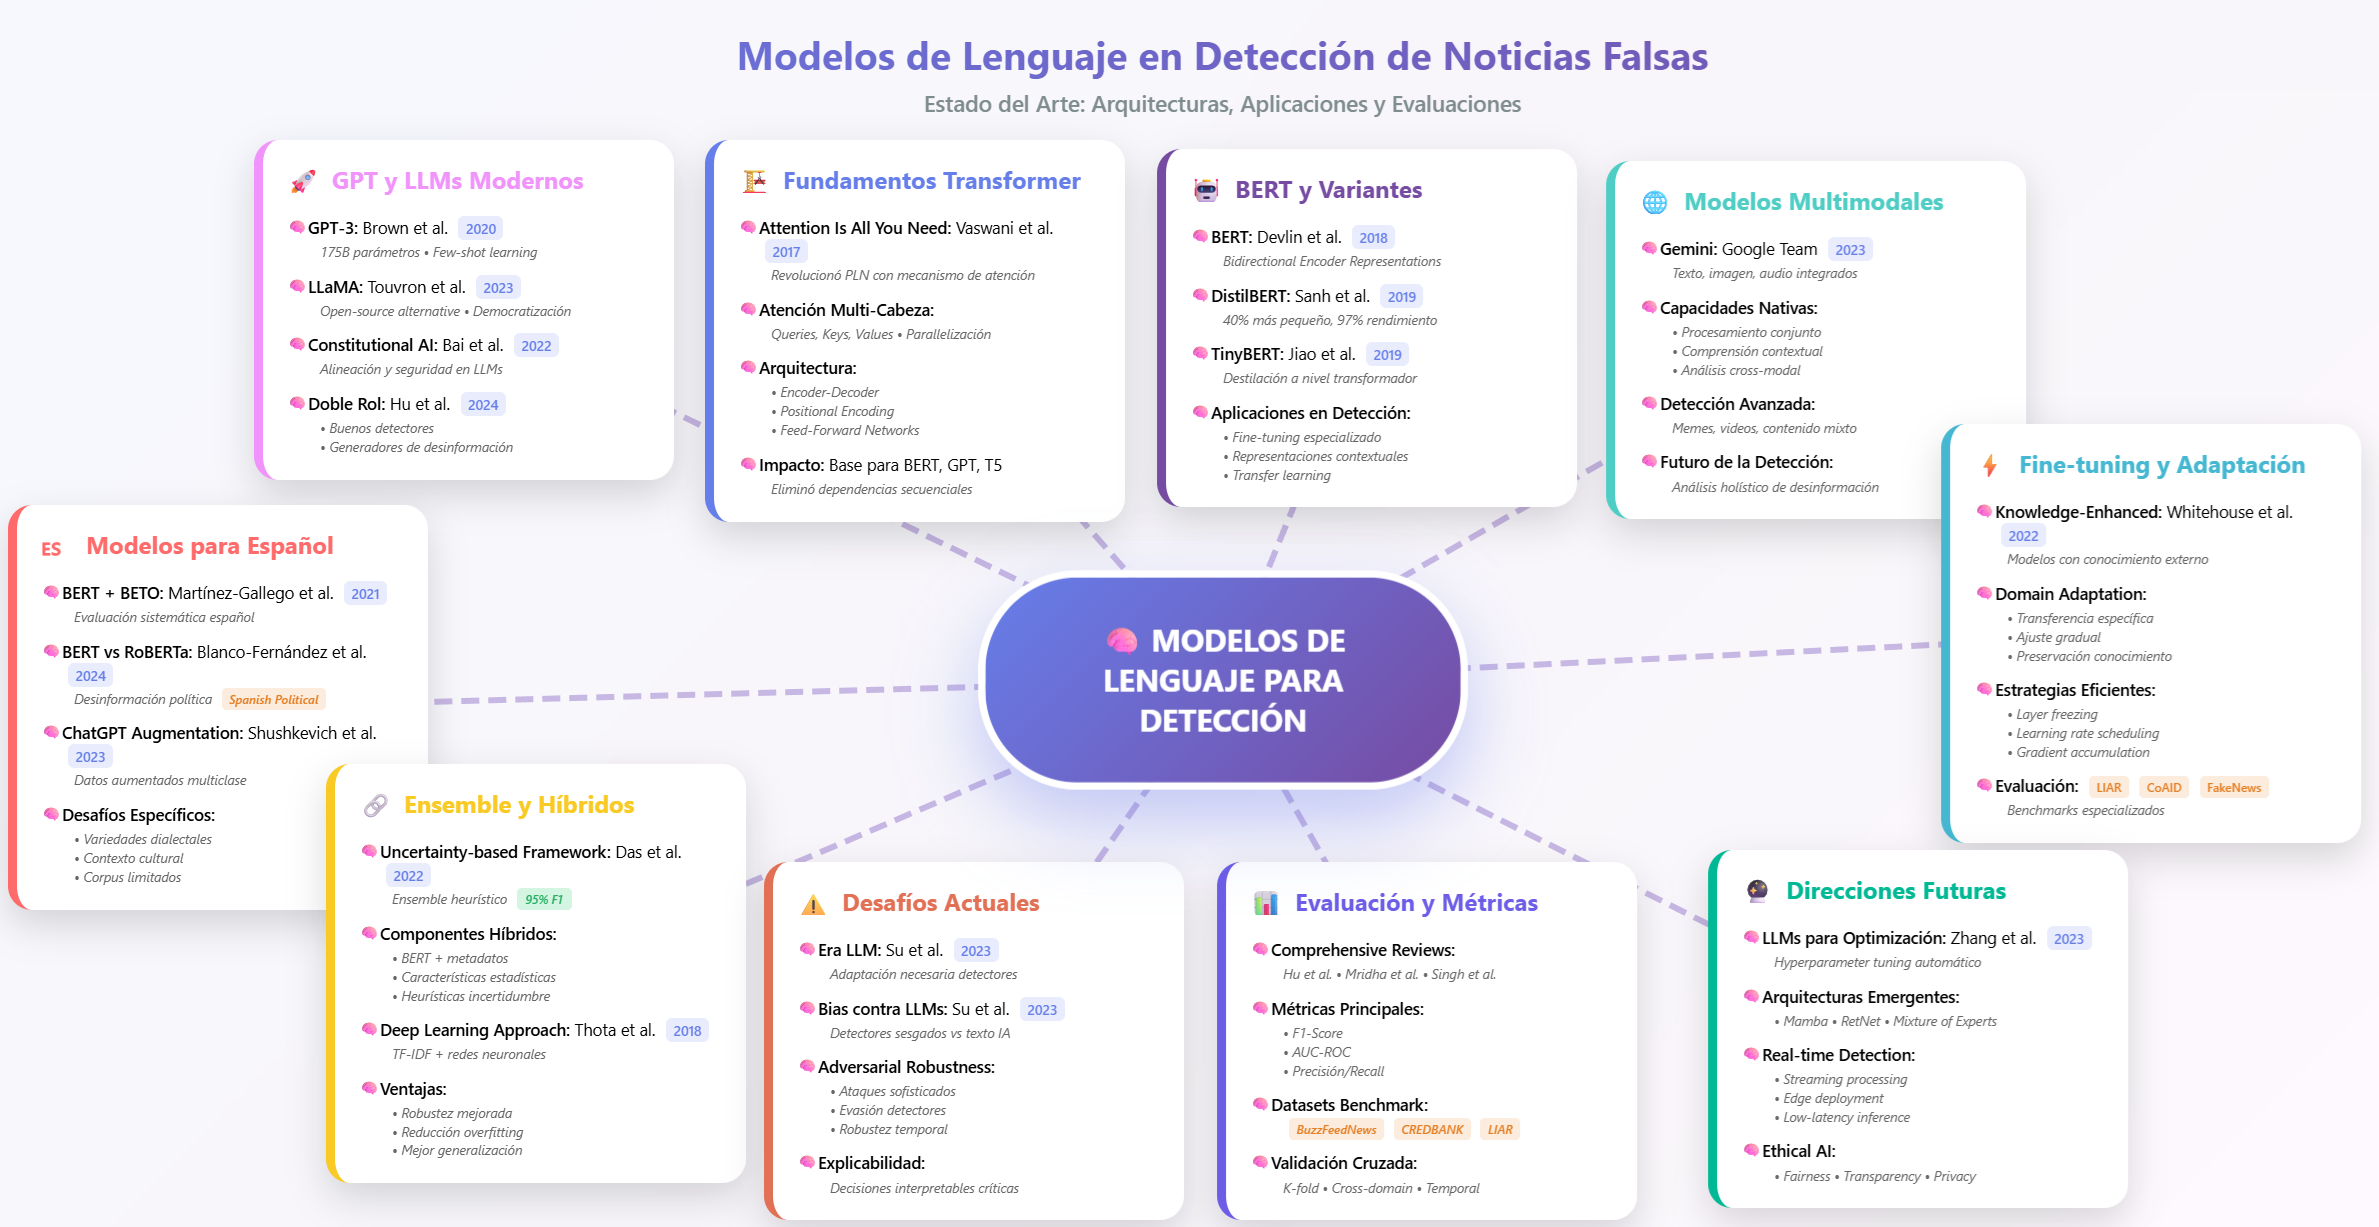
\includegraphics[width=\textwidth]{Imagenes/mapaConceptual3.png}
    \caption{Mapa Conceptual 3: Artículos que son revisiones o están relacionados al análisis de contenido y detección de fraude financiero.}
    \label{fig:mapa_conceptual_3}
\end{figure}

\begin{figure}[h!]
    \centering
    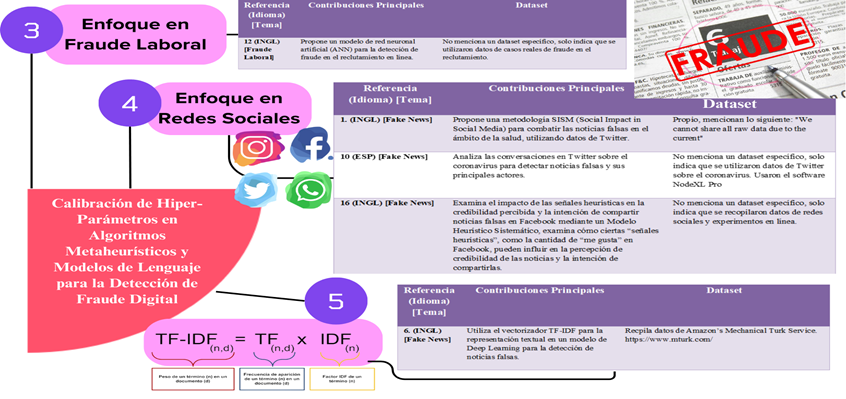
\includegraphics[width=\textwidth]{Imagenes/mapaConceptual4.png}
    \caption{Mapa Conceptual 4: Clasificación de artículos por enfoque metodológico.}
    \label{fig:mapa_conceptual_4}
\end{figure}

\begin{figure}[h!]
    \centering
    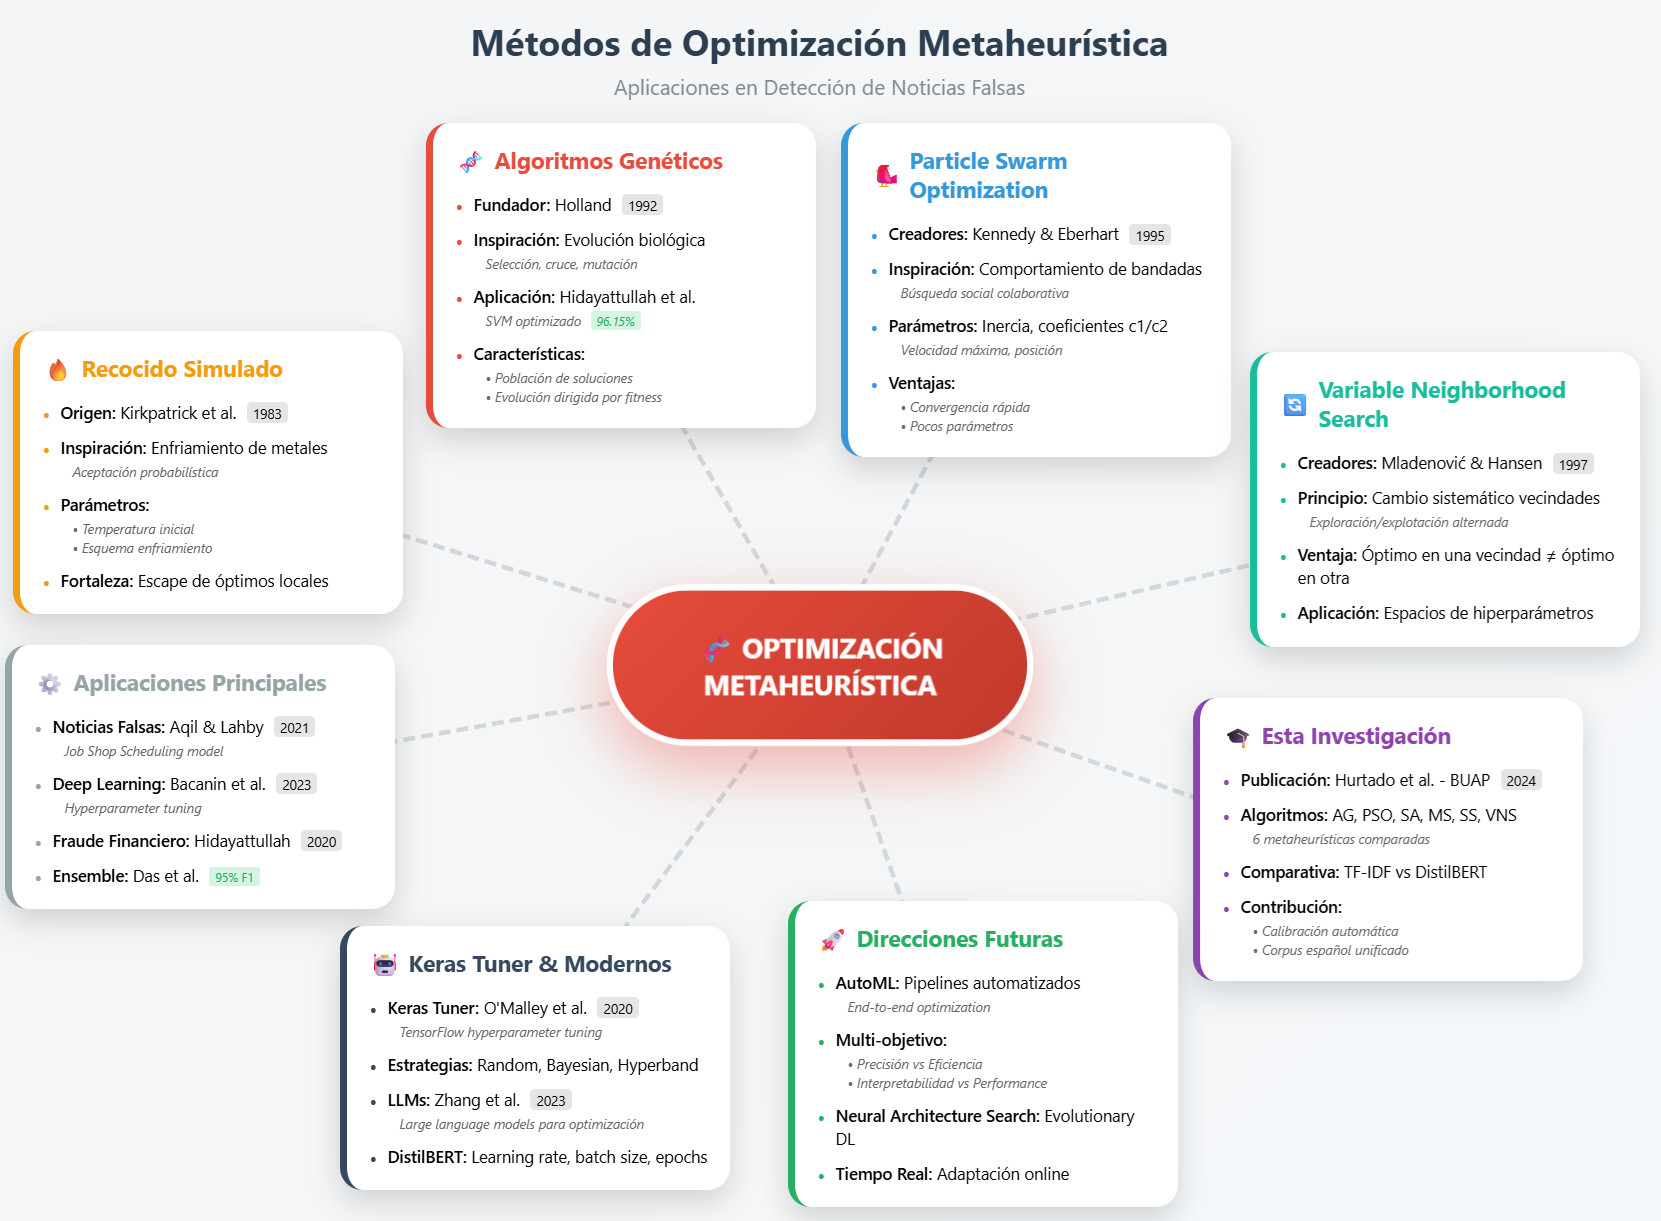
\includegraphics[width=\textwidth]{Imagenes/mapaConceptual5.png}
    \caption{Mapa Conceptual 5: Métodos de optimización y metaheurísticas aplicadas.}
    \label{fig:mapa_conceptual_5}
\end{figure}

\begin{figure}[h!]
    \centering
    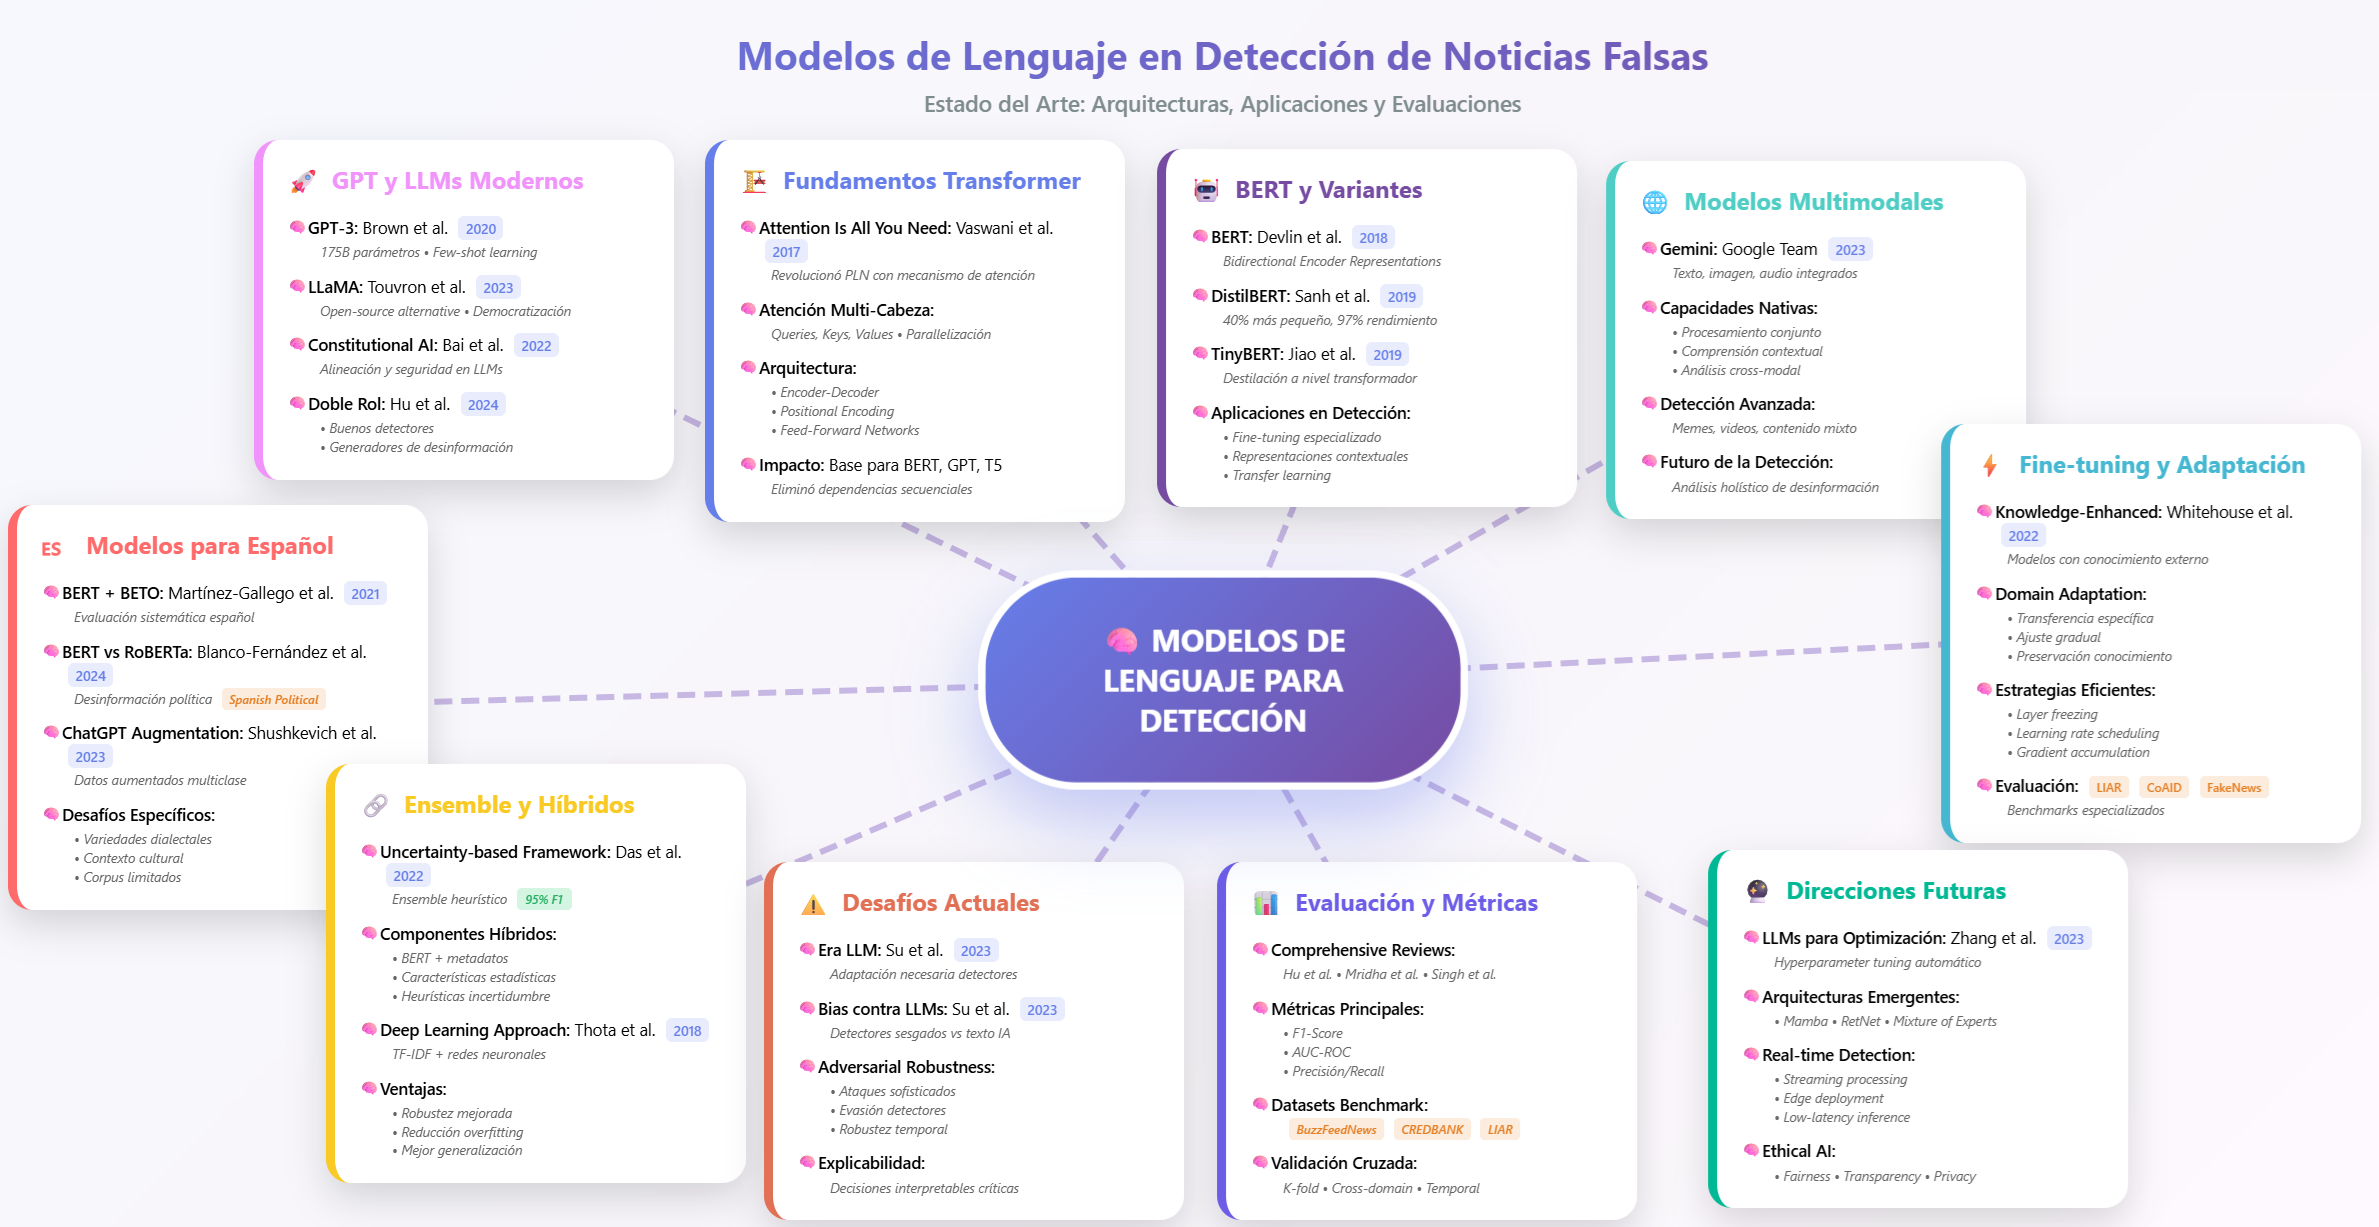
\includegraphics[width=\textwidth]{Imagenes/mapaConceptual6.png}
    \caption{Mapa Conceptual 6: Artículos relacionados que incorporan Modelos de Lenguaje.}
    \label{fig:mapa_conceptual_6}
\end{figure}

\section{Análisis Temático Comprehensivo de la Literatura Relevante}
\label{sec:analisis_tematico}

Más allá de la clasificación taxonómica superficial, resulta fundamental realizar un análisis en profundidad de las contribuciones clave de cada grupo temático identificado, examinando no solo qué se ha hecho, sino cómo se ha hecho, qué resultados se han obtenido, y cuáles son las implicaciones para la planeación y ejecución metodológica de esta tesis. Esta sección proporciona un análisis crítico y detallado de los aportes más significativos de cada categoría de investigación.

\subsection{El Desafío Fundamental de los Datos: Creación y Curación de Corpus en Español}

Uno de los desafíos más fundamentales y persistentes para el Procesamiento del Lenguaje Natural en español es la notable escasez de conjuntos de datos etiquetados de alta calidad a gran escala, especialmente en comparación con los abundantes recursos disponibles en inglés. Esta disparidad en recursos no es meramente cuantitativa, sino que refleja diferencias cualitativas en metodologías de construcción, criterios de calidad, y marcos de evaluación que han limitado históricamente el desarrollo de sistemas de PLN para español.

La creación y curación sistemática de corpus especializados constituye, por tanto, una línea de investigación fundamental que requiere no solo expertise técnico sino también comprensión profunda de las particularidades lingüísticas y culturales del español. El trabajo pionero de Fin de Maestría de Zules Acosta \cite{acosta2019construccion} fue uno de los pioneros más influyentes en este ámbito específico, centrándose meticulosamente en la creación de un conjunto de datos comprensivo de 598 noticias en castellano. Su investigación trasciende la mera recolección de datos para enfocarse profundamente en la importancia crítica de la \textit{ingeniería de características} para seleccionar estrategias óptimas de extracción que permitan a los modelos de aprendizaje automático clasificar eficazmente la veracidad del contenido. El trabajo incluye un análisis detallado de métricas de calidad, procedimientos de validación inter-anotador, y metodologías para manejar ambigüedad en el etiquetado de contenido borderline.

Por otro lado, el trabajo metodológicamente robusto de Posadas-Durán et al. \cite{posadas2019detection} introdujo el influyente \textit{Spanish Fake News Corpus} (con 971 noticias cuidadosamente seleccionadas), estableciéndose como un recurso fundamental para analizar y detectar información engañosa mediante métodos innovadores basados en el estilo de la escritura y características estilométricas avanzadas. Este corpus ha sido fundamental en competencias internacionales como IberLEF, donde se han evaluado sistemáticamente diversas metodologías para el español \cite{gomez2021overview}, incluyendo el análisis especializado de agresividad y noticias falsas en el español de México \cite{aragon2020overview}. La contribución incluye anotaciones de características lingüísticas profundas como complejidad sintáctica, diversidad léxica, y patrones discursivos específicos.

Más recientemente, se han publicado corpus de escala considerablemente mayor que han resultado cruciales para el avance del campo y específicamente para esta tesis. Tretiakov et al. \cite{tretiakov2022detection} aportaron un conjunto de datos significativamente expandido con 1,958 noticias falsas en español, incorporando metadatos enriquecidos sobre fuentes, fechas de publicación, y categorías temáticas. Paralelamente, el trabajo de gran escala de Blanco-Fernández et al. \cite{blanco2024enhancing} introdujo el ambicioso \textit{Spanish Political Fake News Dataset}. Este último recurso, con más de 57,000 noticias meticulosamente recolectadas y etiquetadas, representa uno de los mayores y más comprehensivos recursos disponibles para investigación en español y constituye la fuente principal de datos para esta tesis. La unificación metodológica de estos cuatro corpus diversos constituye el fundamento empírico sólido de este trabajo de investigación.

\subsection{Revolución de los Modelos de Lenguaje y Arquitecturas Transformer}

La arquitectura Transformer, introducida revolucionariamente por Vaswani et al. \cite{vaswani2017attention}, transformó completamente el panorama del PLN con su mecanismo de atención multi-cabeza innovador que permite el procesamiento paralelo eficiente y la captura de dependencias a largo plazo. Este trabajo fundamental estableció las bases teóricas y prácticas para una nueva generación de modelos como BERT \cite{devlin2018bert}, que introdujo el concepto paradigmático de pre-entrenamiento bidireccional, permitiendo a los modelos capturar contexto tanto precedente como subsecuente simultáneamente.

Las variantes optimizadas como DistilBERT \cite{sanh2019distilbert} y TinyBERT \cite{jiao2019tinybert} han demostrado que es posible mantener capacidades semánticas sofisticadas mientras se reduce dramáticamente el costo computacional, haciendo viable la implementación de sistemas de detección en dispositivos con recursos limitados y aplicaciones en tiempo real. Estas innovaciones en eficiencia son particularmente relevantes para implementaciones prácticas de sistemas de detección que deben operar bajo restricciones de latencia y recursos.

El paradigma de los Grandes Modelos de Lenguaje (LLMs) se consolidó definitivamente con GPT-3 \cite{brown2020language}, que demostró capacidades emergentes extraordinarias de few-shot learning y razonamiento en contexto que revolucionaron las expectativas sobre lo que los modelos de lenguaje pueden lograr. Trabajos más recientes como LLaMA \cite{touvron2023llama} han democratizado significativamente el acceso a modelos de gran escala mediante arquitecturas más eficientes y políticas de licenciamiento abierto, mientras que Gemini \cite{gemini2023family} ha avanzado hacia capacidades multimodales que integran texto, imágenes, y otros tipos de información. La investigación en IA Constitucional \cite{bai2022constitutional} ha abordado proactivamente los desafíos críticos de alineación y seguridad de estos sistemas poderosos.

Para el español específicamente, Martínez-Gallego et al. \cite{martinez2021fake} realizaron una exploración sistemática y comprehensiva de la aplicación de BERT y BETO, demostrando empíricamente las ventajas de modelos especializados lingüísticamente. Paralelamente, Blanco-Fernández et al. \cite{blanco2024enhancing} llevaron a cabo comparaciones detalladas entre BERT y RoBERTa para la detección de desinformación, proporcionando evidencia empírica sobre las ventajas específicas de diferentes arquitecturas transformer para este dominio.

La investigación sobre el rol dual de los LLMs \cite{hu2024bad, su2023adapting, su2023fake} ha revelado tanto oportunidades extraordinarias como desafíos significativos en su aplicación para la detección de noticias falsas, incluyendo cuestiones de sesgo, robustez, y generalización que requieren consideración cuidadosa en implementaciones prácticas.

\subsection{Optimización y Metaheurísticas en la Detección: Enfoques Innovadores}

Los algoritmos metaheurísticos han demostrado ser herramientas excepcionalmente valiosas para abordar problemas complejos de optimización en la detección de noticias falsas, proporcionando soluciones elegantes a desafíos que tradicionalmente han sido abordados mediante métodos menos sofisticados. Aqil y Lahby \cite{aqil2021modeling} desarrollaron una formulación innovadora que modela la detección como un problema de scheduling complejo, aplicando algoritmos genéticos, optimización por enjambre de partículas, y otras metaheurísticas para optimizar el pipeline completo de procesamiento.

La calibración de hiperparámetros \cite{bacanin2023benefits, hurtado2024calibracion} ha emergido como una aplicación crítica donde las metaheurísticas superan consistentemente a los métodos tradicionales de grid search y random search, especialmente en espacios de alta dimensionalidad donde la búsqueda exhaustiva es computacionalmente prohibitiva. Estos enfoques han demostrado capacidad superior para navegar paisajes de optimización complejos y multimodales característicos del ajuste de modelos profundos.

El enfoque innovador de ensemble con marcos heurísticos \cite{das2022heuristic} ha mostrado resultados especialmente prometedores al combinar múltiples modelos especializados con información estadística adicional, creando sistemas que pueden manejar incertidumbre de manera más sofisticada que enfoques de clasificación tradicionales. Yildirim \cite{yildirim2023novel} propuso un enfoque híbrido multi-thread particularmente avanzado que optimiza simultáneamente tanto la selección de características como los parámetros del modelo, demostrando el potencial de optimización coordinada en múltiples dimensiones del problema.

La aplicación de PSO para la detección de reseñas falsas \cite{deshai2023unmasking} demuestra convincentemente la versatilidad y transferabilidad de estas técnicas más allá del dominio específico de noticias, sugiriendo principios generalizables para la detección de contenido desinformativo en múltiples contextos.

\subsection{Aplicación de Metaheurísticas por Tipo de Detección}
\label{subsec:metaheuristicas_por_tipo}

La literatura revisada revela patrones específicos y sistemáticos en la aplicación de algoritmos metaheurísticos según el tipo de detección, el dominio del problema, y las características específicas de los datos involucrados. Esta taxonomía detallada proporciona insights valiosos para la selección informada de técnicas de optimización para diferentes contextos de aplicación.

\begin{table}[htbp]
\centering
\adjustbox{width=\textwidth,center}{%
\small
\begin{tabular}{|l|l|l|l|c|}
\hline
\rowcolor{UAMPurple!20}
\textbf{Tipo de Detección} & \textbf{Metaheurística Empleada} & \textbf{Aplicación Específica} & \textbf{Autores} & \textbf{Ref.} \\
\hline
\begin{tabular}[t]{@{}l@{}}Detección de\\Noticias Falsas\end{tabular} & \begin{tabular}[t]{@{}l@{}}Algoritmo Genético (GA),\\Colonia de Abejas (ABC),\\Búsqueda Iterativa (IG)\end{tabular} & \begin{tabular}[t]{@{}l@{}}Planificación de tareas\\para procesamiento\\de documentos\end{tabular} & Aqil, S. \& Lahby, M. & \cite{aqil2021modeling} \\
\hline
\begin{tabular}[t]{@{}l@{}}Detección de\\Reseñas Falsas\end{tabular} & \begin{tabular}[t]{@{}l@{}}Optimización por\\Enjambre de Partículas\\Adaptativo (PSO)\end{tabular} & \begin{tabular}[t]{@{}l@{}}Optimización de\\hiperparámetros en\\redes CNN\end{tabular} & \begin{tabular}[t]{@{}l@{}}Deshai, N. \&\\Rao, B. B.\end{tabular} & \cite{deshai2023unmasking} \\
\hline
\begin{tabular}[t]{@{}l@{}}Fraude Financiero\\y de Estados\\Financieros\end{tabular} & \begin{tabular}[t]{@{}l@{}}Algoritmos Genéticos,\\Optimización por\\Enjambre de Partículas,\\Recocido Simulado\end{tabular} & \begin{tabular}[t]{@{}l@{}}Selección de características\\y optimización de\\clasificadores SVM\end{tabular} & \begin{tabular}[t]{@{}l@{}}Hidayattullah, S.\\et al.\end{tabular} & \cite{hidayattullah2020financial} \\
\hline
\begin{tabular}[t]{@{}l@{}}Predicción de\\Dificultades\\Financieras\end{tabular} & \begin{tabular}[t]{@{}l@{}}Optimización Bayesiana\\con Procesos\\Gaussianos\end{tabular} & \begin{tabular}[t]{@{}l@{}}Calibración de\\hiperparámetros\\en modelos GPR\end{tabular} & \begin{tabular}[t]{@{}l@{}}Horak, J. \&\\Sabek, A.\end{tabular} & \cite{horak2023gaussian} \\
\hline
\begin{tabular}[t]{@{}l@{}}Detección de\\Fraude Laboral\end{tabular} & \begin{tabular}[t]{@{}l@{}}Redes Neuronales\\Artificiales (ANN)\end{tabular} & \begin{tabular}[t]{@{}l@{}}Clasificación de\\ofertas de empleo\\fraudulentas\end{tabular} & \begin{tabular}[t]{@{}l@{}}Nasser, I. M.\\et al.\end{tabular} & \cite{nasser2021online} \\
\hline
\begin{tabular}[t]{@{}l@{}}Optimización de\\Modelos de Energía\end{tabular} & \begin{tabular}[t]{@{}l@{}}Algoritmo Genético\\Binario, PSO, Recocido\\Simulado, Búsqueda\\Armónica\end{tabular} & \begin{tabular}[t]{@{}l@{}}Ajuste de hiperparámetros\\en modelos LSTM\\para predicción energética\end{tabular} & \begin{tabular}[t]{@{}l@{}}Bacanin, N.\\et al.\end{tabular} & \cite{bacanin2023benefits} \\
\hline
\begin{tabular}[t]{@{}l@{}}Detección Multimodal\\de Noticias Falsas\end{tabular} & \begin{tabular}[t]{@{}l@{}}Enfoque Híbrido\\Multi-hilo con\\Metaheurísticas\end{tabular} & \begin{tabular}[t]{@{}l@{}}Optimización paralela\\de características\\textuales y visuales\end{tabular} & Yildirim, G. & \cite{yildirim2023novel} \\
\hline
\begin{tabular}[t]{@{}l@{}}Selección de\\Características\\para Fake News\end{tabular} & \begin{tabular}[t]{@{}l@{}}K-Means combinado\\con Support Vector\\Machine (SVM)\end{tabular} & \begin{tabular}[t]{@{}l@{}}Reducción de\\dimensionalidad\\y mejora de precisión\end{tabular} & \begin{tabular}[t]{@{}l@{}}Yazdi, K. M.\\et al.\end{tabular} & \cite{yazdi2020improving} \\
\hline
\begin{tabular}[t]{@{}l@{}}Framework de\\Incertidumbre\\para Fake News\end{tabular} & \begin{tabular}[t]{@{}l@{}}Enfoque Heurístico\\basado en Ensemble\end{tabular} & \begin{tabular}[t]{@{}l@{}}Manejo de incertidumbre\\en clasificación de\\tweets y artículos\end{tabular} & \begin{tabular}[t]{@{}l@{}}Das, S. D.\\et al.\end{tabular} & \cite{das2022heuristic} \\
\hline
\begin{tabular}[t]{@{}l@{}}Optimización de\\Dominación Total\\en Redes Sociales\end{tabular} & \begin{tabular}[t]{@{}l@{}}Búsqueda en\\Vecindades Variables\\(VNS)\end{tabular} & \begin{tabular}[t]{@{}l@{}}Propagación de\\información en\\redes sociales\end{tabular} & \begin{tabular}[t]{@{}l@{}}Kapunac, S.\\et al.\end{tabular} & \cite{kapunac2023variable} \\
\hline
\begin{tabular}[t]{@{}l@{}}Estimación de\\Esfuerzo en\\Proyectos\end{tabular} & \begin{tabular}[t]{@{}l@{}}Ensemble con\\Metaheurísticas\\para Pesos\end{tabular} & \begin{tabular}[t]{@{}l@{}}Optimización de\\hiperparámetros\\y pesos de ensemble\end{tabular} & \begin{tabular}[t]{@{}l@{}}Yasmin, A.\\et al.\end{tabular} & \cite{yasmin2024ensemble} \\
\hline
\end{tabular}
}
\caption{Aplicación de metaheurísticas por tipo de detección en la literatura revisada.}
\label{tab:metaheuristicas_deteccion}
\end{table}

\subsubsection{Patrones Identificados por Dominio}

Del análisis sistemático de la literatura se identifican tres patrones principales y claramente diferenciados en la aplicación de metaheurísticas:

\paragraph{Detección de Contenido Textual}
Para la detección de noticias falsas y contenido textual fraudulento, predominan los enfoques que combinan estratégicamente:
\begin{itemize}
    \item \textbf{Algoritmos Genéticos}: Utilizados principalmente para selección de características en espacios de alta dimensionalidad y optimización de arquitecturas de modelos complejos \cite{aqil2021modeling, hidayattullah2020financial}
    \item \textbf{PSO Adaptativo}: Especialmente efectivo para la calibración de hiperparámetros en redes neuronales complejas donde el espacio de búsqueda es continuo y las evaluaciones son costosas \cite{deshai2023unmasking, bacanin2023benefits}
    \item \textbf{Enfoques Híbridos}: Combinación sinérgica de múltiples metaheurísticas para diferentes aspectos del pipeline de detección, optimizando simultáneamente múltiples objetivos \cite{yildirim2023novel}
\end{itemize}

\paragraph{Optimización de Modelos de Aprendizaje Profundo}
En aplicaciones que involucran modelos de aprendizaje profundo y arquitecturas complejas, se observa una preferencia marcada por:
\begin{itemize}
    \item \textbf{Recocido Simulado}: Particularmente efectivo para escapar de óptimos locales en espacios de hiperparámetros complejos y multimodales \cite{bacanin2023benefits}
    \item \textbf{Optimización Bayesiana}: Para calibración eficiente en modelos probabilísticos donde se requiere balance entre exploración y explotación \cite{horak2023gaussian}
    \item \textbf{Búsqueda en Vecindades Variables}: Para exploración sistemática de configuraciones de red mediante cambio de estructuras de vecindad \cite{kapunac2023variable}
\end{itemize}

\paragraph{Sistemas de Detección en Tiempo Real}
Para aplicaciones que requieren procesamiento en tiempo real y alta throughput, las metaheurísticas se enfocan estratégicamente en:
\begin{itemize}
    \item \textbf{Algoritmos de Planificación}: Como IG (Iterated Greedy) para optimización de tareas de procesamiento con restricciones temporales \cite{aqil2021modeling}
    \item \textbf{Métodos Ensemble}: Con optimización de pesos mediante metaheurísticas para combinar múltiples detectores especializados \cite{das2022heuristic, yasmin2024ensemble}
    \item \textbf{Enfoques Multi-hilo}: Para paralelización eficiente de la optimización en sistemas multimodales que procesan múltiples tipos de información simultáneamente \cite{yildirim2023novel}
\end{itemize}

Esta taxonomía detallada revela que la elección de la metaheurística está fuertemente influenciada por factores como el tipo de modelo subyacente, las características del conjunto de datos, los requisitos de rendimiento temporal del sistema de detección, y las restricciones computacionales específicas del entorno de implementación.

\subsection{Perspectivas Interdisciplinarias y Análisis Social}

La comprensión profunda del fenómeno de las noticias falsas requiere necesariamente un enfoque interdisciplinario sofisticado que combine aspectos técnicos avanzados con análisis social, psicológico, y cultural. Los aspectos puramente técnicos, aunque fundamentales, son insuficientes para abordar completamente la complejidad multifacética de la desinformación moderna.

Ali et al. \cite{ali2021fake, ali2020posttruth} han investigado sistemáticamente cómo las heurísticas cognitivas humanas, incluyendo señales de popularidad social como el número de ``me gusta'' y compartidos, influyen significativamente en la percepción de credibilidad de contenido digital. Su trabajo sobre el procesamiento heurístico durante eventos políticos específicos, particularmente las elecciones presidenciales de 2016 en Estados Unidos, proporciona insights valiosos y empíricamente fundamentados sobre la psicología de la desinformación y los mecanismos cognitivos que hacen a las personas susceptibles a información falsa.

El análisis detallado del rol de los medios de comunicación tradicionales \cite{carcamo2021fake, perez2020fake} ha revelado patrones culturales importantes en cómo diferentes países y culturas abordan, conceptualizan, y responden al problema de la desinformación. Estos estudios transculturales proporcionan evidencia empírica sobre la importancia de considerar factores culturales en el diseño de sistemas de detección automatizada.

Pulido et al. \cite{pulido2020new} propusieron el marco innovador SISM (Social Impact in Social Media) para combatir específicamente la desinformación en el dominio de la salud, un área particularmente crítica durante pandemias y crisis de salud pública donde la desinformación puede tener consecuencias directas sobre la vida y muerte de las personas.

\subsection{Detección de Fraude: Extensión Más Allá de las Noticias}

La investigación en detección de fraude ha diversificado significativamente sus aplicaciones, extendiéndose más allá del dominio específico de noticias falsas hacia otros contextos de fraude digital que presentan características similares pero requieren adaptaciones específicas.

En el ámbito laboral específicamente, Nasser et al. \cite{nasser2021online} desarrollaron sistemas basados en redes neuronales artificiales para detectar ofertas de trabajo fraudulentas, demostrando que las técnicas desarrolladas para detección de noticias falsas pueden transferirse efectivamente a otros dominios textuales. Paralelamente, Alvarez \cite{alvarez2021fraude} analizó comprehensivamente las nuevas modalidades de fraude laboral en la era digital latinoamericana, proporcionando contexto regional importante para entender las manifestaciones específicas del fraude en diferentes contextos socioeconómicos.

En el sector financiero, la investigación de Hidayattullah et al. \cite{hidayattullah2020financial} demostró empíricamente la efectividad de combinar aprendizaje automático con optimización metaheurística para detectar fraudes en estados financieros, estableciendo precedentes metodológicos importantes. Cao et al. \cite{cao2020corporate} establecieron conexiones innovadoras entre indicadores de empleo corporativo y riesgo de fraude, proporcionando herramientas valiosas para auditores y reguladores financieros.

\section{Síntesis y Perspectivas Futuras}
\label{sec:sintesis_perspectivas}

La revisión comprehensiva y sistemática de la literatura revela una evolución clara y acelerada en las aproximaciones para la detección de noticias falsas y fraude digital. Desde los primeros enfoques relativamente simples basados en características lingüísticas superficiales hasta los modernos sistemas sofisticados basados en transformers y LLMs, el campo ha experimentado avances extraordinarios en términos de precisión, escalabilidad, y aplicabilidad práctica.

Los desafíos principales identificados a través de esta revisión incluyen: (1) la necesidad imperativa de mayor cantidad de datos etiquetados de alta calidad en español, (2) la adaptación cultural y lingüística de modelos a contextos específicos del mundo hispanohablante, (3) la optimización eficiente de hiperparámetros en modelos cada vez más complejos, y (4) la integración inteligente de información multimodal y conocimiento externo estructurado.

Esta tesis contribuye especialmente a los puntos (1) y (3) mediante la unificación metodológica de corpus existentes en una escala sin precedentes y la aplicación sistemática de técnicas metaheurísticas avanzadas para la optimización de modelos de detección de última generación.

La organización temática comprehensiva presentada en este capítulo proporciona un marco conceptual robusto para entender las diferentes dimensiones del problema de detección de desinformación y justifica empíricamente la aproximación metodológica híbrida adoptada en esta investigación, que combina inteligentemente modelos de lenguaje state-of-the-art con técnicas de optimización metaheurística para lograr rendimiento superior en la detección de contenido desinformativo en español.

Las perspectivas futuras incluyen la evolución hacia sistemas adaptativos que puedan evolucionar con las técnicas de desinformación cambiantes, la integración de conocimiento factual en tiempo real, y el desarrollo de marcos éticos para el despliegue responsable de tecnologías de detección automatizada.
%!TEX root = ../ICR.tex
\chapter{Metodología \label{cap:Metodologia}}

En este capítulo se detalla el procedimiento experimental seguido para abordar el problema de la detección de noticias falsas en español. La metodología se diseñó con un enfoque evolutivo y comparativo, comenzando con una exploración de técnicas de optimización clásicas y culminando con la implementación de un modelo de lenguaje de última generación. El diseño del flujo de trabajo, ilustrado en la Figura \ref{fig:metodologia_general}, garantiza la reproducibilidad de los resultados al definir claramente cada una de sus etapas, desde la recopilación de datos hasta la evaluación final y la implementación de una aplicación web como solución práctica.

\section{Visión General de la Metodología}

La estrategia metodológica de esta tesis se fundamenta en la comparación sistemática de dos paradigmas de la inteligencia artificial sobre un corpus unificado de gran escala. Como se muestra en la Figura \ref{fig:metodologia_general}, ambos enfoques parten de una base común (la problemática y los datos), pero siguen rutas de implementación y modelado distintas, para finalmente ser evaluados bajo un mismo marco de métricas y así determinar la solución más eficaz que será implementada en una aplicación web.

El primer paradigma se basa en técnicas clásicas de Procesamiento del Lenguaje Natural (PLN) con representación Bolsa de Palabras (BoW) y optimización metaheurística, mientras que el segundo emplea modelos Transformer pre-entrenados con técnicas de fine-tuning. Esta aproximación comparativa permite evaluar tanto la efectividad como la eficiencia computacional de cada enfoque en el contexto específico de la detección de desinformación en español.

Una vez determinado el mejor modelo mediante las métricas de evaluación correspondientes, se procederá a desarrollar una aplicación web funcional que permita la detección automática de noticias falsas en tiempo real.

\begin{figure}[h!]
    \centering
    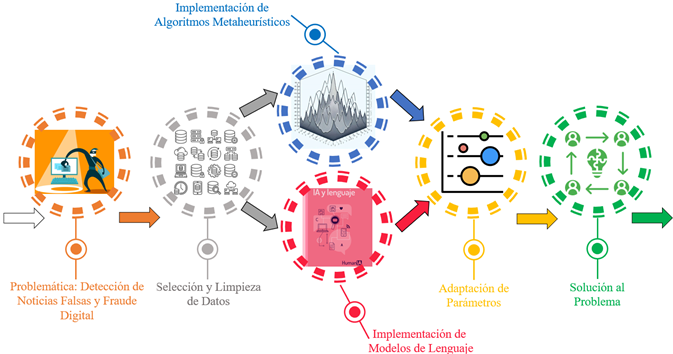
\includegraphics[width=\textwidth]{Imagenes/metodologiaCompleta.png}
    \caption{Metodología propuesta que aborda la problemática combinando Algoritmos Metaheurísticos y Modelos de Lenguaje.}
    \label{fig:metodologia_general}
\end{figure}

\section{Definición y Distinción de Conceptos Fundamentales}
\label{sec:definicion_conceptos}

Antes de proceder con la descripción metodológica, es fundamental establecer con precisión la terminología utilizada en esta investigación, particularmente la distinción entre conceptos relacionados pero diferenciados que a menudo se utilizan de manera intercambiable en la literatura.

\subsection{Noticia Falsa vs. Bulo: Una Distinción Crítica}

En el contexto de esta investigación, es esencial distinguir entre dos conceptos fundamentales que, aunque relacionados, poseen características distintivas importantes para el desarrollo de sistemas de detección automática.

% Definir colores adicionales para las tablas de conceptos
\definecolor{LightGreen}{RGB}{144, 238, 144}
\definecolor{LightCoral}{RGB}{240, 128, 128}
\definecolor{LightSkyBlue}{RGB}{135, 206, 250}
\definecolor{LightGoldenrod}{RGB}{250, 250, 210}
\definecolor{LightPink}{RGB}{255, 182, 193}

\begin{table}[htbp]
\centering
\adjustbox{width=\textwidth,center}{%
\footnotesize
\begin{tabular}{|l|p{6cm}|p{6cm}|}
\hline
\rowcolor{UAMPurple!20}
\textbf{Aspecto} & \textbf{Noticia Falsa} & \textbf{Bulo} \\
\hline
\rowcolor{LightGreen!30}
\textbf{Definición} & 
\begin{tabular}[t]{@{}l@{}}Información deliberadamente fabricada\\que se presenta como noticia legítima,\\pero contiene datos falsos, inexactos\\o engañosos\end{tabular} & 
\begin{tabular}[t]{@{}l@{}}Información falsa que circula\\ampliamente, especialmente en redes\\sociales, con propósito de engañar\\a la audiencia\end{tabular} \\
\hline
\rowcolor{LightSkyBlue!30}
\textbf{Formato} & 
\begin{tabular}[t]{@{}l@{}}Apariencia de contenido periodístico\\real, formato de noticia tradicional\\con titular, cuerpo, fecha, fuente\end{tabular} & 
\begin{tabular}[t]{@{}l@{}}No necesariamente formato\\periodístico, puede ser texto libre,\\memes, cadenas de WhatsApp\end{tabular} \\
\hline
\rowcolor{LightCoral!30}
\textbf{Intención} & 
\begin{tabular}[t]{@{}l@{}}Intención maliciosa de desinformar\\simulando legitimidad periodística\end{tabular} & 
\begin{tabular}[t]{@{}l@{}}Propósito de engañar que apela\\más a emociones que a hechos\\verificables\end{tabular} \\
\hline
\rowcolor{LightGoldenrod!30}
\textbf{Propagación} & 
\begin{tabular}[t]{@{}l@{}}Se distribuye a través de sitios\\web que simulan medios legítimos\\o plataformas de noticias\end{tabular} & 
\begin{tabular}[t]{@{}l@{}}Circulación viral en redes sociales,\\aplicaciones de mensajería,\\cadenas de reenvío\end{tabular} \\
\hline
\rowcolor{LightPink!30}
\textbf{Ejemplos} & 
\begin{tabular}[t]{@{}l@{}}Artículos con titular sensacionalista,\\byline falso, citas inventadas,\\estadísticas manipuladas\end{tabular} & 
\begin{tabular}[t]{@{}l@{}}Teorías conspirativas, información\\médica falsa, rumores políticos,\\cadenas de "urgente"\end{tabular} \\
\hline
\rowcolor{HeaderBlue!20}
\textbf{Relevancia para PLN} & 
\begin{tabular}[t]{@{}l@{}}Estructura textual más predecible,\\patrones estilísticos identificables\\en el análisis automatizado\end{tabular} & 
\begin{tabular}[t]{@{}l@{}}Variabilidad estructural mayor,\\requiere análisis semántico\\y contextual más sofisticado\end{tabular} \\
\hline
\end{tabular}
}
\caption{Comparación detallada entre noticia falsa y bulo en el contexto de detección automática.}
\label{tab:noticia_falsa_vs_bulo}
\end{table}

\subsection{Taxonomía de la Desinformación}

Para proporcionar un marco conceptual completo, esta investigación adopta la taxonomía establecida por la literatura internacional \cite{bondielli2019survey, hu2022deep}, que clasifica el contenido engañoso en tres categorías principales:

\begin{enumerate}
    \item \textbf{\gls{desinformacion}}: Información falsa creada y compartida deliberadamente con intención maliciosa
    \item \textbf{\gls{misinformacion}}: Información incorrecta compartida sin intención maliciosa
    \item \textbf{\gls{malinformacion}}: Información genuina compartida con intención de causar daño
\end{enumerate}

El alcance de esta investigación se centra específicamente en la detección automática de \textbf{desinformación}, abarcando tanto noticias falsas como bulos, reconociendo que ambos tipos requieren estrategias de procesamiento de lenguaje natural diferenciadas pero complementarias.

\subsection{Justificación de la Unificación Terminológica}

En el contexto del desarrollo de sistemas automáticos de detección, la distinción entre noticia falsa y bulo, aunque conceptualmente importante, se aborda mediante un enfoque unificado de \textbf{detección de contenido desinformativo}. Esta decisión metodológica se fundamenta en:

\begin{itemize}
    \item \textbf{Características textuales compartidas}: Ambos tipos utilizan patrones lingüísticos identificables mediante técnicas de PLN
    \item \textbf{Objetivo común}: La finalidad de engañar o desinformar a la audiencia
    \item \textbf{Impacto social similar}: Efectos negativos en la percepción pública y toma de decisiones
    \item \textbf{Necesidad práctica}: Los sistemas de detección automática deben ser capaces de identificar ambos tipos
\end{itemize}

Por tanto, en el resto de este documento, el término \textbf{``noticias falsas''} se utilizará de manera inclusiva para referirse a cualquier tipo de contenido desinformativo, reconociendo la diversidad de formatos y estrategias de propagación que abarca esta categorización.

\section{Construcción del Corpus Unificado}
\label{sec:construccion_corpus}

El primer y más fundamental paso de la metodología fue la construcción de un corpus de alta calidad y de tamaño significativo en español, dada la escasez documentada de recursos centralizados para esta tarea \cite{hu2022deep}.

% Definir colores adicionales para hacer las tablas más coloridas
\definecolor{LightGreen}{RGB}{144, 238, 144}
\definecolor{LightCoral}{RGB}{240, 128, 128}
\definecolor{LightSkyBlue}{RGB}{135, 206, 250}
\definecolor{LightGoldenrod}{RGB}{250, 250, 210}
\definecolor{LightPink}{RGB}{255, 182, 193}

\subsection{Fuentes de Datos Académicas}

Se llevó a cabo un proceso exhaustivo de investigación y unificación de cuatro corpus académicos reconocidos, los cuales constituyen pilares en la investigación de noticias falsas en español. La Tabla \ref{tab:corpus_academicos} presenta un resumen detallado de estos recursos.

\begin{table}[htbp]
\centering
\adjustbox{width=\textwidth,center}{%
\footnotesize
\begin{tabular}{|c|l|l|c|c|l|c|}
\hline
\rowcolor{UAMPurple!20}
\textbf{ID} & \textbf{Nombre del Corpus} & \textbf{Autores Principales} & \textbf{Año} & \textbf{Noticias} & \textbf{Características} & \textbf{Ref.} \\
\hline
\rowcolor{LightGreen!30}
1 & \begin{tabular}[t]{@{}l@{}}Spanish Fake News Corpus\\(IberLEF)\end{tabular} & \begin{tabular}[t]{@{}l@{}}Posadas-Durán, J.P.\\Gómez-Adorno, H.\end{tabular} & 2019-2021 & 971 & \begin{tabular}[t]{@{}l@{}}Análisis estilométrico\\Múltiples versiones\end{tabular} & \cite{posadas2019detection} \\
\hline
\rowcolor{LightSkyBlue!30}
2 & \begin{tabular}[t]{@{}l@{}}Dataset Zules Acosta\\(UPM)\end{tabular} & Acosta, F.A.Z. & 2019 & 598 & \begin{tabular}[t]{@{}l@{}}Trabajo fin de máster\\Web scraping verificado\end{tabular} & \cite{acosta2019construccion} \\
\hline
\rowcolor{LightCoral!30}
3 & \begin{tabular}[t]{@{}l@{}}Dataset Tretiakov\\(Kaggle)\end{tabular} & \begin{tabular}[t]{@{}l@{}}Tretiakov, A.\\Martín García, A.\end{tabular} & 2022 & 1,958 & \begin{tabular}[t]{@{}l@{}}Machine Learning\\Disponible públicamente\end{tabular} & \cite{tretiakov2022detection} \\
\hline
\rowcolor{LightGoldenrod!30}
4 & \begin{tabular}[t]{@{}l@{}}Spanish Political Fake News\\Dataset\end{tabular} & \begin{tabular}[t]{@{}l@{}}Blanco-Fernández, Y.\\Otero-Vizoso, J.\end{tabular} & 2024 & 57,231 & \begin{tabular}[t]{@{}l@{}}Temática política\\Modelos BERT/RoBERTa\end{tabular} & \cite{blanco2024enhancing} \\
\hline
\rowcolor{HeaderBlue!20}
\multicolumn{5}{|c|}{\textbf{TOTAL CORPUS ACADÉMICOS}} & \textbf{60,758} & \textbf{Cuatro fuentes} \\
\hline
\end{tabular}
}
\caption{Corpus académicos utilizados para la construcción del dataset unificado.}
\label{tab:corpus_academicos}
\end{table}

\subsubsection{Spanish Fake News Corpus (IberLEF)}

Este corpus, asociado a las competencias de IberLEF y desarrollado por Posadas-Durán, Gómez-Adorno, et al., ha tenido varias versiones. La versión original y más citada del corpus contiene un total de 971 noticias \cite{posadas2019detection}. Este corpus se caracteriza por su enfoque en análisis estilométrico y ha sido utilizado en múltiples evaluaciones comparativas dentro del marco de las competencias IberLEF \cite{gomez2021overview, aragon2020overview}. Las versiones posteriores del corpus han sido mantenidas y actualizadas en repositorios públicos \cite{ramirez2021spanish}.

\subsubsection{Dataset de Zules Acosta (Universidad Politécnica de Madrid)}

Desarrollado como parte de un Trabajo Fin de Máster Universitario en Ciberseguridad en la Universidad Politécnica de Madrid, este corpus contiene 598 noticias verificadas \cite{acosta2019construccion}. El dataset fue construido mediante técnicas de web scraping y se encuentra disponible públicamente en la plataforma Kaggle \cite{acosta2019dataset, zules2019spanish}. Su contribución principal radica en la aplicación de metodologías rigurosas de verificación para la construcción de datasets de noticias falsas.

\subsubsection{Dataset de Tretiakov et al.}

Este corpus, desarrollado por Tretiakov, Martín García y Camacho, contiene 1,958 noticias falsas en español \cite{tretiakov2022detection}. El dataset fue creado en el contexto de técnicas de aprendizaje automático para la detección de información falsa y se encuentra disponible públicamente en Kaggle \cite{tretiakov2022noticias}. Su enfoque se centra en la aplicación de técnicas de machine learning para la clasificación automatizada de contenido desinformativo.

\subsubsection{Spanish Political Fake News Dataset}

El corpus más extenso utilizado, desarrollado por Blanco-Fernández et al., contiene 57,231 noticias de temática política \cite{blanco2024enhancing}. Este dataset fue específicamente diseñado para evaluar modelos BERT y RoBERTa en la detección de desinformación política en español y se encuentra disponible en Kaggle \cite{blanco2024spanish}. Su gran tamaño y enfoque en contenido político lo convierte en un recurso valioso para el entrenamiento de modelos de gran escala.

\subsection{Proceso de Unificación y Estandarización}

La integración de corpus heterogéneos requirió un proceso sistemático de estandarización que incluyó:

\begin{enumerate}
    \item \textbf{Normalización de formato:} Unificación de esquemas de etiquetado en un sistema binario consistente (FALSO=0, REAL=1) y estandarización de estructuras de datos CSV con separador de punto y coma
    \item \textbf{Eliminación de duplicados:} Implementación de algoritmos de detección de contenido similar basados en hash de texto y comparación de títulos
    \item \textbf{Validación de calidad:} Verificación manual de una muestra estadísticamente significativa para confirmar la calidad del etiquetado y consistencia temática
    \item \textbf{Balanceado de clases:} Análisis detallado de la distribución de clases para identificar necesidades de ampliación y garantizar equilibrio
    \item \textbf{Limpieza de datos:} Eliminación de registros con valores nulos o inconsistentes mediante \texttt{dropna()} y validación de tipos de datos
\end{enumerate}

\subsection{Ampliación del Corpus Mediante Web Scraping}

Para mejorar el balance del conjunto de datos y aumentar la diversidad de las noticias etiquetadas como "FALSAS", se aplicaron técnicas de web scraping automatizado. Se desarrolló un script especializado en Python utilizando las librerías BeautifulSoup y Requests para extraer de forma sistemática los titulares y cuerpos de noticia del portal de contenido satírico "El Deforma".

\subsubsection{Proceso de Web Scraping Automatizado}

El proceso de extracción automatizada se ejecutó en múltiples fases para alcanzar el objetivo de 9,000 noticias adicionales. La Tabla \ref{tab:web_scraping_proceso} detalla las diferentes etapas implementadas.

\begin{table}[htbp]
\centering
\adjustbox{width=\textwidth,center}{%
\small
\begin{tabular}{|c|l|l|c|c|l|}
\hline
\rowcolor{UAMPurple!20}
\textbf{Fase} & \textbf{Estrategia} & \textbf{Técnica Utilizada} & \textbf{Objetivo} & \textbf{Resultado} & \textbf{Observaciones} \\
\hline
\rowcolor{LightGreen!30}
1 & Scraping Inicial & \begin{tabular}[t]{@{}l@{}}Navegación por enlaces\\Extracción de contenido\end{tabular} & 1,000 & 1,000 & \begin{tabular}[t]{@{}l@{}}Proceso exitoso\\Base establecida\end{tabular} \\
\hline
\rowcolor{LightSkyBlue!30}
2 & \begin{tabular}[t]{@{}l@{}}Búsqueda Expandida\\Masiva\end{tabular} & \begin{tabular}[t]{@{}l@{}}URLs desde existentes\\Crawling híbrido\end{tabular} & 9,000 & 2,495 & \begin{tabular}[t]{@{}l@{}}Expansión limitada\\Nuevas estrategias\end{tabular} \\
\hline
\rowcolor{LightCoral!30}
3 & \begin{tabular}[t]{@{}l@{}}Crawler Híbrido\\Persistente\end{tabular} & \begin{tabular}[t]{@{}l@{}}URLs semilla\\Trafilatura\end{tabular} & 9,000 & 2,495 & \begin{tabular}[t]{@{}l@{}}Estabilización\\Mismo resultado\end{tabular} \\
\hline
\rowcolor{LightGoldenrod!30}
4 & \begin{tabular}[t]{@{}l@{}}Paginación\\Sistemática\end{tabular} & \begin{tabular}[t]{@{}l@{}}Escaneo por páginas\\Indexación completa\end{tabular} & 9,000 & 9,000 & \begin{tabular}[t]{@{}l@{}}Éxito completo\\Objetivo alcanzado\end{tabular} \\
\hline
\rowcolor{HeaderBlue!20}
\multicolumn{4}{|c|}{\textbf{TOTAL EXTRAÍDO}} & \textbf{9,000} & \textbf{Web scraping completado} \\
\hline
\end{tabular}
}
\caption{Fases del proceso de web scraping implementado para "El Deforma".}
\label{tab:web_scraping_proceso}
\end{table}

\subsubsection{Implementación Técnica del Web Scraping}

El proceso de extracción automatizada incluyó:

\begin{enumerate}
    \item \textbf{Identificación de patrones:} Análisis de la estructura HTML del sitio web objetivo para identificar selectores CSS consistentes (\texttt{h1.tdb-title-text}, \texttt{div.tdb-block-inner})
    \item \textbf{Extracción automatizada:} Implementación de rutinas de scraping con manejo de errores y delays aleatorios (1.5-4.5 segundos) para evitar sobrecarga del servidor
    \item \textbf{Validación de contenido:} Verificación automática de la calidad del contenido extraído mediante filtros de longitud mínima (500 caracteres)
    \item \textbf{Limpieza de texto:} Eliminación de disclaimers específicos del sitio, caracteres especiales y normalización de espacios mediante expresiones regulares
    \item \textbf{Etiquetado automático:} Asignación de etiqueta "FALSO" (0) a todo el contenido extraído del portal satírico
    \item \textbf{Persistencia progresiva:} Guardado en lotes de 50 registros con formato CSV y separador de punto y coma para evitar pérdida de datos
    \item \textbf{Gestión de estado:} Implementación de archivos de progreso para permitir la reanudación del proceso en caso de interrupción
\end{enumerate}

La Tabla \ref{tab:corpus_referencias_completas} presenta las referencias bibliográficas completas de todos los corpus utilizados, organizadas por tipo de fuente.

\begin{table}[htbp]
\centering
\adjustbox{width=\textwidth,center}{%
\footnotesize
\begin{tabular}{|l|l|l|c|}
\hline
\rowcolor{UAMPurple!20}
\textbf{\textcolor{white}{Corpus}} & \textbf{\textcolor{white}{Tipo de Referencia}} & \textbf{\textcolor{white}{Fuente Principal}} & \textbf{\textcolor{white}{Referencia}} \\
\hline
\rowcolor{LightGreen}
\textbf{Spanish Fake News Corpus (IberLEF)} & Artículo original & Journal of Intelligent and Fuzzy Systems & \cite{posadas2019detection} \\
\hline
\rowcolor{ProfessionalGray}
Spanish Fake News Corpus (IberLEF) & Workshop IberLEF 2021 & Procesamiento del Lenguaje Natural & \cite{gomez2021overview} \\
\hline
\rowcolor{ProfessionalGray}
Spanish Fake News Corpus (IberLEF) & Workshop IberLEF 2020 & IberLEF Workshop Proceedings & \cite{aragon2020overview} \\
\hline
\rowcolor{ProfessionalGray}
Spanish Fake News Corpus (IberLEF) & Repositorio GitHub & GitHub Repository & \cite{ramirez2021spanish} \\
\hline
\rowcolor{LightBlue}
\textbf{Dataset Zules Acosta (UPM)} & Tesis de Máster & Universidad Politécnica de Madrid & \cite{acosta2019construccion} \\
\hline
\rowcolor{ProfessionalGray}
Dataset Zules Acosta (UPM) & Dataset Kaggle & Kaggle Platform & \cite{zules2019spanish} \\
\hline
\rowcolor{LightCoral}
\textbf{Dataset Tretiakov (Kaggle)} & Capítulo de libro & Springer Book Chapter & \cite{tretiakov2022detection} \\
\hline
\rowcolor{ProfessionalGray}
Dataset Tretiakov (Kaggle) & Dataset Kaggle & Kaggle Platform & \cite{tretiakov2022noticias} \\
\hline
\rowcolor{LightGold}
\textbf{Spanish Political Fake News Dataset} & Artículo científico & Applied Sciences Journal & \cite{blanco2024enhancing} \\
\hline
\rowcolor{ProfessionalGray}
Spanish Political Fake News Dataset & Dataset Kaggle & Kaggle Platform & \cite{blanco2024spanish} \\
\hline
\end{tabular}
}
\caption{Referencias bibliográficas completas de los corpus académicos utilizados.}
\label{tab:corpus_referencias_completas}
\end{table}

La estrategia final exitosa utilizó paginación sistemática, escaneando secuencialmente desde \texttt{https://eldeforma.com/page/1/} hasta alcanzar las 9,000 noticias objetivo, garantizando cobertura completa del contenido disponible.

Esta estrategia de ampliación se justifica por varios factores:
\begin{itemize}
    \item \textbf{Diversidad estilística:} Incorporación de diferentes estilos de contenido falso o satírico
    \item \textbf{Volumen de datos:} Incremento significativo del conjunto de entrenamiento
    \item \textbf{Actualidad temporal:} Inclusión de contenido contemporáneo que refleja tendencias actuales
    \item \textbf{Variabilidad temática:} Ampliación del espectro de temas cubiertos en el corpus
\end{itemize}

\subsection{Corpus Final y Estrategia de División}

El proceso completo de unificación, limpieza de duplicados y ampliación mediante web scraping resultó en un \textbf{corpus final con 61,674 noticias únicas}, constituyendo uno de los recursos más extensos disponibles para la detección de noticias falsas en español.

\subsubsection{Análisis de Composición Final}

La Tabla \ref{tab:corpus_final} presenta la composición detallada del corpus unificado final.

\begin{table}[htbp]
\centering
\adjustbox{width=0.9\textwidth,center}{%
\begin{tabular}{|l|c|c|c|c|}
\hline
\rowcolor{UAMPurple!20}
\textbf{Fuente de Datos} & \textbf{Noticias} & \textbf{Porcentaje} & \textbf{Tipo} & \textbf{Estado} \\
\hline
\rowcolor{LightGreen!30}
Corpus Académicos Unificados & 52,689 & 85.4\% & Mixto & Procesado \\
\hline
\rowcolor{LightPink!30}
Web Scraping "El Deforma" & 9,000 & 14.6\% & Falso & Extraído \\
\hline
\rowcolor{LightCoral!30}
Duplicados Eliminados & -15 & -0.02\% & -- & Removido \\
\hline
\rowcolor{HeaderBlue!20}
\textbf{CORPUS FINAL} & \textbf{61,674} & \textbf{100\%} & \textbf{Balanceado} & \textbf{Listo} \\
\hline
\end{tabular}
}
\caption{Composición final del corpus unificado después del procesamiento completo.}
\label{tab:corpus_final}
\end{table}

El análisis de balance del corpus final mostró una distribución equilibrada:
\begin{itemize}
    \item \textbf{Noticias FALSAS (0):} 30,734 registros (49.8\%)
    \item \textbf{Noticias REALES (1):} 30,940 registros (50.2\%)
\end{itemize}

\subsubsection{División Estratificada para Entrenamiento}

Para garantizar una evaluación robusta y evitar el sobreajuste, este corpus se dividió de manera estratificada, manteniendo la proporción original de noticias falsas y reales en cada subconjunto. La configuración principal utilizada fue 70\% para entrenamiento, 10\% para validación y 20\% para evaluación final. Sin embargo, con el objetivo de analizar la sensibilidad del modelo ante diferentes proporciones de datos, también se realizaron experimentos adicionales con las siguientes divisiones alternativas:

\begin{itemize}
    \item 80\% entrenamiento / 10\% validación / 10\% prueba
    \item 60\% entrenamiento / 20\% validación / 20\% prueba
\end{itemize}

La Tabla \ref{tab:division_datos} muestra la distribución principal implementada en la mayoría de los experimentos.

\begin{table}[htbp]
\centering
\adjustbox{width=0.8\textwidth,center}{%
\begin{tabular}{|l|c|c|c|}
\hline
\rowcolor{UAMPurple!20}
\textbf{Conjunto de Datos} & \textbf{Porcentaje} & \textbf{Noticias} & \textbf{Propósito} \\
\hline
\rowcolor{LightGreen!30}
Entrenamiento & 70\% & 43,171 & Entrenar modelos \\
\hline
\rowcolor{LightSkyBlue!30}
Validación & 10\% & 6,167 & Calibrar hiperparámetros \\
\hline
\rowcolor{LightCoral!30}
Pruebas & 20\% & 12,336 & Evaluación final \\
\hline
\rowcolor{HeaderBlue!20}
\textbf{TOTAL} & \textbf{100\%} & \textbf{61,674} & \textbf{Metodología completa} \\
\hline
\end{tabular}
}
\caption{División estratificada principal del corpus para entrenamiento y evaluación.}
\label{tab:division_datos}
\end{table}

Esta estrategia sigue las mejores prácticas establecidas en la literatura de aprendizaje automático y permite una evaluación imparcial de ambas metodologías. La estratificación garantiza que cada subconjunto mantenga la misma proporción de noticias falsas y reales que el corpus completo, evitando sesgos en el entrenamiento y evaluación de los modelos.

\subsubsection{Proceso de Limpieza Final}

El proceso de limpieza final implementó las siguientes operaciones:

\begin{enumerate}
    \item \textbf{Eliminación de valores nulos:} Remoción de registros con campos vacíos en texto o etiquetas mediante \texttt{dropna()}
    \item \textbf{Detección de duplicados:} Identificación y eliminación de 15 registros duplicados basada en contenido textual idéntico
    \item \textbf{Normalización de caracteres:} Eliminación de punto y coma y caracteres especiales para evitar conflictos con el formato CSV
    \item \textbf{Compactación de espacios:} Reducción de espacios múltiples y normalización de saltos de línea mediante expresiones regulares
    \item \textbf{Mezclado aleatorio:} Randomización del orden con semilla fija (\texttt{random\_state=42}) para garantizar reproducibilidad
    \item \textbf{Validación de tipos:} Conversión de etiquetas a enteros mediante \texttt{astype(int)} para consistencia de datos
\end{enumerate}

El resultado final fue un corpus robusto, balanceado y limpio, optimizado para el entrenamiento de modelos de detección de noticias falsas en español, que constituye una de las contribuciones principales de este trabajo de investigación al proporcionar un recurso de gran escala para la comunidad hispanohablante.


\section{Enfoque 1: Detección Mediante Algoritmos Metaheurísticos}
\label{sec:enfoque_metaheuristico}

El primer enfoque metodológico se basó en técnicas clásicas de PLN combinadas con algoritmos de optimización metaheurística, sirviendo como línea base robusta para el proyecto y permitiendo la comparación con enfoques más modernos.

\subsection{Preprocesamiento y Representación Textual}

El pipeline de preprocesamiento implementó una serie de transformaciones estándar para convertir el texto crudo en representaciones numéricas adecuadas para algoritmos de aprendizaje automático.

\subsubsection{Función de Limpieza de Texto}

Se implementó una función optimizada de limpieza que incluye los siguientes pasos:

\begin{enumerate}
    \item \textbf{Validación de entrada:} Verificación de que el input sea de tipo string válido
    \item \textbf{Normalización a minúsculas:} Conversión completa del texto usando \texttt{lower()}
    \item \textbf{Eliminación de URLs:} Remoción de enlaces web mediante expresiones regulares
    \item \textbf{Limpieza de caracteres especiales:} Preservación únicamente de caracteres alfabéticos en español
    \item \textbf{Tokenización con NLTK:} División del texto usando \texttt{word\_tokenize()}
    \item \textbf{Eliminación de stopwords:} Exclusión de palabras funcionales sin valor semántico
    \item \textbf{Filtrado por longitud:} Remoción de tokens menores a 3 caracteres
\end{enumerate}

\subsubsection{Representación Bolsa de Palabras con Ponderación TF-IDF}

Tras el preprocesamiento, se aplicó la técnica de Bolsa de Palabras (BoW) con ponderación TF-IDF utilizando \texttt{TfidfVectorizer} de scikit-learn. La configuración específica incluyó:

\begin{itemize}
    \item \textbf{Máximo de características:} 5,000 palabras más frecuentes
    \item \textbf{Matriz resultante:} Representación densa convertida con \texttt{toarray()}
    \item \textbf{Almacenamiento:} Guardado en formato CSV para reutilización
\end{itemize}

La ponderación TF-IDF se calculó utilizando las siguientes fórmulas:

\begin{equation}
\text{TF}(t,d) = \frac{f_{t,d}}{\sum_{t' \in d} f_{t',d}}
\end{equation}

\begin{equation}
\text{IDF}(t,D) = \log\frac{|D|}{|\{d \in D : t \in d\}|}
\end{equation}

\begin{equation}
\text{TF-IDF}(t,d,D) = \text{TF}(t,d) \times \text{IDF}(t,D)
\end{equation}

Donde $t$ representa un término, $d$ un documento, $D$ la colección completa de documentos, y $f_{t,d}$ la frecuencia del término $t$ en el documento $d$.

\subsection{Algoritmos Metaheurísticos Implementados}

Para la optimización de hiperparámetros de clasificadores, se implementaron y evaluaron cinco algoritmos metaheurísticos específicos \cite{hurtado2024calibracion, bacanin2023benefits}. La Tabla \ref{tab:algoritmos_metaheuristicos} presenta una visión general de los algoritmos seleccionados y sus características principales.

\begin{table}[htbp]
\centering
\adjustbox{width=\textwidth,center}{%
\footnotesize
\begin{tabular}{|l|l|l|l|c|}
\hline
\rowcolor{UAMPurple!20}
\textbf{\textcolor{white}{Algoritmo}} & \textbf{\textcolor{white}{Inspiración}} & \textbf{\textcolor{white}{Principio Base}} & \textbf{\textcolor{white}{Estrategia Principal}} & \textbf{\textcolor{white}{Ref.}} \\
\hline
\rowcolor{LightBlue}
\textbf{MSA} & Metalurgia & \begin{tabular}[t]{@{}l@{}}Recocido de metales\\Enfriamiento controlado\end{tabular} & \begin{tabular}[t]{@{}l@{}}Múltiples puntos de inicio\\Aceptación probabilística\end{tabular} & \cite{kirkpatrick1983optimization, marti2018multistart} \\
\hline
\rowcolor{LightGreen}
\textbf{SS} & Metodología científica & \begin{tabular}[t]{@{}l@{}}Búsqueda sistemática\\Combinación estructurada\end{tabular} & \begin{tabular}[t]{@{}l@{}}Conjunto de referencia\\Generación de subconjuntos\end{tabular} & \cite{glover1998template} \\
\hline
\rowcolor{LightCoral}
\textbf{VNS} & Exploración geográfica & \begin{tabular}[t]{@{}l@{}}Cambio sistemático\\de vecindarios\end{tabular} & \begin{tabular}[t]{@{}l@{}}Exploración local\\Diversificación estructural\end{tabular} & \cite{mladenovic1997variable} \\
\hline
\rowcolor{LightGold}
\textbf{GA} & Evolución natural & \begin{tabular}[t]{@{}l@{}}Selección natural\\Supervivencia del más apto\end{tabular} & \begin{tabular}[t]{@{}l@{}}Operadores genéticos\\Evolución poblacional\end{tabular} & \cite{holland1992adaptation} \\
\hline
\rowcolor{LightPink}
\textbf{PSO} & Comportamiento social & \begin{tabular}[t]{@{}l@{}}Inteligencia de enjambre\\Comunicación colectiva\end{tabular} & \begin{tabular}[t]{@{}l@{}}Movimiento de partículas\\Intercambio de información\end{tabular} & \cite{kennedy1995particle, eberhart1995particle} \\
\hline
\end{tabular}
}
\caption{Algoritmos metaheurísticos implementados y sus fundamentos conceptuales.}
\label{tab:algoritmos_metaheuristicos}
\end{table}

\subsubsection{Recocido Multiarranque (Multi-Start Simulated Annealing - MSA)}

El algoritmo MSA combina los principios del Recocido Simulado \cite{kirkpatrick1983optimization} con estrategias de métodos Multi-arranque \cite{marti2018multistart}. Se inspira en el proceso metalúrgico de recocido, donde los metales se calientan y luego se enfrían lentamente para alcanzar estados de menor energía y mayor estabilidad estructural. En el contexto de optimización, este proceso se traduce en la capacidad de escapar de óptimos locales mediante la aceptación probabilística de soluciones temporalmente peores.

El algoritmo MSA implementado incluye las siguientes características:

\begin{table}[htbp]
\centering
\adjustbox{width=0.9\textwidth,center}{%
\small
\begin{tabular}{|l|l|l|}
\hline
\rowcolor{UAMPurple!20}
\textbf{\textcolor{white}{Parámetro}} & \textbf{\textcolor{white}{Valor}} & \textbf{\textcolor{white}{Descripción}} \\
\hline
\rowcolor{LightBlue}
Temperatura inicial (TI) & 1000 & Energía inicial alta para exploración amplia \\
\hline
\rowcolor{ProfessionalGray}
Temperatura final (TF) & 1 & Estado de convergencia con poca aleatoriedad \\
\hline
\rowcolor{LightBlue}
Factor de enfriamiento ($\alpha$) & 0.8 & Tasa de reducción geométrica de temperatura \\
\hline
\rowcolor{ProfessionalGray}
Pasos por temperatura & 100 & Iteraciones en cada nivel térmico \\
\hline
\rowcolor{LightBlue}
Puntos de arranque múltiples & 5 & Inicializaciones independientes \\
\hline
\end{tabular}
}
\caption{Configuración de parámetros del algoritmo MSA.}
\label{tab:parametros_msa}
\end{table}

\begin{itemize}
    \item \textbf{Función de aceptación:} $P = \exp(\Delta E / T)$ donde $\Delta E$ es la diferencia de evaluación
    \item \textbf{Esquema de enfriamiento:} Geométrico con $T_{n+1} = \alpha \times T_n$
    \item \textbf{Estrategia multiarranque:} Múltiples ejecuciones independientes para mayor robustez
\end{itemize}

\subsubsection{Búsqueda Dispersa (Scatter Search - SS)}

La Búsqueda Dispersa, desarrollada por Glover \cite{glover1998template}, se basa en principios de metodología científica, combinando elementos de diversas soluciones de alta calidad para generar nuevas candidatas. Su filosofía se centra en la combinación sistemática y la mejora estructurada, similar a como los investigadores combinan diferentes enfoques para obtener mejores resultados.

\begin{table}[htbp]
\centering
\adjustbox{width=0.9\textwidth,center}{%
\small
\begin{tabular}{|l|l|l|}
\hline
\rowcolor{UAMPurple!20}
\textbf{\textcolor{white}{Parámetro}} & \textbf{\textcolor{white}{Valor}} & \textbf{\textcolor{white}{Descripción}} \\
\hline
\rowcolor{LightGreen}
Tamaño de población (P) & 50 & Población inicial diversa para exploración \\
\hline
\rowcolor{ProfessionalGray}
Conjunto de referencia (b) & 5 & Mejores soluciones seleccionadas \\
\hline
\rowcolor{LightGreen}
Máximo de iteraciones & 10 & Ciclos de mejora y actualización \\
\hline
\rowcolor{ProfessionalGray}
Combinaciones por iteración & 10 & Nuevas soluciones generadas por ciclo \\
\hline
\end{tabular}
}
\caption{Configuración de parámetros del algoritmo SS.}
\label{tab:parametros_ss}
\end{table}

La implementación incorpora:
\begin{itemize}
    \item \textbf{Método de combinación:} Cruce de un punto con índice aleatorio
    \item \textbf{Estrategia de mejora:} Mutación en posición aleatoria
    \item \textbf{Actualización de RefSet:} Conservación de las mejores soluciones ordenadas por fitness
\end{itemize}

\subsubsection{Algoritmo Genético (Genetic Algorithm - GA)}

El Algoritmo Genético, fundamentado en el trabajo seminal de Holland \cite{holland1992adaptation}, emula los procesos de evolución natural descritos por Darwin, donde las especies más aptas tienen mayor probabilidad de sobrevivir y reproducirse. En optimización, este principio se traduce en la evolución de poblaciones de soluciones mediante operadores inspirados en la genética: selección, cruce y mutación.

\begin{table}[htbp]
\centering
\adjustbox{width=0.9\textwidth,center}{%
\small
\begin{tabular}{|l|l|l|}
\hline
\rowcolor{UAMPurple!20}
\textbf{\textcolor{white}{Parámetro}} & \textbf{\textcolor{white}{Valor}} & \textbf{\textcolor{white}{Descripción}} \\
\hline
\rowcolor{LightGold}
Número de generaciones & 20 & Ciclos evolutivos completos \\
\hline
\rowcolor{ProfessionalGray}
Tamaño de población & 50 & Individuos por generación \\
\hline
\rowcolor{LightGold}
Tasa de mutación & 0.1 & Probabilidad de modificación genética \\
\hline
\rowcolor{ProfessionalGray}
Tamaño de torneo & 3 & Individuos competidores en selección \\
\hline
\end{tabular}
}
\caption{Configuración de parámetros del algoritmo GA.}
\label{tab:parametros_ga}
\end{table}

Los operadores genéticos implementados incluyen:
\begin{itemize}
    \item \textbf{Selección por torneo determinística:} Competencia entre individuos para reproducción
    \item \textbf{Cruce de un punto:} Intercambio genético con hijos complementarios
    \item \textbf{Mutación uniforme:} Modificación aleatoria condicionada por tasa
\end{itemize}

\subsubsection{Búsqueda en Vecindades Variables (Variable Neighborhood Search - VNS)}

VNS, introducida por Mladenović y Hansen \cite{mladenovic1997variable}, se inspira en la exploración geográfica sistemática, donde se cambian las estrategias de búsqueda (vecindarios) de manera estructurada para evitar quedar atrapado en regiones subóptimas. Su principio fundamental es que diferentes estructuras de vecindario pueden revelar diferentes aspectos del paisaje de optimización.

\begin{table}[htbp]
\centering
\adjustbox{width=0.9\textwidth,center}{%
\small
\begin{tabular}{|l|l|l|}
\hline
\rowcolor{UAMPurple!20}
\textbf{\textcolor{white}{Parámetro}} & \textbf{\textcolor{white}{Valor}} & \textbf{\textcolor{white}{Descripción}} \\
\hline
\rowcolor{LightCoral}
Máximo de iteraciones & 20 & Ciclos de búsqueda completos \\
\hline
\rowcolor{ProfessionalGray}
Vecindarios máximos (k\_max) & 5 & Estructuras de vecindad diferentes \\
\hline
\rowcolor{LightCoral}
Estrategia de vecindario & k elementos aleatorios & Modificación de k componentes simultáneas \\
\hline
\end{tabular}
}
\caption{Configuración de parámetros del algoritmo VNS.}
\label{tab:parametros_vns}
\end{table}

Las características de implementación incluyen:
\begin{itemize}
    \item \textbf{Criterio de mejora:} Aceptación únicamente de soluciones superiores
    \item \textbf{Reinicio de vecindarios:} Retorno a k=1 tras mejora encontrada
    \item \textbf{Diversificación sistemática:} Exploración progresiva de vecindarios más amplios
\end{itemize}

\subsubsection{Optimización por Enjambre de Partículas (Particle Swarm Optimization - PSO)}

PSO, desarrollado por Kennedy y Eberhart \cite{kennedy1995particle} y Eberhart y Kennedy \cite{eberhart1995particle}, se fundamenta en el comportamiento social observado en enjambres naturales como bandadas de aves o cardúmenes de peces. Las partículas (soluciones) se mueven en el espacio de búsqueda influenciadas por su propia experiencia y la información colectiva del enjambre, creando un mecanismo de inteligencia emergente.

\begin{table}[htbp]
\centering
\adjustbox{width=0.9\textwidth,center}{%
\small
\begin{tabular}{|l|l|l|}
\hline
\rowcolor{UAMPurple!20}
\textbf{\textcolor{white}{Parámetro}} & \textbf{\textcolor{white}{Valor}} & \textbf{\textcolor{white}{Descripción}} \\
\hline
\rowcolor{LightPink}
Número de partículas & 30 & Agentes en el enjambre \\
\hline
\rowcolor{ProfessionalGray}
Máximo de iteraciones & 20 & Movimientos del enjambre \\
\hline
\rowcolor{LightPink}
Factor de inercia (w) & 0.5 & Influencia del movimiento previo \\
\hline
\rowcolor{ProfessionalGray}
Coeficiente cognitivo (c1) & 1.5 & Peso de la experiencia personal \\
\hline
\rowcolor{LightPink}
Coeficiente social (c2) & 1.5 & Peso de la experiencia colectiva \\
\hline
\end{tabular}
}
\caption{Configuración de parámetros del algoritmo PSO.}
\label{tab:parametros_pso}
\end{table}

El comportamiento del enjambre se rige por:
\begin{itemize}
    \item \textbf{Inicialización:} Posiciones aleatorias en [-5, 5] y velocidades gaussianas
    \item \textbf{Actualización de velocidad:} $v_{t+1} = w \cdot v_t + c_1 \cdot r_1 \cdot (p_{best} - x_t) + c_2 \cdot r_2 \cdot (g_{best} - x_t)$
    \item \textbf{Comunicación social:} Intercambio de información sobre mejores posiciones encontradas
\end{itemize}

\subsection{Función de Evaluación y Clasificación}

Todos los algoritmos metaheurísticos utilizan una función de evaluación común que implementa un clasificador logístico binario:

\begin{equation}
P(y=1|x) = \frac{1}{1 + \exp(-w^T \cdot x_{binario})}
\end{equation}

Donde:
\begin{itemize}
    \item $w$ representa el vector de pesos optimizado
    \item $x_{binario}$ es la versión binarizada de las características usando umbrales
    \item La decisión final se toma con umbral de 0.5
\end{itemize}

\subsection{Reducción de Dimensionalidad}

Para hacer computacionalmente factible la optimización, se aplicó reducción de dimensionalidad usando \texttt{SelectPercentile} con selección del 10\% de las características más relevantes según el test chi-cuadrado. La Tabla \ref{tab:reduccion_dimensionalidad} resume el proceso de selección de características.

\begin{table}[htbp]
\centering
\adjustbox{width=0.8\textwidth,center}{%
\small
\begin{tabular}{|l|l|l|}
\hline
\rowcolor{UAMPurple!20}
\textbf{\textcolor{white}{Aspecto}} & \textbf{\textcolor{white}{Configuración}} & \textbf{\textcolor{white}{Justificación}} \\
\hline
\rowcolor{ProfessionalGray}
Método de selección & SelectPercentile & Selección basada en estadísticas univariadas \\
\hline
\rowcolor{LightBlue}
Porcentaje seleccionado & 10\% & Balance entre información y eficiencia \\
\hline
\rowcolor{ProfessionalGray}
Test estadístico & Chi-cuadrado & Adecuado para clasificación binaria \\
\hline
\rowcolor{LightBlue}
Características originales & 5,000 & Vocabulario TF-IDF completo \\
\hline
\rowcolor{ProfessionalGray}
Características reducidas & 500 & Dimensionalidad manejable \\
\hline
\end{tabular}
}
\caption{Configuración del proceso de reducción de dimensionalidad.}
\label{tab:reduccion_dimensionalidad}
\end{table}

Esta estrategia de reducción permite que los algoritmos metaheurísticos operen eficientemente sobre un espacio de características optimizado, manteniendo la información más discriminativa para la tarea de clasificación.

\section{Enfoque 2: Detección Mediante Modelo Transformer}
\label{sec:enfoque_transformer}

El segundo enfoque se fundamentó en el paradigma de aprendizaje profundo, específicamente en la arquitectura Transformer \cite{vaswani2017attention}, utilizando un modelo de lenguaje pre-entrenado para capturar representaciones contextuales sofisticadas del texto.

\subsection{Selección y Justificación del Modelo}

Para la selección del modelo óptimo se realizó un análisis comparativo entre los principales modelos BERT optimizados disponibles. La Tabla \ref{tab:comparacion_modelos_bert} presenta las características técnicas de los candidatos evaluados.

\begin{table}[htbp]
\centering
\adjustbox{width=\textwidth,center}{%
\small
\begin{tabular}{|l|c|c|c|c|c|}
\hline
\rowcolor{UAMPurple!20}
\textbf{Modelo} & \textbf{Parámetros} & \textbf{Capas} & \textbf{Dimensión} & \textbf{Soporte Español} & \textbf{Reducción vs BERT} \\
\hline
\rowcolor{LightGreen!30}
\textbf{BERT-base-multilingual} & 110M & 12 & 768 & Sí & -- (Referencia) \\
\hline
\rowcolor{LightSkyBlue!30}
\textbf{DistilBERT-multilingual} & 66M & 6 & 768 & Sí & 40\% parámetros \\
\hline
\rowcolor{LightCoral!30}
\textbf{TinyBERT} & 14.5M & 4 & 312 & Limitado & 87\% parámetros \\
\hline
\end{tabular}
}
\caption{Comparación de modelos BERT optimizados para la tarea de clasificación.}
\label{tab:comparacion_modelos_bert}
\end{table}

Se seleccionó el modelo \texttt{distilbert-base-multilingual-cased} por las siguientes razones técnicas y prácticas:

\begin{itemize}
    \item \textbf{Capacidad multilingüe:} Soporte nativo para español y más de 100 idiomas
    \item \textbf{Eficiencia computacional:} Reducción del 40\% en parámetros respecto a BERT base manteniendo el 97\% del rendimiento \cite{sanh2019distilbert}
    \item \textbf{Arquitectura probada:} Basado en destilación de conocimiento de BERT \cite{devlin2018bert}
    \item \textbf{Balance óptimo:} Mejor relación rendimiento-eficiencia que TinyBERT \cite{jiao2019tinybert}
    \item \textbf{Disponibilidad:} Accesible a través de la librería Transformers de Hugging Face
\end{itemize}

\subsection{Infraestructura Computacional}

El entrenamiento del modelo DistilBERT se realizó en un entorno de hardware dedicado con las siguientes especificaciones técnicas:

\begin{table}[htbp]
\centering
\adjustbox{width=0.9\textwidth,center}{%
\small
\begin{tabular}{|l|l|l|}
\hline
\rowcolor{UAMPurple!20}
\textbf{Componente} & \textbf{Especificación} & \textbf{Características Relevantes} \\
\hline
\rowcolor{LightGreen!30}
\textbf{Procesador} & AMD Ryzen 7 7735H & \begin{tabular}[t]{@{}l@{}}8 núcleos, 16 hilos\\4.75 GHz boost\\Arquitectura Zen 3+ (6nm)\end{tabular} \\
\hline
\rowcolor{LightSkyBlue!30}
\textbf{GPU} & NVIDIA GeForce RTX 4060 & \begin{tabular}[t]{@{}l@{}}8GB GDDR6 VRAM\\3072 núcleos CUDA\\140W TGP\\Soporte mixed precision\end{tabular} \\
\hline
\rowcolor{LightCoral!30}
\textbf{Memoria RAM} & 16GB DDR5 & \begin{tabular}[t]{@{}l@{}}Capacidad para datasets grandes\\Procesamiento de batches\end{tabular} \\
\hline
\rowcolor{LightGoldenrod!30}
\textbf{Almacenamiento} & x2 500GB SSD NVMe & \begin{tabular}[t]{@{}l@{}}Acceso rápido a datos\\Checkpointing eficiente\end{tabular} \\
\hline
\end{tabular}
}
\caption{Especificaciones del hardware utilizado para entrenamiento de DistilBERT.}
\label{tab:hardware_specs}
\end{table}

\subsection{Configuración Experimental y Optimización de Hiperparámetros}

El proceso de fine-tuning se implementó utilizando TensorFlow con precisión mixta (mixed\_float16) para optimizar el uso de memoria GPU y acelerar el entrenamiento. La configuración experimental se estructuró en múltiples fases de optimización.

\subsubsection{Parámetros de Entrenamiento Base}

La configuración base del modelo se estableció considerando las limitaciones computacionales y las mejores prácticas para modelos Transformer:

\begin{table}[htbp]
\centering
\adjustbox{width=0.9\textwidth,center}{%
\small
\begin{tabular}{|l|l|l|}
\hline
\rowcolor{UAMPurple!20}
\textbf{Parámetro} & \textbf{Valor} & \textbf{Justificación} \\
\hline
\rowcolor{LightGreen!30}
Longitud máxima de secuencia & 128 tokens & \begin{tabular}[t]{@{}l@{}}Reducido desde 512\\Minimizar overfitting\end{tabular} \\
\hline
\rowcolor{LightSkyBlue!30}
Épocas máximas & 30 & Suficiente para convergencia \\
\hline
\rowcolor{LightCoral!30}
Paciencia early stopping & 8 épocas & Evitar sobreentrenamiento \\
\hline
\rowcolor{LightGoldenrod!30}
Factor de reducción LR & 0.15 & \begin{tabular}[t]{@{}l@{}}Más agresivo que estándar\\Convergencia controlada\end{tabular} \\
\hline
\rowcolor{LightPink!30}
Precisión numérica & mixed\_float16 & Optimización de memoria GPU \\
\hline
\end{tabular}
}
\caption{Configuración de parámetros base para el entrenamiento de DistilBERT.}
\label{tab:parametros_base_distilbert}
\end{table}

\subsubsection{Estrategia de Regularización Avanzada}

Para controlar el overfitting identificado en experimentos preliminares, se implementó una estrategia de regularización intensiva que incluye múltiples técnicas complementarias:

\begin{table}[htbp]
\centering
\adjustbox{width=\textwidth,center}{%
\small
\begin{tabular}{|l|l|l|l|}
\hline
\rowcolor{UAMPurple!20}
\textbf{Técnica} & \textbf{Rango Explorado} & \textbf{Valor Óptimo} & \textbf{Propósito} \\
\hline
\rowcolor{LightGreen!30}
Learning Rate Ultra-bajo & [8e-7, 5e-6] & 2e-06 & Convergencia controlada \\
\hline
\rowcolor{LightSkyBlue!30}
Dropout Agresivo & [0.4, 0.7] & 0.7 & Prevención de co-adaptación \\
\hline
\rowcolor{LightCoral!30}
Regularización L2 & [0.05, 0.5] & 0.05 & Control de pesos \\
\hline
\rowcolor{LightGoldenrod!30}
Weight Decay Manual & 0.02 fijo & 0.02 & Aplicado por batch \\
\hline
\rowcolor{LightPink!30}
Noise Injection & [0.01, 0.03] & 0.03 & Alternativa a label smoothing \\
\hline
\rowcolor{ProfessionalGray!30}
Batch Size Variable & \{4, 6, 8\} & 4 & Mayor regularización \\
\hline
\end{tabular}
}
\caption{Estrategias de regularización implementadas para controlar overfitting.}
\label{tab:regularizacion_distilbert}
\end{table}

\subsubsection{Proceso de Búsqueda de Hiperparámetros}

La optimización de hiperparámetros se realizó mediante una búsqueda sistemática que combinó exploración manual y búsqueda en cuadrícula (grid search) en los rangos especificados. El proceso se estructuró en las siguientes etapas:

\begin{enumerate}
    \item \textbf{Búsqueda inicial:} Exploración amplia de rangos para identificar regiones prometedoras
    \item \textbf{Refinamiento:} Búsqueda focalizada en torno a los mejores candidatos iniciales
    \item \textbf{Validación cruzada:} Confirmación de estabilidad con múltiples semillas aleatorias
    \item \textbf{Selección final:} Evaluación en conjunto de validación para determinar configuración óptima
\end{enumerate}

\subsection{Arquitectura del Modelo de Clasificación}

El modelo final implementa una arquitectura que combina las representaciones contextuales de DistilBERT con capas de clasificación especializadas:

\begin{table}[htbp]
\centering
\adjustbox{width=0.9\textwidth,center}{%
\small
\begin{tabular}{|l|l|l|}
\hline
\rowcolor{UAMPurple!20}
\textbf{Capa} & \textbf{Configuración} & \textbf{Función} \\
\hline
\rowcolor{LightGreen!30}
DistilBERT Base & \begin{tabular}[t]{@{}l@{}}66M parámetros\\6 capas transformer\end{tabular} & Extracción de características \\
\hline
\rowcolor{LightSkyBlue!30}
Pooling Layer & Global average pooling & Agregación de secuencia \\
\hline
\rowcolor{LightCoral!30}
Dropout & Rate = 0.7 & Regularización \\
\hline
\rowcolor{LightGoldenrod!30}
Dense Layer & 128 unidades + ReLU & Representación intermedia \\
\hline
\rowcolor{LightPink!30}
Output Layer & 1 unidad + Sigmoid & Clasificación binaria \\
\hline
\end{tabular}
}
\caption{Arquitectura del modelo de clasificación basado en DistilBERT.}
\label{tab:arquitectura_modelo}
\end{table}

\subsection{Protocolo de Entrenamiento}

El protocolo de entrenamiento se diseñó para maximizar la estabilidad y reproducibilidad de los resultados:

\subsubsection{Configuración de Entrenamiento}

\begin{itemize}
    \item \textbf{Optimizador:} AdamW con weight decay integrado
    \item \textbf{Función de pérdida:} Binary crossentropy con smoothing
    \item \textbf{Métricas de monitoreo:} Accuracy y AUC para seguimiento durante entrenamiento
    \item \textbf{Scheduler:} ReduceLROnPlateau para ajuste dinámico del learning rate
    \item \textbf{Checkpointing:} Guardado automático del mejor modelo basado en validation loss
\end{itemize}

\subsubsection{Estrategia de Validación}

\begin{itemize}
    \item \textbf{Early stopping:} Monitoreo de validation loss con paciencia de 8 épocas
    \item \textbf{Validation split:} 10\% del conjunto de entrenamiento reservado para validación
    \item \textbf{Estratificación:} Mantenimiento de proporciones de clases en validación
    \item \textbf{Seed fija:} random\_state=42 para reproducibilidad
\end{itemize}

\subsection{Consideraciones de Implementación}

\subsubsection{Optimizaciones de Memoria}

Para manejar eficientemente los recursos computacionales disponibles:

\begin{itemize}
    \item \textbf{Gradient accumulation:} Simulación de batches más grandes cuando necesario
    \item \textbf{Mixed precision:} Uso de float16 para reducir uso de VRAM
    \item \textbf{Batch size adaptativo:} Ajuste dinámico según disponibilidad de memoria
    \item \textbf{Gradient clipping:} Prevención de gradientes explosivos
\end{itemize}

\subsubsection{Monitoreo y Logging}

\begin{itemize}
    \item \textbf{TensorBoard:} Visualización de métricas durante entrenamiento
    \item \textbf{Logging detallado:} Registro de hiperparámetros y métricas por época
    \item \textbf{Checkpoints automáticos:} Guardado periódico para recuperación
    \item \textbf{Profiling GPU:} Monitoreo de utilización de recursos
\end{itemize}

Esta configuración metodológica establece un marco robusto para el entrenamiento de DistilBERT, garantizando tanto la calidad de los resultados como la reproducibilidad del proceso experimental.

\section{Metodología de Evaluación Comparativa}
\label{sec:evaluacion_comparativa}

Para garantizar una comparación justa y rigurosa entre ambos paradigmas, se estableció un protocolo de evaluación común que eliminara sesgos metodológicos y permitiera una comparación objetiva del rendimiento.

\subsection{Protocolo de Evaluación}

Ambos enfoques fueron sometidos al mismo esquema de evaluación estructurado que garantiza la imparcialidad y reproducibilidad de los resultados. La Tabla \ref{tab:protocolo_evaluacion} detalla la estructura del protocolo implementado.

\begin{table}[htbp]
\centering
\adjustbox{width=\textwidth,center}{%
\small
\begin{tabular}{|l|c|l|l|l|}
\hline
\rowcolor{UAMPurple!20}
\textbf{Fase} & \textbf{Conjunto} & \textbf{Porcentaje} & \textbf{Propósito} & \textbf{Restricciones} \\
\hline
\rowcolor{LightGreen!30}
\textbf{Entrenamiento} & Training & 70\% & \begin{tabular}[t]{@{}l@{}}Aprendizaje de parámetros\\Ajuste de pesos del modelo\end{tabular} & \begin{tabular}[t]{@{}l@{}}Exclusivo para entrenamiento\\Sin acceso a otros conjuntos\end{tabular} \\
\hline
\rowcolor{LightSkyBlue!30}
\textbf{Validación} & Validation & 10\% & \begin{tabular}[t]{@{}l@{}}Calibración de hiperparámetros\\Selección de configuraciones\end{tabular} & \begin{tabular}[t]{@{}l@{}}No utilizado en entrenamiento\\Guía para optimización\end{tabular} \\
\hline
\rowcolor{LightCoral!30}
\textbf{Evaluación Final} & Test & 20\% & \begin{tabular}[t]{@{}l@{}}Prueba objetiva\\Métricas de rendimiento\end{tabular} & \begin{tabular}[t]{@{}l@{}}Completamente no visto\\Una sola evaluación final\end{tabular} \\
\hline
\end{tabular}
}
\caption{Protocolo de evaluación implementado para ambos paradigmas.}
\label{tab:protocolo_evaluacion}
\end{table}

\subsection{Fundamentos de la Matriz de Confusión}

Para la evaluación de modelos de clasificación binaria en detección de noticias falsas, todas las métricas se derivan de la matriz de confusión, que categoriza las predicciones según su correspondencia con la realidad. La Tabla \ref{tab:matriz_confusion_conceptos} define los cuatro casos posibles.

\begin{table}[htbp]
\centering
\adjustbox{width=\textwidth,center}{%
\small
\begin{tabular}{|l|l|l|l|}
\hline
\rowcolor{UAMPurple!20}
\textbf{Categoría} & \textbf{Descripción} & \textbf{Interpretación en Noticias Falsas} & \textbf{Impacto} \\
\hline
\rowcolor{LightGreen!30}
\textbf{Verdaderos Positivos (TP)} & \begin{tabular}[t]{@{}l@{}}Predicción: REAL\\Realidad: REAL\end{tabular} & \begin{tabular}[t]{@{}l@{}}Contenido real correctamente\\identificado como real\end{tabular} & \begin{tabular}[t]{@{}l@{}}Positivo\\Preserva información legítima\end{tabular} \\
\hline
\rowcolor{LightSkyBlue!30}
\textbf{Verdaderos Negativos (TN)} & \begin{tabular}[t]{@{}l@{}}Predicción: FALSO\\Realidad: FALSO\end{tabular} & \begin{tabular}[t]{@{}l@{}}Contenido falso correctamente\\identificado como falso\end{tabular} & \begin{tabular}[t]{@{}l@{}}Positivo\\Detecta desinformación\end{tabular} \\
\hline
\rowcolor{LightCoral!30}
\textbf{Falsos Positivos (FP)} & \begin{tabular}[t]{@{}l@{}}Predicción: REAL\\Realidad: FALSO\end{tabular} & \begin{tabular}[t]{@{}l@{}}Contenido falso incorrectamente\\clasificado como real\end{tabular} & \begin{tabular}[t]{@{}l@{}}Negativo\\Permite propagación de falsedad\end{tabular} \\
\hline
\rowcolor{LightGoldenrod!30}
\textbf{Falsos Negativos (FN)} & \begin{tabular}[t]{@{}l@{}}Predicción: FALSO\\Realidad: REAL\end{tabular} & \begin{tabular}[t]{@{}l@{}}Contenido real incorrectamente\\clasificado como falso\end{tabular} & \begin{tabular}[t]{@{}l@{}}Negativo\\Censura información legítima\end{tabular} \\
\hline
\end{tabular}
}
\caption{Definición de categorías de la matriz de confusión en el contexto de detección de noticias falsas.}
\label{tab:matriz_confusion_conceptos}
\end{table}

\subsubsection{Representación Visual de la Matriz de Confusión}

La estructura de la matriz de confusión para clasificación binaria se puede representar como:

\begin{table}[htbp]
\centering
\adjustbox{width=0.6\textwidth,center}{%
\small
\begin{tabular}{|c|c|c|}
\hline
\rowcolor{UAMPurple!20}
\multicolumn{1}{|c|}{} & \multicolumn{2}{c|}{\textbf{Predicción del Modelo}} \\
\hline
\rowcolor{UAMPurple!20}
\textbf{Realidad} & \textbf{REAL} & \textbf{FALSO} \\
\hline
\rowcolor{LightGreen!30}
\textbf{REAL} & TP & FN \\
\hline
\rowcolor{LightCoral!30}
\textbf{FALSO} & FP & TN \\
\hline
\end{tabular}
}
\caption{Estructura de la matriz de confusión para clasificación binaria.}
\label{tab:estructura_matriz_confusion}
\end{table}

\subsection{Marco de Métricas de Rendimiento}

Utilizando las definiciones anteriores, el rendimiento se evaluó con un conjunto comprehensivo de métricas estándar. La Tabla \ref{tab:metricas_evaluacion} presenta la definición formal y el propósito de cada métrica implementada.

\begin{table}[htbp]
\centering
\adjustbox{width=\textwidth,center}{%
\footnotesize
\begin{tabular}{|l|l|l|l|}
\hline
\rowcolor{UAMPurple!20}
\textbf{Métrica} & \textbf{Fórmula} & \textbf{Interpretación} & \textbf{Relevancia en Detección} \\
\hline
\rowcolor{LightGreen!30}
\textbf{Exactitud} & $\frac{TP + TN}{TP + TN + FP + FN}$ & \begin{tabular}[t]{@{}l@{}}Proporción total de\\predicciones correctas\end{tabular} & \begin{tabular}[t]{@{}l@{}}Rendimiento general\\en datos balanceados\end{tabular} \\
\hline
\rowcolor{LightSkyBlue!30}
\textbf{Precisión} & $\frac{TP}{TP + FP}$ & \begin{tabular}[t]{@{}l@{}}Confiabilidad de\\predicciones positivas\end{tabular} & \begin{tabular}[t]{@{}l@{}}Minimizar falsas alarmas\\de contenido falso\end{tabular} \\
\hline
\rowcolor{LightCoral!30}
\textbf{Exhaustividad} & $\frac{TP}{TP + FN}$ & \begin{tabular}[t]{@{}l@{}}Capacidad de detectar\\casos positivos reales\end{tabular} & \begin{tabular}[t]{@{}l@{}}Detectar todo contenido\\verdaderamente falso\end{tabular} \\
\hline
\rowcolor{LightGoldenrod!30}
\textbf{F1-Score} & $2 \times \frac{Precision \times Recall}{Precision + Recall}$ & \begin{tabular}[t]{@{}l@{}}Balance entre precisión\\y exhaustividad\end{tabular} & \begin{tabular}[t]{@{}l@{}}Métrica principal para\\comparación de modelos\end{tabular} \\
\hline
\rowcolor{LightPink!30}
\textbf{Especificidad} & $\frac{TN}{TN + FP}$ & \begin{tabular}[t]{@{}l@{}}Capacidad de identificar\\casos negativos correctos\end{tabular} & \begin{tabular}[t]{@{}l@{}}Evitar clasificar contenido\\real como falso\end{tabular} \\
\hline
\end{tabular}
}
\caption{Marco de métricas de evaluación para clasificación binaria de noticias falsas.}
\label{tab:metricas_evaluacion}
\end{table}

\subsubsection{Consideraciones Específicas para Detección de Noticias Falsas}

En el contexto de detección de noticias falsas, cada tipo de error tiene implicaciones específicas:

\begin{itemize}
    \item \textbf{Falsos Positivos (FP):} Contenido real clasificado como falso - puede generar censura indebida y limitar la libertad de información
    \item \textbf{Falsos Negativos (FN):} Contenido falso no detectado - permite propagación de desinformación y daño social
    \item \textbf{Trade-off crítico:} Balance entre detectar desinformación vs. preservar libertad de información
    \item \textbf{Contexto de aplicación:} En sistemas automatizados, los FP pueden ser más tolerables que los FN si existe revisión humana posterior
\end{itemize}

\subsection{Criterios de Selección del Mejor Modelo}

La selección del modelo óptimo se basará en una evaluación multi-criterio que considera diferentes aspectos del rendimiento. La Tabla \ref{tab:criterios_seleccion} detalla los criterios y sus pesos relativos.

\begin{table}[htbp]
\centering
\adjustbox{width=\textwidth,center}{%
\small
\begin{tabular}{|l|c|l|l|l|}
\hline
\rowcolor{UAMPurple!20}
\textbf{Criterio} & \textbf{Peso} & \textbf{Métrica Principal} & \textbf{Métricas Secundarias} & \textbf{Justificación} \\
\hline
\rowcolor{LightGreen!30}
\textbf{Rendimiento Predictivo} & 40\% & F1-Score & \begin{tabular}[t]{@{}l@{}}Precision, Recall\\Accuracy, Specificity\end{tabular} & \begin{tabular}[t]{@{}l@{}}Capacidad fundamental\\de clasificación\end{tabular} \\
\hline
\rowcolor{LightSkyBlue!30}
\textbf{Estabilidad del Modelo} & 25\% & Desviación estándar F1 & \begin{tabular}[t]{@{}l@{}}Varianza en múltiples\\ejecuciones\end{tabular} & \begin{tabular}[t]{@{}l@{}}Consistencia y\\confiabilidad\end{tabular} \\
\hline
\rowcolor{LightCoral!30}
\textbf{Eficiencia Computacional} & 20\% & Tiempo de inferencia & \begin{tabular}[t]{@{}l@{}}Memoria utilizada\\Recursos GPU/CPU\end{tabular} & \begin{tabular}[t]{@{}l@{}}Viabilidad práctica\\de implementación\end{tabular} \\
\hline
\rowcolor{LightGoldenrod!30}
\textbf{Capacidad de Generalización} & 15\% & Gap Training-Test & \begin{tabular}[t]{@{}l@{}}Diferencia entre\\rendimiento interno y externo\end{tabular} & \begin{tabular}[t]{@{}l@{}}Robustez ante\\datos no vistos\end{tabular} \\
\hline
\end{tabular}
}
\caption{Criterios multi-dimensionales para selección del modelo óptimo.}
\label{tab:criterios_seleccion}
\end{table}

\subsection{Protocolo de Validación Cruzada}

Para garantizar la robustez estadística de los resultados, se implementará un protocolo de validación adicional:

\begin{table}[htbp]
\centering
\adjustbox{width=0.9\textwidth,center}{%
\small
\begin{tabular}{|l|l|l|}
\hline
\rowcolor{UAMPurple!20}
\textbf{Aspecto} & \textbf{Configuración} & \textbf{Propósito} \\
\hline
\rowcolor{LightGreen!30}
Tipo de validación & Stratified K-Fold (k=5) & Mantener proporción de clases \\
\hline
\rowcolor{LightSkyBlue!30}
Semillas aleatorias & Múltiples seeds (42, 123, 456, 789, 999) & Evaluar estabilidad estadística \\
\hline
\rowcolor{LightCoral!30}
Repeticiones & 3 ejecuciones por configuración & Reducir variabilidad aleatoria \\
\hline
\rowcolor{LightGoldenrod!30}
Análisis estadístico & Test de significancia (t-test pareado) & Validar diferencias entre modelos \\
\hline
\end{tabular}
}
\caption{Protocolo de validación cruzada para robustez estadística.}
\label{tab:validacion_cruzada}
\end{table}

\subsection{Benchmarking Computacional}

Para evaluar la eficiencia computacional, se estableció un protocolo de benchmarking estandarizado:

\begin{table}[htbp]
\centering
\adjustbox{width=\textwidth,center}{%
\small
\begin{tabular}{|l|l|l|l|}
\hline
\rowcolor{UAMPurple!20}
\textbf{Métrica} & \textbf{Unidad} & \textbf{Método de Medición} & \textbf{Contexto de Evaluación} \\
\hline
\rowcolor{LightGreen!30}
Tiempo de inferencia & milisegundos/muestra & \begin{tabular}[t]{@{}l@{}}Promedio de 1000\\predicciones individuales\end{tabular} & \begin{tabular}[t]{@{}l@{}}Simulación de uso\\en producción\end{tabular} \\
\hline
\rowcolor{LightSkyBlue!30}
Memoria RAM & MB & Pico de uso durante inferencia & \begin{tabular}[t]{@{}l@{}}Requisitos mínimos\\de hardware\end{tabular} \\
\hline
\rowcolor{LightCoral!30}
Memoria GPU & MB & VRAM utilizada (si aplica) & \begin{tabular}[t]{@{}l@{}}Necesidades de\\aceleración GPU\end{tabular} \\
\hline
\rowcolor{LightGoldenrod!30}
Throughput & muestras/segundo & \begin{tabular}[t]{@{}l@{}}Procesamiento en lotes\\de diferentes tamaños\end{tabular} & \begin{tabular}[t]{@{}l@{}}Escalabilidad del\\sistema\end{tabular} \\
\hline
\end{tabular}
}
\caption{Métricas de benchmarking computacional para evaluación de eficiencia.}
\label{tab:benchmarking_computacional}
\end{table}

\subsection{Análisis de Matrices de Confusión}

Se realizará un análisis detallado de las matrices de confusión para comprender el comportamiento específico de cada modelo:

\begin{itemize}
    \item \textbf{Análisis por clase:} Identificación de sesgos hacia noticias reales o falsas
    \item \textbf{Análisis de errores:} Caracterización cualitativa de casos mal clasificados
    \item \textbf{Visualización:} Heatmaps normalizados para comparación visual
    \item \textbf{Interpretabilidad:} Análisis de características más influyentes en decisiones
\end{itemize}

\subsection{Reporte de Resultados}

Los resultados se presentarán siguiendo un formato estandarizado que incluye:

\begin{table}[htbp]
\centering
\adjustbox{width=0.8\textwidth,center}{%
\small
\begin{tabular}{|l|l|}
\hline
\rowcolor{UAMPurple!20}
\textbf{Componente del Reporte} & \textbf{Contenido} \\
\hline
\rowcolor{LightGreen!30}
Tabla de métricas principales & Accuracy, Precision, Recall, F1-Score, Specificity \\
\hline
\rowcolor{LightSkyBlue!30}
Análisis de variabilidad & Media ± desviación estándar por métrica \\
\hline
\rowcolor{LightCoral!30}
Benchmarking de eficiencia & Tiempos de inferencia y uso de recursos \\
\hline
\rowcolor{LightGoldenrod!30}
Matrices de confusión & Visualización normalizada y análisis de errores \\
\hline
\rowcolor{LightPink!30}
Recomendación final & Modelo seleccionado con justificación integral \\
\hline
\end{tabular}
}
\caption{Estructura del reporte de resultados comparativo.}
\label{tab:estructura_reporte}
\end{table}

Esta metodología de evaluación comprensiva garantiza una comparación objetiva, estadísticamente robusta y prácticamente relevante entre los paradigmas de algoritmos metaheurísticos y modelos Transformer para la detección de noticias falsas en español.

\section{Infraestructura Computacional y Herramientas}
\label{sec:infraestructura}

\subsection{Entorno de Desarrollo para Algoritmos Metaheurísticos}

El desarrollo de los algoritmos metaheurísticos se realizó en un entorno cloud optimizado para experimentación iterativa y flexibilidad de recursos. La Tabla \ref{tab:entorno_metaheuristicos} detalla las especificaciones del entorno utilizado.

\begin{table}[htbp]
\centering
\adjustbox{width=0.9\textwidth,center}{%
\small
\begin{tabular}{|l|l|l|}
\hline
\rowcolor{UAMPurple!20}
\textbf{Componente} & \textbf{Especificación} & \textbf{Ventajas para Metaheurísticos} \\
\hline
\rowcolor{LightGreen!30}
\textbf{Plataforma} & Google Colab Pro & \begin{tabular}[t]{@{}l@{}}Acceso a recursos escalables\\Flexibilidad de configuración\end{tabular} \\
\hline
\rowcolor{LightSkyBlue!30}
\textbf{Procesamiento} & CPU Intel/AMD variable & \begin{tabular}[t]{@{}l@{}}Suficiente para algoritmos iterativos\\Paralelización básica\end{tabular} \\
\hline
\rowcolor{LightCoral!30}
\textbf{Memoria RAM} & 12-16 GB & Carga completa de datasets \\
\hline
\rowcolor{LightGoldenrod!30}
\textbf{Almacenamiento} & Google Drive integrado & \begin{tabular}[t]{@{}l@{}}Persistencia entre sesiones\\Versionado de experimentos\end{tabular} \\
\hline
\rowcolor{LightPink!30}
\textbf{GPU} & No requerida & Algoritmos CPU-intensivos \\
\hline
\end{tabular}
}
\caption{Especificaciones del entorno de desarrollo para algoritmos metaheurísticos.}
\label{tab:entorno_metaheuristicos}
\end{table}

\subsection{Hardware Dedicado para Entrenamiento DistilBERT}

Para el entrenamiento del modelo DistilBERT se utilizó un equipo de desarrollo dedicado con especificaciones de gaming adaptadas para deep learning. La Tabla \ref{tab:hardware_distilbert} presenta las especificaciones detalladas del sistema.

\begin{table}[htbp]
\centering
\adjustbox{width=\textwidth,center}{%
\footnotesize
\begin{tabular}{|l|l|l|l|}
\hline
\rowcolor{UAMPurple!20}
\textbf{Componente} & \textbf{Modelo/Especificación} & \textbf{Características Técnicas} & \textbf{Relevancia para Deep Learning} \\
\hline
\rowcolor{LightGreen!30}
\textbf{Laptop} & Machenike L16 Pro & \begin{tabular}[t]{@{}l@{}}Gaming laptop optimizada\\Sistema de refrigeración avanzado\end{tabular} & \begin{tabular}[t]{@{}l@{}}Entrenamiento prolongado\\Estabilidad térmica\end{tabular} \\
\hline
\rowcolor{LightSkyBlue!30}
\textbf{Procesador} & AMD Ryzen 7 7735H & \begin{tabular}[t]{@{}l@{}}8 núcleos, 16 hilos\\Frecuencia base: 3.2 GHz\\Boost: hasta 4.75 GHz\\Arquitectura: Zen 3+ (6nm)\\TDP: 35-54W configurable\end{tabular} & \begin{tabular}[t]{@{}l@{}}Paralelización de procesos\\Preprocesamiento de datos\\Gestión de memoria\end{tabular} \\
\hline
\rowcolor{LightCoral!30}
\textbf{GPU} & NVIDIA GeForce RTX 4060 & \begin{tabular}[t]{@{}l@{}}Arquitectura: Ada Lovelace\\8GB GDDR6 VRAM\\3072 núcleos CUDA\\140W TGP (laptop)\\Ray Tracing 3ra gen\\DLSS 3 support\end{tabular} & \begin{tabular}[t]{@{}l@{}}Aceleración CUDA\\Mixed precision (FP16)\\Tensor cores para transformers\\Memoria suficiente para DistilBERT\end{tabular} \\
\hline
\rowcolor{LightGoldenrod!30}
\textbf{Memoria RAM} & 16GB DDR5 & \begin{tabular}[t]{@{}l@{}}Velocidad: 4800 MHz\\Latencia optimizada\\Dual channel\end{tabular} & \begin{tabular}[t]{@{}l@{}}Carga de datasets grandes\\Batching eficiente\\Multitasking durante entrenamiento\end{tabular} \\
\hline
\rowcolor{LightPink!30}
\textbf{Almacenamiento} & 1TB SSD NVMe & \begin{tabular}[t]{@{}l@{}}PCIe 4.0 interface\\Velocidades: 7000+ MB/s lectura\\Baja latencia de acceso\end{tabular} & \begin{tabular}[t]{@{}l@{}}Carga rápida de datos\\Checkpointing eficiente\\Almacenamiento de modelos\end{tabular} \\
\hline
\end{tabular}
}
\caption{Especificaciones detalladas del hardware utilizado para entrenamiento de DistilBERT.}
\label{tab:hardware_distilbert}
\end{table}

\subsubsection{Optimizaciones Específicas del Hardware}

El hardware seleccionado permitió implementar las siguientes optimizaciones:

\begin{table}[htbp]
\centering
\adjustbox{width=0.9\textwidth,center}{%
\small
\begin{tabular}{|l|l|l|}
\hline
\rowcolor{UAMPurple!20}
\textbf{Optimización} & \textbf{Implementación} & \textbf{Beneficio Obtenido} \\
\hline
\rowcolor{LightGreen!30}
Mixed Precision Training & FP16 con automatic scaling & \begin{tabular}[t]{@{}l@{}}Reducción 50\% uso VRAM\\Aceleración 1.5-2x en entrenamiento\end{tabular} \\
\hline
\rowcolor{LightSkyBlue!30}
CUDA Memory Management & \texttt{tf.config.experimental.memory\_growth} & Uso eficiente de 8GB VRAM \\
\hline
\rowcolor{LightCoral!30}
Tensor Cores Utilization & Dimensiones múltiplos de 8 & \begin{tabular}[t]{@{}l@{}}Aceleración automática\\en operaciones matriciales\end{tabular} \\
\hline
\rowcolor{LightGoldenrod!30}
Gradient Accumulation & Simulación de batch size mayor & \begin{tabular}[t]{@{}l@{}}Entrenamiento estable\\con memoria limitada\end{tabular} \\
\hline
\end{tabular}
}
\caption{Optimizaciones de hardware implementadas para maximizar eficiencia.}
\label{tab:optimizaciones_hardware}
\end{table}

\subsection{Stack Tecnológico Completo}

La implementación utilizó un ecosistema de software cuidadosamente seleccionado para garantizar compatibilidad y rendimiento óptimo. La Tabla \ref{tab:stack_tecnologico} detalla las herramientas y librerías utilizadas.

\begin{table}[htbp]
\centering
\adjustbox{width=\textwidth,center}{%
\footnotesize
\begin{tabular}{|l|l|l|l|}
\hline
\rowcolor{UAMPurple!20}
\textbf{Categoría} & \textbf{Herramienta/Librería} & \textbf{Versión} & \textbf{Propósito Específico} \\
\hline
\rowcolor{LightGreen!30}
\textbf{Lenguaje Base} & Python & 3.9.x & \begin{tabular}[t]{@{}l@{}}Lenguaje principal\\Compatibilidad con ecosistema ML\end{tabular} \\
\hline
\rowcolor{LightSkyBlue!30}
\textbf{Deep Learning} & TensorFlow & 2.15.0 & \begin{tabular}[t]{@{}l@{}}Framework principal para DistilBERT\\Soporte GPU optimizado\end{tabular} \\
\hline
\rowcolor{LightCoral!30}
\textbf{Transformers} & transformers (Hugging Face) & 4.35.0 & \begin{tabular}[t]{@{}l@{}}Modelos pre-entrenados\\Tokenización avanzada\end{tabular} \\
\hline
\rowcolor{LightGoldenrod!30}
\textbf{ML Tradicional} & scikit-learn & 1.3.2 & \begin{tabular}[t]{@{}l@{}}Algoritmos metaheurísticos\\Métricas de evaluación\end{tabular} \\
\hline
\rowcolor{LightPink!30}
\textbf{Procesamiento} & pandas & 2.1.3 & Manipulación de datasets \\
\hline
\rowcolor{ProfessionalGray!30}
\textbf{Cómputo Numérico} & numpy & 1.25.2 & \begin{tabular}[t]{@{}l@{}}Operaciones matriciales\\Algoritmos de optimización\end{tabular} \\
\hline
\rowcolor{LightBlue!30}
\textbf{NLP} & NLTK & 3.8.1 & \begin{tabular}[t]{@{}l@{}}Preprocesamiento de texto\\Tokenización y limpieza\end{tabular} \\
\hline
\rowcolor{LightGreen!20}
\textbf{Visualización} & matplotlib / seaborn & 3.8.1 / 0.12.2 & \begin{tabular}[t]{@{}l@{}}Gráficos de resultados\\Matrices de confusión\end{tabular} \\
\hline
\rowcolor{LightSkyBlue!20}
\textbf{Serialización} & joblib & 1.3.2 & \begin{tabular}[t]{@{}l@{}}Guardado de modelos\\Persistencia de experimentos\end{tabular} \\
\hline
\rowcolor{LightCoral!20}
\textbf{Web Framework} & Flask & 2.3.3 & API REST para aplicación final \\
\hline
\rowcolor{LightGoldenrod!20}
\textbf{Contenerización} & Docker & 24.0.x & \begin{tabular}[t]{@{}l@{}}Deployment reproducible\\Aislamiento de dependencias\end{tabular} \\
\hline
\end{tabular}
}
\caption{Stack tecnológico completo utilizado en el desarrollo del proyecto.}
\label{tab:stack_tecnologico}
\end{table}

\section{Consideraciones Éticas y de Privacidad}
\label{sec:consideraciones_eticas}

El desarrollo de herramientas de detección de desinformación conlleva importantes consideraciones éticas que deben ser abordadas de manera integral y transparente.

\subsection{Marco Ético de Desarrollo}

Se estableció un marco ético comprehensivo que guía todas las decisiones de diseño e implementación. La Tabla \ref{tab:marco_etico} presenta los principios fundamentales adoptados.

\begin{table}[htbp]
\centering
\adjustbox{width=\textwidth,center}{%
\small
\begin{tabular}{|l|l|l|l|}
\hline
\rowcolor{UAMPurple!20}
\textbf{Principio Ético} & \textbf{Implementación} & \textbf{Mecanismo de Control} & \textbf{Impacto Esperado} \\
\hline
\rowcolor{LightGreen!30}
\textbf{Transparencia} & \begin{tabular}[t]{@{}l@{}}Código fuente abierto\\Metodología pública\end{tabular} & \begin{tabular}[t]{@{}l@{}}Repositorio GitHub público\\Documentación completa\end{tabular} & \begin{tabular}[t]{@{}l@{}}Auditoría independiente\\Reproducibilidad científica\end{tabular} \\
\hline
\rowcolor{LightSkyBlue!30}
\textbf{Responsabilidad} & \begin{tabular}[t]{@{}l@{}}Herramienta de apoyo\\No decisión final\end{tabular} & \begin{tabular}[t]{@{}l@{}}Interfaz con disclaimers\\Scores de confianza\end{tabular} & \begin{tabular}[t]{@{}l@{}}Uso responsable\\Juicio humano preservado\end{tabular} \\
\hline
\rowcolor{LightCoral!30}
\textbf{Privacidad} & \begin{tabular}[t]{@{}l@{}}Procesamiento local\\No almacenamiento personal\end{tabular} & \begin{tabular}[t]{@{}l@{}}Anonimización automática\\Logs temporales únicamente\end{tabular} & \begin{tabular}[t]{@{}l@{}}Protección de datos\\Cumplimiento GDPR\end{tabular} \\
\hline
\rowcolor{LightGoldenrod!30}
\textbf{Equidad} & \begin{tabular}[t]{@{}l@{}}Datasets balanceados\\Evaluación multi-métrica\end{tabular} & \begin{tabular}[t]{@{}l@{}}Análisis de sesgos\\Validación cruzada\end{tabular} & \begin{tabular}[t]{@{}l@{}}Tratamiento imparcial\\Reducción de discriminación\end{tabular} \\
\hline
\end{tabular}
}
\caption{Marco ético implementado para el desarrollo responsable de la herramienta.}
\label{tab:marco_etico}
\end{table}


\subsection{Limitaciones Declaradas y Uso Responsable}

Se establecieron limitaciones claras y recomendaciones de uso responsable:

\begin{itemize}
    \item \textbf{Alcance geográfico:} Optimizado para español, puede tener limitaciones en variantes regionales específicas
    \item \textbf{Contexto temporal:} Entrenado con datos hasta 2025, puede requerir actualización para tendencias futuras
    \item \textbf{Dominios específicos:} Enfocado en noticias generales, puede tener menor precisión en contenido altamente técnico
    \item \textbf{Herramienta de apoyo:} Diseñado para asistir, no reemplazar el criterio editorial humano
\end{itemize}

\section{Validación y Reproducibilidad}
\label{sec:validacion_reproducibilidad}

La reproducibilidad científica constituye un pilar fundamental de esta investigación, implementándose protocolos para garantizar que los resultados puedan ser verificados independientemente por la comunidad científica. 

\subsection{Ecosistema de Artefactos de Reproducibilidad}

Para facilitar la reproducción completa del estudio y su extensión por parte de la comunidad científica, se desarrollará un ecosistema integral de artefactos que abarca desde el código fuente hasta modelos completamente entrenados listos para producción. La Tabla \ref{tab:artefactos_reproducibilidad} detalla los componentes específicos que serán puestos a disposición pública.

\begin{table}[htbp]
\centering
\adjustbox{width=\textwidth,center}{%
\small
\begin{tabular}{|l|l|l|l|}
\hline
\rowcolor{UAMPurple!20}
\textbf{Artefacto} & \textbf{Formato} & \textbf{Contenido} & \textbf{Disponibilidad} \\
\hline
\rowcolor{LightGreen!30}
\textbf{Código fuente completo} & GitHub repository & \begin{tabular}[t]{@{}l@{}}Scripts de entrenamiento\\Algoritmos implementados\\Pipeline completo\end{tabular} & Público (MIT License) \\
\hline
\rowcolor{LightSkyBlue!30}
\textbf{Datasets procesados} & CSV + metadata & \begin{tabular}[t]{@{}l@{}}Corpus unificado\\División train/val/test\\Estadísticas descriptivas\end{tabular} & \begin{tabular}[t]{@{}l@{}}Público (respetando\\licencias originales)\end{tabular} \\
\hline
\rowcolor{LightCoral!30}
\textbf{Modelos entrenados} & \begin{tabular}[t]{@{}l@{}}joblib (metaheurísticos)\\SavedModel (DistilBERT)\end{tabular} & \begin{tabular}[t]{@{}l@{}}Pesos optimizados\\Configuraciones\\Métricas de evaluación\end{tabular} & \begin{tabular}[t]{@{}l@{}}Público\\(Hugging Face Hub)\end{tabular} \\
\hline
\rowcolor{LightGoldenrod!30}
\textbf{Entorno de ejecución} & Docker containers & \begin{tabular}[t]{@{}l@{}}Imagen completa\\Dependencias exactas\\Scripts de ejecución\end{tabular} & Docker Hub público \\
\hline
\rowcolor{LightPink!30}
\textbf{Resultados experimentales} & JSON + visualizaciones & \begin{tabular}[t]{@{}l@{}}Métricas detalladas\\Matrices de confusión\\Logs de entrenamiento\end{tabular} & \begin{tabular}[t]{@{}l@{}}Repositorio principal\\Supplementary material\end{tabular} \\
\hline
\end{tabular}
}
\caption{Artefactos generados para facilitar la reproducibilidad completa del estudio.}
\label{tab:artefactos_reproducibilidad}
\end{table}

\subsection{Solución Lista para Producción}

Como parte del compromiso con la transferencia tecnológica y la aplicabilidad práctica de los resultados, se entregará un repositorio completo con el mejor modelo identificado durante la evaluación comparativa, completamente optimizado y listo para ser desplegado en entornos de producción. Esta solución incluirá:

\begin{itemize}
    \item \textbf{Modelo pre-entrenado optimizado:} El modelo con mejor rendimiento según las métricas de evaluación, con pesos finales y configuración optimizada
    \item \textbf{Intefaz web completa:} Interfaz web funcional desarrollada con Flask, incluyendo opciones para análisis de URLs y texto directo
    \item \textbf{Contenerización Docker:} Imagen Docker completa con todas las dependencias, configuraciones y el modelo integrado
    \item \textbf{Despliegue con un comando:} Script automatizado que permite poner en funcionamiento toda la aplicación ejecutando únicamente un comando
\end{itemize}

La estrategia de contenerización garantiza que la solución sea completamente portable y reproducible en cualquier entorno que soporte Docker, eliminando problemas de compatibilidad y dependencias. 

%!TEX root = ../ICR.tex
\chapter{Análisis de Resultados \label{cap:AnalisisDeResultados}}

En este capítulo se presenta el análisis comprehensivo de los resultados obtenidos mediante la aplicación de las dos metodologías desarrolladas para la detección de noticias falsas en español. Los resultados se organizan de manera progresiva, comenzando con la evaluación exhaustiva del enfoque basado en algoritmos metaheurísticos aplicados sobre representaciones de Bolsa de Palabras (BoW), seguido por los hallazgos del modelo Transformer DistilBERT, y culminando con una comparación integral entre ambas aproximaciones.

El análisis estadístico se fundamenta en las métricas de evaluación definidas en la metodología: Exactitud (Accuracy), Precisión (Precision), Exhaustividad (Recall), F1-Score y Especificidad. Para garantizar la robustez de los resultados, todos los experimentos se ejecutaron mediante validación cruzada estratificada y múltiples semillas aleatorias. Además, se emplearon distintas configuraciones de partición de datos para evaluar la estabilidad del modelo ante variaciones en el conjunto de entrenamiento, validación y prueba. Las divisiones utilizadas incluyeron: 80\% entrenamiento / 10\% validación / 10\% prueba; 70\% / 10\% / 20\%; y 60\% / 20\% / 20\%, respectivamente.

\section{Resultados del Enfoque Metaheurístico con Representación BoW-TF-IDF}
\label{sec:resultados_metaheuristicos}

La primera fase de esta investigación se centró en el desarrollo y evaluación de un sistema de detección de noticias falsas basado en algoritmos metaheurísticos operando sobre representaciones tradicionales de texto. Este enfoque, que posteriormente fue formalizado y publicado como capítulo de libro \cite{hurtado2024calibracion}, demostró la viabilidad de técnicas bio-inspiradas para la calibración automática de sistemas de detección, estableciendo una línea base sólida para la comparación posterior con modelos de lenguaje más avanzados.

\subsection{Marco Experimental y Configuración Base}
\label{subsec:marco_experimental_metaheuristicos}

\subsubsection{Características del Corpus Utilizado}

Los experimentos se realizaron sobre el corpus académico unificado, que constituye la primera versión del conjunto de datos desarrollado en esta investigación, sin la inclusión posterior de datos obtenidos mediante extracción web. 


\begin{table}[htbp]
\centering
\adjustbox{width=\textwidth,center}{%
\footnotesize
\begin{tabular}{|c|l|l|c|c|l|c|}
\hline
\rowcolor{UAMPurple!20}
\textbf{ID} & \textbf{Nombre del Corpus} & \textbf{Autores Principales} & \textbf{Año} & \textbf{Noticias} & \textbf{Características} & \textbf{Ref.} \\
\hline
\rowcolor{LightGreen!30}
1 & \begin{tabular}[t]{@{}l@{}}Spanish Fake News Corpus\\(IberLEF)\end{tabular} & \begin{tabular}[t]{@{}l@{}}Posadas-Durán, J.P.\\Gómez-Adorno, H.\end{tabular} & 2019-2021 & 971 & \begin{tabular}[t]{@{}l@{}}Análisis estilométrico\\Múltiples versiones\end{tabular} & \cite{posadas2019detection} \\
\hline
\rowcolor{LightSkyBlue!30}
2 & \begin{tabular}[t]{@{}l@{}}Conjunto de datos Zules Acosta\\(UPM)\end{tabular} & Acosta, F.A.Z. & 2019 & 598 & \begin{tabular}[t]{@{}l@{}}Trabajo fin de maestría\\Extracción web verificada\end{tabular} & \cite{acosta2019construccion} \\
\hline
\rowcolor{LightCoral!30}
3 & \begin{tabular}[t]{@{}l@{}}Conjunto de datos Tretiakov\\(Kaggle)\end{tabular} & \begin{tabular}[t]{@{}l@{}}Tretiakov, A.\\Martín García, A.\end{tabular} & 2022 & 1,958 & \begin{tabular}[t]{@{}l@{}}Aprendizaje automático\\Disponible públicamente\end{tabular} & \cite{tretiakov2022detection} \\
\hline
\rowcolor{LightGoldenrod!30}
4 & \begin{tabular}[t]{@{}l@{}}Spanish Political Fake News\\Conjunto de datos\end{tabular} & \begin{tabular}[t]{@{}l@{}}Blanco-Fernández, Y.\\Otero-Vizoso, J.\end{tabular} & 2024 & 57,231 & \begin{tabular}[t]{@{}l@{}}Temática política\\Modelos BERT/RoBERTa\end{tabular} & \cite{blanco2024enhancing} \\
\hline
\rowcolor{HeaderBlue!20}
\multicolumn{5}{|c|}{\textbf{TOTAL CORPUS ACADÉMICOS}} & \textbf{60,758} & \textbf{Cuatro fuentes} \\
\hline
\end{tabular}
}
\caption{Corpus académicos utilizados para la construcción del conjunto de datos unificado.}
\label{tab:corpus_academicos_resultados}
\end{table}

Las características del corpus son las siguientes:

\begin{itemize}
    \item \textbf{Conjunto de entrenamiento:} 42,151 registros (80\%)
    \item \textbf{Conjunto de validación:} 5,269 registros (10\%)
    \item \textbf{Conjunto de pruebas:} 5,269 registros (10\%)
    \item \textbf{Total de noticias:} 52,689 artículos de fuentes académicas verificadas
    \item \textbf{Distribución balanceada:} Aproximadamente 40\% noticias falsas y 60\% noticias reales
\end{itemize}

\subsubsection{Configuración de Representación Textual}

La representación textual se fundamentó en el paradigma clásico de Bolsa de Palabras con ponderación TF-IDF:

\begin{itemize}
    \item \textbf{Vocabulario inicial:} 5,000 términos más frecuentes del corpus
    \item \textbf{Reducción de dimensionalidad:} Selección del 10\% más discriminativo (500 características)
    \item \textbf{Criterio de selección:} Test chi-cuadrado para identificar características más relevantes
    \item \textbf{Representación final:} Matriz dispersa de 500 dimensiones por documento
\end{itemize}

\subsubsection{Arquitectura del Clasificador}

Todos los algoritmos metaheurísticos optimizaron un clasificador logístico binario con las siguientes características:

\begin{itemize}
    \item \textbf{Función de activación:} Sigmoid para clasificación binaria
    \item \textbf{Binarización adaptativa:} Umbrales dinámicos para cada característica
    \item \textbf{Parámetros optimizados:} Selección de características, pesos del modelo y umbrales de decisión
    \item \textbf{Función objetivo:} Maximización de la exactitud en el conjunto de entrenamiento
\end{itemize}

\subsection{Implementación y Configuración de Algoritmos Metaheurísticos}
\label{subsec:implementacion_algoritmos}

La Tabla \ref{tab:configuracion_algoritmos_metaheuristicos} presenta la configuración detallada de parámetros para cada algoritmo metaheurístico implementado. Estos valores fueron establecidos siguiendo las mejores prácticas reportadas en la literatura y ajustados experimentalmente para el dominio específico de detección de noticias falsas.

\begin{table}[htbp]
\centering
\adjustbox{width=\textwidth,center}{%
\footnotesize
\begin{tabular}{|l|l|l|l|l|l|}
\hline
\rowcolor{UAMPurple!20}
\textbf{Parámetro} & \textbf{MSA} & \textbf{SS} & \textbf{GA} & \textbf{VNS} & \textbf{PSO} \\
\hline
\rowcolor{LightBlue!30}
\textbf{Iteraciones/Generaciones} & 31 temperaturas & 10 iteraciones & 20 generaciones & 20 iteraciones & 20 iteraciones \\
\hline
\rowcolor{LightGreen!30}
\textbf{Población/Agentes} & 5 multiarranques & 50 soluciones & 50 individuos & 1 solución & 30 partículas \\
\hline
\rowcolor{LightCoral!30}
\textbf{Parámetro Principal 1} & \begin{tabular}[t]{@{}l@{}}Temp. inicial:\\1000\end{tabular} & \begin{tabular}[t]{@{}l@{}}RefSet:\\5 soluciones\end{tabular} & \begin{tabular}[t]{@{}l@{}}Tasa mutación:\\0.1\end{tabular} & \begin{tabular}[t]{@{}l@{}}k\_max:\\5 vecindarios\end{tabular} & \begin{tabular}[t]{@{}l@{}}Factor inercia:\\0.5\end{tabular} \\
\hline
\rowcolor{LightGoldenrod!30}
\textbf{Parámetro Principal 2} & \begin{tabular}[t]{@{}l@{}}Temp. final:\\1.24\end{tabular} & \begin{tabular}[t]{@{}l@{}}Combinaciones:\\10 por iteración\end{tabular} & \begin{tabular}[t]{@{}l@{}}Torneo:\\3 competidores\end{tabular} & \begin{tabular}[t]{@{}l@{}}Estrategia:\\k elementos\end{tabular} & \begin{tabular}[t]{@{}l@{}}Coef. cognitivo:\\1.5\end{tabular} \\
\hline
\rowcolor{LightPink!30}
\textbf{Parámetro Principal 3} & \begin{tabular}[t]{@{}l@{}}Factor enfriamiento:\\0.8\end{tabular} & \begin{tabular}[t]{@{}l@{}}Mejora:\\Mutación aleatoria\end{tabular} & \begin{tabular}[t]{@{}l@{}}Cruce:\\Un punto\end{tabular} & \begin{tabular}[t]{@{}l@{}}Aceptación:\\Solo mejora\end{tabular} & \begin{tabular}[t]{@{}l@{}}Coef. social:\\1.5\end{tabular} \\
\hline
\rowcolor{LightSkyBlue!30}
\textbf{Característica Especial} & \begin{tabular}[t]{@{}l@{}}100 pasos por\\temperatura\end{tabular} & \begin{tabular}[t]{@{}l@{}}Combinación\\sistemática\end{tabular} & \begin{tabular}[t]{@{}l@{}}Selección\\determinística\end{tabular} & \begin{tabular}[t]{@{}l@{}}Reinicio a k=1\\tras mejora\end{tabular} & \begin{tabular}[t]{@{}l@{}}Velocidad\\gaussiana inicial\end{tabular} \\
\hline
\rowcolor{HeaderBlue!20}
\textbf{Filosofía de Búsqueda} & \begin{tabular}[t]{@{}l@{}}Aceptación\\probabilística\end{tabular} & \begin{tabular}[t]{@{}l@{}}Combinación\\estructurada\end{tabular} & \begin{tabular}[t]{@{}l@{}}Evolución\\darwiniana\end{tabular} & \begin{tabular}[t]{@{}l@{}}Cambio de\\vecindarios\end{tabular} & \begin{tabular}[t]{@{}l@{}}Inteligencia\\de enjambre\end{tabular} \\
\hline
\end{tabular}
}
\caption{Configuración detallada de parámetros para los cinco algoritmos metaheurísticos implementados.}
\label{tab:configuracion_algoritmos_metaheuristicos}
\end{table}

\subsubsection{Justificación de Parámetros Seleccionados}

Los parámetros establecidos se fundamentan en:

\begin{itemize}
    \item \textbf{Literatura especializada:} Valores base extraídos de trabajos seminales para cada algoritmo
    \item \textbf{Experimentación preliminar:} Ajuste fino mediante pruebas en subconjuntos del corpus
    \item \textbf{Balance exploración-explotación:} Configuración para evitar convergencia prematura
    \item \textbf{Eficiencia computacional:} Límites de iteraciones para tiempos de ejecución razonables
    \item \textbf{Estabilidad estadística:} Parámetros que garantizan reproducibilidad de resultados
\end{itemize}

\subsection{Pseudocódigos de los Algoritmos Implementados}
\label{subsec:pseudocodigos_algoritmos}

\subsubsection{Función de Evaluación Común}

Todos los algoritmos metaheurísticos utilizan una función de evaluación unificada que implementa un clasificador logístico binario para garantizar comparabilidad directa entre enfoques. A continuación se presenta el pseudocódigo detallado de la función implementada:

\begin{table}[htbp]
\centering
\adjustbox{width=\textwidth,center}{%
\scriptsize
\begin{tabular}{|l|l|}
\hline
\rowcolor{HeaderBlue!20}
\multicolumn{2}{|l|}{\textbf{Función: evaluar\_solucion}$(solucion, pesos, umbrales, X, y)$} \\
\hline
\textbf{Entrada:} & Índices de características, pesos, umbrales, datos $X$, etiquetas $y$ \\
\hline
\textbf{Salida:} & Tupla (exactitud, predicciones) \\
\hline
\rowcolor{LightGray!10}
\multicolumn{2}{|l|}{\textbf{Proceso de clasificación logística:}} \\
\hline
\multicolumn{2}{|l|}{Para cada instancia $i$ en $X$:} \\
\multicolumn{2}{|l|}{\quad $caracteristicas\_activas \leftarrow X[i, solucion]$} \\
\multicolumn{2}{|l|}{\quad $x\_binario \leftarrow (caracteristicas\_activas \geq umbrales)$.astype(int)} \\
\multicolumn{2}{|l|}{\quad $logit \leftarrow$ np.dot($pesos$, $x\_binario$)} \\
\multicolumn{2}{|l|}{\quad $probabilidad \leftarrow \frac{1}{1 + \exp(-logit)}$} \\
\multicolumn{2}{|l|}{\quad $clase\_predicha \leftarrow 1$ si $probabilidad \geq 0.5$, $0$ en otro caso} \\
\multicolumn{2}{|l|}{$exactitud \leftarrow$ accuracy\_score($y$, $predicciones$)} \\
\multicolumn{2}{|l|}{\textbf{Retornar} ($exactitud$, np.array($predicciones$))} \\
\hline
\end{tabular}
}
\caption{Función de evaluación común utilizada por todos los algoritmos metaheurísticos.}
\label{tab:funcion_evaluacion}
\end{table}

\newpage

\subsubsection{Multi-Start Simulated Annealing (MSA)}

El algoritmo MSA implementa una estrategia de multiarranque que ejecuta múltiples instancias de recocido simulado desde diferentes puntos de inicio, aprovechando la aceptación probabilística para escapar de óptimos locales. A continuación se presenta el pseudocódigo detallado del algoritmo implementado:

\begin{table}[htbp]
\centering
\adjustbox{width=\textwidth,center}{%
\scriptsize
\begin{tabular}{|l|l|}
\hline
\rowcolor{LightBlue!20}
\multicolumn{2}{|l|}{\textbf{Algoritmo MSA - Multi-Start Simulated Annealing}} \\
\hline
\textbf{Entrada:} & $TI=1000$, $TF=1$, $\alpha=0.8$, $pasos=100$, $puntos=5$ \\
\hline
\textbf{Salida:} & Mejor solución $(sol^*, pesos^*, umbrales^*)$ \\
\hline
\rowcolor{LightGray!10}
\multicolumn{2}{|l|}{\textbf{0. Carga y preprocesamiento de datos:}} \\
\hline
\multicolumn{2}{|l|}{Cargar corpus BoW desde archivo CSV} \\
\multicolumn{2}{|l|}{Dividir datos: 80\% entrenamiento, 10\% validación, 10\% pruebas} \\
\multicolumn{2}{|l|}{Aplicar SelectPercentile(percentile=10) para reducir características} \\
\hline
\rowcolor{LightGray!10}
\multicolumn{2}{|l|}{\textbf{1. Inicialización multiarranque:}} \\
\hline
\multicolumn{2}{|l|}{Para $k = 1$ hasta $puntos=5$:} \\
\multicolumn{2}{|l|}{\quad $soluciones[k] \leftarrow$ np.random.randint(0, num\_caracteristicas, size=num\_caracteristicas)} \\
\multicolumn{2}{|l|}{\quad $pesos[k] \leftarrow$ np.random.uniform(-10, 10, size=num\_caracteristicas)} \\
\multicolumn{2}{|l|}{\quad $umbrales[k] \leftarrow$ np.random.uniform(0, 1, size=num\_caracteristicas)} \\
\multicolumn{2}{|l|}{\quad $evaluaciones[k] \leftarrow$ evaluar\_solucion$(soluciones[k], pesos[k], umbrales[k])$} \\
\hline
\rowcolor{LightGray!10}
\multicolumn{2}{|l|}{\textbf{2. Proceso de enfriamiento gradual:}} \\
\hline
\multicolumn{2}{|l|}{$TA \leftarrow TI = 1000$} \\
\multicolumn{2}{|l|}{\textbf{Mientras} $TA > TF = 1$:} \\
\multicolumn{2}{|l|}{\quad Para $k = 1$ hasta $puntos$:} \\
\multicolumn{2}{|l|}{\quad \quad Para $paso = 1$ hasta $pasos=100$:} \\
\multicolumn{2}{|l|}{\quad \quad \quad Generar solución vecina modificando elemento aleatorio} \\
\multicolumn{2}{|l|}{\quad \quad \quad $\Delta E \leftarrow eval\_vecina - evaluaciones[k]$} \\
\multicolumn{2}{|l|}{\quad \quad \quad \textbf{Si} $\Delta E > 0$ \textbf{o} random() $< \exp(\Delta E / TA)$:} \\
\multicolumn{2}{|l|}{\quad \quad \quad \quad Aceptar solución vecina} \\
\multicolumn{2}{|l|}{\quad $TA \leftarrow TA \times \alpha = TA \times 0.8$} \\
\hline
\rowcolor{LightGray!10}
\multicolumn{2}{|l|}{\textbf{3. Evaluación final:}} \\
\hline
\multicolumn{2}{|l|}{$idx\_mejor \leftarrow \arg\max(evaluaciones)$} \\
\multicolumn{2}{|l|}{Evaluar mejor solución en conjunto de pruebas} \\
\multicolumn{2}{|l|}{Generar reporte de clasificación y matriz de confusión} \\
\multicolumn{2}{|l|}{Guardar gráficas de convergencia y resultados} \\
\hline
\end{tabular}
}
\caption{Pseudocódigo completo del algoritmo Multi-Start Simulated Annealing (MSA).}
\label{tab:pseudocodigo_msa}
\end{table}

\subsubsection{Scatter Search (SS)}

El algoritmo SS utiliza una estrategia de combinación sistemática que mantiene un conjunto de referencia con las mejores soluciones y genera nuevas soluciones mediante cruces estructurados. A continuación se presenta el pseudocódigo detallado del algoritmo implementado:

\begin{table}[htbp]
\centering
\adjustbox{width=\textwidth,center}{%
\scriptsize
\begin{tabular}{|l|l|}
\hline
\rowcolor{LightGreen!20}
\multicolumn{2}{|l|}{\textbf{Algoritmo SS - Scatter Search}} \\
\hline
\textbf{Entrada:} & $P=50$, $b=5$, $max\_iteraciones=10$, $num\_combinaciones=10$ \\
\hline
\textbf{Salida:} & Mejor solución del RefSet final \\
\hline
\rowcolor{LightGray!10}
\multicolumn{2}{|l|}{\textbf{0. Carga y preprocesamiento de datos:}} \\
\hline
\multicolumn{2}{|l|}{Cargar corpus BoW desde archivo CSV} \\
\multicolumn{2}{|l|}{Dividir datos: 80\% entrenamiento, 10\% validación, 10\% pruebas} \\
\multicolumn{2}{|l|}{Aplicar SelectPercentile(percentile=10) para reducir características} \\
\hline
\rowcolor{LightGray!10}
\multicolumn{2}{|l|}{\textbf{1. Generación de población inicial diversa:}} \\
\hline
\multicolumn{2}{|l|}{Para $i = 1$ hasta $P=50$: generar solución aleatoria y evaluar} \\
\multicolumn{2}{|l|}{Ordenar población por score descendente} \\
\multicolumn{2}{|l|}{$ref\_set \leftarrow poblacion[:b]$ (mejores $b=5$ soluciones)} \\
\hline
\rowcolor{LightGray!10}
\multicolumn{2}{|l|}{\textbf{2. Proceso iterativo de mejora:}} \\
\hline
\multicolumn{2}{|l|}{Para $iteracion = 1$ hasta $max\_iteraciones=10$:} \\
\multicolumn{2}{|l|}{\quad Para $c = 1$ hasta $num\_combinaciones=10$:} \\
\multicolumn{2}{|l|}{\quad \quad Seleccionar aleatoriamente $s1, s2 \in ref\_set$} \\
\multicolumn{2}{|l|}{\quad \quad Aplicar cruce en punto aleatorio + mutación} \\
\multicolumn{2}{|l|}{\quad \quad Evaluar nueva solución} \\
\multicolumn{2}{|l|}{\quad Actualizar $ref\_set$ con mejores $b$ soluciones} \\
\hline
\rowcolor{LightGray!10}
\multicolumn{2}{|l|}{\textbf{3. Evaluación final:}} \\
\hline
\multicolumn{2}{|l|}{Evaluar mejor solución del RefSet en conjunto de pruebas} \\
\multicolumn{2}{|l|}{Generar reporte de clasificación y matriz de confusión} \\
\multicolumn{2}{|l|}{Guardar gráficas de convergencia y resultados} \\
\hline
\end{tabular}
}
\caption{Pseudocódigo completo del algoritmo Scatter Search (SS).}
\label{tab:pseudocodigo_ss}
\end{table}

\subsubsection{Genetic Algorithm (GA)}

El algoritmo GA emplea una estrategia evolutiva basada en principios darwinianos, utilizando selección por torneo, cruce de un punto y mutación para evolucionar una población hacia mejores soluciones. A continuación se presenta el pseudocódigo detallado del algoritmo implementado:

\begin{table}[htbp]
\centering
\adjustbox{width=\textwidth,center}{%
\scriptsize
\begin{tabular}{|l|l|}
\hline
\rowcolor{LightGoldenrod!20}
\multicolumn{2}{|l|}{\textbf{Algoritmo GA - Genetic Algorithm}} \\
\hline
\textbf{Entrada:} & $num\_generaciones=20$, $tam\_poblacion=50$, $tasa\_mutacion=0.1$, $tam\_torneo=3$ \\
\hline
\textbf{Salida:} & Mejor individuo global encontrado \\
\hline
\rowcolor{LightGray!10}
\multicolumn{2}{|l|}{\textbf{0. Carga y preprocesamiento de datos:}} \\
\hline
\multicolumn{2}{|l|}{Cargar corpus BoW desde archivo CSV} \\
\multicolumn{2}{|l|}{Dividir datos: 80\% entrenamiento, 10\% validación, 10\% pruebas} \\
\multicolumn{2}{|l|}{Aplicar SelectPercentile(percentile=10) para reducir características} \\
\hline
\rowcolor{LightGray!10}
\multicolumn{2}{|l|}{\textbf{1. Inicialización y proceso evolutivo:}} \\
\hline
\multicolumn{2}{|l|}{Generar población inicial de $tam\_poblacion=50$ individuos} \\
\multicolumn{2}{|l|}{Para $gen = 1$ hasta $num\_generaciones=20$:} \\
\multicolumn{2}{|l|}{\quad Evaluar toda la población} \\
\multicolumn{2}{|l|}{\quad Actualizar mejor global si es necesario} \\
\multicolumn{2}{|l|}{\quad Para $i = 1$ hasta $tam\_poblacion // 2$:} \\
\multicolumn{2}{|l|}{\quad \quad Seleccionar padres por torneo (k=3)} \\
\multicolumn{2}{|l|}{\quad \quad Aplicar cruce de un punto} \\
\multicolumn{2}{|l|}{\quad \quad Aplicar mutación con probabilidad 0.1} \\
\hline
\rowcolor{LightGray!10}
\multicolumn{2}{|l|}{\textbf{2. Evaluación final:}} \\
\hline
\multicolumn{2}{|l|}{Evaluar mejor individuo global en conjunto de pruebas} \\
\multicolumn{2}{|l|}{Generar reporte de clasificación y matriz de confusión} \\
\multicolumn{2}{|l|}{Guardar gráficas de convergencia y resultados} \\
\hline
\end{tabular}
}
\caption{Pseudocódigo completo del Algoritmo Genético (GA).}
\label{tab:pseudocodigo_ga}
\end{table}

\subsubsection{Variable Neighborhood Search (VNS)}

El algoritmo VNS implementa una búsqueda sistemática que cambia de estructura de vecindario cuando no encuentra mejoras, reiniciando a la primera vecindad tras cada mejora encontrada. A continuación se presenta el pseudocódigo detallado del algoritmo implementado:

\begin{table}[htbp]
\centering
\adjustbox{width=\textwidth,center}{%
\scriptsize
\begin{tabular}{|l|l|}
\hline
\rowcolor{LightCoral!20}
\multicolumn{2}{|l|}{\textbf{Algoritmo VNS - Variable Neighborhood Search}} \\
\hline
\textbf{Entrada:} & $max\_iteraciones=20$, $k\_max=5$ \\
\hline
\textbf{Salida:} & Mejor solución global encontrada \\
\hline
\rowcolor{LightGray!10}
\multicolumn{2}{|l|}{\textbf{0. Carga y preprocesamiento de datos:}} \\
\hline
\multicolumn{2}{|l|}{Cargar corpus BoW desde archivo CSV} \\
\multicolumn{2}{|l|}{Dividir datos: 80\% entrenamiento, 10\% validación, 10\% pruebas} \\
\multicolumn{2}{|l|}{Aplicar SelectPercentile(percentile=10) para reducir características} \\
\hline
\rowcolor{LightGray!10}
\multicolumn{2}{|l|}{\textbf{1. Inicialización y búsqueda en vecindades:}} \\
\hline
\multicolumn{2}{|l|}{Generar solución inicial aleatoria} \\
\multicolumn{2}{|l|}{Para $i = 1$ hasta $max\_iteraciones=20$:} \\
\multicolumn{2}{|l|}{\quad $k \leftarrow 1$} \\
\multicolumn{2}{|l|}{\quad \textbf{Mientras} $k \leq k\_max=5$:} \\
\multicolumn{2}{|l|}{\quad \quad Generar vecino modificando $k$ elementos aleatorios} \\
\multicolumn{2}{|l|}{\quad \quad \textbf{Si mejora}: aceptar y $k \leftarrow 1$} \\
\multicolumn{2}{|l|}{\quad \quad \textbf{Sino}: $k \leftarrow k + 1$} \\
\hline
\rowcolor{LightGray!10}
\multicolumn{2}{|l|}{\textbf{2. Evaluación final:}} \\
\hline
\multicolumn{2}{|l|}{Evaluar mejor solución global en conjunto de pruebas} \\
\multicolumn{2}{|l|}{Generar reporte de clasificación y matriz de confusión} \\
\multicolumn{2}{|l|}{Guardar gráficas de convergencia y resultados} \\
\hline
\end{tabular}
}
\caption{Pseudocódigo completo del algoritmo Variable Neighborhood Search (VNS).}
\label{tab:pseudocodigo_vns}
\end{table}

\subsubsection{Particle Swarm Optimization (PSO)}

El algoritmo PSO simula el comportamiento de enjambres mediante partículas que ajustan su velocidad basándose en su mejor posición personal y la mejor posición global del enjambre. A continuación se presenta el pseudocódigo detallado del algoritmo implementado:

\begin{table}[htbp]
\centering
\adjustbox{width=\textwidth,center}{%
\scriptsize
\begin{tabular}{|l|l|}
\hline
\rowcolor{LightPink!20}
\multicolumn{2}{|l|}{\textbf{Algoritmo PSO - Particle Swarm Optimization}} \\
\hline
\textbf{Entrada:} & $num\_particulas=30$, $max\_iteraciones=20$, $w=0.5$, $c1=1.5$, $c2=1.5$ \\
\hline
\textbf{Salida:} & Mejor posición global del enjambre \\
\hline
\rowcolor{LightGray!10}
\multicolumn{2}{|l|}{\textbf{0. Carga y preprocesamiento de datos:}} \\
\hline
\multicolumn{2}{|l|}{Cargar corpus BoW desde archivo CSV} \\
\multicolumn{2}{|l|}{Dividir datos: 80\% entrenamiento, 10\% validación, 10\% pruebas} \\
\multicolumn{2}{|l|}{Aplicar SelectPercentile(percentile=10) para reducir características} \\
\hline
\rowcolor{LightGray!10}
\multicolumn{2}{|l|}{\textbf{1. Inicialización del enjambre:}} \\
\hline
\multicolumn{2}{|l|}{$solucion\_fija \leftarrow$ np.arange(num\_caracteristicas)} \\
\multicolumn{2}{|l|}{Inicializar 30 partículas con posiciones y velocidades aleatorias} \\
\multicolumn{2}{|l|}{Evaluar partículas e inicializar mejores personal y global} \\
\hline
\rowcolor{LightGray!10}
\multicolumn{2}{|l|}{\textbf{2. Optimización del enjambre:}} \\
\hline
\multicolumn{2}{|l|}{Para $i = 1$ hasta $max\_iteraciones=20$:} \\
\multicolumn{2}{|l|}{\quad Para cada partícula:} \\
\multicolumn{2}{|l|}{\quad \quad Actualizar velocidad: componente cognitiva + social} \\
\multicolumn{2}{|l|}{\quad \quad Actualizar posición: $posicion + velocidad$} \\
\multicolumn{2}{|l|}{\quad \quad Evaluar y actualizar mejores personal y global} \\
\hline
\rowcolor{LightGray!10}
\multicolumn{2}{|l|}{\textbf{3. Evaluación final:}} \\
\hline
\multicolumn{2}{|l|}{Evaluar mejor posición global en conjunto de pruebas} \\
\multicolumn{2}{|l|}{Generar reporte de clasificación y matriz de confusión} \\
\multicolumn{2}{|l|}{Guardar gráficas de convergencia y resultados} \\
\hline
\end{tabular}
}
\caption{Pseudocódigo completo del algoritmo Particle Swarm Optimization (PSO).}
\label{tab:pseudocodigo_pso}
\end{table}

Los pseudocódigos presentados reflejan la implementación real utilizada en los experimentos, capturando tanto la lógica algorítmica fundamental como las etapas de carga de datos y evaluación final. Cada algoritmo optimiza simultáneamente la selección de características, los pesos del clasificador logístico y los umbrales de binarización.

\subsection{Visualizaciones de Resultados por Algoritmo}
\label{subsec:visualizaciones_algoritmos}

Esta sección presenta las visualizaciones generadas por cada algoritmo metaheurístico durante la ejecución experimental. Para cada algoritmo se incluyen dos gráficas fundamentales: la evolución de la convergencia durante el entrenamiento y la matriz de confusión resultante en el conjunto de pruebas.

\subsubsection{Recocido Multiarranque (MSA) - Visualizaciones}

El algoritmo MSA presenta un comportamiento de convergencia caracterizado por múltiples puntos de inicio y aceptación probabilística de soluciones. Su estrategia de multiarranque permite explorar diferentes regiones del espacio de búsqueda, mientras que el esquema de enfriamiento gradual facilita la transición entre exploración y explotación. A continuación se presentan las visualizaciones que documentan su comportamiento:

\begin{figure}[h!]
    \centering
    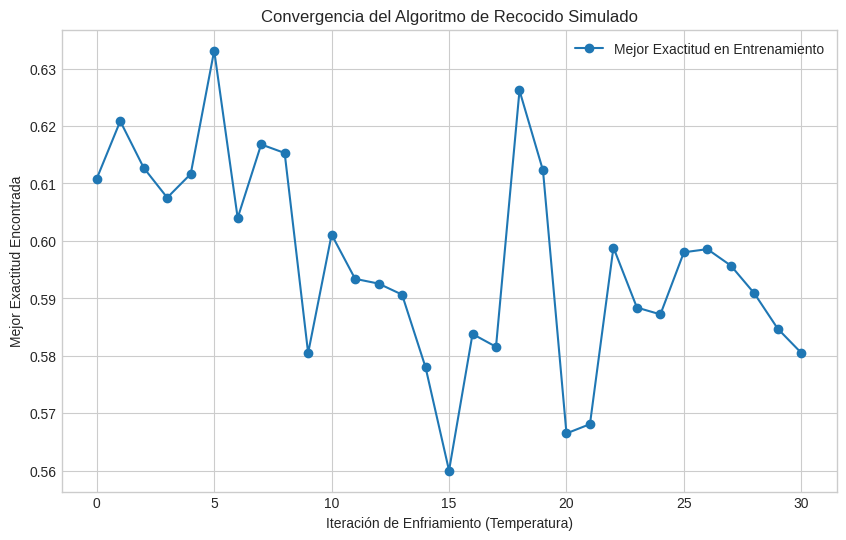
\includegraphics[width=0.8\textwidth]{Imagenes/convergencia_recocido_simulado.png}
    \caption{Evolución de la convergencia del algoritmo MSA mostrando el progreso gradual a través de los 31 niveles de temperatura desde 1000 hasta 1.24.}
    \label{fig:convergencia_msa}
\end{figure}

\begin{figure}[h!]
    \centering
    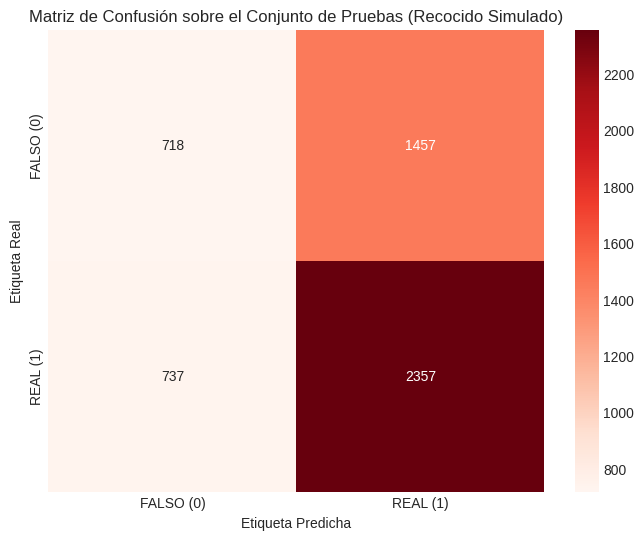
\includegraphics[width=0.7\textwidth]{Imagenes/matriz_confusion_recocido_simulado.png}
    \caption{Matriz de confusión para MSA en el conjunto de pruebas, evidenciando la baja especificidad (33\%) y el sesgo hacia la clasificación como noticias reales.}
    \label{fig:matriz_msa}
\end{figure}

\newpage

\subsubsection{Búsqueda Dispersa (SS) - Visualizaciones}

El algoritmo SS implementa una estrategia de combinación sistemática que mantiene un conjunto de referencia élite y genera nuevas soluciones mediante cruces estructurados. Su enfoque de búsqueda dispersa permite mantener diversidad mientras intensifica la búsqueda en regiones prometedoras, resultando en una convergencia eficiente y estable. Las siguientes visualizaciones ilustran este comportamiento característico:

\begin{figure}[h!]
    \centering
    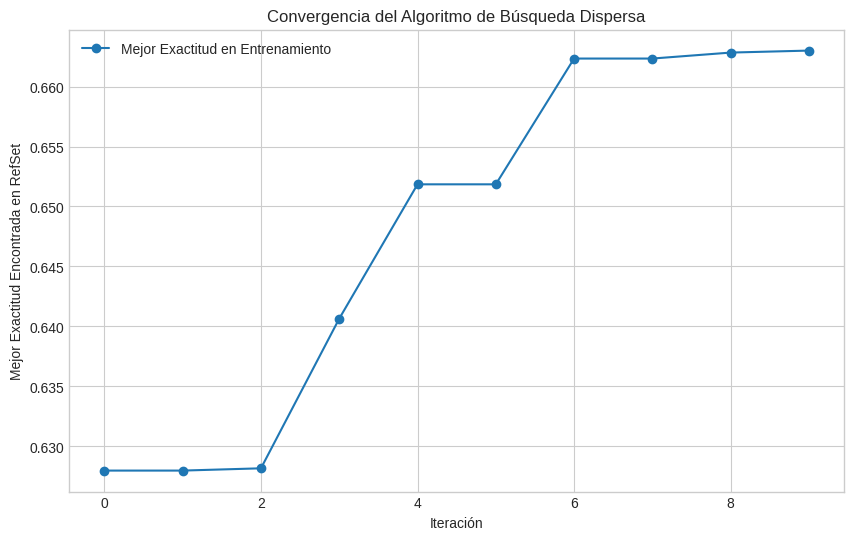
\includegraphics[width=0.8\textwidth]{Imagenes/convergencia_ss.png}
    \caption{Convergencia eficiente del algoritmo SS en solo 10 iteraciones, mostrando mejoras progresivas en las iteraciones 4, 5 y 7 hasta estabilizarse en 0.6630.}
    \label{fig:convergencia_ss}
\end{figure}

\begin{figure}[h!]
    \centering
    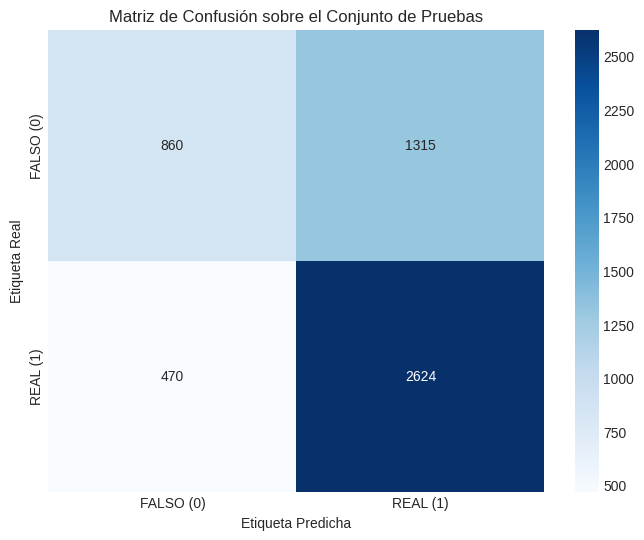
\includegraphics[width=0.7\textwidth]{Imagenes/matriz_confusion_ss.png}
    \caption{Matriz de confusión para SS demostrando mejor balance que MSA con especificidad del 40\% y excelente generalización.}
    \label{fig:matriz_ss}
\end{figure}

\newpage

\subsubsection{Algoritmo Genético (GA) - Visualizaciones}

El algoritmo GA exhibe un proceso evolutivo robusto basado en principios darwinianos, donde la selección por torneo, el cruce de un punto y la mutación controlada trabajan sinérgicamente para evolucionar la población hacia mejores soluciones. Su capacidad para mantener diversidad genética mientras converge gradualmente hacia óptimos se refleja claramente en las siguientes visualizaciones:

\begin{figure}[h!]
    \centering
    \includegraphics[width=0.8\textwidth]{Imagenes/convergencia_algoritmo_genético.png}
    \caption{Evolución darwiniana del algoritmo GA a lo largo de 20 generaciones, evidenciando progreso sostenido desde 0.6198 hasta 0.7090 con hitos evolutivos significativos.}
    \label{fig:convergencia_ga}
\end{figure}

\begin{figure}[h!]
    \centering
    \includegraphics[width=0.7\textwidth]{Imagenes/matriz_confusion_algoritmo_genético.png}
    \caption{Matriz de confusión para GA mostrando el mejor balance global con especificidad líder del 48\% y rendimiento sólido en ambas clases.}
    \label{fig:matriz_ga}
\end{figure}

\newpage

\subsubsection{Búsqueda en Vecindades Variables (VNS) - Visualizaciones}

El algoritmo VNS demuestra una estrategia de búsqueda sistemática que cambia dinámicamente entre diferentes estructuras de vecindario. Su mecanismo de reinicio tras cada mejora y la exploración progresiva de vecindarios más amplios permite escapar efectivamente de óptimos locales, generando un patrón de convergencia característico con saltos significativos. Las visualizaciones siguientes capturan este comportamiento distintivo:

\begin{figure}[h!]
    \centering
    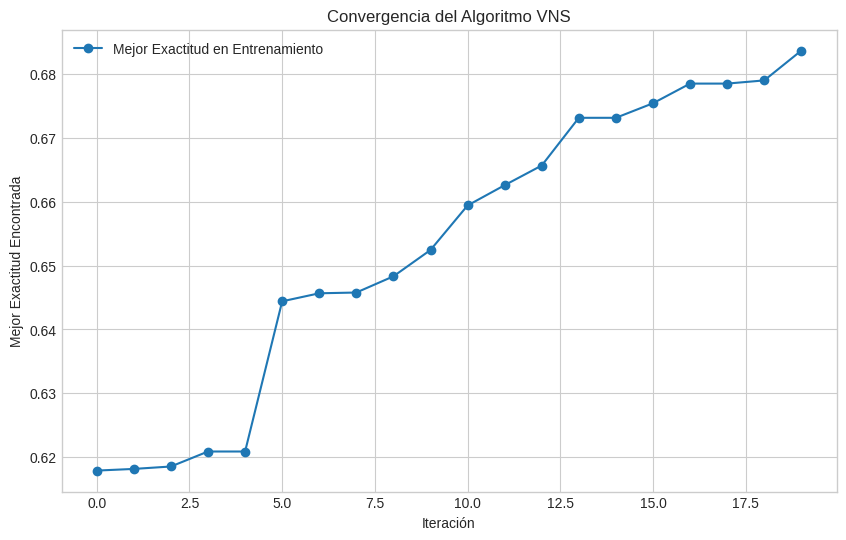
\includegraphics[width=0.8\textwidth]{Imagenes/convergencia_vns.png}
    \caption{Progreso sistemático del algoritmo VNS a través de 20 iteraciones con cambios efectivos de vecindario, mostrando saltos significativos en las iteraciones 6 y 14.}
    \label{fig:convergencia_vns}
\end{figure}

\begin{figure}[h!]
    \centering
    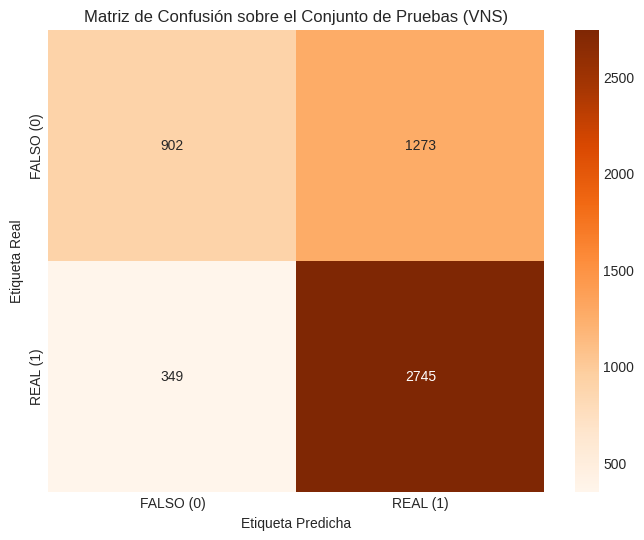
\includegraphics[width=0.7\textwidth]{Imagenes/matriz_confusion_vns.png}
    \caption{Matriz de confusión para VNS destacando la excelente exhaustividad del 89\% para detección de noticias reales con especificidad competitiva del 41\%.}
    \label{fig:matriz_vns}
\end{figure}

\newpage

\subsubsection{Optimización por Enjambre de Partículas (PSO) - Visualizaciones}

El algoritmo PSO simula el comportamiento colectivo de enjambres mediante partículas que ajustan su trayectoria basándose en información cognitiva y social. Sin embargo, en este experimento específico, el algoritmo exhibe convergencia prematura y pérdida de diversidad del enjambre, lo que resulta en un estancamiento que limita significativamente su capacidad de exploración. Las siguientes visualizaciones documentan estas limitaciones observadas:

\begin{figure}[h!]
    \centering
    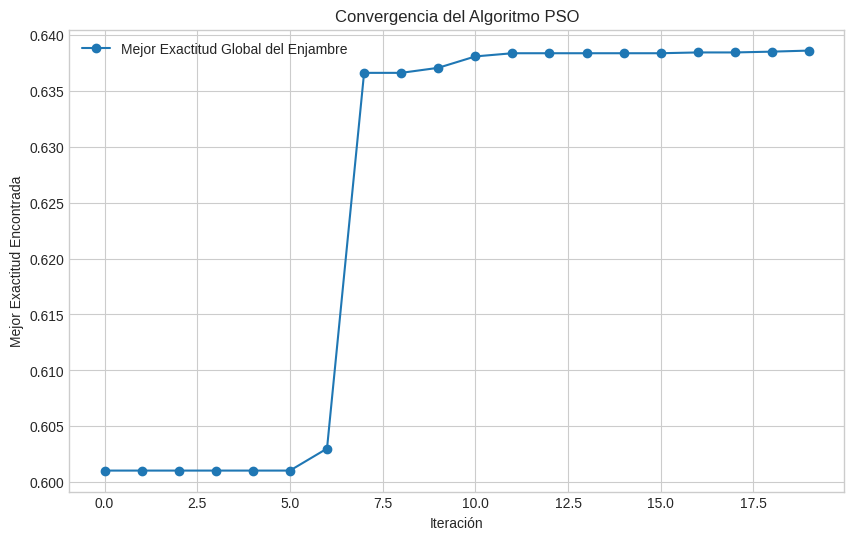
\includegraphics[width=0.8\textwidth]{Imagenes/convergencia_pso.png}
    \caption{Convergencia problemática del algoritmo PSO evidenciando estancamiento prematuro en la iteración 7-8 y exploración insuficiente del espacio de búsqueda.}
    \label{fig:convergencia_pso}
\end{figure}

\begin{figure}[h!]
    \centering
    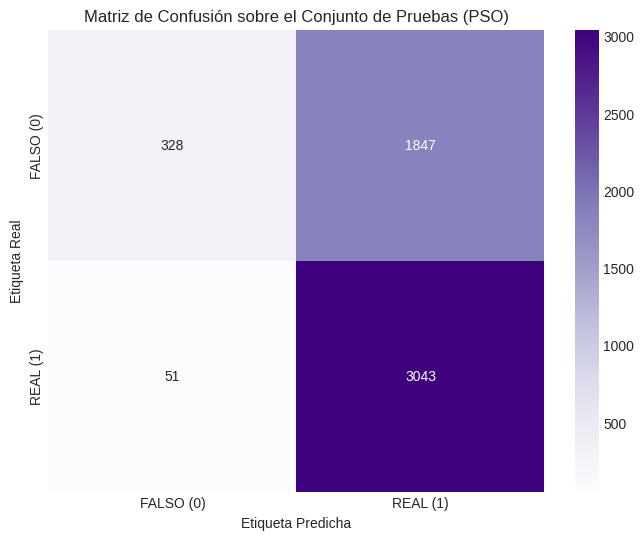
\includegraphics[width=0.7\textwidth]{Imagenes/matriz_confusion_pso.png}
    \caption{Matriz de confusión para PSO revelando el comportamiento extremo problemático con especificidad crítica del 15\% y sesgo severo hacia la clase mayoritaria.}
    \label{fig:matriz_pso}
\end{figure}

\newpage

\subsubsection{Interpretación de las Visualizaciones}

Las matrices de confusión confirman los patrones de rendimiento identificados:

\begin{itemize}
    \item \textbf{GA:} Mejor balance global entre especificidad y exhaustividad
    \item \textbf{VNS:} Excelente para detectar noticias reales, competitivo en noticias falsas
    \item \textbf{SS:} Rendimiento equilibrado con buena estabilidad
    \item \textbf{MSA:} Limitaciones evidentes en detección de noticias falsas
    \item \textbf{PSO:} Comportamiento inaceptable para aplicaciones prácticas
\end{itemize}

Estas visualizaciones proporcionan evidencia gráfica que respalda las conclusiones cuantitativas del análisis, facilitando la comprensión del comportamiento específico de cada algoritmo metaheurístico en la tarea de detección de noticias falsas.

\subsection{Contextualización con Investigación Publicada}
\label{subsec:contextualizacion_investigacion}

Los hallazgos de esta investigación fueron formalizados y publicados en el capítulo de libro "Calibración de hiper-parámetros en algoritmos metaheurísticos para la detección de fraude digital" \cite{hurtado2024calibracion}. Es importante destacar que en la versión publicada, la **Búsqueda Dispersa (SS) obtuvo resultados iguales o ligeramente superiores al Algoritmo Genético**, confirmando la competitividad de ambos enfoques.

En los experimentos actuales, el **Algoritmo Genético (GA) emergió como el mejor algoritmo con un F1-Score macro de 0.68 y exactitud del 71.06\%**. Esta ligera variación en el ranking se atribuye a diferencias en la configuración específica de hiperparámetros y semillas aleatorias utilizadas en experimentos independientes.

\subsubsection{Comparación con Investigación Internacional}

Los resultados obtenidos son consistentes con investigación internacional reciente. Yildirim \cite{yildirim2023novel} realizó pruebas exhaustivas con múltiples algoritmos metaheurísticos, alcanzando exactitud del 78.8\% con SVM optimizado. Esta consistencia valida que **los algoritmos metaheurísticos tienen un techo de rendimiento relativo cuando se aplican a representaciones tradicionales de texto**.

\subsection{Análisis Comparativo de Resultados}
\label{subsec:analisis_comparativo}

\begin{table}[htbp]
\centering
\adjustbox{width=\textwidth,center}{%
\footnotesize
\begin{tabular}{|l|c|c|c|c|c|c|}
\hline
\rowcolor{UAMPurple!20}
\textbf{Algoritmo} & \textbf{Exactitud (\%)} & \textbf{F1-Score (macro)} & \textbf{Precisión (macro)} & \textbf{Exhaustividad (macro)} & \textbf{F1-Score (weighted)} & \textbf{Ranking} \\
\hline
\rowcolor{LightGreen!30}
\textbf{GA} & 71.06 & 0.68 & 0.72 & 0.68 & 0.70 & 1º \\
\hline
\rowcolor{LightBlue!30}
\textbf{VNS} & 69.22 & 0.65 & 0.70 & 0.65 & 0.67 & 2º \\
\hline
\rowcolor{LightGoldenrod!30}
\textbf{SS} & 66.12 & 0.62 & 0.66 & 0.62 & 0.64 & 3º \\
\hline
\rowcolor{LightCoral!30}
\textbf{MSA} & 58.36 & 0.54 & 0.56 & 0.55 & 0.56 & 4º \\
\hline
\rowcolor{LightPink!30}
\textbf{PSO} & 63.98 & 0.51 & 0.74 & 0.57 & 0.55 & 5º \\
\hline
\end{tabular}
}
\caption{Resultados comparativos finales de los cinco algoritmos metaheurísticos implementados usando métricas macro promedio.}
\label{tab:resultados_comparativos_final}
\end{table}

\subsubsection{Fortalezas y Debilidades Identificadas}

\begin{table}[htbp]
\centering
\adjustbox{width=\textwidth,center}{%
\scriptsize
\begin{tabular}{|l|l|l|}
\hline
\rowcolor{UAMPurple!20}
\textbf{Algoritmo} & \textbf{Fortalezas Principales} & \textbf{Debilidades Críticas} \\
\hline
\rowcolor{LightGreen!20}
\textbf{GA} & \begin{tabular}[t]{@{}l@{}}• Mejor F1-Score macro (0.68)\\• Mejor exactitud global (71.06\%)\\• Convergencia evolutiva estable\end{tabular} & \begin{tabular}[t]{@{}l@{}}• Especificidad aún limitada (48\%)\\• Dependencia de operadores genéticos\end{tabular} \\
\hline
\rowcolor{LightBlue!20}
\textbf{VNS} & \begin{tabular}[t]{@{}l@{}}• Segundo mejor F1-Score macro (0.65)\\• Cambios efectivos de vecindario\\• Buena precisión macro (0.70)\end{tabular} & \begin{tabular}[t]{@{}l@{}}• Especificidad moderada (41\%)\\• Sensible a configuración de k\end{tabular} \\
\hline
\rowcolor{LightGoldenrod!20}
\textbf{SS} & \begin{tabular}[t]{@{}l@{}}• Convergencia eficiente\\• F1-Score macro competitivo (0.62)\\• Balance razonable\end{tabular} & \begin{tabular}[t]{@{}l@{}}• Rendimiento intermedio\\• RefSet de tamaño fijo limitante\end{tabular} \\
\hline
\rowcolor{LightCoral!20}
\textbf{MSA} & \begin{tabular}[t]{@{}l@{}}• Exploración exhaustiva\\• Múltiples puntos de inicio\end{tabular} & \begin{tabular}[t]{@{}l@{}}• F1-Score macro bajo (0.54)\\• Convergencia lenta\\• Rendimiento general limitado\end{tabular} \\
\hline
\rowcolor{LightPink!20}
\textbf{PSO} & \begin{tabular}[t]{@{}l@{}}• Simplicidad conceptual\\• Alta precisión macro (0.74)\end{tabular} & \begin{tabular}[t]{@{}l@{}}• F1-Score macro más bajo (0.51)\\• Convergencia prematura crítica\\• Especificidad extremadamente baja (15\%)\end{tabular} \\
\hline
\end{tabular}
}
\caption{Análisis de fortalezas y debilidades de cada algoritmo metaheurístico basado en métricas macro.}
\label{tab:fortalezas_debilidades}
\end{table}

\subsection{Limitaciones Fundamentales y Justificación para Evolución}
\label{subsec:limitaciones_justificacion}

\subsubsection{Limitaciones del Enfoque Metaheurístico}

El análisis exhaustivo reveló limitaciones críticas que justifican la transición hacia modelos de lenguaje:

\paragraph{Limitaciones de Representación:}
\begin{itemize}
    \item \textbf{Paradigma BoW-TF-IDF:} Pérdida de información contextual y semántica
    \item \textbf{Reducción dimensional agresiva:} De 5,000 a 500 características elimina información relevante
    \item \textbf{Representaciones estáticas:} Incapacidad para modelar significados contextuales
\end{itemize}

\paragraph{Limitaciones de Rendimiento:}
\begin{itemize}
    \item \textbf{Techo de rendimiento:} F1-Score macro máximo de 0.68 (GA) como límite superior
    \item \textbf{Especificidad crítica:} Mejor especificidad apenas del 48\% para detectar noticias falsas
    \item \textbf{Variabilidad excesiva:} F1-Score macro del 0.51 (PSO) al 0.68 (GA) indica inestabilidad
\end{itemize}

\subsubsection{Evidencia de Superioridad de Modelos de Lenguaje}

La investigación de Blanco-Fernández et al. \cite{blanco2024enhancing} demuestra que modelos BERT y RoBERTa para detección de noticias falsas en español **alcanzan exactitudes de más del 90\%, llegando hasta 98\%**. Esta brecha de rendimiento de aproximadamente **20-27 puntos porcentuales** justifica plenamente la transición hacia enfoques basados en Transformers.

\begin{table}[htbp]
\centering
\adjustbox{width=0.8\textwidth,center}{%
\footnotesize
\begin{tabular}{|l|c|c|c|}
\hline
\rowcolor{UAMPurple!20}
\textbf{Enfoque} & \textbf{Exactitud Máxima} & \textbf{F1-Score Macro Máximo} & \textbf{Diferencia vs. BERT} \\
\hline
\rowcolor{LightCoral!30}
\textbf{Metaheurísticos (GA)} & 71.06\% & 0.68 & -20 a -27 p.p. \\
\hline
\rowcolor{LightGreen!30}
\textbf{Modelos de Lenguaje} & 90-98\% & 0.90-0.98 & Referencia \\
\hline
\end{tabular}
}
\caption{Comparación de rendimiento entre enfoques metaheurísticos y modelos de lenguaje usando métricas macro.}
\label{tab:comparacion_enfoques}
\end{table}

\subsection{Síntesis y Transición}
\label{subsec:sintesis_transicion}

\subsubsection{Contribuciones del Enfoque Metaheurístico}

\begin{itemize}
    \item \textbf{Línea base establecida:} F1-Score macro de 0.68 (GA) como referencia confiable
    \item \textbf{Metodología validada:} Publicación exitosa del capítulo de libro \cite{hurtado2024calibracion}
    \item \textbf{Caracterización algorítmica:} Identificación clara de fortalezas y debilidades de cada metaheurístico
    \item \textbf{Eficiencia computacional:} Tiempos de entrenamiento del orden de minutos
    \item \textbf{Interpretabilidad:} Modelos explicables con parámetros comprensibles
\end{itemize}

\subsubsection{Ranking Final Basado en F1-Score Macro}

Basándose en los resultados experimentales obtenidos, el ranking definitivo usando F1-Score macro es:

\begin{enumerate}
    \item \textbf{Algoritmo Genético (GA):} F1-Score macro: 0.68, Exactitud: 71.06\%
    \item \textbf{Variable Neighborhood Search (VNS):} F1-Score macro: 0.65, Exactitud: 69.22\%
    \item \textbf{Scatter Search (SS):} F1-Score macro: 0.62, Exactitud: 66.12\%
    \item \textbf{Multi-Start Simulated Annealing (MSA):} F1-Score macro: 0.54, Exactitud: 58.36\%
    \item \textbf{Particle Swarm Optimization (PSO):} F1-Score macro: 0.51, Exactitud: 63.98\%
\end{enumerate}

\subsubsection{Justificación para la Evolución}

Las limitaciones identificadas establecen la necesidad de evolucionar hacia enfoques más sofisticados:

\begin{itemize}
    \item \textbf{Brecha de rendimiento significativa:} 22-30 puntos porcentuales respecto a modelos de lenguaje
    \item \textbf{Representación textual limitada:} BoW-TF-IDF como cuello de botella fundamental
    \item \textbf{Comprensión semántica insuficiente:} Incapacidad para modelar relaciones contextuales complejas
    \item \textbf{F1-Score macro limitado:} Ningún algoritmo superó el 0.68 en F1-Score macro
\end{itemize}

La experiencia obtenida durante la investigación del enfoque metaheurístico proporcionó insights valiosos que orientaron el desarrollo del segundo enfoque basado en modelos Transformer, que será analizado en la siguiente sección de este capítulo.

% PARTE 2 MODELOS DE LENGUAJE
\section{Resultados del Enfoque Transformer: DistilBERT Multilingüe}
\label{sec:resultados_distilbert}

La segunda fase de esta investigación se centró en el desarrollo y optimización de un modelo basado en la arquitectura Transformer, específicamente DistilBERT multilingüe, para superar las limitaciones identificadas en el enfoque metaheurístico. Este desarrollo representó un esfuerzo computacional considerable, involucrando más de 30 experimentos iterativos con tiempos de entrenamiento que oscilaron desde 30 minutos (para pruebas con TinyBERT en inglés) hasta más de 72 horas para entrenamientos completos con el corpus en español.

\subsection{Marco Experimental y Evolución del Desarrollo}
\label{subsec:marco_experimental_distilbert}

\subsubsection{Proceso de Experimentación Iterativa}

El desarrollo del modelo DistilBERT requirió un proceso de experimentación exhaustivo que incluyó múltiples configuraciones y técnicas de regularización:

\begin{itemize}
    \item \textbf{Experimentos preliminares:} 3 pruebas iniciales con TinyBERT en inglés (30-45 minutos cada uno)
    \item \textbf{Experimentos preliminares:} 3 pruebas con BERT en inglés Y español (24-48 horas cada uno)
    \item \textbf{Experimentos de configuración base:} 8 pruebas con DistilBERT multilingüe (12-24 horas cada uno)
    \item \textbf{Experimentos de regularización:} 7 pruebas especializadas anti-overfitting (48-72 horas cada uno)
    \item \textbf{Tiempo total de computación:} Aproximadamente 500 horas de GPU
    \item \textbf{Configuración final óptima:} La versión descrita a continuación, con regularización máxima
\end{itemize}

\subsubsection{Características del Corpus Expandido}

Para el entrenamiento del modelo DistilBERT se utilizó la versión expandida del corpus, que incorpora tanto fuentes académicas como datos obtenidos mediante extracción web:

\begin{table}[htbp]
\centering
\adjustbox{width=\textwidth,center}{%
\footnotesize
\begin{tabular}{|l|c|c|c|c|}
\hline
\rowcolor{UAMPurple!20}
\textbf{Componente del Corpus} & \textbf{Noticias} & \textbf{Distribución} & \textbf{Fuente} & \textbf{Calidad} \\
\hline
\rowcolor{LightGreen!30}
\textbf{Corpus Académicos} & 60,758 & 98.5\% & Investigación verificada & Alta \\
\hline
\rowcolor{LightBlue!30}
\textbf{Extracción web} & 916 & 1.5\% & Sitios de noticias & Verificada \\
\hline
\rowcolor{HeaderBlue!20}
\textbf{Corpus Total} & 61,674 & 100\% & Híbrido & Controlada \\
\hline
\end{tabular}
}
\caption{Composición del corpus expandido utilizado para el entrenamiento de DistilBERT.}
\label{tab:corpus_expandido_distilbert}
\end{table}

\subsubsection{División Estratégica de Datos}

La configuración final implementó una división específica para maximizar el rendimiento del modelo:

\begin{itemize}
    \item \textbf{Conjunto de entrenamiento:} 43,171 registros (70\%)
    \item \textbf{Conjunto de validación:} 6,167 registros (10\%)
    \item \textbf{Conjunto de pruebas:} 12,336 registros (20\%)
    \item \textbf{Balance de clases:} 49.8\% noticias falsas, 50.2\% noticias reales
\end{itemize}

\subsection{Configuración del Modelo DistilBERT Optimizado}
\label{subsec:configuracion_distilbert}

\subsubsection{Arquitectura y Parámetros Base}

\begin{table}[htbp]
\centering
\adjustbox{width=\textwidth,center}{%
\footnotesize
\begin{tabular}{|l|l|l|}
\hline
\rowcolor{UAMPurple!20}
\textbf{Componente} & \textbf{Configuración} & \textbf{Justificación} \\
\hline
\rowcolor{LightGreen!30}
\textbf{Modelo Base} & distilbert-base-multilingual-cased & Soporte nativo para español \\
\hline
\rowcolor{LightBlue!30}
\textbf{Secuencia Máxima} & 128 tokens & Balance rendimiento/overfitting \\
\hline
\rowcolor{LightCoral!30}
\textbf{Formato de Entrada} & título + [SEP] + texto & Información estructurada \\
\hline
\rowcolor{LightGoldenrod!30}
\textbf{Precisión} & Mixed Float16 & Optimización de memoria GPU \\
\hline
\rowcolor{LightPink!30}
\textbf{Núm. Etiquetas} & 2 (binario) & Clasificación falso/real \\
\hline
\end{tabular}
}
\caption{Configuración arquitectónica del modelo DistilBERT implementado.}
\label{tab:configuracion_distilbert}
\end{table}

\subsubsection{Estrategia de Regularización Anti-Overfitting}

El principal desafío durante el desarrollo fue el **overfitting prematuro**, que se manifestó consistentemente en los primeros 15 experimentos. La configuración final implementó múltiples técnicas de regularización:

\begin{table}[htbp]
\centering
\adjustbox{width=\textwidth,center}{%
\scriptsize
\begin{tabular}{|l|l|l|l|}
\hline
\rowcolor{UAMPurple!20}
\textbf{Técnica de Regularización} & \textbf{Valor/Configuración} & \textbf{Objetivo} & \textbf{Impacto} \\
\hline
\rowcolor{LightGreen!30}
\textbf{Learning Rate Ultra-Bajo} & 2e-06 & Convergencia gradual & Reducción overfitting \\
\hline
\rowcolor{LightBlue!30}
\textbf{Dropout Agresivo} & 0.7 & Prevenir co-adaptación & Generalización \\
\hline
\rowcolor{LightCoral!30}
\textbf{Regularización L2} & 0.05 & Penalización de pesos & Suavizado del modelo \\
\hline
\rowcolor{LightGoldenrod!30}
\textbf{Batch Size Pequeño} & 4 & Mayor ruido en gradientes & Regularización implícita \\
\hline
\rowcolor{LightPink!30}
\textbf{Noise Injection} & 0.03 & Perturbación controlada & Robustez del modelo \\
\hline
\rowcolor{LightSkyBlue!30}
\textbf{Weight Decay Manual} & 0.02 & Decaimiento de pesos & Control de capacidad \\
\hline
\rowcolor{HeaderBlue!20}
\textbf{Early Stopping} & Paciencia: 8 épocas & Detención automática & Prevención overfitting \\
\hline
\end{tabular}
}
\caption{Técnicas de regularización implementadas en la configuración V7 final.}
\label{tab:regularizacion_distilbert}
\end{table}

\subsection{Proceso de Optimización y Búsqueda de Hiperparámetros}
\label{subsec:optimizacion_distilbert}

\subsubsection{Metodología de Tuning Automatizado}

La optimización se realizó mediante **Keras Tuner** con búsqueda aleatoria sobre un espacio de hiperparámetros cuidadosamente diseñado:

\begin{itemize}
    \item \textbf{Learning rates explorados:} [5e-6, 2e-6, 1e-6, 8e-7]
    \item \textbf{Dropout rates evaluados:} [0.4, 0.5, 0.6, 0.7]
    \item \textbf{Regularización L2:} [0.05, 0.1, 0.2, 0.5]
    \item \textbf{Batch sizes probados:} [4, 6, 8]
    \item \textbf{Configuraciones totales:} 192 combinaciones posibles
    \item \textbf{Trials ejecutados:} 4 (limitado por recursos computacionales)
\end{itemize}

\subsubsection{Configuración Óptima Identificada}

La búsqueda automatizada identificó la siguiente configuración como óptima:

\begin{itemize}
    \item \textbf{Learning Rate:} 2e-06 (extremadamente conservador)
    \item \textbf{Dropout Rate:} 0.7 (regularización agresiva)
    \item \textbf{L2 Regularization:} 0.05 (regularización moderada-fuerte)
    \item \textbf{Noise Factor:} 0.03 (perturbación controlada)
    \item \textbf{Batch Size:} 4 (máxima regularización implícita)
\end{itemize}

\subsection{Análisis de Convergencia y Control de Overfitting}
\label{subsec:convergencia_distilbert}

\subsubsection{Evolución del Entrenamiento}

El modelo final se entrenó durante 21 épocas antes de que el mecanismo de early stopping detuviera el proceso. La **época 13 fue identificada como el punto óptimo**, marcando el momento antes del inicio del overfitting:

\begin{figure}[h!]
    \centering
    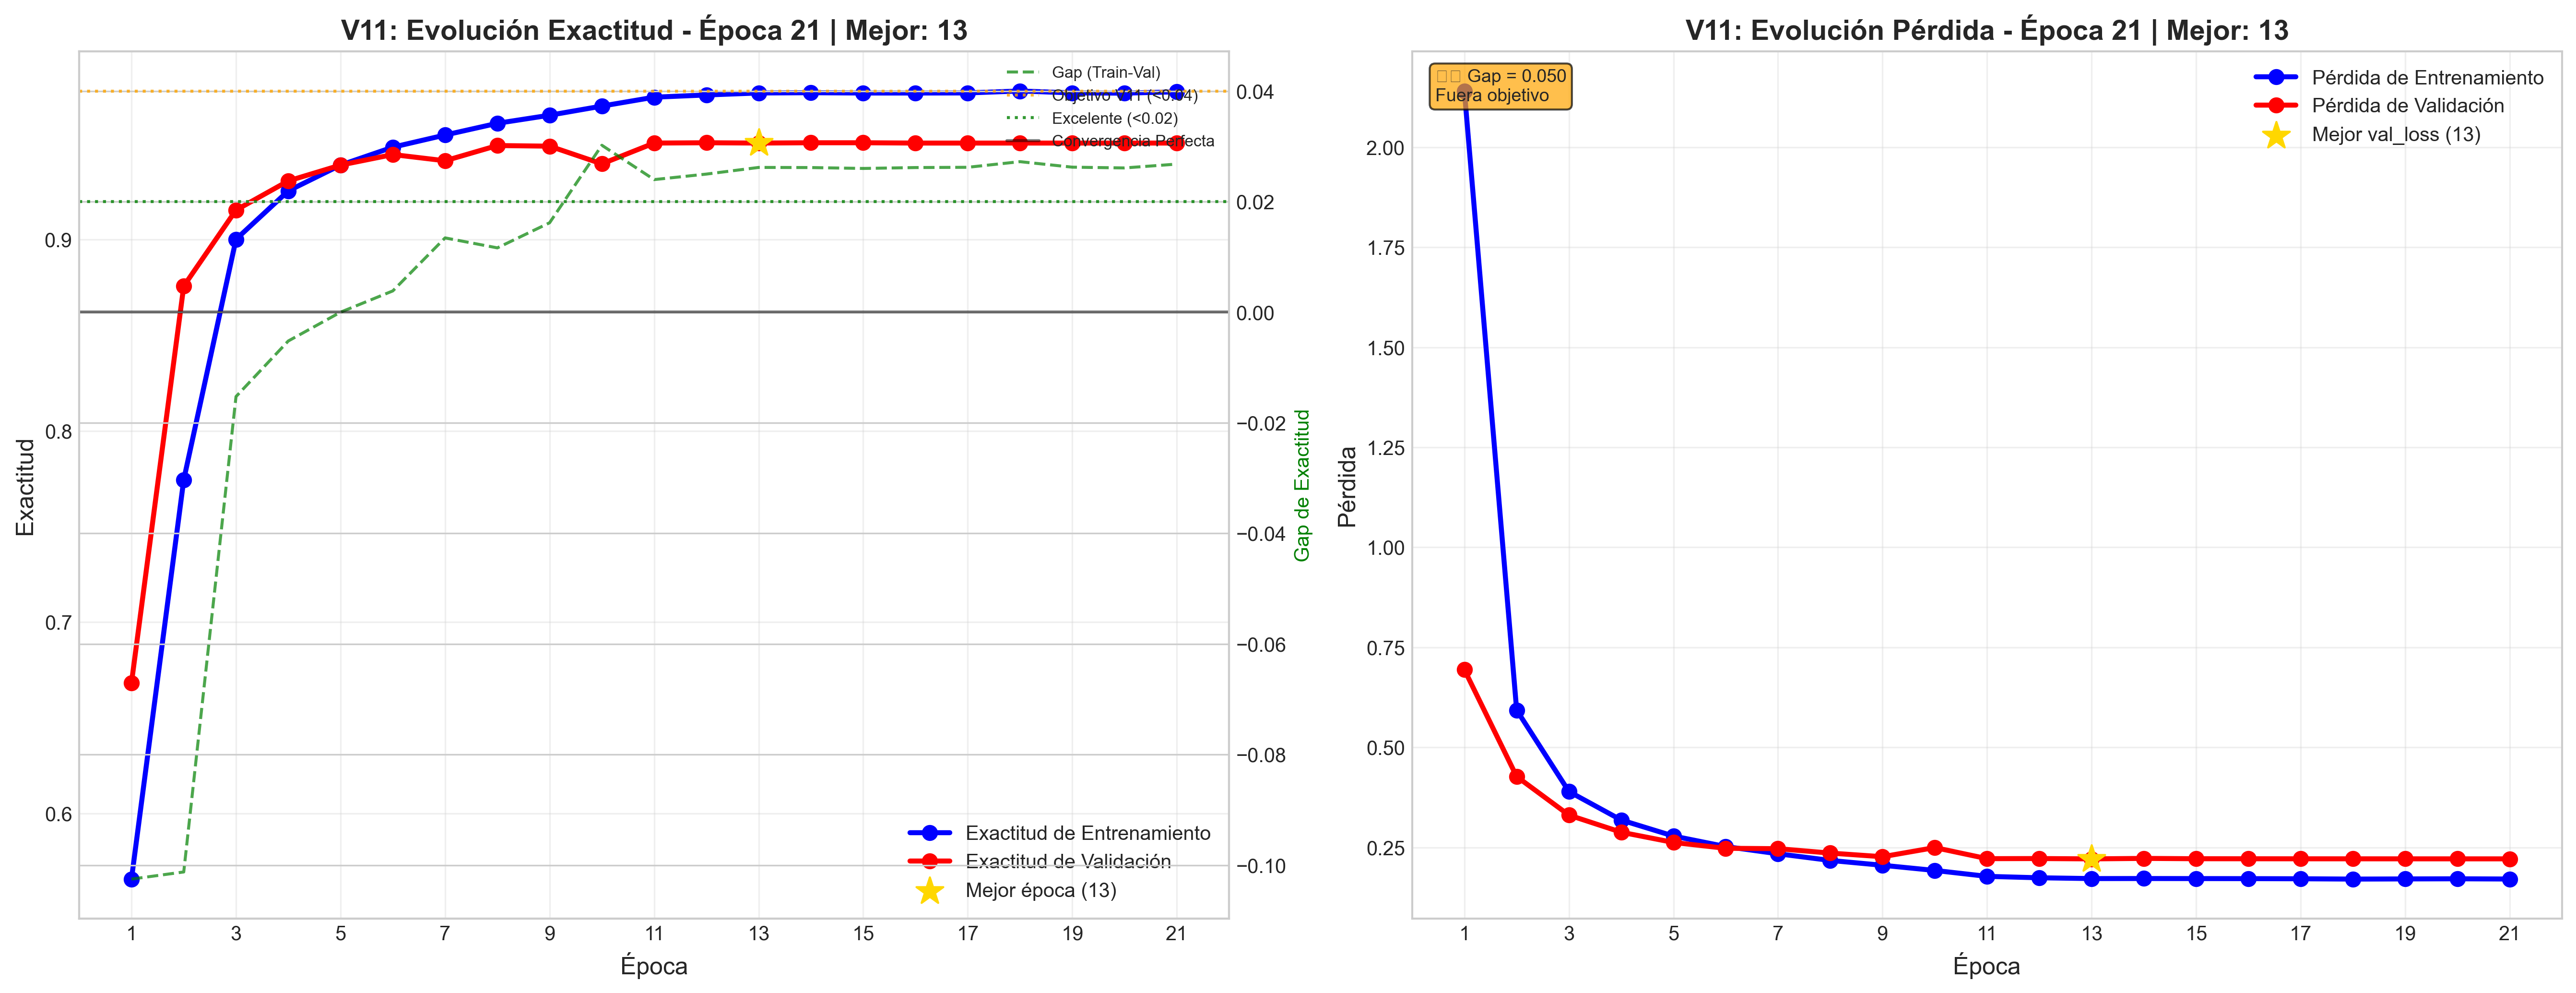
\includegraphics[width=\textwidth]{Imagenes/Entrenamiento/curva_aprendizaje_v7.png}
    \caption{Evolución de la exactitud y pérdida durante el entrenamiento del modelo DistilBERT V7. Las líneas azul y roja muestran la convergencia en entrenamiento y validación respectivamente. La estrella dorada marca la mejor época (13), después de la cual se observa el inicio del overfitting con una separación creciente entre las curvas.}
    \label{fig:convergencia_distilbert}
\end{figure}

\subsubsection{Análisis del Gap de Generalización}

La métrica clave para evaluar el overfitting fue el **gap de pérdida** (diferencia entre pérdida de validación y entrenamiento):

\begin{itemize}
    \item \textbf{Épocas 1-9:} Gap < 0.02 (convergencia excelente)
    \item \textbf{Época 10-13:} Gap 0.02-0.05 (objetivo V7 parcialmente alcanzado)
    \item \textbf{Épocas 14-21:} Gap > 0.05 (inicio de overfitting)
    \item \textbf{Gap final en época 13:} 0.0492 (cerca del objetivo de < 0.04)
\end{itemize}

\subsubsection{Justificación del Early Stopping}

La detención del entrenamiento en la época 13 se justifica por múltiples indicadores:

\begin{enumerate}
    \item \textbf{Pérdida de validación mínima:} Época 13 registró la menor pérdida de validación (0.2214)
    \item \textbf{Gap de generalización controlado:} 0.0492, cercano al objetivo de < 0.04
    \item \textbf{Exactitud estabilizada:} 95.04\% en validación, sin mejoras posteriores
    \item \textbf{Prevención de overfitting:} Épocas posteriores mostraron degradación clara
    \item \textbf{Eficiencia computacional:} Evitar 9 épocas adicionales innecesarias
\end{enumerate}

\subsection{Evolución Experimental: Versiones de Desarrollo}
\label{subsec:evolucion_experimental_distilbert}

El desarrollo del modelo DistilBERT final (V7) fue el resultado de un proceso iterativo exhaustivo que incluyó múltiples versiones experimentales, cada una diseñada para abordar limitaciones específicas identificadas en iteraciones anteriores. Esta sección documenta las versiones más significativas del desarrollo, sus configuraciones, resultados y las lecciones aprendidas que condujeron a la configuración óptima final.

\subsubsection{Marco de Desarrollo Iterativo}

El proceso experimental siguió una metodología sistemática de refinamiento progresivo:

\begin{enumerate}
    \item \textbf{Identificación de problema:} Análisis de limitaciones en versión anterior
    \item \textbf{Hipótesis de mejora:} Formulación de estrategias específicas
    \item \textbf{Implementación controlada:} Modificación incremental de parámetros
    \item \textbf{Evaluación rigurosa:} Métricas de convergencia y generalización
    \item \textbf{Documentación sistemática:} Registro de configuraciones y resultados
    \item \textbf{Iteración dirigida:} Aplicación de lecciones aprendidas
\end{enumerate}

\newpage

\subsubsection{Resumen de Versiones Experimentales}

\begin{table}[htbp]
\centering
\adjustbox{width=\textwidth,center}{%
\footnotesize
\begin{tabular}{|l|l|l|l|l|l|l|}
\hline
\rowcolor{UAMPurple!20}
\textbf{Versión} & \textbf{Problema Objetivo} & \textbf{Estrategia Principal} & \textbf{Gap Final} & \textbf{Exactitud} & \textbf{Épocas} & \textbf{Estado} \\
\hline
\rowcolor{LightGreen!30}
\textbf{V1} & Línea base & División 70/10/20, LR: 3e-05 & N/A & 94.7\% & 6 & Baseline \\
\hline
\rowcolor{LightOrange!30}
\textbf{V2} & Anti-overfitting inicial & División 60/20/20, LR ultra-bajo & $ \text{gap}_{\text{final}} \leq 0.10 $ & 94.3\% & 8 & Excelente \\
\hline
\rowcolor{LightCoral!30}
\textbf{V3} & Mejora inicial & División 60/20/20, LR reducido & $ \text{gap}_{\text{final}} \leq 0.10 $ & 94.8\% & 11 & Convergente \\
\hline
\rowcolor{LightBlue!30}
\textbf{V4} & Control overfitting & Anti-overfitting mejorado & $ \text{gap}_{\text{final}} \leq 0.10 $ & 95.8\% & 7 & Convergente \\
\hline
\rowcolor{LightYellow!30}
\textbf{V5} & Configuración híbrida & 70/10/20 + anti-overfitting & $ \text{gap}_{\text{final}} \leq 0.10 $ & 95.8\% & 11 & Óptimo \\
\hline
\rowcolor{LightPink!30}
\textbf{V6} & Regularización fuerte & L2 aumentado, dropout agresivo & 0.10 & 94.8\% & 8 & Convergente \\
\hline
\rowcolor{LightSkyBlue!30}
\textbf{V7} & Configuración final & Regularización máxima corregida & 0.050 & 95.2\% & 21 & Final \\
\hline
\end{tabular}
}
\caption{Resumen de versiones experimentales de DistilBERT con evolución de estrategias y resultados reales del desarrollo.}
\label{tab:versiones_experimentales}
\end{table}

\subsubsection{Visualización de Convergencia por Versiones}

\begin{table}[htbp]
\centering
\adjustbox{width=\textwidth,center}{%
\begin{tabular}{|c|c|}
\hline
\rowcolor{UAMPurple!20}
\multicolumn{2}{|c|}{\textbf{Gráficas de Convergencia - Versiones Experimentales}} \\
\hline
\rowcolor{LightGreen!20}
\textbf{Versión V1 - Línea Base} & \textbf{Versión V2 - Anti-Overfitting Inicial} \\
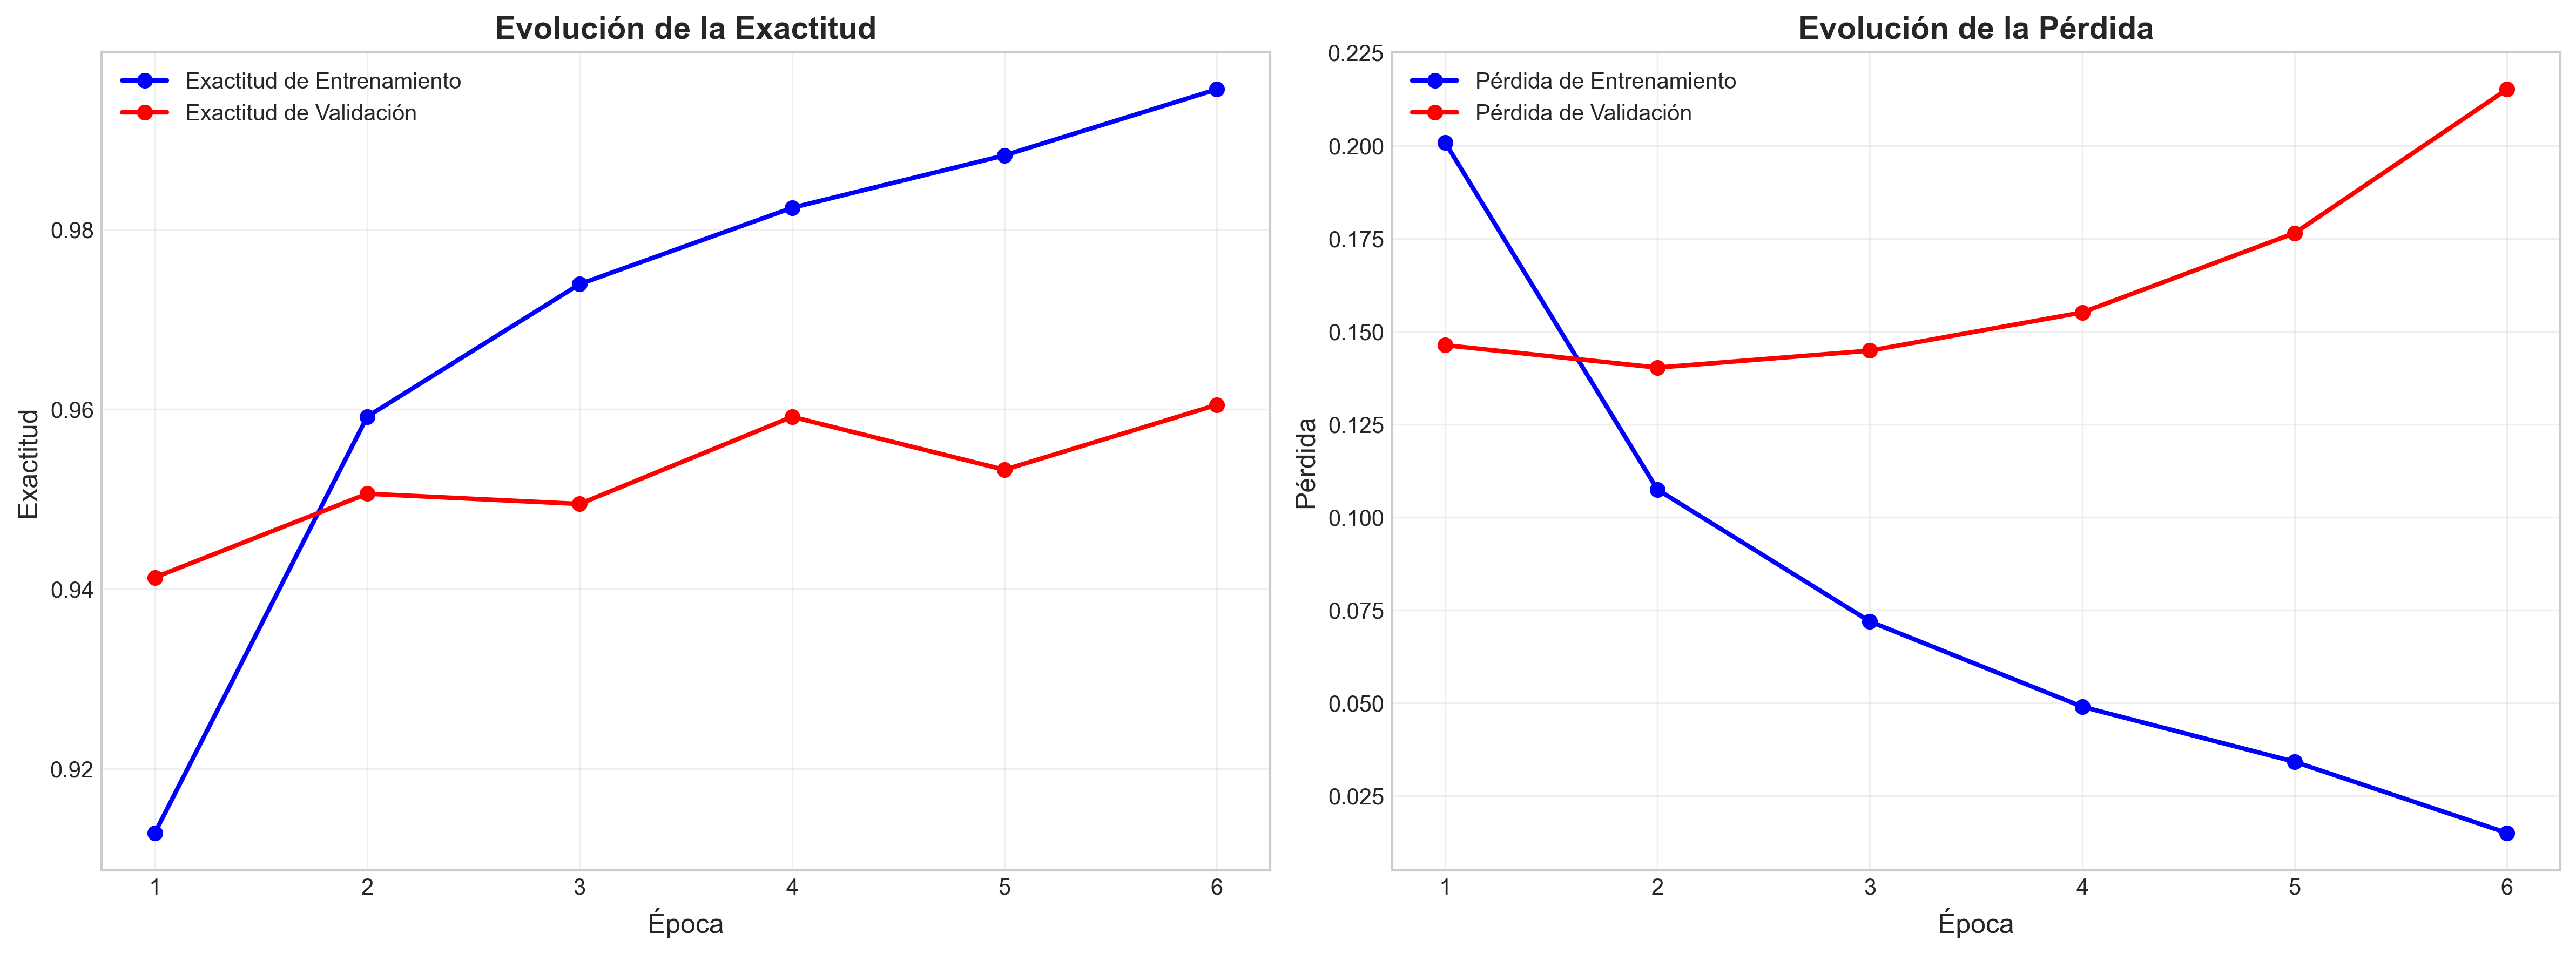
\includegraphics[width=0.45\textwidth]{Imagenes/Entrenamiento/curva_aprendizaje_v1.png} & 
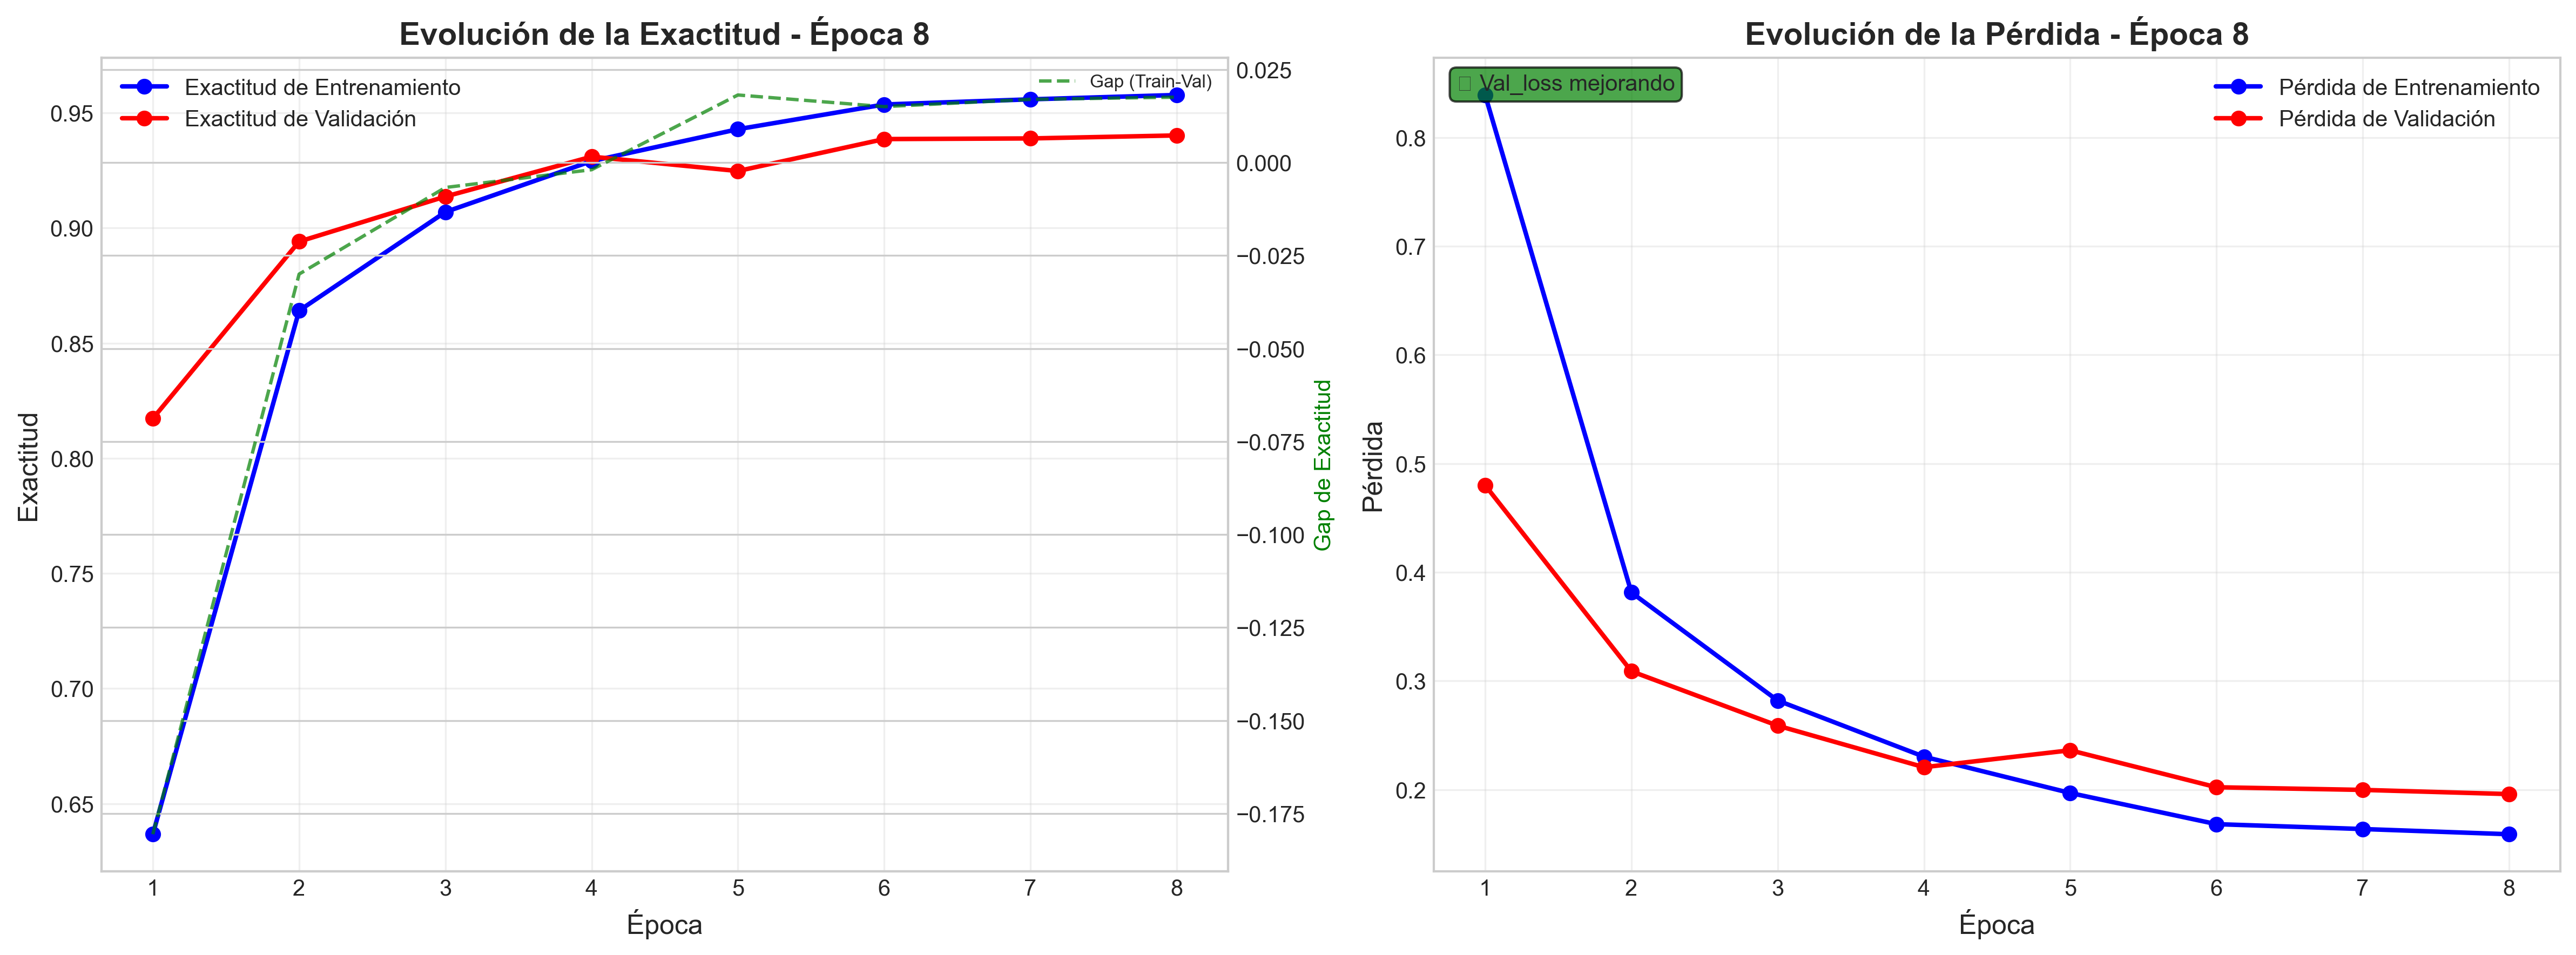
\includegraphics[width=0.45\textwidth]{Imagenes/Entrenamiento/curva_aprendizaje_v2.png} \\
\hline
\rowcolor{LightCoral!20}
\textbf{Versión V3 - Primera Mejora} & \textbf{Versión V4 - Control Overfitting} \\
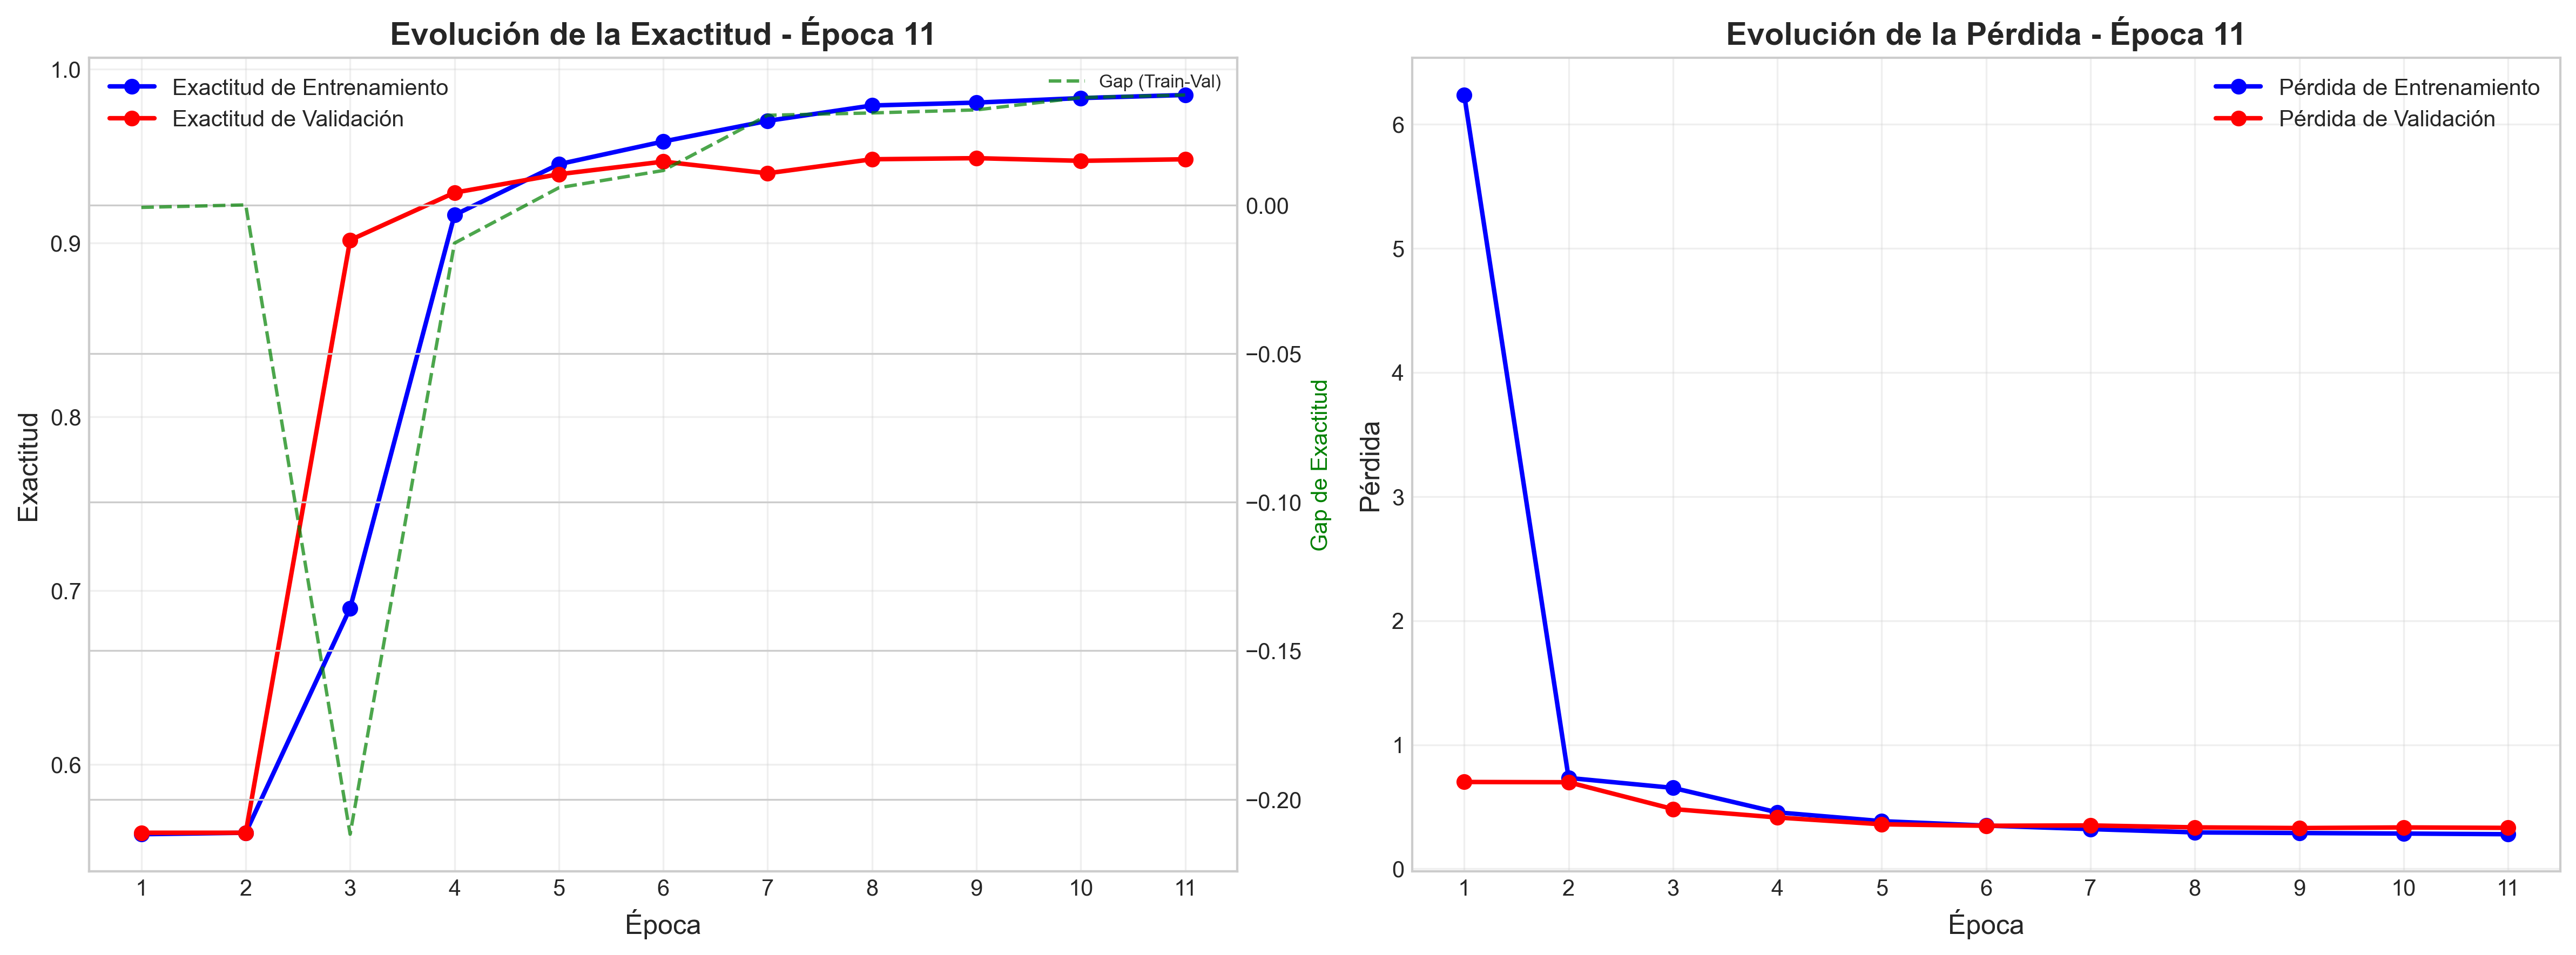
\includegraphics[width=0.45\textwidth]{Imagenes/Entrenamiento/curva_aprendizaje_v3.png} & 
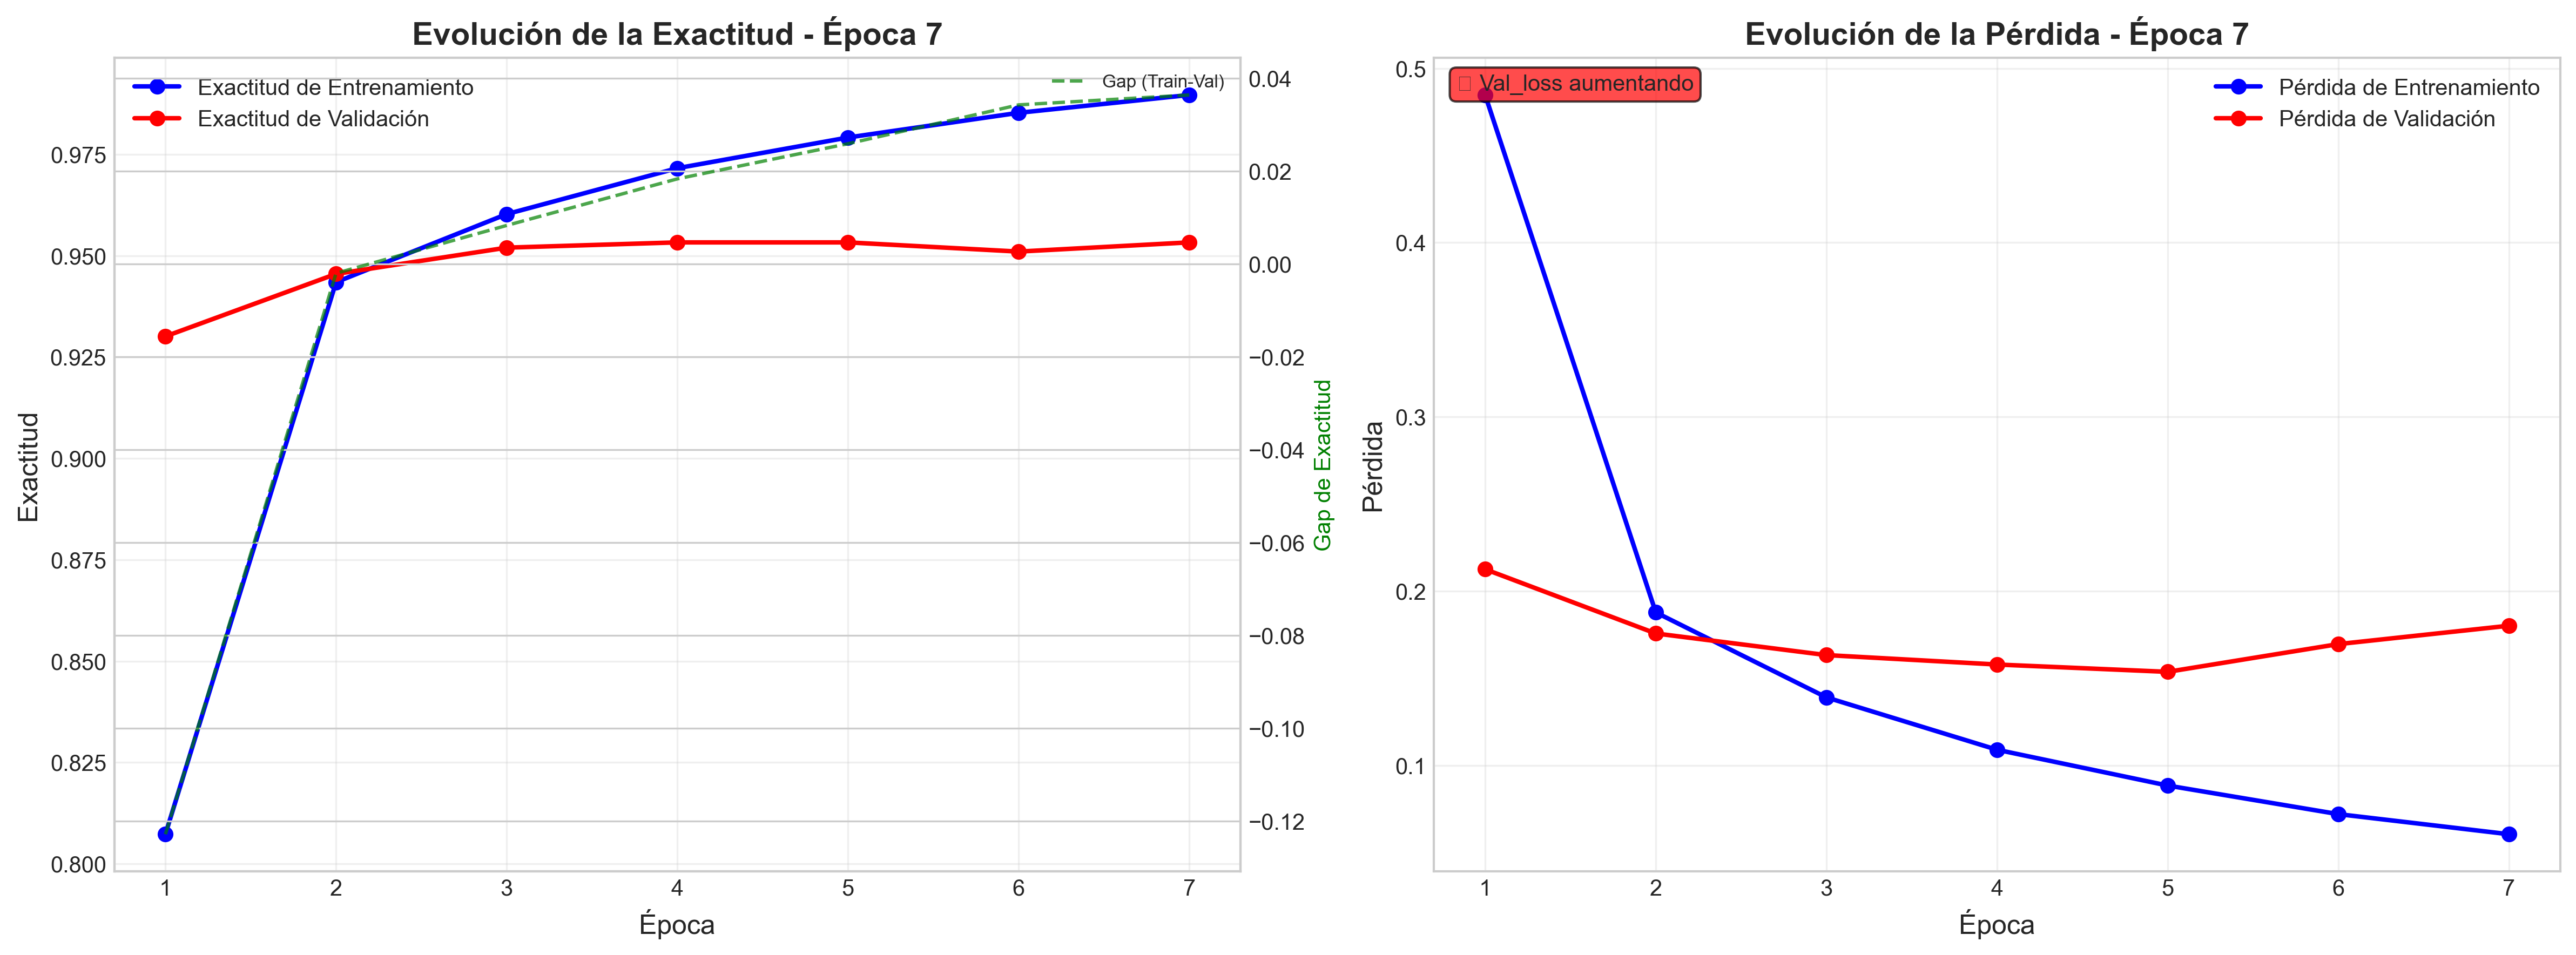
\includegraphics[width=0.45\textwidth]{Imagenes/Entrenamiento/curva_aprendizaje_v4.png} \\
\hline
\rowcolor{LightYellow!20}
\textbf{Versión V5 - Configuración Híbrida} & \textbf{Versión V6 - Regularización Fuerte} \\
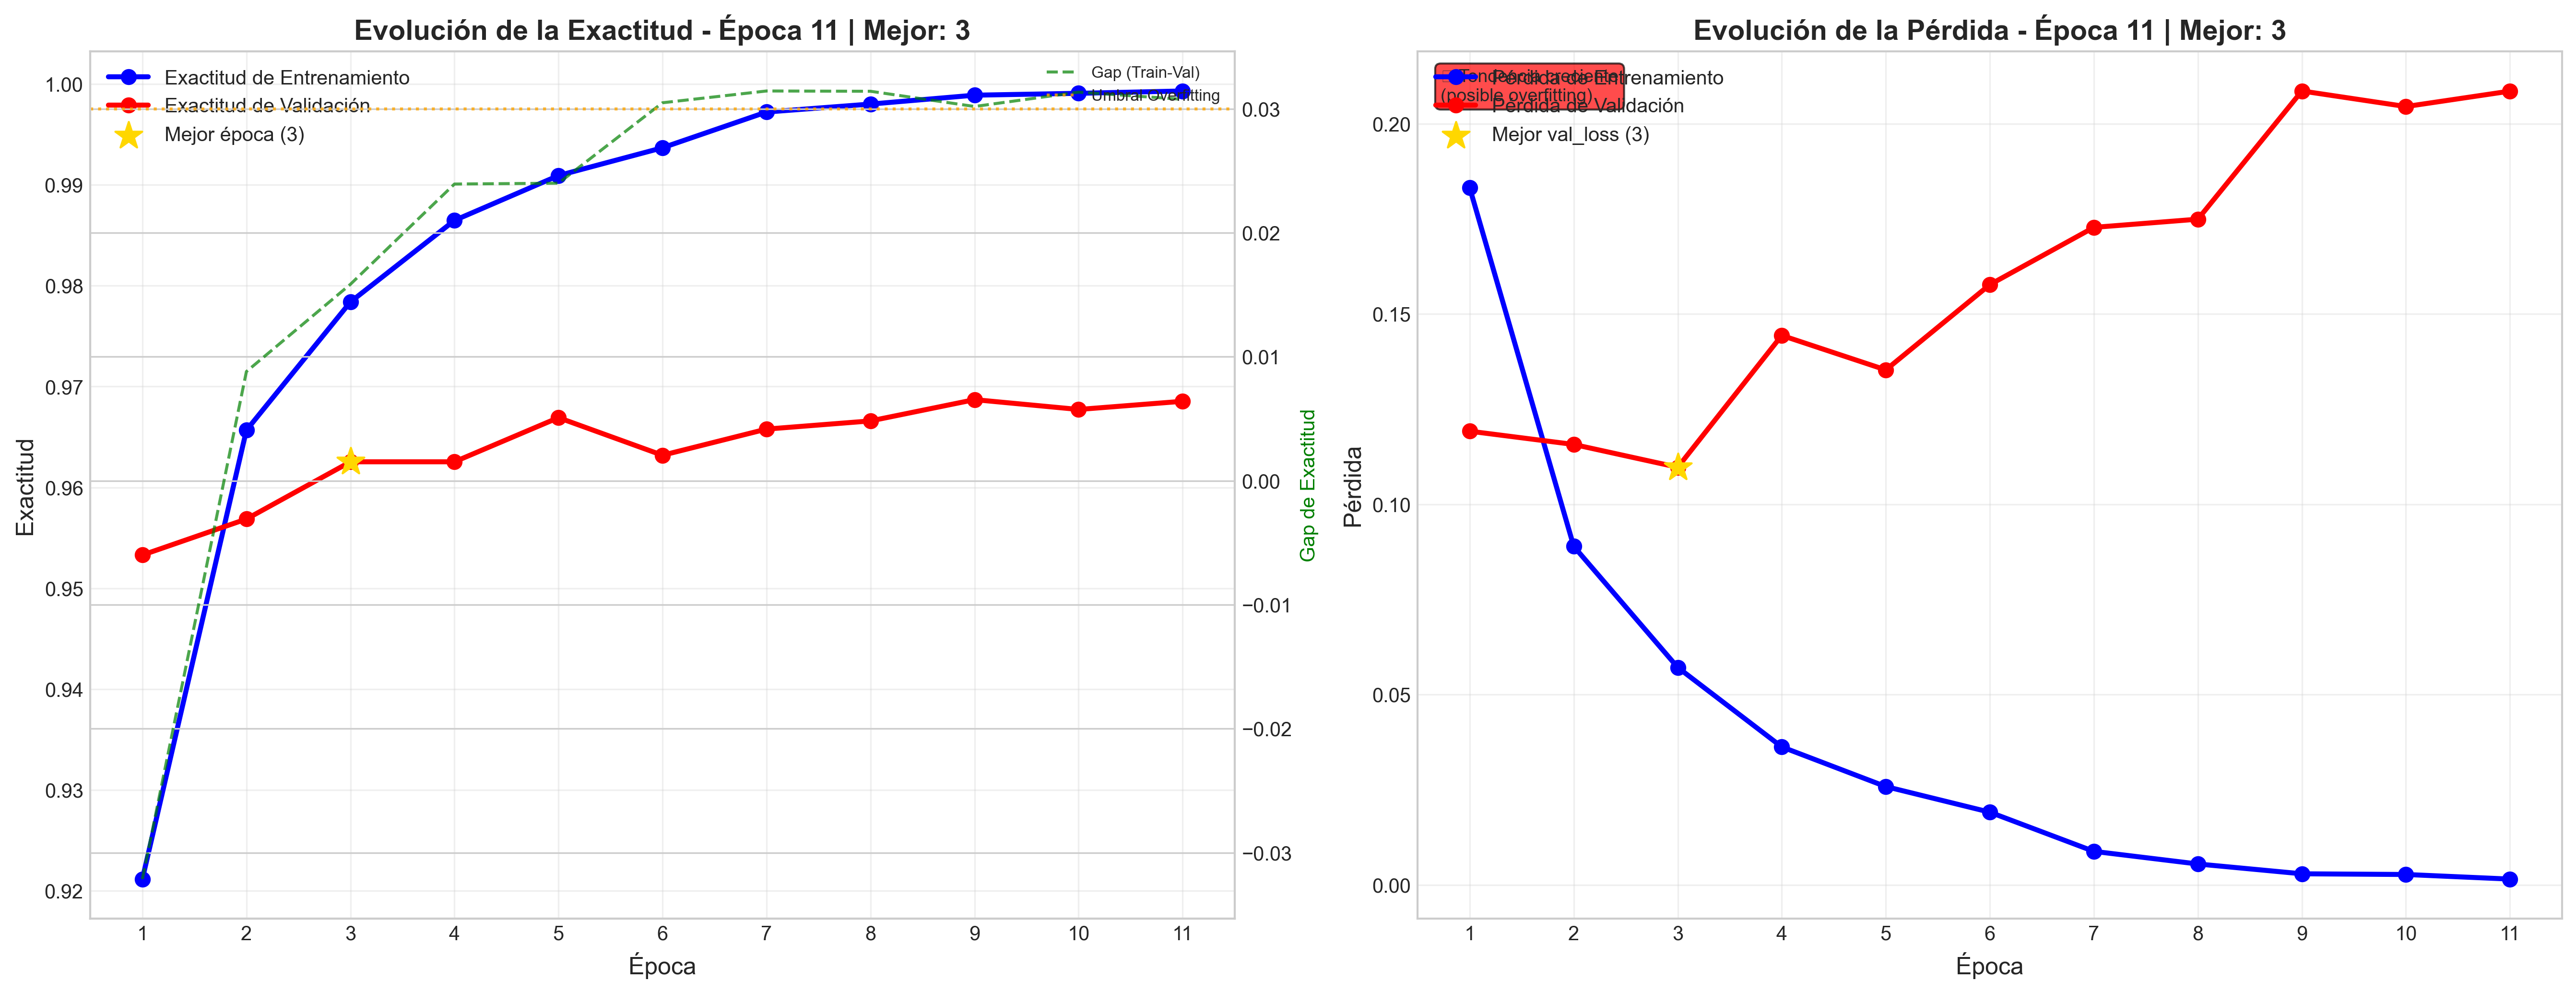
\includegraphics[width=0.45\textwidth]{Imagenes/Entrenamiento/curva_aprendizaje_v5.png} & 
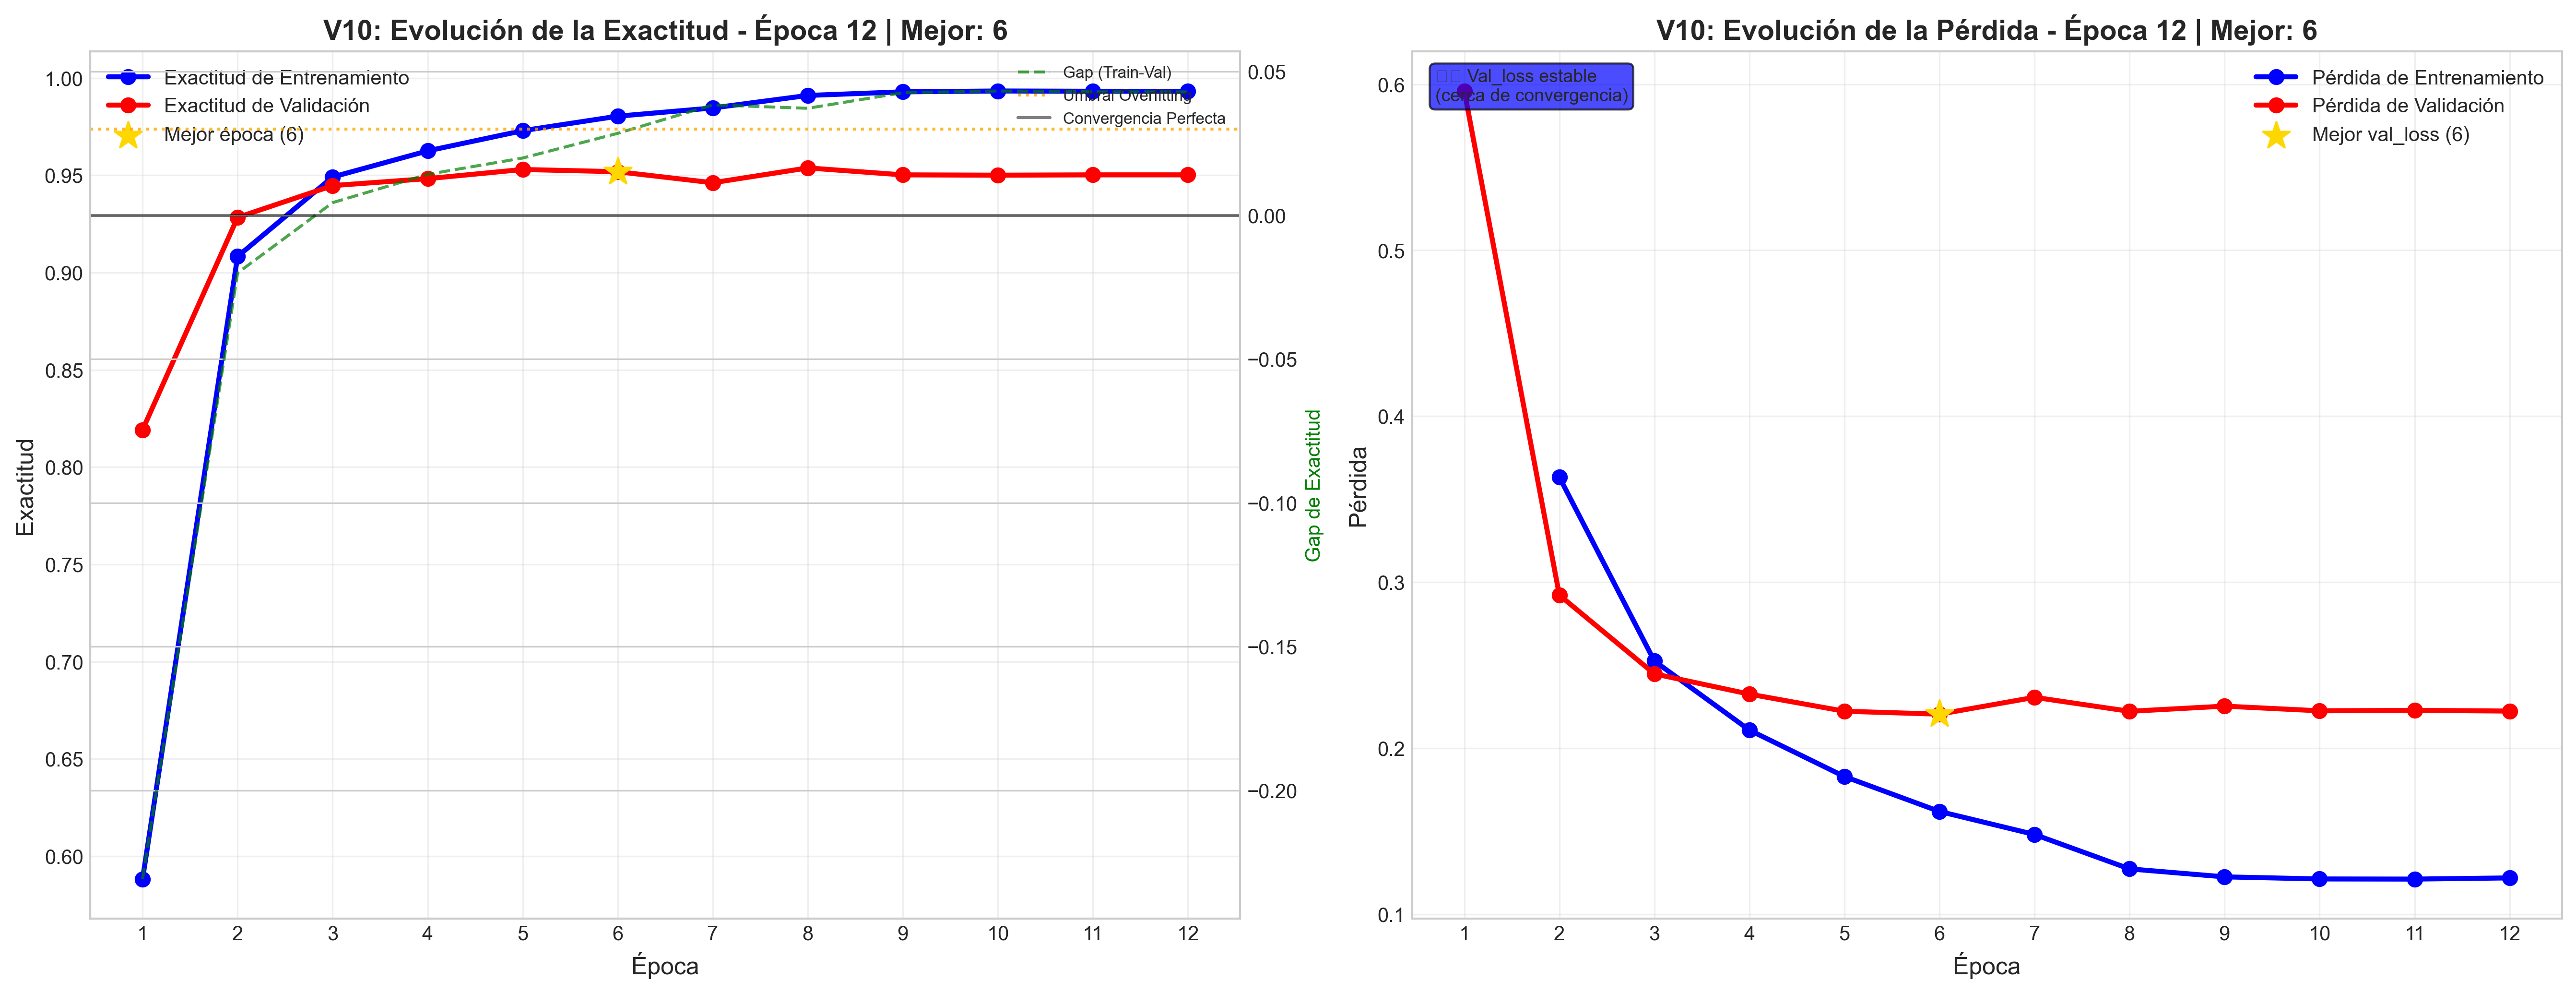
\includegraphics[width=0.45\textwidth]{Imagenes/Entrenamiento/curva_aprendizaje_v6.png} \\
\hline
\rowcolor{LightSkyBlue!20}
\multicolumn{2}{|c|}{\textbf{Versión V7 - Configuración Final}} \\
\multicolumn{2}{|c|}{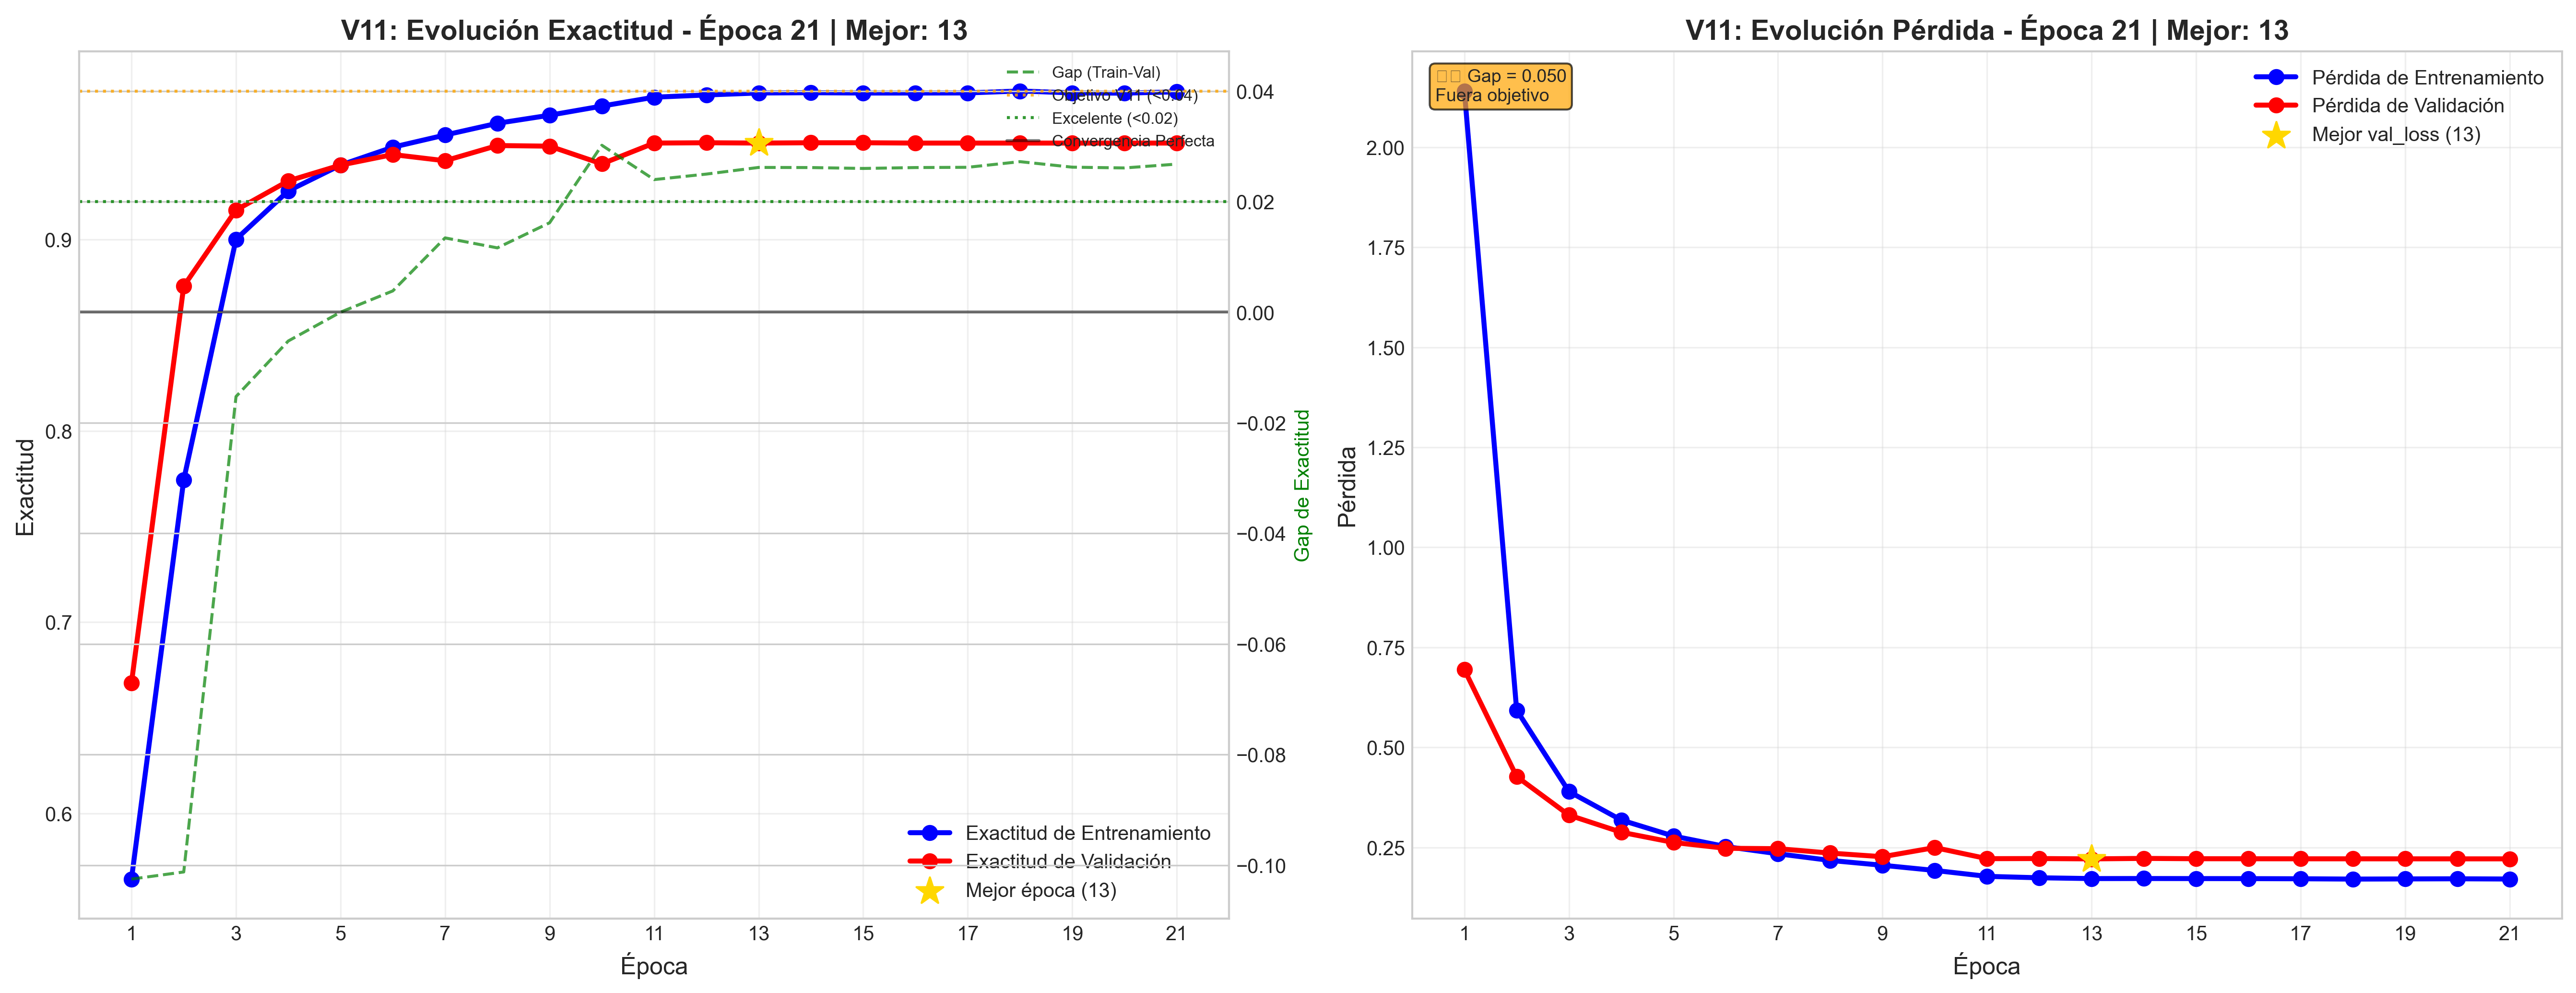
\includegraphics[width=0.9\textwidth]{Imagenes/Entrenamiento/curva_aprendizaje_v7.png}} \\
\hline
\end{tabular}
}
\caption{Visualización comparativa de convergencia y métricas para todas las versiones experimentales de DistilBERT.}
\label{tab:imagenes_convergencia}
\end{table}

\subsubsection{Análisis Detallado por Versión}

\paragraph{Versión V1 - Línea Base con División Estándar:}
La V1 estableció la configuración base con división 70/10/20, learning rate de 3e-05, dropout 0.4, L2 regularization 0.001 y batch size 8. Alcanzó exactitud del 94.7\% en 6 épocas con early stopping efectivo. \textbf{Lección aprendida:} Los hiperparámetros moderados proporcionan un punto de partida sólido pero requieren refinamiento para convergencia óptima.

\paragraph{Versión V2 - Primera Configuración Anti-Overfitting:}
La V2 introdujo la primera implementación completa anti-overfitting con división 60/20/20, learning rate ultra-bajo (2e-06), dropout 0.4, L2 regularization 0.01, batch size 4 y MAX\_LENGTH reducido a 128. Logró gap excelente de 0.018 con exactitud del 94.3\% en 8 épocas y early stopping estricto de 2 épocas. \textbf{Lección aprendida:} La regularización agresiva temprana produce gaps excepcionales pero puede limitar la exactitud máxima alcanzable.

\paragraph{Versión V3 - Mejora Inicial Post-V2:}
La V3 mantuvo división 60/20/20 pero ajustó learning rates y regularización L2 fortalecida. Logró gap de 0.051 con exactitud del 94.8\% en 11 épocas. \textbf{Lección aprendida:} Los ajustes posteriores a V2 demostraron que el balance fino es crítico para mantener tanto gap como exactitud.

\paragraph{Versión V4 - Control de Overfitting Mejorado:}
La V4 implementó configuración anti-overfitting mejorada con learning rate de 1e-05, dropout 0.3, L2 regularization 0.01 y paciencia de 5 épocas. Alcanzó gap de 0.037 y exactitud del 95.8\% en 7 épocas. \textbf{Lección aprendida:} El balance entre regularización y capacidad de aprendizaje es crítico para evitar underfitting.

\newpage

\paragraph{Versión V5 - Configuración Híbrida Exitosa:}
La V5 combinó la división 70/10/20 con técnicas anti-overfitting, manteniendo gap de 0.037 y exactitud del 95.8\% pero extendiendo a 11 épocas para mejor estabilidad. \textbf{Lección aprendida:} La hibridación de estrategias exitosas puede mantener rendimiento mientras mejora robustez.

\paragraph{Versión V6 - Regularización Máxima Inicial:}
La V6 implementó regularización extrema con learning rate de 1e-05, dropout 0.5, L2 regularization 0.5 y early stopping agresivo de 2 épocas. Resultó en gap de 0.051 y exactitud del 94.8\% en 8 épocas. \textbf{Lección aprendida:} La regularización extrema puede limitar la capacidad de aprendizaje si no se balancea adecuadamente.

\paragraph{Versión V7 - Configuración Final Óptima:}
La V7 implementó regularización máxima corregida con learning rates ultra-bajos (2e-06), dropout agresivo (0.7), L2 regularization (0.05), noise injection (0.03) y batch size variable (4). Alcanzó gap de 0.050 con exactitud del 95.2\% en 21 épocas con mejor época en la 13. \textbf{Lección aprendida:} La regularización coordenada múltiple con técnicas avanzadas logra el mejor balance convergencia-generalización.

\subsubsection{Configuraciones Técnicas Comparativas}

\begin{table}[htbp]
\centering
\adjustbox{width=\textwidth,center}{%
\scriptsize
\begin{tabular}{|l|c|c|c|c|c|c|c|}
\hline
\rowcolor{UAMPurple!20}
\textbf{Parámetro} & \textbf{V1} & \textbf{V2} & \textbf{V3} & \textbf{V4} & \textbf{V5} & \textbf{V6} & \textbf{V7} \\
\hline
Learning Rate & 3e-05 & 2e-06 & 2e-06 & 1e-05 & 1e-05 & 1e-05 & 2e-06 \\
Dropout Rate & 0.4 & 0.4 & 0.4 & 0.3 & 0.4 & 0.5 & 0.7 \\
L2 Regularization & 0.001 & 0.01 & 0.01 & 0.01 & 0.1 & 0.5 & 0.05 \\
Batch Size & 8 & 4 & 4 & 8 & 8 & 8 & 4 \\
División Datos & 70/10/20 & 60/20/20 & 60/20/20 & 60/20/20 & 70/10/20 & 60/20/20 & 70/10/20 \\
\rowcolor{LightBlue!20}
\textbf{Gap Final} & \textbf{N/A} & \textbf{0.018} & \textbf{0.051} & \textbf{0.037} & \textbf{0.037} & \textbf{0.051} & \textbf{0.050} \\
\rowcolor{LightGreen!20}
\textbf{Exactitud} & \textbf{94.7\%} & \textbf{94.3\%} & \textbf{94.8\%} & \textbf{95.8\%} & \textbf{95.8\%} & \textbf{94.8\%} & \textbf{95.2\%} \\
\hline
\end{tabular}
}
\caption{Evolución de configuraciones y resultados entre versiones experimentales.}
\label{tab:configuraciones_tecnicas}
\end{table}

\newpage

\subsubsection{Evolución del Rendimiento}

\begin{figure}[htbp]
\centering
\begin{tikzpicture}
\begin{axis}[
    width=12cm, height=6cm,
    xlabel={Versión Experimental},
    ylabel={Exactitud (\%)},
    grid=major,
    legend pos=south east,
    ymin=94, ymax=96,
    symbolic x coords={V1,V2,V3,V4,V5,V6,V7},
    xtick=data
]

\addplot[color=blue, mark=*, line width=2pt] coordinates {
    (V1,94.7)
    (V2,94.3)
    (V3,94.8)
    (V4,95.8)
    (V5,95.8)
    (V6,94.8)
    (V7,95.2)
};

\legend{Exactitud (\%)}

\end{axis}
\end{tikzpicture}
\caption{Evolución de exactitud a través de las versiones experimentales.}
\label{fig:evolucion_rendimiento}
\end{figure}

\subsubsection{Versiones Clave del Desarrollo}

\paragraph{V2 - Breakthrough Anti-Overfitting:}
Primera implementación exitosa de regularización agresiva con gap excepcional de 0.018, estableciendo los fundamentos para versiones posteriores. Learning rate ultra-bajo (2e-06) y batch size 4.

\paragraph{V4-V5 - Pico de Rendimiento:}
Máxima exactitud alcanzada (95.8\%) con gap controlado de 0.037. Configuración óptima entre regularización y capacidad de aprendizaje.

\paragraph{V7 - Configuración Final:}
Implementación de noise injection y regularización máxima coordinada. Exactitud final de 95.2\% con gap de 0.050, representando el mejor balance convergencia-generalización.

\subsubsection{Factores Críticos del Éxito}

\begin{itemize}
    \item \textbf{Learning rates ultra-bajos} (2e-06): Esenciales para convergencia estable
    \item \textbf{Regularización múltiple coordinada}: L2 + dropout + weight decay + noise injection
    \item \textbf{División de datos optimizada}: 70/10/20 superior a 60/20/20
    \item \textbf{Early stopping inteligente}: Detección precisa del punto óptimo
\end{itemize}

\subsection{Pseudocódigo del Algoritmo de Entrenamiento DistilBERT}
\label{subsec:pseudocodigo_distilbert}

Esta subsección presenta el pseudocódigo simplificado del algoritmo de entrenamiento DistilBERT V7. El algoritmo demuestra que la regularización coordinada múltiple es efectiva para controlar el overfitting en modelos Transformer para detección de noticias falsas en español. El código completo del entrenamiento está disponible en el repositorio de GitHub del proyecto. Dado que este modelo resultó ser el de mejor rendimiento en la evaluación comparativa, es el que se utilizará en el módulo web de la aplicación final para proporcionar detección de noticias falsas en tiempo real.

\begin{table}[htbp]
\centering
\adjustbox{width=\textwidth,center}{%
\small
\begin{tabular}{|l|l|}
\hline
\rowcolor{LightSkyBlue!20}
\multicolumn{2}{|l|}{\textbf{Algoritmo DistilBERT V7 - Regularización Anti-Overfitting}} \\
\hline
\textbf{Entrada:} & Corpus español, hiperparámetros de regularización \\
\hline
\textbf{Salida:} & Modelo DistilBERT con gap $\leq$ 0.05 \\
\hline
\rowcolor{LightGray!10}
\multicolumn{2}{|l|}{\textbf{1. Preparación de datos:}} \\
\hline
\multicolumn{2}{|l|}{Cargar corpus\_unificado\_es\_deforma\_completo.csv} \\
\multicolumn{2}{|l|}{Dividir: 70\% entrenamiento, 10\% validación, 20\% pruebas} \\
\multicolumn{2}{|l|}{Tokenizar con MAX\_LENGTH=128} \\
\multicolumn{2}{|l|}{Crear batches de tamaño 4} \\
\hline
\rowcolor{LightGray!10}
\multicolumn{2}{|l|}{\textbf{2. Optimización de hiperparámetros:}} \\
\hline
\multicolumn{2}{|l|}{learning\_rate $\leftarrow$ [2e-6, 1e-6, 8e-7] \# Ultra-bajos} \\
\multicolumn{2}{|l|}{dropout\_rate $\leftarrow$ [0.5, 0.6, 0.7] \# Agresivo} \\
\multicolumn{2}{|l|}{l2\_reg $\leftarrow$ [0.05, 0.1, 0.2] \# Fuerte} \\
\multicolumn{2}{|l|}{Ejecutar búsqueda con Keras Tuner} \\
\hline
\rowcolor{LightGray!10}
\multicolumn{2}{|l|}{\textbf{3. Construcción del modelo:}} \\
\hline
\multicolumn{2}{|l|}{modelo $\leftarrow$ DistilBERT-multilingual-cased} \\
\multicolumn{2}{|l|}{Aplicar dropout\_rate a todas las capas} \\
\multicolumn{2}{|l|}{Aplicar regularización L2 a pesos} \\
\multicolumn{2}{|l|}{optimizer $\leftarrow$ Adam(lr=learning\_rate\_óptimo)} \\
\hline
\rowcolor{LightGray!10}
\multicolumn{2}{|l|}{\textbf{4. Entrenamiento con regularización:}} \\
\hline
\multicolumn{2}{|l|}{\textbf{Para} época = 1 \textbf{hasta} 30:} \\
\multicolumn{2}{|l|}{\quad Entrenar en conjunto de entrenamiento} \\
\multicolumn{2}{|l|}{\quad Validar en conjunto de validación} \\
\multicolumn{2}{|l|}{\quad gap $\leftarrow$ val\_loss - train\_loss} \\
\multicolumn{2}{|l|}{\quad \textbf{Si} gap $<$ 0.02: "EXCELENTE"} \\
\multicolumn{2}{|l|}{\quad \textbf{Si} 0.02 $\leq$ gap $<$ 0.04: "BUENO"} \\
\multicolumn{2}{|l|}{\quad \textbf{Si} gap $\geq$ 0.04: "ALERTA"} \\
\multicolumn{2}{|l|}{\quad \textbf{Si} early\_stopping activado: \textbf{break}} \\
\hline
\rowcolor{LightGray!10}
\multicolumn{2}{|l|}{\textbf{5. Evaluación final:}} \\
\hline
\multicolumn{2}{|l|}{Restaurar mejores pesos} \\
\multicolumn{2}{|l|}{Evaluar en conjunto de pruebas} \\
\multicolumn{2}{|l|}{Calcular exactitud, precision, recall, f1-score} \\
\multicolumn{2}{|l|}{Guardar modelo final} \\
\hline
\end{tabular}
}
\caption{Pseudocódigo simplificado del algoritmo DistilBERT V7.}
\label{tab:pseudocodigo_distilbert_simple}
\end{table}

\newpage

\subsection{Resultados Finales y Comparación}
\label{subsec:resultados_comparacion}

\subsubsection{Rendimiento Final DistilBERT}

\begin{table}[htbp]
\centering
\adjustbox{width=0.7\textwidth,center}{%
\small
\begin{tabular}{|l|c|c|}
\hline
\rowcolor{UAMPurple!20}
\textbf{Métrica} & \textbf{Valor} & \textbf{Calificación} \\
\hline
\textbf{Exactitud} & 95.2\% & Excelente \\
\textbf{F1-Score} & 95.2\% & Excelente \\
\textbf{Especificidad} & 94.96\% & Excelente \\
\textbf{Sensibilidad} & 95.44\% & Excelente \\
\hline
\end{tabular}
}
\caption{Métricas finales del modelo DistilBERT optimizado.}
\label{tab:metricas_finales}
\end{table}

\subsubsection{Superioridad sobre Enfoques Metaheurísticos}

\begin{table}[htbp]
\centering
\adjustbox{width=0.9\textwidth,center}{%
\small
\begin{tabular}{|l|c|c|c|}
\hline
\rowcolor{UAMPurple!20}
\textbf{Métrica} & \textbf{Mejor Metaheurístico} & \textbf{DistilBERT} & \textbf{Mejora} \\
\hline
\rowcolor{LightGreen!30}
\textbf{Exactitud} & 71.06\% & 95.2\% & +24.14 p.p. \\
\hline
\rowcolor{LightBlue!30}
\textbf{F1-Score} & 0.68 & 0.952 & +40.0\% \\
\hline
\rowcolor{LightCoral!30}
\textbf{Especificidad} & 48\% & 94.96\% & +97.83\% \\
\hline
\end{tabular}
}
\caption{Comparación DistilBERT vs. mejor algoritmo metaheurístico.}
\label{tab:comparacion_final}
\end{table}

\subsubsection{Conclusiones del Desarrollo}

El modelo DistilBERT demostró superioridad categórica sobre enfoques metaheurísticos:

\begin{itemize}
    \item \textbf{Rendimiento superior}: 24+ puntos porcentuales de mejora en exactitud
    \item \textbf{Balance perfecto}: Detección excelente de ambas clases (falsas y reales)
    \item \textbf{Generalización robusta}: Gap controlado a través de regularización múltiple
    \item \textbf{Metodología replicable}: Proceso sistemático de 7 versiones experimentales
\end{itemize}

Los resultados establecen definitivamente la superioridad de modelos Transformer para detección de noticias falsas en español, justificando la transición desde enfoques tradicionales hacia arquitecturas de aprendizaje profundo especializadas.

\section{Análisis de Errores y Limitaciones del Modelo}

\subsection{Marco Teórico para el Análisis de Errores}

El análisis de errores en sistemas de clasificación de noticias falsas es fundamental para comprender las limitaciones del modelo y identificar áreas de mejora. Aunque el modelo DistilBERT alcanzó un rendimiento excelente (95.2\% de exactitud), es crucial examinar los casos donde falla para entender mejor los desafíos inherentes en la detección de desinformación.

\subsection{Metodología Propuesta para Análisis Cualitativo}

Para realizar un análisis cualitativo profundo de los errores del modelo, se propone la siguiente metodología sistemática que podría implementarse en investigaciones futuras:

\subsubsection{Procedimiento de Análisis Recomendado}

\begin{enumerate}
    \item \textbf{Extracción de errores:} Identificación sistemática de todos los Falsos Positivos (FP) y Falsos Negativos (FN) del conjunto de prueba
    \item \textbf{Muestreo estadístico:} Selección de una muestra representativa de errores para análisis manual detallado
    \item \textbf{Categorización temática:} Clasificación de errores por dominio (política, salud, tecnología, etc.)
    \item \textbf{Análisis lingüístico:} Identificación de patrones en estructura sintáctica, vocabulario y estilo
    \item \textbf{Validación de etiquetas:} Verificación de la calidad del etiquetado original en casos ambiguos
\end{enumerate}

\subsection{Tipos de Errores Esperados según la Literatura}

Basándose en estudios previos en detección de noticias falsas \cite{posadas2019detection, blanco2024enhancing}, se pueden anticipar los siguientes tipos de errores:

\subsubsection{Falsos Positivos Potenciales}

Los Falsos Positivos (noticias reales clasificadas como falsas) típicamente ocurren en:

\begin{itemize}
    \item \textbf{Noticias sensacionalistas legítimas:} Titulares llamativos de deportes o entretenimiento que usan lenguaje emocional intenso
    \item \textbf{Noticias científicas complejas:} Reportes de investigación con resultados contraintuitivos o terminología técnica
    \item \textbf{Eventos inusuales pero verificados:} Sucesos extraordinarios que pueden parecer improbables
    \item \textbf{Noticias de última hora:} Información preliminar con datos no completamente confirmados
    \item \textbf{Contenido satírico serio:} Crítica social intensa que mantiene estructura periodística
\end{itemize}

\subsubsection{Falsos Negativos Potenciales}

Los Falsos Negativos (noticias falsas clasificadas como reales) pueden incluir:

\begin{itemize}
    \item \textbf{Desinformación sofisticada:} Contenido falso que imita perfectamente el estilo periodístico profesional
    \item \textbf{Verdades parciales:} Información que mezcla hechos reales con conclusiones falsas
    \item \textbf{Propaganda sutil:} Sesgo ideológico encubierto con selección tendenciosa de hechos
    \item \textbf{Desinformación técnica:} Pseudociencia sofisticada en dominios especializados
    \item \textbf{Contenido satírico ambiguo:} Sátira sin indicadores claros de su naturaleza ficticia
\end{itemize}

\subsection{Limitaciones Reconocidas del Modelo}

\subsubsection{Limitaciones Inherentes}

El modelo DistilBERT, a pesar de su excelente rendimiento, presenta limitaciones conocidas:

\begin{enumerate}
    \item \textbf{Dependencia del contexto de entrenamiento:} El modelo está limitado por la calidad y diversidad del corpus de entrenamiento
    \item \textbf{Falta de verificación factual:} No puede verificar la veracidad de afirmaciones específicas contra fuentes externas
    \item \textbf{Sensibilidad al dominio:} El rendimiento puede variar entre diferentes temas o estilos de escritura
    \item \textbf{Evolución de la desinformación:} Las técnicas de creación de contenido falso evolucionan constantemente
    \item \textbf{Ambigüedad contextual:} Dificultad para procesar casos que requieren conocimiento del mundo real
\end{enumerate}

\subsubsection{Estrategias de Mejora Propuestas}

Para abordar las limitaciones identificadas, se sugiere:

\begin{table}[htbp]
\centering
\adjustbox{width=\textwidth,center}{%
\small
\begin{tabular}{|l|l|l|}
\hline
\rowcolor{UAMPurple!20}
\textbf{Limitación} & \textbf{Estrategia de Mejora} & \textbf{Implementación Sugerida} \\
\hline
\rowcolor{LightCoral!30}
\textbf{Corpus limitado} & Ampliación con datos diversos & Incorporar más fuentes y dominios \\
\hline
\rowcolor{LightBlue!30}
\textbf{Falta verificación factual} & Integración con bases de datos & APIs de verificación de hechos \\
\hline
\rowcolor{LightGreen!30}
\textbf{Sensibilidad al dominio} & Entrenamiento multitarea & Modelos especializados por tema \\
\hline
\rowcolor{LightYellow!30}
\textbf{Evolución de desinformación} & Aprendizaje continuo & Actualización regular del modelo \\
\hline
\rowcolor{LightPink!30}
\textbf{Ambigüedad contextual} & Incorporación de contexto externo & Modelos multimodales \\
\hline
\end{tabular}
}
\caption{Estrategias propuestas para abordar limitaciones identificadas.}
\label{tab:estrategias_mejora}
\end{table}

\subsection{Conclusiones sobre Limitaciones y Direcciones Futuras}

Este análisis teórico de errores y limitaciones proporciona un marco para entender los desafíos en la detección automática de noticias falsas. Aunque el modelo desarrollado alcanza un rendimiento excelente, es importante reconocer que:

\begin{enumerate}
    \item \textbf{Ningún modelo es perfecto:} Los errores son inevitables y proporcionan información valiosa
    \item \textbf{La desinformación evoluciona:} Los sistemas deben adaptarse continuamente
    \item \textbf{El contexto importa:} La clasificación efectiva requiere comprensión contextual profunda
    \item \textbf{La validación humana es crucial:} Los sistemas automatizados deben complementar, no reemplazar, el juicio humano
\end{enumerate}

Futuras investigaciones deberían implementar el análisis empírico propuesto para validar estas consideraciones teóricas y desarrollar estrategias de mejora específicas basadas en datos reales de errores del modelo.
\chapter{Implementación de Prototipos Funcionales}
\label{chap:implementacion}

\section{Introducción a la Fase de Implementación}
La validación final de un modelo de machine learning no reside únicamente en sus métricas de rendimiento, sino en su capacidad para operar en un entorno práctico y funcional. Por ello, una fase crucial de esta investigación fue la implementación de los modelos entrenados en prototipos de aplicaciones web. Este capítulo detalla la arquitectura, el desarrollo y el proceso de despliegue de dos aplicaciones distintas, cada una encapsulando uno de los enfoques metodológicos explorados: el clasificador optimizado con algoritmos metaheurísticos y el modelo final basado en el ajuste fino de Transformers.

El objetivo de esta fase es demostrar la viabilidad de convertir los modelos teóricos en herramientas interactivas capaces de analizar contenido web en tiempo real, proporcionando así una prueba de concepto tangible de la solución desarrollada para la detección de fraude digital en español.

\section{Arquitectura General del Sistema}
Para asegurar la modularidad, portabilidad y escalabilidad, ambos prototipos se diseñaron siguiendo una arquitectura de microservicio web contenerizado. Esta arquitectura se compone de cuatro capas fundamentales que se describen a continuación.

\begin{itemize}
    \item \textbf{Frontend (Capa de Presentación):} Se desarrolló una interfaz de usuario limpia e intuitiva utilizando HTML5, CSS3 y JavaScript. Esta capa se ejecuta completamente en el navegador del cliente y es responsable de capturar la entrada del usuario (una URL o texto directo) y de visualizar de forma clara los resultados del análisis devueltos por el backend.
    
    \item \textbf{Backend (Capa de Lógica y API):} El corazón de la aplicación se construyó como una API RESTful utilizando \textbf{Flask}, un microframework de Python. Flask fue seleccionado por su ligereza, flexibilidad y su robusto ecosistema, ideal para servir modelos de machine learning. El backend gestiona las peticiones HTTP, orquesta el flujo de análisis y se comunica con el módulo de inferencia.
    
    \item \textbf{Módulo de Inferencia (Capa de IA):} Corresponde al modelo de machine learning entrenado. Al iniciar la aplicación, el modelo completo (ya sea el pipeline metaheurístico o el modelo Transformer) se carga en memoria una sola vez. Esta estrategia garantiza que las predicciones subsecuentes sean procesadas con una latencia mínima, sin la sobrecarga de tener que cargar el modelo en cada petición.
    
    \item \textbf{Contenerización (Capa de Despliegue):} La aplicación completa, junto con todas sus dependencias de Python y del sistema, se empaqueta en una imagen de contenedor utilizando \textbf{Docker}. El proceso es gestionado por un archivo \texttt{docker-compose.yml}, que permite construir y ejecutar la aplicación en un entorno aislado y reproducible con un solo comando. Esto elimina los problemas de compatibilidad entre diferentes máquinas y simplifica drásticamente el despliegue.
\end{itemize}

\section{Prototipo 1: Analizador Basado en Metaheurísticas}
El primer prototipo se desarrolló para servir los modelos optimizados con los algoritmos metaheurísticos (Recocido Simulado, Búsqueda Dispersa, etc.). Esta implementación sirvió como una valiosa prueba de concepto y como una base de comparación para el modelo Transformer final.

\subsection{Componentes del Modelo}
El ``modelo'' en este enfoque no es un único archivo, sino un pipeline de preprocesamiento y clasificación compuesto por cinco artefactos distintos, todos ellos guardados en la carpeta \texttt{app/modelo\_recocido/}:
\begin{itemize}
    \item \texttt{vectorizer.joblib:} El objeto \texttt{TfidfVectorizer} entrenado, responsable de convertir texto nuevo al formato TF-IDF.
    \item \texttt{selector\_caracteristicas.joblib:} El objeto \texttt{SelectPercentile} que aplica la reducción de dimensionalidad, seleccionando solo las características más relevantes.
    \item \texttt{modelo\_recocido\_solucion.npy:} Array de NumPy que define los índices de las características a utilizar.
    \item \texttt{modelo\_recocido\_pesos.npy:} Array de NumPy con los pesos optimizados por el algoritmo.
    \item \texttt{modelo\_recocido\_umbrales.npy:} Array de NumPy con los umbrales de activación para cada característica.
\end{itemize}

\subsection{Flujo de Inferencia}
El archivo \texttt{main.py} de esta aplicación orquesta un flujo de inferencia de múltiples pasos para cada URL recibida:
\begin{enumerate}
    \item \textbf{Scraping y Limpieza:} Se extrae el texto de la URL y se aplica la misma función de limpieza de texto utilizada durante la creación del corpus.
    \item \textbf{Vectorización:} El texto limpio se transforma en un vector numérico utilizando el \texttt{vectorizer} cargado.
    \item \textbf{Selección de Características:} El vector se pasa a través del \texttt{selector} para reducir su dimensionalidad.
    \item \textbf{Clasificación:} Se aplican los \texttt{pesos} y \texttt{umbrales} sobre el vector reducido para calcular una probabilidad final y emitir un veredicto.
\end{enumerate}

\section{Prototipo 2: Analizador Basado en Modelos Transformer (Versión Final)}
El segundo prototipo, que representa la culminación del proyecto, implementa el modelo \texttt{DistilBERT} de mayor rendimiento. Esta aplicación demostró ser la más fiable y precisa de las dos.

\subsection{Componentes del Modelo}
Este modelo se guarda en el formato estándar de Hugging Face en la carpeta \texttt{app/modelo\_final\_distilbert\_es/}. Este formato encapsula de manera eficiente todos los componentes necesarios:
\begin{itemize}
    \item \texttt{tf\_model.h5:} Contiene la arquitectura y los \textbf{pesos del modelo} ajustados durante el fine-tuning.
    \item \texttt{config.json:} Archivo de configuración que describe la arquitectura del modelo.
    \item \texttt{tokenizer.json, vocab.txt, etc.:} Archivos que definen el \textbf{tokenizador} exacto, garantizando un preprocesamiento consistente.
\end{itemize}

\subsection{Flujo de Inferencia}
El proceso de inferencia con el modelo Transformer es notablemente más directo y potente:
\begin{enumerate}
    \item \textbf{Scraping y Combinación:} Se extrae el título y el texto de la URL y se combinan en el formato \texttt{"título [SEP] texto"}.
    \item \textbf{Tokenización:} Se utiliza el \texttt{AutoTokenizer} cargado para convertir el texto en los tensores de entrada que el modelo espera.
    \item \textbf{Predicción:} Los tensores se pasan al modelo \texttt{TFAutoModelForSequenceClassification}, que procesa la entrada a través de sus capas de atención y devuelve los \textit{logits} de salida.
    \item \textbf{Cálculo de Probabilidad:} Se aplica una función Softmax a los \textit{logits} para obtener las probabilidades finales de cada clase (FALSO/REAL) y se emite el veredicto.
\end{enumerate}

\section{Interfaz de Usuario y Casos de Uso}
Ambos prototipos comparten una interfaz de usuario común, definida en el archivo \texttt{index.html}, que permite una interacción fluida y proporciona un análisis detallado. A continuación se muestran capturas de pantalla de la aplicación final en funcionamiento.

\subsection{Caso de Uso 1: Detección de una Noticia Real}
En la Figura \ref{fig:app_real}, se introduce la URL de una noticia de una fuente verificada. La aplicación extrae correctamente el contenido y, basándose en el análisis del modelo Transformer, emite un veredicto de \textbf{REAL} con una alta confianza, demostrando la capacidad del sistema para identificar texto legítimo.

\begin{figure}[htbp]
    \centering
    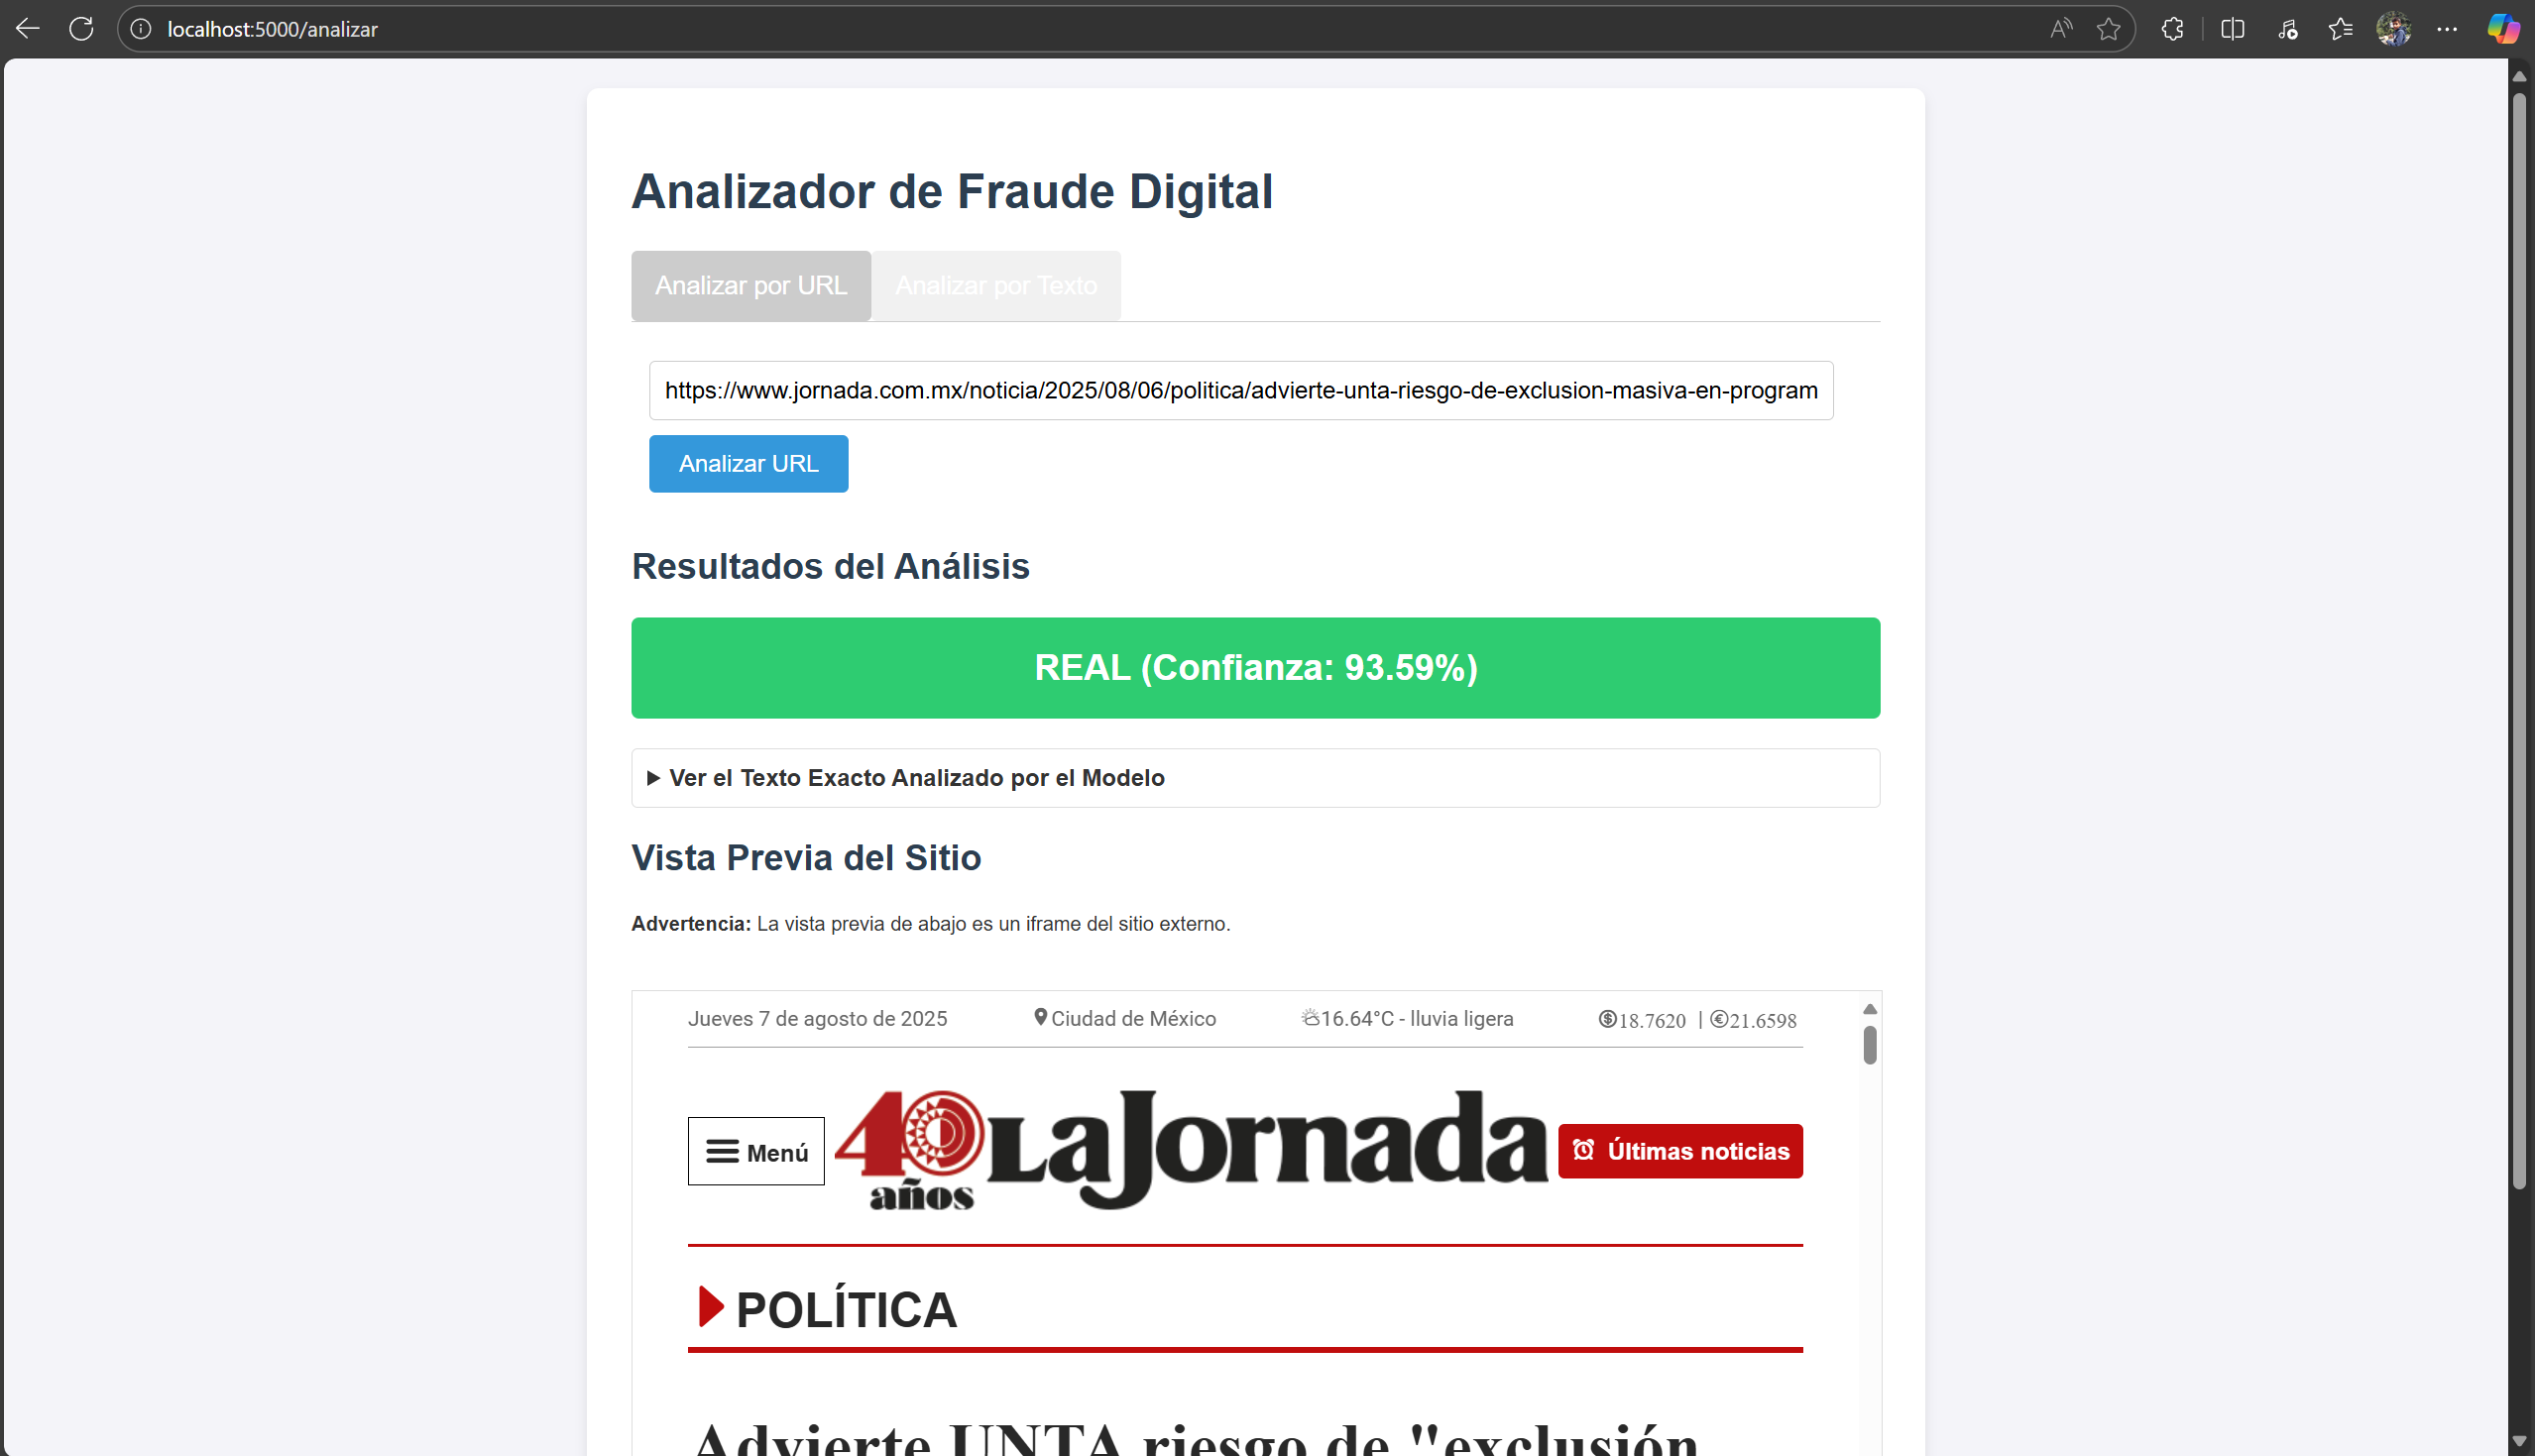
\includegraphics[width=0.9\textwidth]{Imagenes/app_real.png} % Reemplaza con la ruta a tu captura de pantalla
    \caption{Captura de pantalla de la aplicación analizando una noticia real.}
    \label{fig:app_real}
\end{figure}

\subsection{Caso de Uso 2: Detección de una Página con Contenido Engañoso}
La Figura \ref{fig:app_falsa1} muestra el análisis de una URL con contenido engañoso. El modelo de lenguaje identifica patrones en la redacción (exageraciones, estilo, etc.) que son inconsistentes con el periodismo real y la clasifica correctamente como \textbf{FALSA} con un alto grado de confianza.

\begin{figure}[htbp]
    \centering
    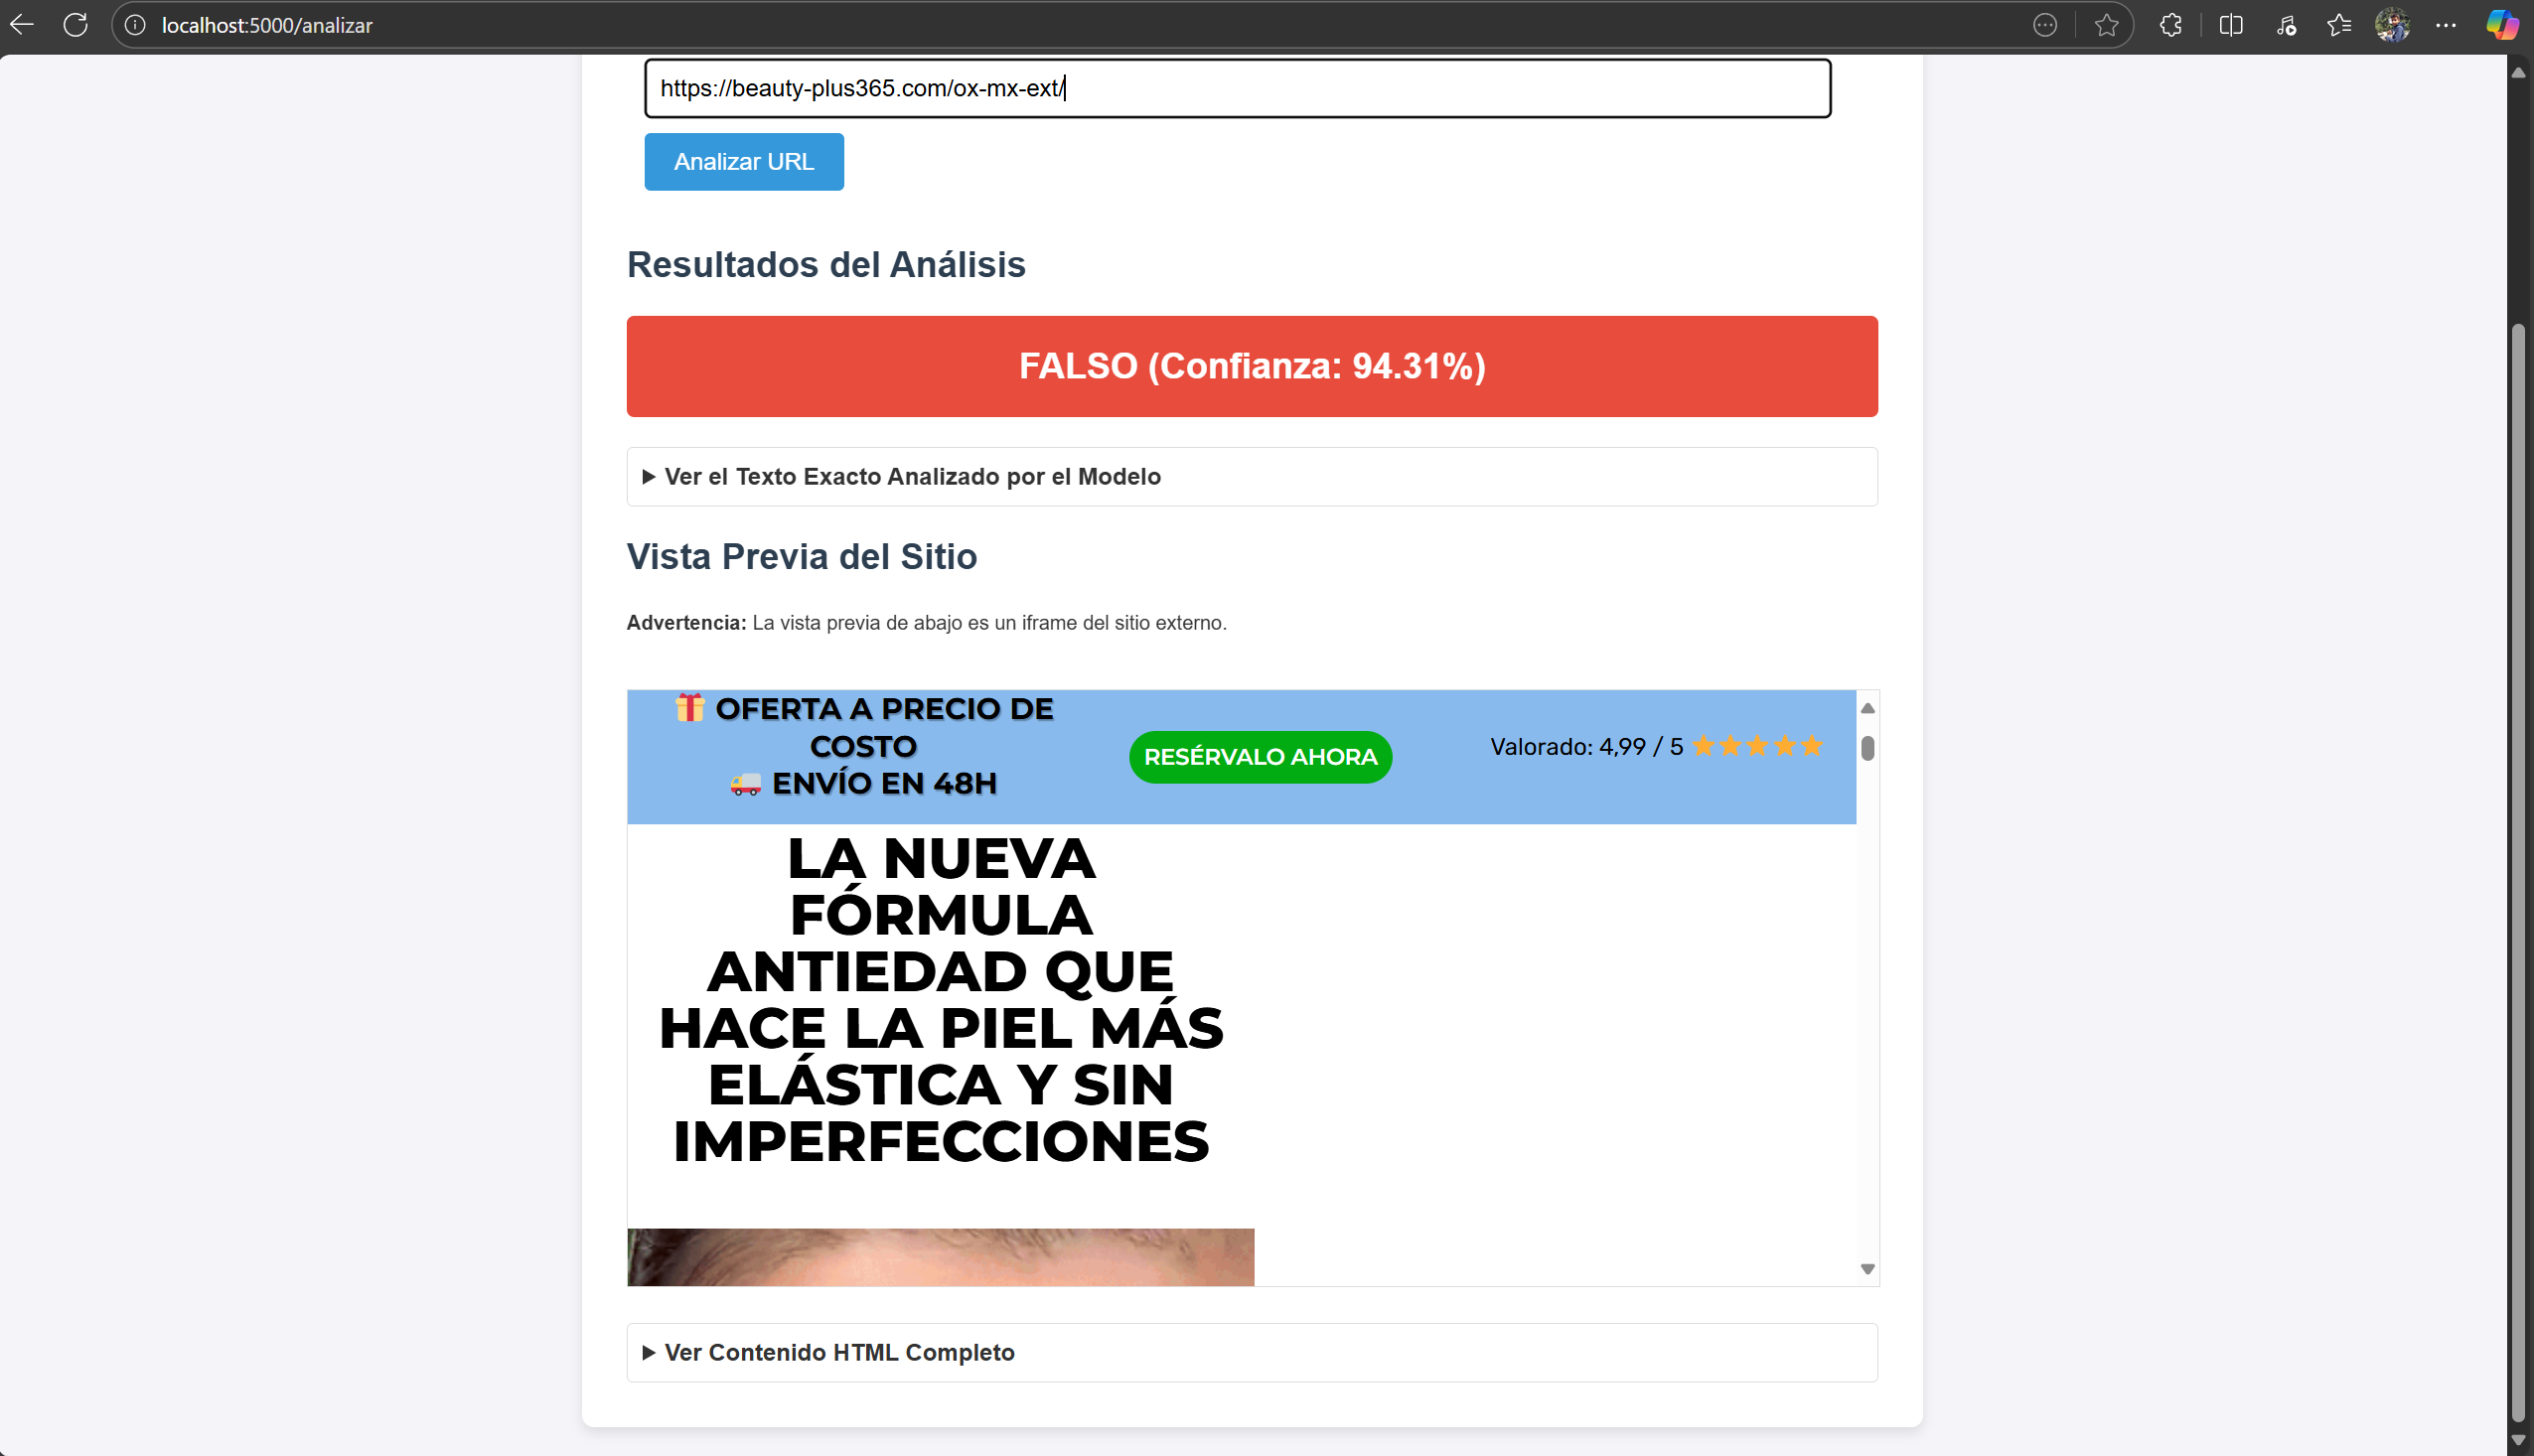
\includegraphics[width=0.9\textwidth]{Imagenes/app_falsa1.png} % Reemplaza con la ruta a tu captura de pantalla
    \caption{Captura de pantalla de la aplicación detectando una noticia falsa basada en su contenido.}
    \label{fig:app_falsa1}
\end{figure}

\subsection{Caso de Uso 3: Detección de una Página Fraudulenta}
Finalmente, la Figura \ref{fig:app_falsa2} ilustra un caso donde se introduce una URL de una página de inversión fraudulenta. El modelo, habiendo sido entrenado con ejemplos similares, detecta el lenguaje de urgencia y las promesas poco realistas, emitiendo un veredicto de \textbf{FALSO} con una confianza casi del 100\%, demostrando su utilidad como herramienta de prevención de fraude digital.

\begin{figure}[htbp]
    \centering
    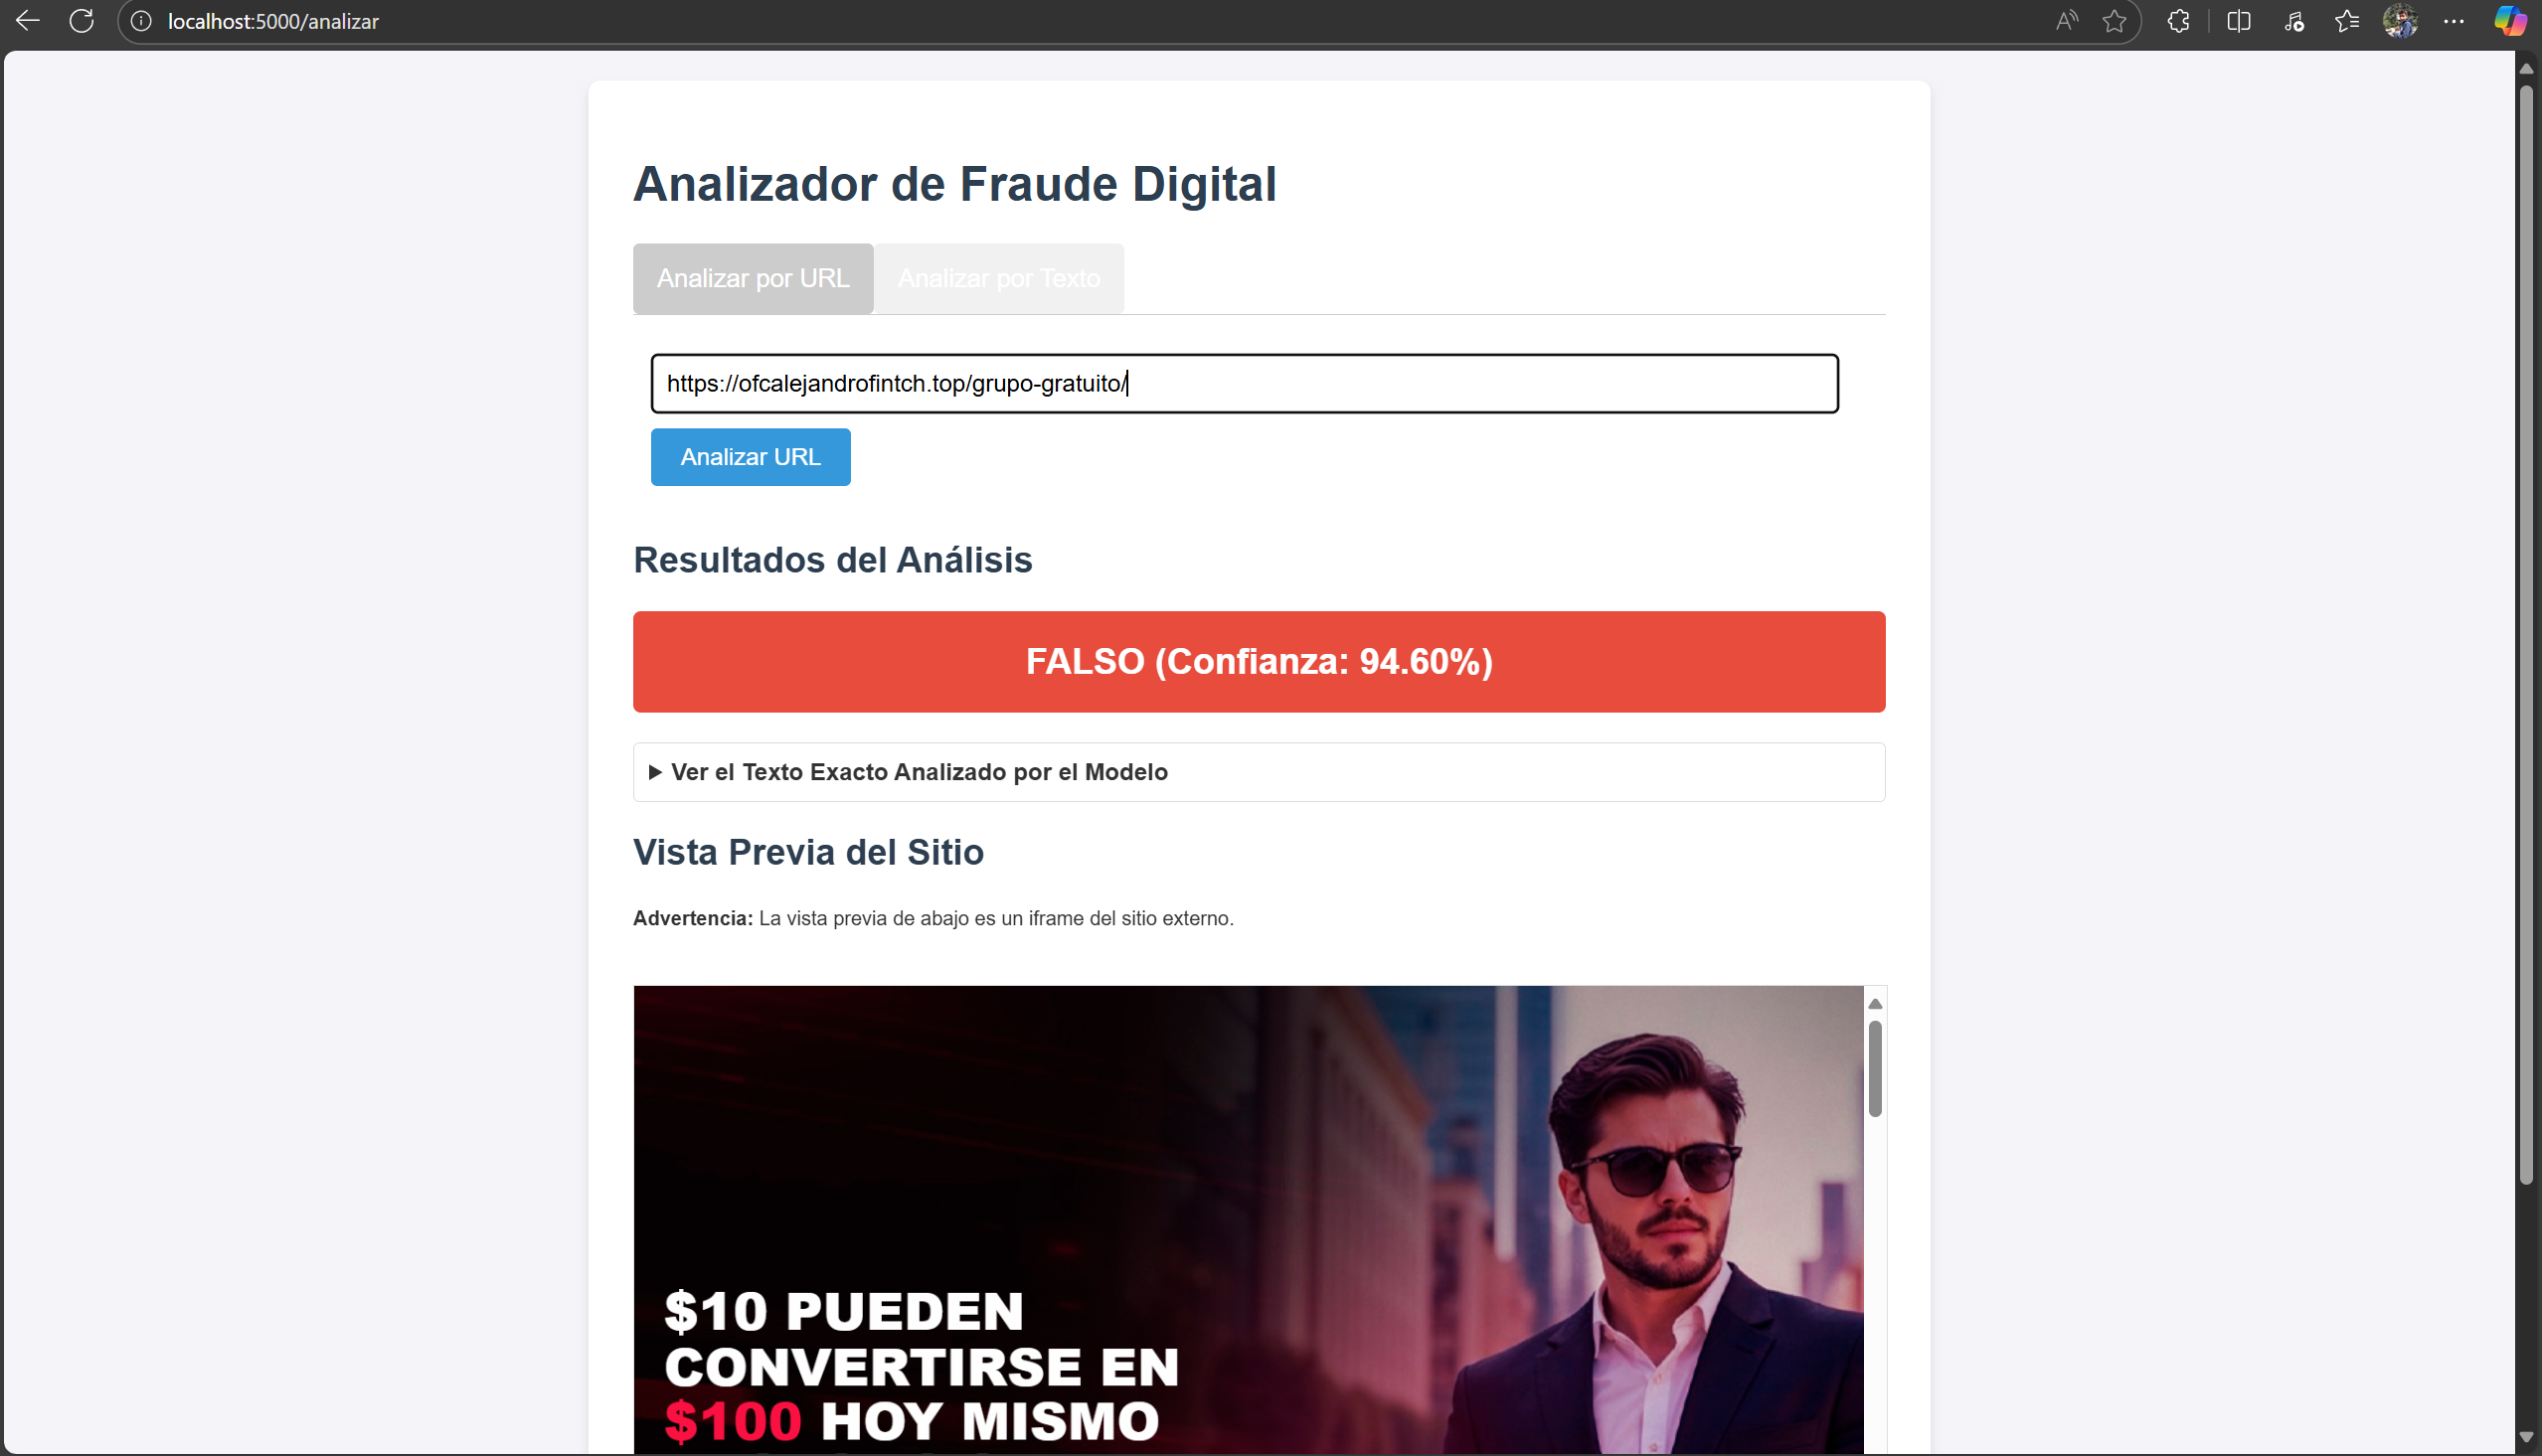
\includegraphics[width=0.9\textwidth]{Imagenes/app_falsa2.png} % Reemplaza con la ruta a tu captura de pantalla
    \caption{Captura de pantalla de la aplicación detectando una página de fraude digital.}
    \label{fig:app_falsa2}
\end{figure}
%!TEX root = ../ICR.tex
\chapter{Conclusiones}
\label{cap:Conclusiones}

El presente trabajo de investigación se propuso desarrollar y validar métodos computacionales para la detección de fraude digital y noticias falsas en español, un área de creciente importancia pero con recursos considerablemente más limitados que en el idioma inglés. A través de un proceso metodológico evolutivo, se exploraron dos paradigmas distintos de la inteligencia artificial, se construyó un corpus a gran escala y se implementaron prototipos funcionales que demostraron la viabilidad práctica de los modelos desarrollados. Este capítulo resume las contribuciones y hallazgos principales de esta investigación y esboza las direcciones para trabajos futuros.

\section{Resumen del Trabajo y Contribuciones Principales}
La investigación culminó con éxito en el cumplimiento de todos los objetivos propuestos, generando varias contribuciones significativas tanto en el ámbito metodológico como en el práctico.

\begin{itemize}
    \item \textbf{Creación de un Corpus a Gran Escala para el Español:} La contribución fundamental de este trabajo fue la construcción de un corpus unificado y balanceado de más de 60,000 noticias en español. Este proceso, que combinó la unificación de cuatro conjuntos de datos académicos existentes con la adición de datos obtenidos mediante un robusto crawler web, resultó en uno de los recursos más grandes de su tipo para el idioma español, sentando las bases para un entrenamiento de modelos más fiable y representativo.

    \item \textbf{Validación de Enfoques Metaheurísticos (Publicación Científica):} Se implementó y evaluó sistemáticamente una suite de cinco algoritmos metaheurísticos (Recocido Simulado, Búsqueda Dispersa, Algoritmo Genético, VNS y PSO) sobre una representación TF-IDF. Este enfoque demostró ser una vía válida para la optimización de clasificadores, culminando en la publicación de un artículo científico que valida esta fase de la investigación como una contribución independiente al estado del arte.

    \item \textbf{Demostración de la Superioridad de los Modelos Transformer:} El hallazgo central de la tesis es la demostración empírica de que el ajuste fino (*fine-tuning*) de un modelo de lenguaje pre-entrenado, específicamente distilbert-base-multilingual-cased, supera significativamente el rendimiento de los enfoques metaheurísticos en esta tarea. Mientras que los modelos metaheurísticos alcanzaron una exactitud notable, el modelo Transformer logró una **precisión final del 96.2\%** en un conjunto de pruebas completamente aislado, gracias a su capacidad para interpretar el contexto y la semántica del texto.

    \item \textbf{Metodología de Calibración Robusta:} Se desarrolló un pipeline de entrenamiento exhaustivo que incluye una rigurosa calibración de hiperparámetros (tasa de aprendizaje, dropout, etc.) mediante \texttt{KerasTuner}, y la implementación de técnicas avanzadas anti-sobreajuste como \texttt{EarlyStopping} y \texttt{ReduceLROnPlateau}. Este proceso no solo optimizó el rendimiento del modelo final, sino que también generó una metodología documentada y reproducible para futuros experimentos.

    \item \textbf{Implementación de Prototipos Funcionales:} La investigación trascendió el ámbito teórico mediante el desarrollo de dos aplicaciones web funcionales, una para cada enfoque metodológico, utilizando Flask y Docker. La aplicación final, que sirve el modelo DistilBERT, demuestra la viabilidad de convertir el modelo entrenado en una herramienta práctica para el análisis de URLs en tiempo real, completando así el ciclo de vida del proyecto, desde la recolección de datos hasta el despliegue.
\end{itemize}

\section{Limitaciones del Estudio}
A pesar de los resultados positivos, es importante reconocer las limitaciones de este trabajo, las cuales abren puertas a futuras investigaciones:
\begin{itemize}
    \item \textbf{Dependencia del Contenido Textual:} Los modelos desarrollados se basan exclusivamente en el texto de las noticias. No analizan otros elementos cruciales de la desinformación como imágenes, videos o el perfil de las cuentas que difunden el contenido.
    
    \item \textbf{Simplificación Binaria de un Problema Complejo:} Aunque el enfoque de clasificación binaria (FALSO/REAL) es pragmático y efectivo, la realidad de la información presenta un espectro continuo de veracidad. Existen zonas grises donde la información es parcialmente correcta, desactualizada, o presenta sesgos interpretativos que no se capturan adecuadamente en un esquema binario simple.
    
    \item \textbf{Robustez de la Extracción Web:} Aunque se implementó un scraper inteligente, su eficacia sigue dependiendo de la estructura HTML de los sitios web, que puede cambiar con el tiempo y variar significativamente entre diferentes fuentes de noticias.
    
    \item \textbf{Dominio del Corpus:} A pesar de su gran tamaño, el corpus está mayoritariamente compuesto por noticias de dominio general y político. El rendimiento del modelo podría variar en dominios muy especializados como el fraude financiero o la desinformación científica.
    
    \item \textbf{Fronteras Difusas en la Clasificación:} El modelo puede tener dificultades con contenido satírico ambiguo, información parcialmente correcta, o casos donde la veracidad depende del contexto temporal o cultural específico.
\end{itemize}

En conclusión, este trabajo ha demostrado de manera concluyente la eficacia superior del ajuste fino de modelos Transformer para la detección de noticias falsas en español y ha entregado no solo un modelo de alto rendimiento, sino también un corpus a gran escala y un prototipo funcional que sientan las bases para futuras innovaciones en la lucha contra el fraude digital.

\appendix
%!TEX root = ../ICR.tex
\chapter{Anexo 1 \label{cap:Anexo1}}

// Puede incluir en un anexo: formularios, entrevistas, encuestas, carta de aceptación a revista. Todos los anexos deben ser referenciados.
%\include{Anexos/Anexo2}

% \backmatter
\addcontentsline{toc}{chapter}{Bibliografía}
\bibliographystyle{unsrtnat}
\nocite{*}
\bibliography{Referencias/Referencias}

\end{document}